\documentclass [12pt,a4paper,oneside,openright]{book}
\usepackage[toc,page]{appendix}

\usepackage[utf8]{inputenc}
\usepackage[T1]{fontenc}
\usepackage[english]{babel}
\usepackage{microtype}
\usepackage{mathptmx,etoolbox}
\usepackage{setspace}
\usepackage{lipsum}
\usepackage{minibox}
\usepackage{acro}
\usepackage{xcolor}
\usepackage[colorlinks=true, allcolors=blue]{hyperref}
\usepackage{graphicx}
\usepackage{float}
\usepackage{cite}

% \usepackage{showframe}

\usepackage{listings}

% Default fixed font does not support bold face
\DeclareFixedFont{\ttb}{T1}{txtt}{bx}{n}{11} % for bold
\DeclareFixedFont{\ttm}{T1}{txtt}{m}{n}{11}  % for normaPl

% Custom colors
\usepackage{color}
\definecolor{deepblue}{rgb}{0,0,0.5}
\definecolor{deepred}{rgb}{0.6,0,0}
\definecolor{deepgreen}{rgb}{0,0.5,0}
\definecolor{deepgrey}{rgb}{0.329, 0.431, 0.478}

% Python style for highlighting
\newcommand\pythonstyle{\lstset{
    language=Python,
    basicstyle=\tiny\ttm,
    otherkeywords={self},            
    keywordstyle=\ttb\color{deepblue},
    emph={MyClass,__init__},          % Custom highlighting
    emphstyle=\ttb\color{deepred},    % Custom highlighting style
    stringstyle=\ttm\color{deepgreen},
    commentstyle=\ttm\color{deepgrey},
    frame=tb,                        
    showstringspaces=false,          
    breaklines=true,
    postbreak=\mbox{\textcolor{red}{$\hookrightarrow$}\space},
}}


% Python environment
\lstnewenvironment{python}[1][]
{
    \pythonstyle
    \lstset{#1}
}{}

% Python for external files
\newcommand\pythonexternal[2][]{{
\pythonstyle
\lstinputlisting[#1]{#2}}}

% Python for inline
\newcommand\pythoninline[1]{{\pythonstyle\lstinline!#1!}}

\renewcommand{\baselinestretch}{1.2} 

\graphicspath{ {img/} }

%% Include definitions
% Variables
\def\titlename{Realtime Property Evaluation of Large Streaming Graphs}
\def\authorname{O.I. Mudannayake}
\def\authorindexno{15000893}
\def\supervisorname{Dr. D.N. Ranasinghe}
\def\titledate{February 2020}
\def\signaturedate{18/02/2020}
\def\headertopright{Final Year Project in CS}
\def\headertopleft{Thesis}
\def\companyname{University of Colombo School of Computing}

\def\todo{{\color{purple}\# To be completed!}}

%% Example
\DeclareAcronym{pto}{
  short = PTO,
  long  = Please Turn Over
}


%% Set title
\title{\titlename}
\author{\authorname}
\date{\titledate}

\begin{document}
\pagestyle{plain}

\begin{titlepage}
    \begin{center}
        
        \vspace{2cm}
    
        {
            \fontsize{28}{32}\selectfont
            \textbf{\textsc{\titlename}}
        }
        
        \vspace{14cm}
        
        {
            \fontsize{20}{22}\selectfont
            \bf\authorname
        }
        
    \end{center}
\end{titlepage}

\begin{titlepage}
    \begin{center}
        
        \vspace{1cm}
        
        {\LARGE
        \textsc{\titlename}}\\
        
        \vspace{3cm}
        
        {\bf{\authorname}}\\
        \authorindexno
        
        \vspace{1.5cm}
        
        {\bf{Supervisor}} \\
        \supervisorname
        
        \vspace{3cm}
        
        
\includegraphics[width=0.25\textwidth]{ucsc_logo}
        \vspace{0.5cm}
        
        {\em Submitted in partial fulfillment of the requirements of the B.Sc. in Computer Science (Hons) Final Year Project in Computer Science (SCS4124)}
        
        \vspace{1cm}
        
        University of Colombo School of Computing \\
        Sri Lanka \\
        \titledate

    \end{center}
\end{titlepage}


\frontmatter
\chapter*{Declaration}

I certify that this dissertation does not incorporate, without acknowledgement,
any material previously submitted for a degree or diploma in any university and
to the best of my knowledge and belief, it does not contain any material
previously published or written by another person or myself except where due
reference is made in the text.
I also hereby give consent for my dissertation, if accepted, be made available
for photocopying and for interlibrary loans, and for the title and abstract to
be made available to outside organizations.
\\~\\
\noindent Candidate name: \authorname
\\~\\
\noindent\makebox[4cm]{\dotfill}\\
Signature of Candidate \hfill Date: \date: \signaturedate
\\~\\
This is to certify that this dissertation is based on the work of \\~\\
Mr. \authorname \\~\\
under my supervision. The thesis has been prepared according to the format
stipulated and is of acceptable standard.
\\~\\
Principle/Co- Supervisor’s Name: \supervisorname
\\~\\
\noindent\makebox[4cm]{\dotfill}\\
Signature of Supervisor \hfill Date: \date: \signaturedate


\addcontentsline{toc}{chapter}{Declaration}

\chapter*{Abstract}

\paragraph{}
The amount of collected data on data repositories have vastly increased with the advent of the internet. It has become increasingly difficult to deal with these massive datasets due to their sheer volume and the throughput of data. Many of these data streams can be mapped into graphs, which in turn helps in discovering some of the underlying properties of the stream. The underlying graph keeps evolving as the data keeps getting streamed. It is difficult to evaluate the properties of these streaming graphs due to their dynamic nature. 

\paragraph{}
These massive streaming graphs can be summarized such that some of their properties can be approximately calculated using the summaries. In many of the real-world scenarios involving large streaming graphs, obtaining an approximate answer is sufficient as the cost of obtaining an exact answer can be too high. CountMin, gSketch, TCM and gMatrix are some of the major streaming graph summarization techniques. 

\paragraph{}
This dissertation explains our contribution to streaming graph property evaluation through summarization. The primary contribution is devising the sketching technique Alpha, which is able to minimize the average relative error of the queries beyond the existing summarization techniques while taking the same amount of memory. Alpha is able to do this through partitioning using a sample of the original graph stream. Our next contribution is conducting a survey on streaming graph summarization techniques by benchmarking the widely used sketches against each other and assessing their strengths and weaknesses against different types of queries. 
\addcontentsline{toc}{chapter}{Abstract}

\chapter*{Preface}

\paragraph{}
The purpose of this dissertation is to introduce the work carried out through the research ‘Realtime Property Evaluation of Large Streaming Graphs’. The first phase of the work lies in benchmarking the existing graph summarization techniques against chosen datasets. Here we have implemented CountMin\cite{cormode_improved_2003}, gSketch\cite{zhao_gsketch:_2011}, TCM\cite{tang_graph_2016} and GMatrix\cite{khan_query-friendly_2016} sketches according to the algorithms described in their original work. 5 datasets were chosen in benchmarking the summarization sketches; unicorn-wget\cite{DVN/5H4TDI_2018}, email-EuAll\cite{leskovec_graph_2007}, cit-HepPh\cite{leskovec_graphs_2005, gehrke_overview_2003}, gen-scale-free and gen-small-world. Here the gen-scale-free and gen-small-world are randomly generated graphs with power law distribution and small world property respectively. 

\paragraph{}
We have implemented our own test suite in order to carry out the benchmarking of the sketches. More details about this suite will be discussed in \autoref{section:implementation}.

\paragraph{}
The second phase of the work consisting of introducing Alpha, our proposed streaming graph summarization sketch. Here we have combined the partitioning technique introduced in gSketch with GMatrix in devising Alpha. 

\paragraph{}
We claim anything else mentioned in this dissertation without a specific reference to any third party work as our own. 
\addcontentsline{toc}{chapter}{Preface}

\chapter*{Acknowledgement}

\begin{center}
    I would like to give my special thanks to,\\
    \vspace{0.5cm}
    Dr. D. N. Ranasinghe, Senior Lecturer at UCSC\\
    for the patient guidance, encouragement and advice he has provided throughout this research,\\
    being an amazing supervisor.\\
    \vspace{0.5cm}
    My loving father and mother,\\
    \centering
    for always being my strength and courage. 
\end{center}
\addcontentsline{toc}{chapter}{Acknowledgement}

\tableofcontents
\addcontentsline{toc}{chapter}{Table of Contents}


\listoffigures
\addcontentsline{toc}{chapter}{List of Figures}

% \listoftables
% \addcontentsline{toc}{chapter}{List of Tables}

% \newpage
% \chapter*{Acronyms}
% \addcontentsline{toc}{chapter}{Acronyms}
% \printacronyms[name=Abbreviations]

\mainmatter

\chapter{Introduction}

\section{Background to the Research}

\paragraph{}
Massive-scale datasets are becoming increasingly common today. Growth of the number of users who are actively using digital devices connected to the internet has vastly affected this phenomenon. Also, there lies an interest in researchers to solve the problems which involve large datasets. Most of these datasets could be mapped to graphs to extract useful information, giving rise to the need for processing massive scale graphs. There are many practical scenarios where massive scale graphs are applied such as social networks, network traffic data and road networks.

\paragraph{}
It is much easier to work with graphs when they are static and small. However, most of the natural graphs that are being encountered in the real world are dynamic. It becomes increasingly complex to handle the graph as the velocity with which its edges gets updated increases. Large scale dynamic natural graphs are used by many companies today. Google uses the PageRank algorithm \cite{brin_anatomy_1998, page_pagerank_nodate} to map the links between the web pages. Facebook has a massive graph with trillions of edges\cite{ching_one_2015}, depicting the connections of each user on the platform.

\paragraph{}
With the size of the massive scale graphs, it is difficult to evaluate the properties of them even after partitioning into multiple nodes. The graphs have to be summarized so that important information regarding the underlying dataset can be inferred easily.

\paragraph{}
Being applied in a wide range of industrial and research applications, realtime property evaluation of streaming and dynamic natural graphs is a critical requirement in many scenarios. Graph summarization plays a big role in this as it reduces the computational resources required to evaluate the properties in a rather massive scale streaming graph. It would be beneficial for a number of sectors in the process of summarizing streaming graphs were made efficient.
\section{Research Problem and Research Questions}

\subsection{Research Problem}

\paragraph{}
Restating the aforementioned, there already exist some techniques of summarizing streaming graphs such as gSketch\cite{zhao_gsketch:_2011}, TCM\cite{tang_graph_2016} and gMatrix\cite{khan_query-friendly_2016}. And the efficiency of these methods has also been mentioned in the referenced texts with respect to various queries, i.e, edge queries, node queries and path queries. Despite the improvements of the recent summarization methods like TCM, all these techniques pose tradeoffs with regard to evaluating various graph properties and only a small portion of them have been tested in the original research work. Therefore the performance of these summarization techniques must be compared against each other while evaluating other graph properties. Much research has been remaining on optimizing the streaming graph summarization techniques with respect to each of those graph properties.

\subsection{Research Questions}
\label{section:research_questions}

\paragraph{}
To summarize the research question,

\begin{enumerate}
    \item What are the tradeoffs of existing graph summarization techniques?
    \item How to improve upon existing streaming graph summarization sketches in order to increase the accuracy of the queries answered through these sketches while keeping the memory constant?
\end{enumerate}
\section{Aims and Objectives}

\subsection{Aims}

\begin{enumerate}
    \item Discover and improve upon graph summarization techniques to derive properties of streaming graphs efficiently.
\end{enumerate}

\subsection{Objectives}

\begin{enumerate}
    \item Evaluate the performance of existing streaming graph summarization techniques with respect to different graph properties.
    \item Build upon the work of existing sketching methods and propose improvements on creating and updating sketches.
    \item Evaluate the query performance of summarized graphs generated by improved sketching techniques in deriving graph properties.
\end{enumerate}
\section{Justification for the research}

\paragraph{}
Different graph summarization techniques have been introduced for streaming data\cite{cormode_improved_2003, zhao_gsketch:_2011, roy_augmented_2016, tang_graph_2016, khan_query-friendly_2016, gou_fast_2018}. However, the implementations of these sketches haven’t been made available to the public. Furthermore, there doesn’t exist proper literature that benchmarks all of these sketching techniques and compares their tradeoffs against each other. This requirement justifies our research question 1 which is mentioned in \autoref{section:research_questions}.

\paragraph{}
Despite the number of methods that have been devised for streaming graph summarization, they still lack the accuracy to be used in most real-world scenarios. It is worth exploring intro improving the accuracy of existing sketches or devising a completely new sketch that has higher accuracy. Research question 2 is justified by the need to have summarization sketches with higher accuracy.
\section{Methodology}

\subsection{Methodological approach}

\paragraph{}
The aim of this research is to address a theoretical research problem; summarization of large scale streaming graphs. Since graph summarization techniques have to be evaluated and benchmarked against each other, quantitative methods best suit this research. Internal validity of the research can be ensured as the causal relationship that will be tested is trustworthy and not influenced by any other factors. Since this is algorithmic research, the simulated experimentation environment can be almost similar to a real-world scenario.

\subsection{Research assumptions}

\begin{enumerate}
    \item Graph stream is simulated by reading a database of stored edges. It is assumed that no interruption occurs during the streaming process, thus creating an idle streaming environment.
    \item The streaming is made to happen at a uniform rate as the information about the rate of streaming is not included with the used datasets.
\end{enumerate}

\subsection{Data collection methods}

\paragraph{}
For this research, mostly large real-world graphs will be used. These datasets can belong to different application domains such as social networks, network packet routes or even a citation network. When selecting the datasets an extra effort will be taken to ensure that they are as different from each other as possible.

\paragraph{}
The experiments will consist of testing the graph summarization algorithms with the collected data and measuring various aspects such as memory consumption, the average error against each other.

\subsection{Data analysis procedures}

\paragraph{}
Quantitative analysis methods will be used when analyzing the results obtained by running different sketching algorithms on obtained datasets. This research belongs to the experimental type as indicated in \autoref{fig:methodology}.

\begin{figure}[H]
    \centering 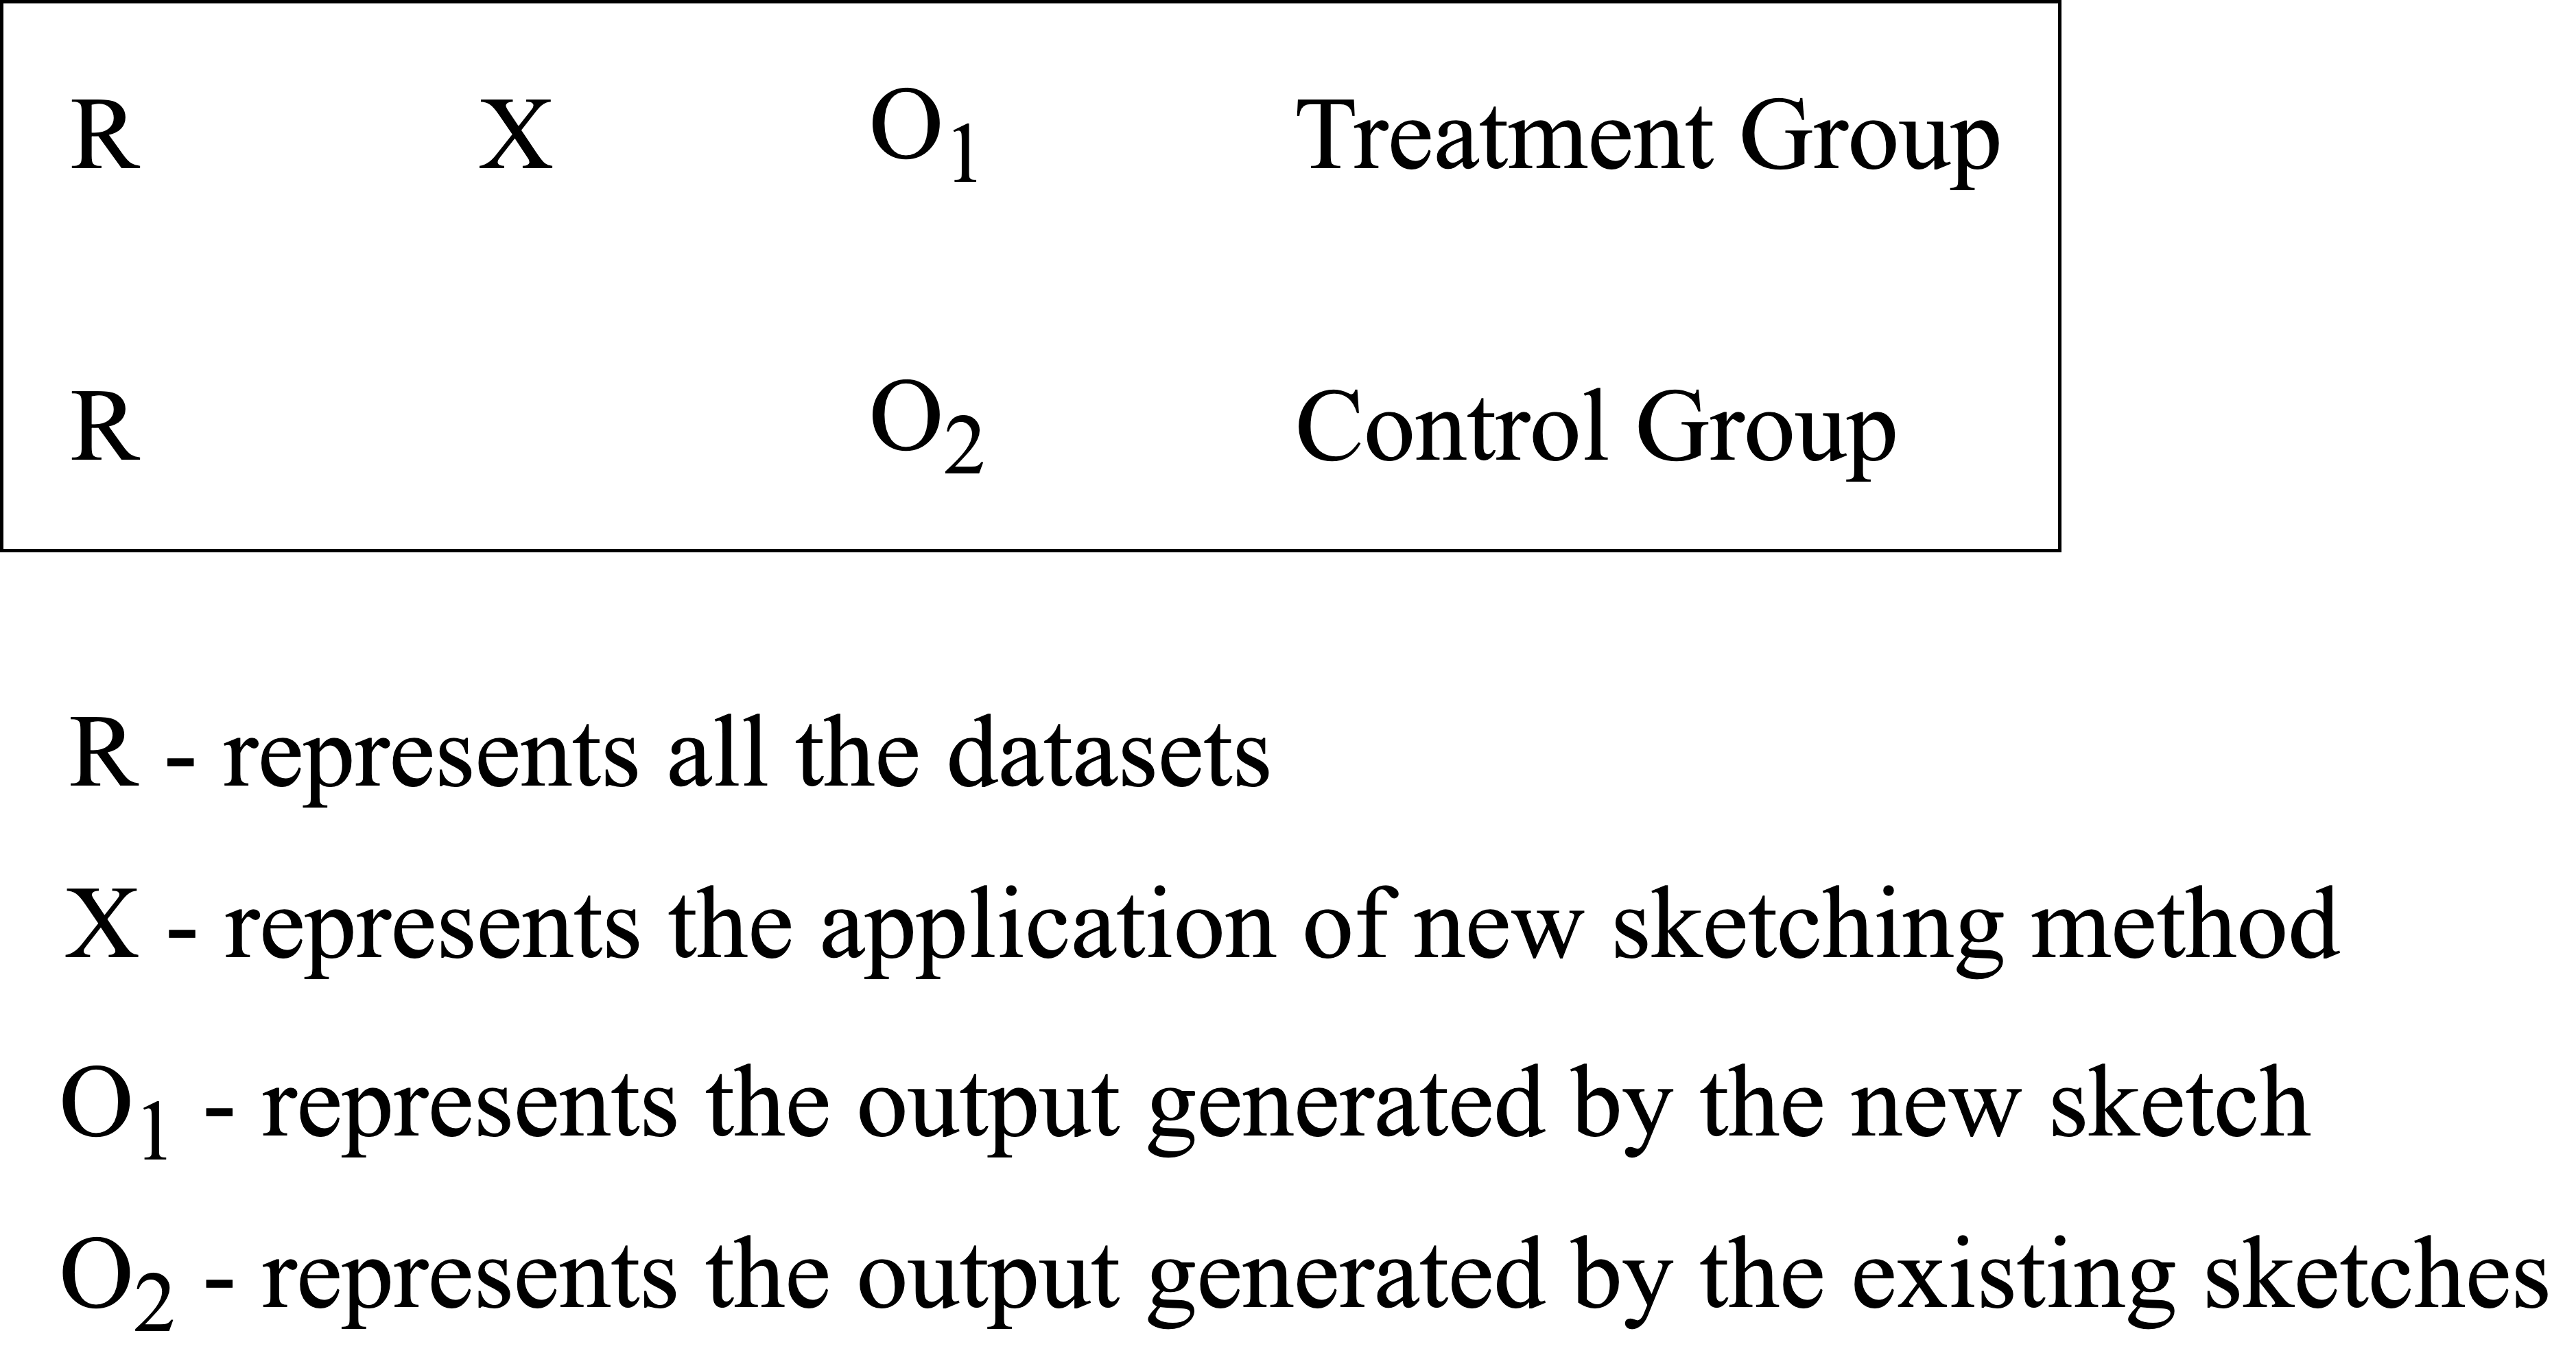
\includegraphics[width=0.7\textwidth]{methodology}
    \caption{Research methodology}
    \label{fig:methodology}
\end{figure}
\section{Outline of the Dissertation}

\paragraph{}
This dissertation spans across the following 6 chapters.

\begin{enumerate}
    \item \textbf{Introduction}\\
          Chapter 1 gives an introduction to the research work carried out through several sections. First, it describes the background of the research. Then it establishes the motive for the research through the sections, research problem and research questions, aims and objectives and the justification for the research. The introduction chapter also includes the research methodology which describes the process of data collection and the delimitations of the scope of the research.

    \item \textbf{Literature review}\\
          Chapter 2 lays out a comprehensive review done on the related work of this research. It includes an introduction to the graphs and their representations, streaming graphs and graph summarization. Here much emphasis has been given for the streaming graph summarization as it is more closely aligned with the topic of the research. In this section, a summary of each streaming graph summarization technique that will be re-implemented and evaluated in chapter 5 and chapter 6 is presented.

    \item \textbf{Research design}\\
          Chapter 3 consist of the research design. In this chapter, the overall architecture of the test suite is explained while focusing on its relevance in answering the research questions in \autoref{section:research_questions}. Furthermore, all the datasets that will be used for the benchmarking purposes will be mentioned along with their origin and the basic properties such as the number of edges in the graph. The ethical implications of using the aforementioned datasets will be discussed as well.

    \item \textbf{Implementation}\\
          Chapter 4 will explain the implementation details of the test suits in a much granular level. It will also address the issues that pertained to the implementation and the workaround the were followed in order to solve them. However, this chapter would not include the full codes for the implemented algorithms; which will appear in the \autoref{appendix:codes} of this dissertation.

    \item \textbf{Results and evaluation}\\
          Chapter 5 contain the results obtained after benchmarking the implemented sketches against the selected datasets.

    \item \textbf{Conclusion}\\
          Chapter 6 discuss how the results mentioned in Chapter 5 has addressed the research questions. An emphasis will be given in highlighting the contribution of this research work to the scientific world. Implications of further research will also be discussed in this chapter.
\end{enumerate}
% \section{Definitions}

\todo
\section{Delimitation of Scope}

\subsection{In scope}

\begin{itemize}
    \item The project will improve upon the existing streaming graph sketching techniques.
    \item The efficiency of running queries on various graph properties after the sketching process will be improved.
    \item New sketching techniques along with the implementations of related work will be evaluated on a parallel framework.
\end{itemize}

\subsection{Out of scope}

\paragraph{}
There exists a number of methods for graph partitioning. The effect of these partitioning techniques will affect the results of the query efficiency and thus they will be considered during the experimentation phase and in presenting results. However, no significant work or separate evaluation will be done with regard to graph partitioning. Improving partitioning techniques will be considered as out of scope for this research.

\paragraph{}
There are many security concerns with regard to the partitioning of streaming graphs and running sketching algorithms in a distributed environment. However, the security aspects of sketch creation and partitioning will be considered as out of scope for this research as they are trivial to the holistic view of the research question, i.e, efficient sketching of streaming graphs.
\chapter{Literature Review}

\section{Graphs in the real world}

\paragraph{}
There are many real-world datasets that can be mapped into graphs. As an example, the users in a social network and the interactions between them\cite{mishra_modelling_2014}, details about the packet transfer in a computer network\cite{ahmat_graph_nodate} and a large citation database with authors of the research papers and their publications\cite{cui_citation_nodate} are some of the real-world scenarios that could be mapped into graphs perfectly. This makes the discovery of the properties of the original dataset more feasible using graphs algorithms. Apart from the computation needs, datasets are often represented as graphs for visualization purposes as well\cite{wang_survey_2015}.

\paragraph{}
With the increase of the number of devices connected to the internet and the reduction of the cost of the storage media, the amount of collected data has grown by an exponential rate. Due to the sheer volume of the original datasets, the graphs produced from these datasets are also massive in size. Real-world graphs have various other properties such as empirically, most real-world graphs sparse and obey skewed power-law degree distribution\cite{xie_distributed_2014}.

\paragraph{}
The properties of a graph that needs to be retrieved vary widely with the application scenario. As an example, in a social network, it would be vital in finding the heavy hitter edges depicting the interaction between users or reachability of nodes showing how close the specific users are related. Model of a computer network would benefit with queries in finding heavy hitter nodes indicating possible destinations and sources of attacks originating within the network.

\paragraph{}
Keeping these massive graphs in memory has become unrealistic with the large capacity that is required to store them. There are many challenges that lie in utilizing massive graphs to derive knowledge through their properties while keeping them stored in secondary storage devices. This becomes easily evident in a scenario of a social network like Facebook\cite{ching_one_2015} or Twitter\cite{kwak_what_2010} where millions of user accounts interact with each other adding a large number of edges to the graph in a unit time.

\paragraph{}
Most importantly, many of the real-world scenarios get mapped into graph streams rather than static graphs. Modern datasets do not stay small nor do they stay static. Retrieving the properties of this constantly evolving graph in realtime poses many difficulties\cite{kumarage_efficient_2017}.
\section{Streaming graphs}

\paragraph{}
Graphs can be divided into two as static graphs and streaming (dynamic) graphs. Static graphs are those which do not change over time while streaming graphs are the ones which do get updated over time. These update operations could be insertion or deletion of nodes and edges.

\paragraph{}
Determining the properties of streaming graphs is relatively strenuous than static graphs as they are constantly evolving. Usual graph algorithms cannot be run on streaming graphs due to their dynamic nature. Either the updating queries has to be stopped or a separate snapshot of the past should be used while running the static graph algorithms on a streaming model. If there is a need for processing the graph while streaming, separate streaming graph algorithms have to be devised\cite{mcgregor_graph_2014}. This is made even more difficult with the speed with which the graph is being updated. High throughput of update queries requires any other types of queries to be run efficiently and as fast as possible in an unblocking manner.

\paragraph{}
Real-world streaming graphs could grow very large in size. Therefore these graphs are often stored as partitions in different machines over a network rather than in a single location.
\section{Graph partitioning}

\paragraph{}
The size of modern datasets has become too large to be fit into a single machine. It has become unrealistic to try to process the graphs mapped to these massive datasets while keeping them in the memory of a single node. Hence there exists a need to partition those large scale graphs into multiple machines. The communication between groups should be minimal to run graph algorithms on the whole graph effectively.

\paragraph{}
However, graph partitioning is an NP-hard problem\cite{noauthor_simplified_nodate}. Therefore the graph partitioning algorithms are only able to give sub-optimal solutions as of this date and thus a good streaming graph partitioning algorithm is impossible\cite{stanton_streaming_2012}.

\subsection{Online and offline graph partitioning}

\paragraph{}
Graph partitioning algorithms can be mainly divided into two, such that, Online Graph Partitioning Algorithms and Offline Graph Partitioning Algorithms. The offline partitioning algorithms such as METIS\cite{karypis_fast_1998}, Chaco\cite{hendrickson_chaco_1993}, SBV-cut\cite{kim_sbv-cut:_2012} need to load the entire graph into the memory for the algorithm to be run. But the online partitioning algorithms like PreferBig\cite{stanton_streaming_2012} and HoVerCut\cite{sajjad_boosting_2016} keeps a buffer of the edge streams and process them when the buffer gets full.

\subsection{Edge-cut and Vertex-cut methods}

\paragraph{}
Graph partitioning can also be divided according to the cutting method; which is Edge-cut and Vertex-cut\cite{xie_s-powergraph_nodate}. Edge-cut tries to evenly assign the vertices to each partition by cutting the vertices while the vertex-cut ties to evenly assign the edges to each partition by cutting the vertices. The edge-cut method could leave some partitions with a higher number of edges than others. Therefore the vertex-cut techniques generally achieve better performance than edge-cut techniques\cite{gonzalez_powergraph_nodate} for graphs which obeys the power-law degree distribution.

\paragraph{}
It is difficult to evaluate the properties of a graph with high volume and throughput even after the partitioning process as the whole graph would have to be processed despite the partitioning. Graph summarization is a technique used in dealing with these massive graphs.
\section{Graph summarization}

Reducing the complexity of a graph while retaining some of its original properties is known as graph summarization. These summaries often incur an error when running algorithms due to the loss of information. As depicted in \autoref{fig:summarization}, the result of the same algorithm executed on the graph summary will be approximately equal to that of the result of the original graph depending on the compression ratio and a variety of other factors. But usually, when it comes to real-world massive graphs such as social networks, it is enough to obtain approximations instead of the exact answers with a reduced computational cost.

\begin{figure}[H]
    \centering 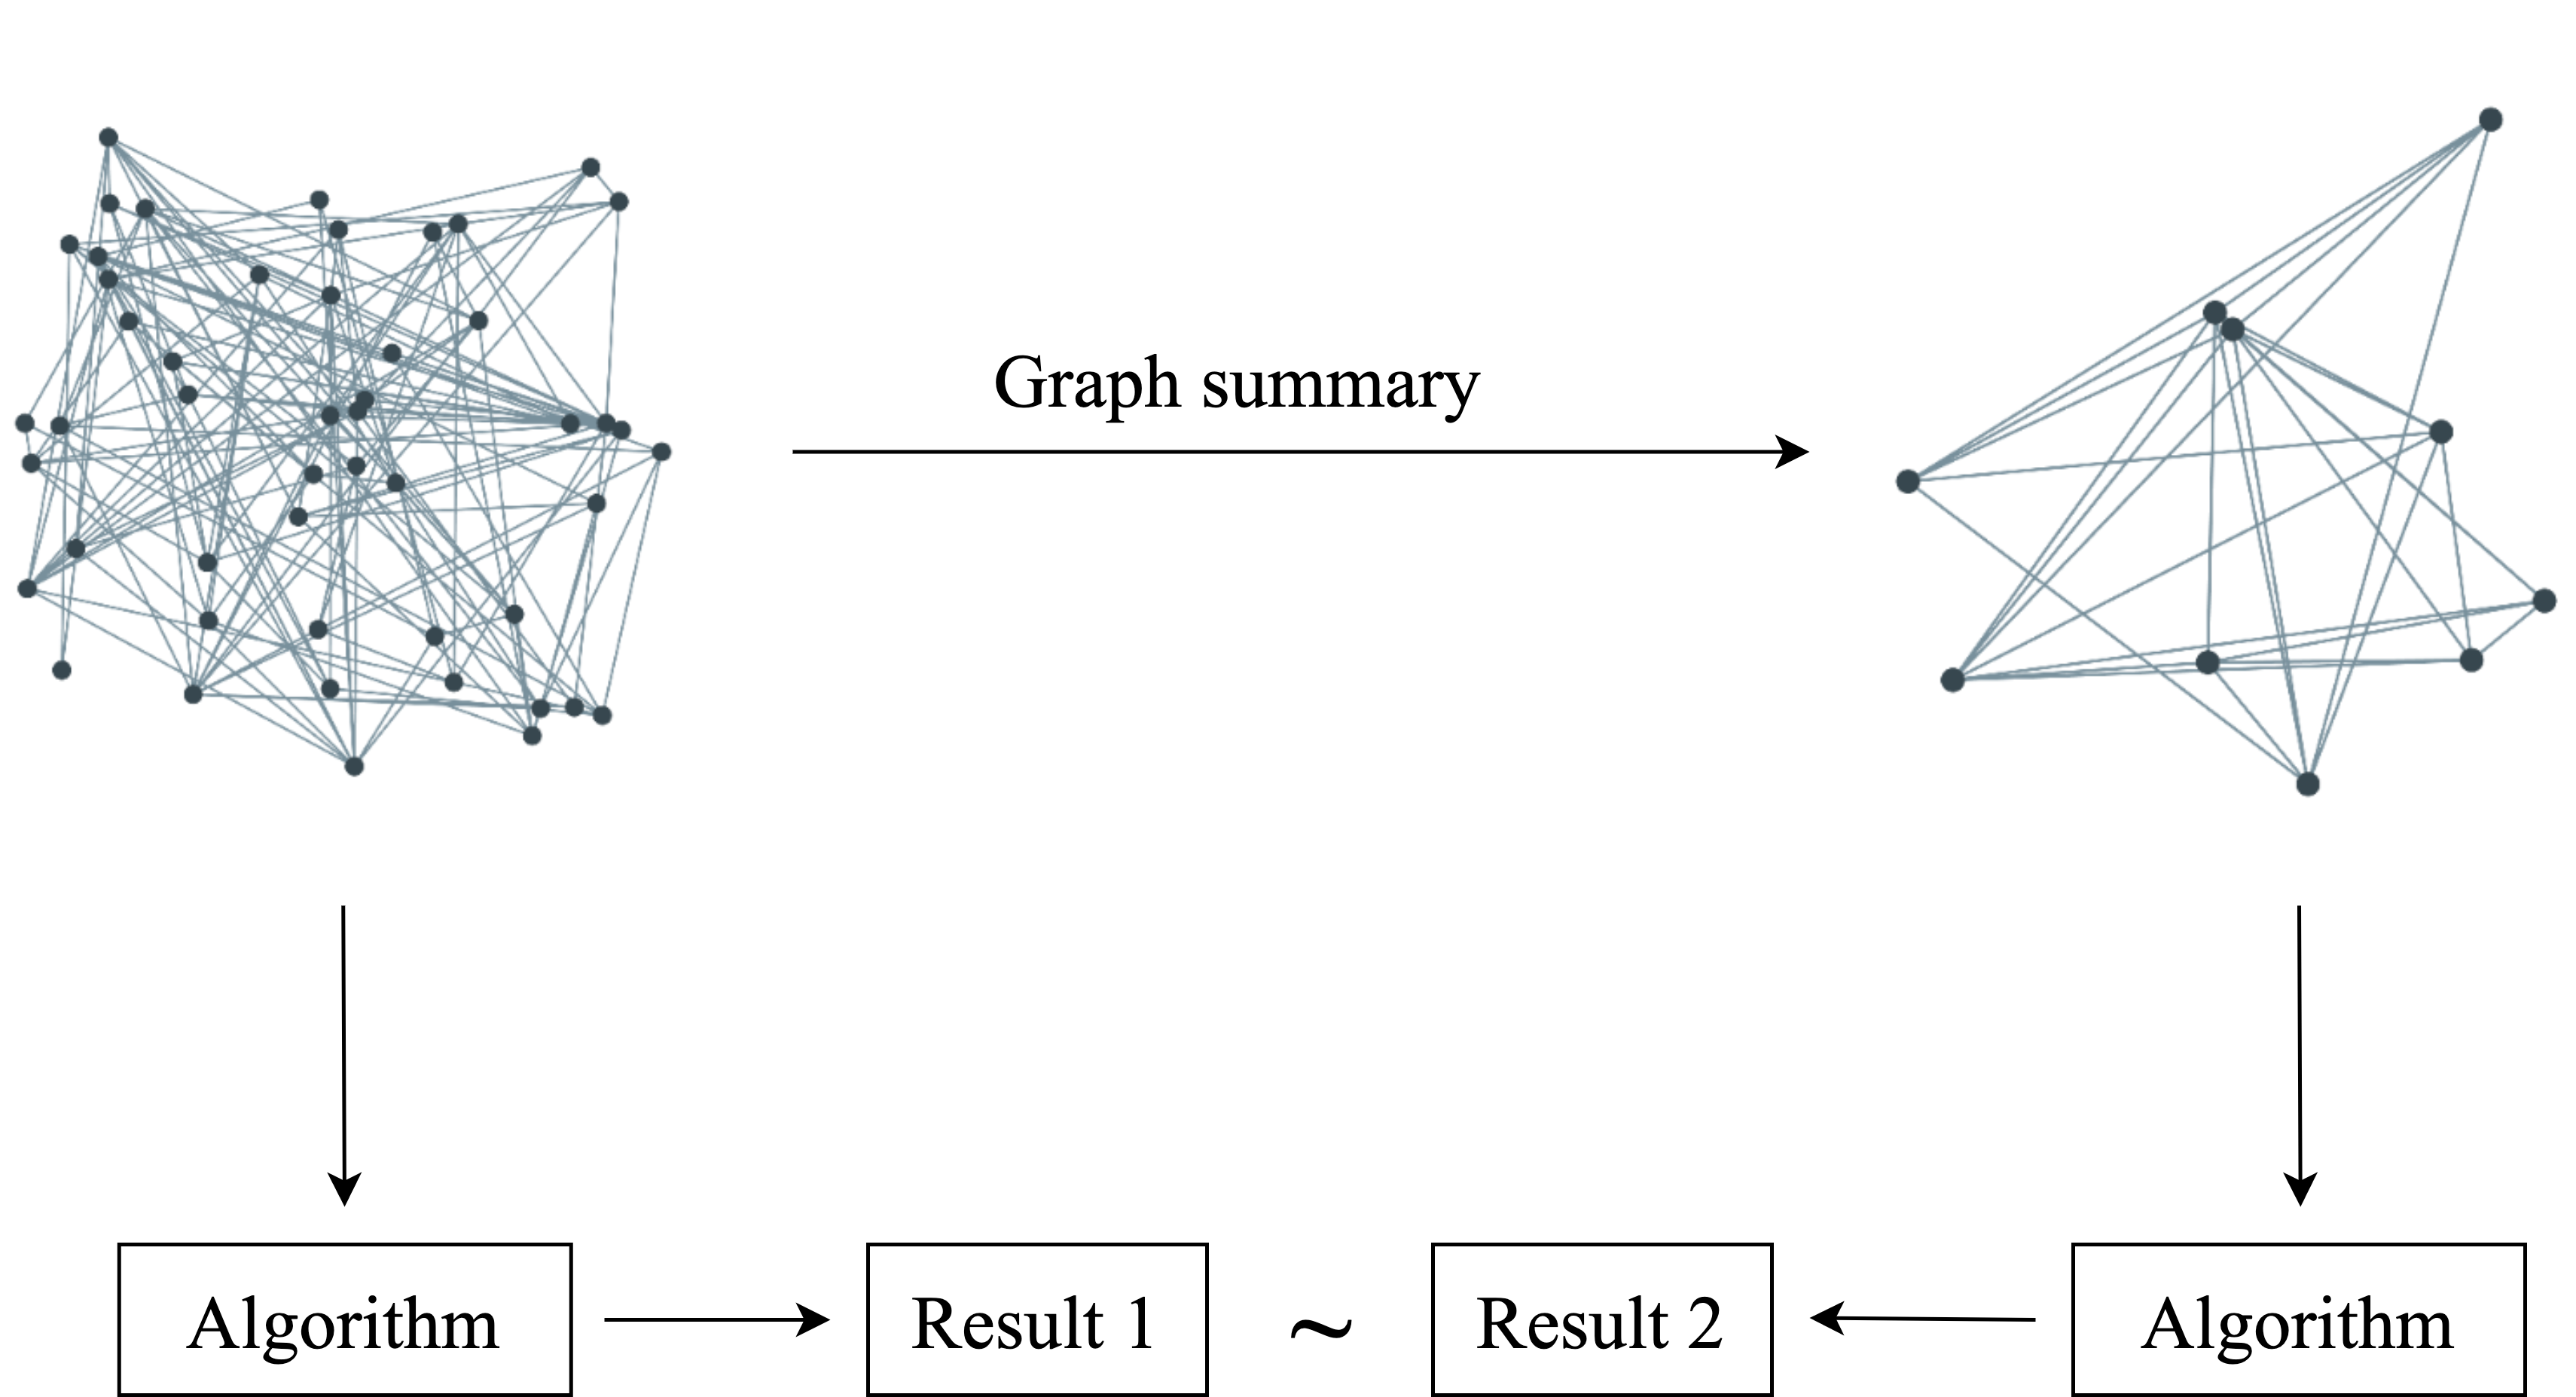
\includegraphics[width=0.7\textwidth]{summarization}
    \caption{Graph summarization}
    \label{fig:summarization}
\end{figure}

\subsection{Benefits of graph summarization}

\paragraph{}
Graph summarization has a wide range of benefits\cite{liu_graph_2018}.

\begin{itemize}
    \item \textbf{Speedup of graph algorithms and queries}\\
          It incurs a huge computational cost to run the regular graph algorithms on massive graphs. Graph summarization always produces a smaller version of the graph, making it easier to run different queries and algorithms on the summarized sketch. The result produced by the summarized sketch will have an accuracy tradeoff when compared with the result that will be given by the original graph\cite{riondato_graph_nodate}. However, the tradeoff is acceptable in some scenarios where the speedup gain is very large.

    \item \textbf{Reduction of data volume and storage}\\
          It takes significant storage to store a large graph on storage media. The space needed for storing the entire graph will be at least \(O(E+V)\). This is not achievable in some scenarios. As an example, an IoT device with limited storage, monitoring a data stream will not be able to store the entire stream in its memory. Graph summarization can be used to reduce the complexity of the original graph in order to reduce the space needed to store the graph\cite{seo_effective_2018}.

    \item \textbf{Visualization\cite{dunne_motif_2013, jin_eco_nodate}}\\
          There are two main issues pertaining to user analysis of large scale streaming graphs. It will be difficult to fit the entire graph in memory so that the visualization algorithm could run on it. Even if the former was achievable, it would be cumbersome to analyse the original graph because of the high number of vertices and edges. Graph summarization could avoid this “hairball” visualization problem\cite{schulz_grooming_2013}.

    \item \textbf{Noise elimination}\\
          Real word graphs are riddled with hidden and erroneous links and labels. Removing the noisy information makes it easier to analyse the graph. Graph summarization could essentially act as a process in filtering out the noise and reveal more interesting features\cite{zhang_discovery-driven_2010}.

    \item \textbf{Privacy preservation}\\
          This can be a crucial step in preserving privacy when releasing the aggregate numbers. Graphs are summarized with the purpose of preserving the privacy of the original dataset\cite{shoaran_zero-knowledge_2013}.
\end{itemize}

\subsection{Applications of graph summarization}

\paragraph{}
Restating the aforementioned, graph summarization has a wide range of benefits and thus used in different industrial and research applications. Apart from these scenarios, there are some other applications of graph summarization such as clustering\cite{cilibrasi_clustering_2005}, classification\cite{hutchison_compression_2006}, community detection\cite{chakrabarti_fully_nodate}, outlier detection\cite{smets_odd_2011, akoglu_opavion_2012}, pattern set mining\cite{mampaey_tell_2011} and finding sources of infection in large graphs\cite{prakash_spotting_2012}.

\paragraph{}
During this research, our aim lies in query optimization through graph summarization.

\subsection{Challenges of graph summarization}

\paragraph{}
There are many challenges involving in graph summarization\cite{liu_graph_2018}.

\begin{itemize}
    \item \textbf{Data volume}\\
          Graph summarization primarily intends to deal with the large volume of data. Therefore handling the original dataset in order to create the summary sketch itself is a cumbersome task.

    \item \textbf{Complexity of data}\\
          Some graphs can be heterogeneous in nature, making it increasingly more difficult to summarize the graph. Considering the heterogeneity of the nodes during the summarization may lead to a complex architecture\cite{kivela_multilayer_2014}.

    \item \textbf{Definition of interestingness}\\
          Definition of interestingness depends on the application scenario and user preference. It is difficult to determine the acceptable tradeoffs for a specific summarization without the domain knowledge.

    \item \textbf{Evaluation}\\
          There are a number of parameters that can be used for the evaluation of graph summaries. A summary is considered good if it efficiently supports both the local and global queries with high accuracy. But in a scenario where visualization is involved, qualitative criteria would have to be used for evaluation as it is subjective to the opinion of the domain experts.

    \item \textbf{Change over time}\\
          Usually, real-world graphs are streaming, thus the summaries should also evolve with time\cite{leskovec_graphs_2005}.
\end{itemize}

\subsection{Types of graph summarization}
\label{section:sumtypes}

\paragraph{}
Graph summarization methods can be categorized according to various criteria.

\paragraph{}
One classification is, according to the nature of the input data; static graph summarization and streaming graph summarization. Static graphs do not evolve with time, thus making it impossible to use the same methods to summarize both static and streaming graphs. Due to their dynamic nature, an extra effort has to be spent on summarizing the streaming graphs. In this research, we will only focus on summarizing streaming graphs.

\paragraph{}
Summaries can also be classified considering the nature of the input graph; homogeneous and heterogeneous. We will only consider about homogenous summaries during this research.

\paragraph{}
There are a few core techniques used when summarizing graphs\cite{liu_graph_2018}.

\begin{itemize}
    \item \textbf{Grouping or aggregation based}\\
          Nodes are aggregated into ‘supernodes’ in order to reduce the complexity of the original graph. Edge-grouping methods aggregate multiple edges into single edges.

    \item \textbf{Bit compression based}\\
          Bit compression minimizes the number of bits needed to store the input graph. There are lossy compression methods as well as lossless compression methods.

    \item \textbf{Simplification or sparsification based}\\
          This approach removes the less important nodes and edges producing a sparsified graph.

    \item \textbf{Influence based}\\
          Influence based summarization aims to provide insights into the influence propagation of a graph. This type of summarization can be specially useful in scenarios where social networks are considered.
\end{itemize}

\subsection{Streaming graph summarization}

\paragraph{}
Summarizing graph streams is more difficult than summarizing a static graph due to the constant flow of data. Underlying original graph is constantly updated while it is being summarized. Therefore the summarization process has to be done in realtime. Almost any static graph summarization technique could be used with streaming graph snapshots within specific time frames. However, mining information using aggregate time snapshots of data could very well be an unrealistic goal in a massive streaming graph. Thus sophisticated sparsification techniques have to be derived in order to summarize streaming graphs.

\subsubsection{CountMin\cite{cormode_improved_2003}}

\paragraph{}
CountMin could be considered as the pioneering work in summarizing data streams which are directly related to our research. CountMin is a data structure that is used for frequency approximation queries. The underlying idea behind the CountMin data structure is to hash the aggregated frequencies of the edges using multiple hash functions into predefined blocks as indicated in \autoref{fig:countmin}. A fixed-size will be stated at the time of the creation of the CountMin sketch and irrespective of the volume of data stored, the size of the sketch does not have to be changed. The major drawback in following this procedure is that the error of the queries reduce as more and more data is introduced to the sketch. However, despite these weaknesses, CountMin can be considered as a good generalized sketch at the time as many other sketches described in the literature are good for one single pre-specified aggregate computation. Therefore CountMin approach is not restricted to streaming graphs but other applications as well\cite{cormode_improved_2003}.

\begin{figure}[H]
    \centering 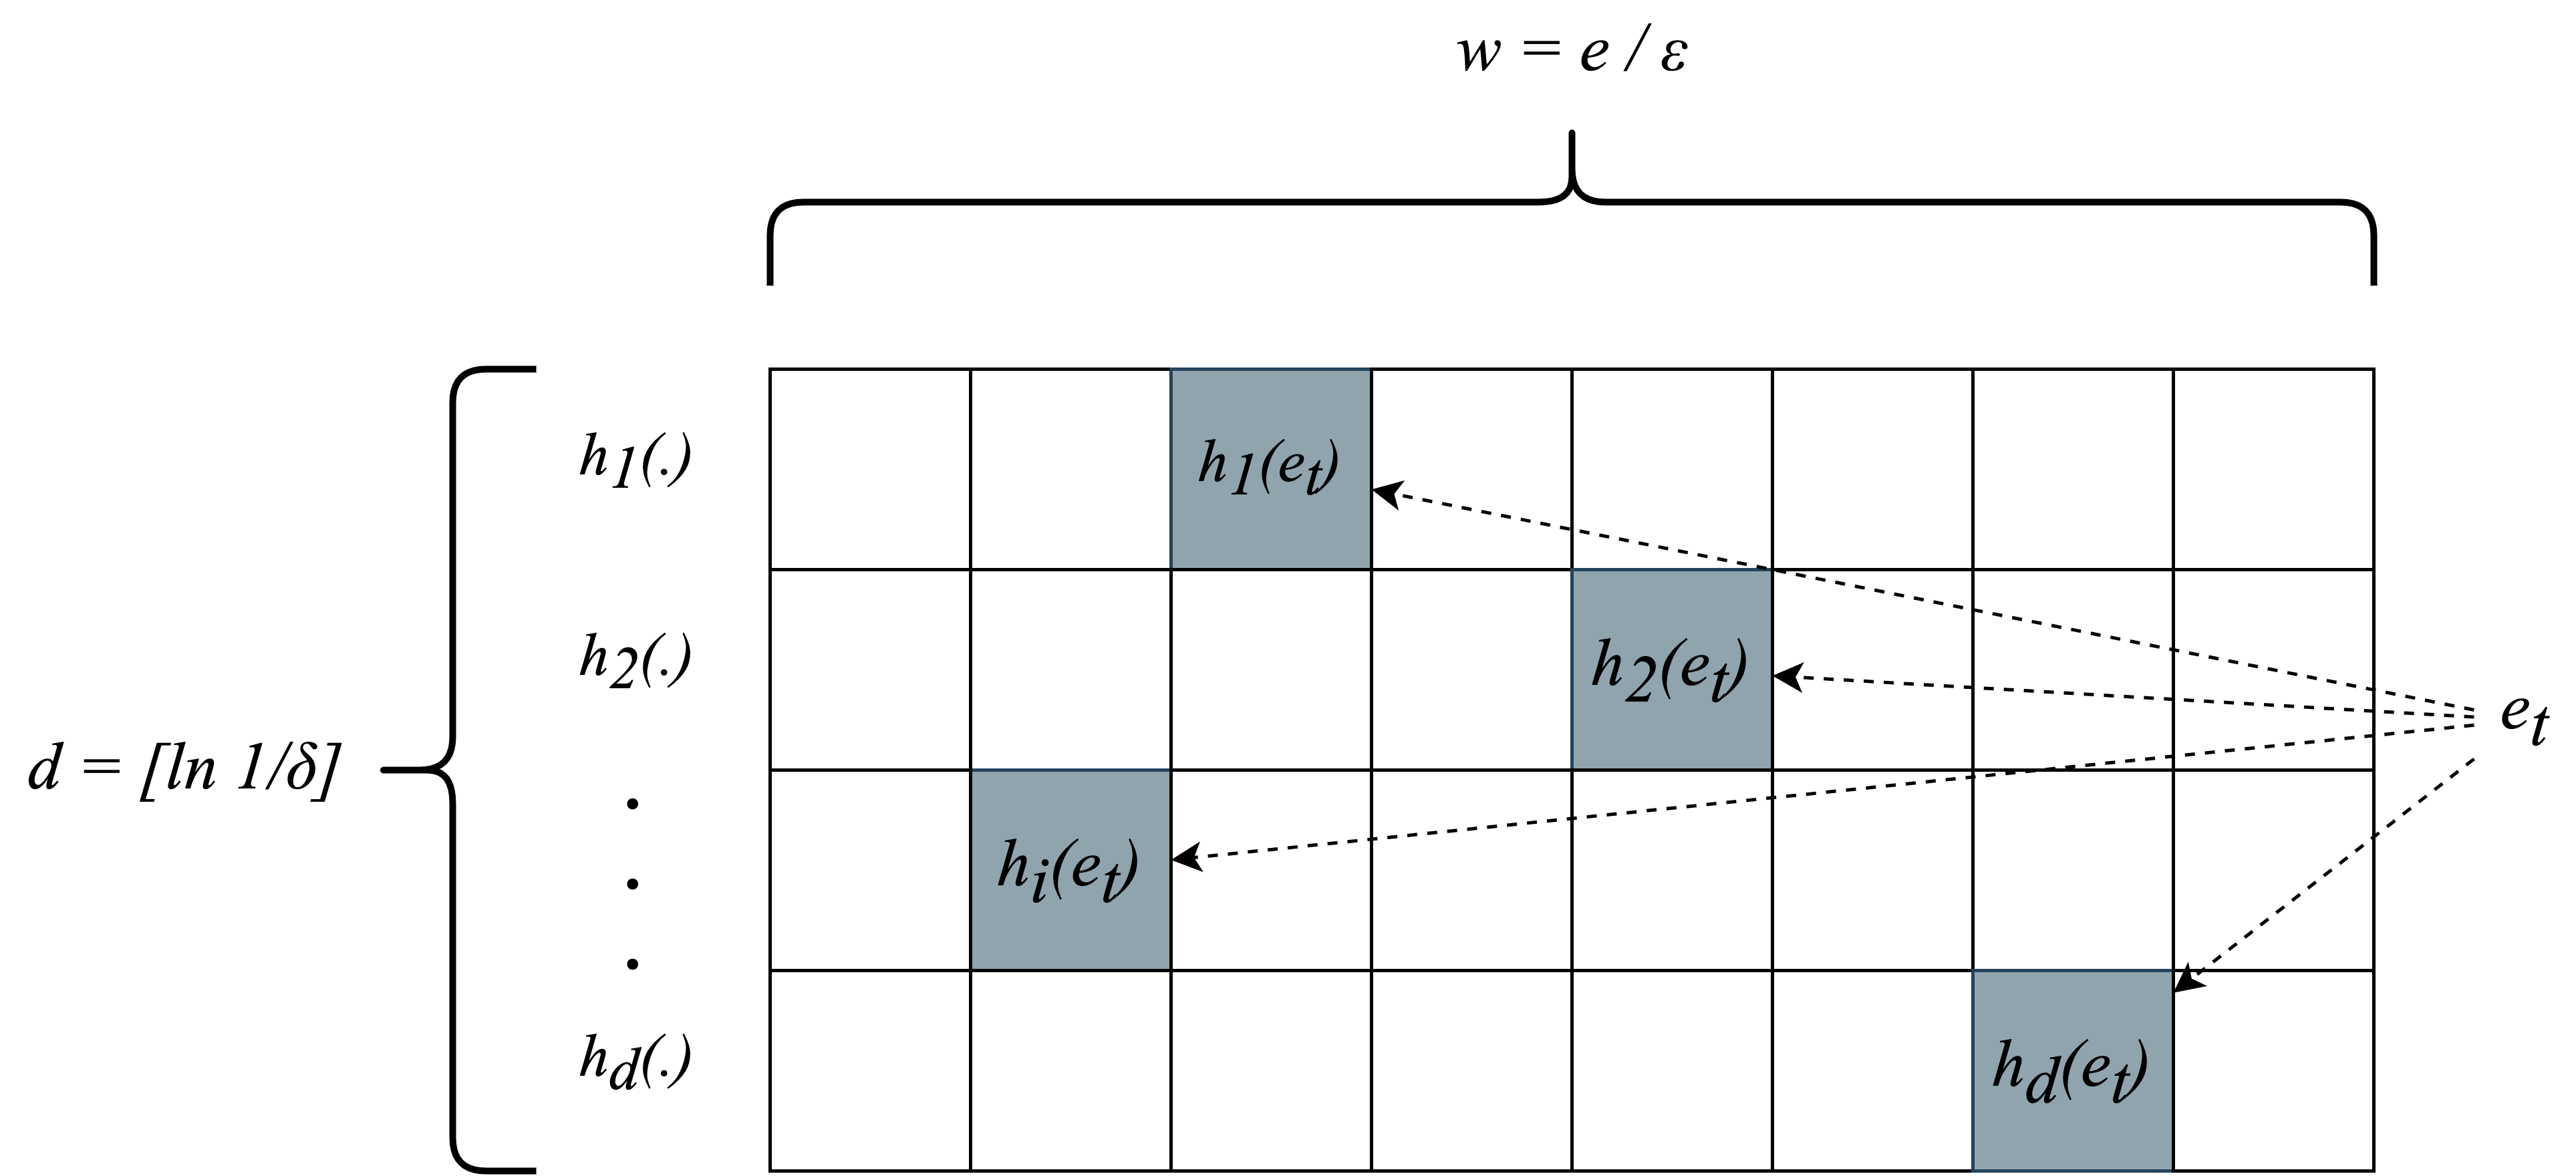
\includegraphics[width=\textwidth]{countmin}
    \caption{CountMin sketch}
    \label{fig:countmin}
\end{figure}

\subsubsection{gSketch\cite{zhao_gsketch:_2011}}

\paragraph{}
gSketch is an extension of CountMin data structure. But unlike CountMin sketch, this is specifically geared towards summarizing graph streams. gSketch is based on one of the two assumptions that,

\begin{itemize}
    \item A graph stream sample is available.
    \item Both graph stream sample and a query workload sample are available.
\end{itemize}

\paragraph{}
As per the previous sketching technique, CountMin, a global sketch is created for the entire graph stream. The disadvantage of this method is that any structural properties present in the graph stream are completely ignored throughout this process. gSketch tries to avoid by considering the underlying structural properties of the graph.

\paragraph{}
The speciality of gSketch is to pre-process the stream samples and creating sketch partitions as indicated in \autoref{fig:gsketch}. Its goal is to maintain sufficient frequency uniformity within each localized sketch so that the query estimation can be optimized over the entire graph stream.

\begin{figure}[H]
    \centering 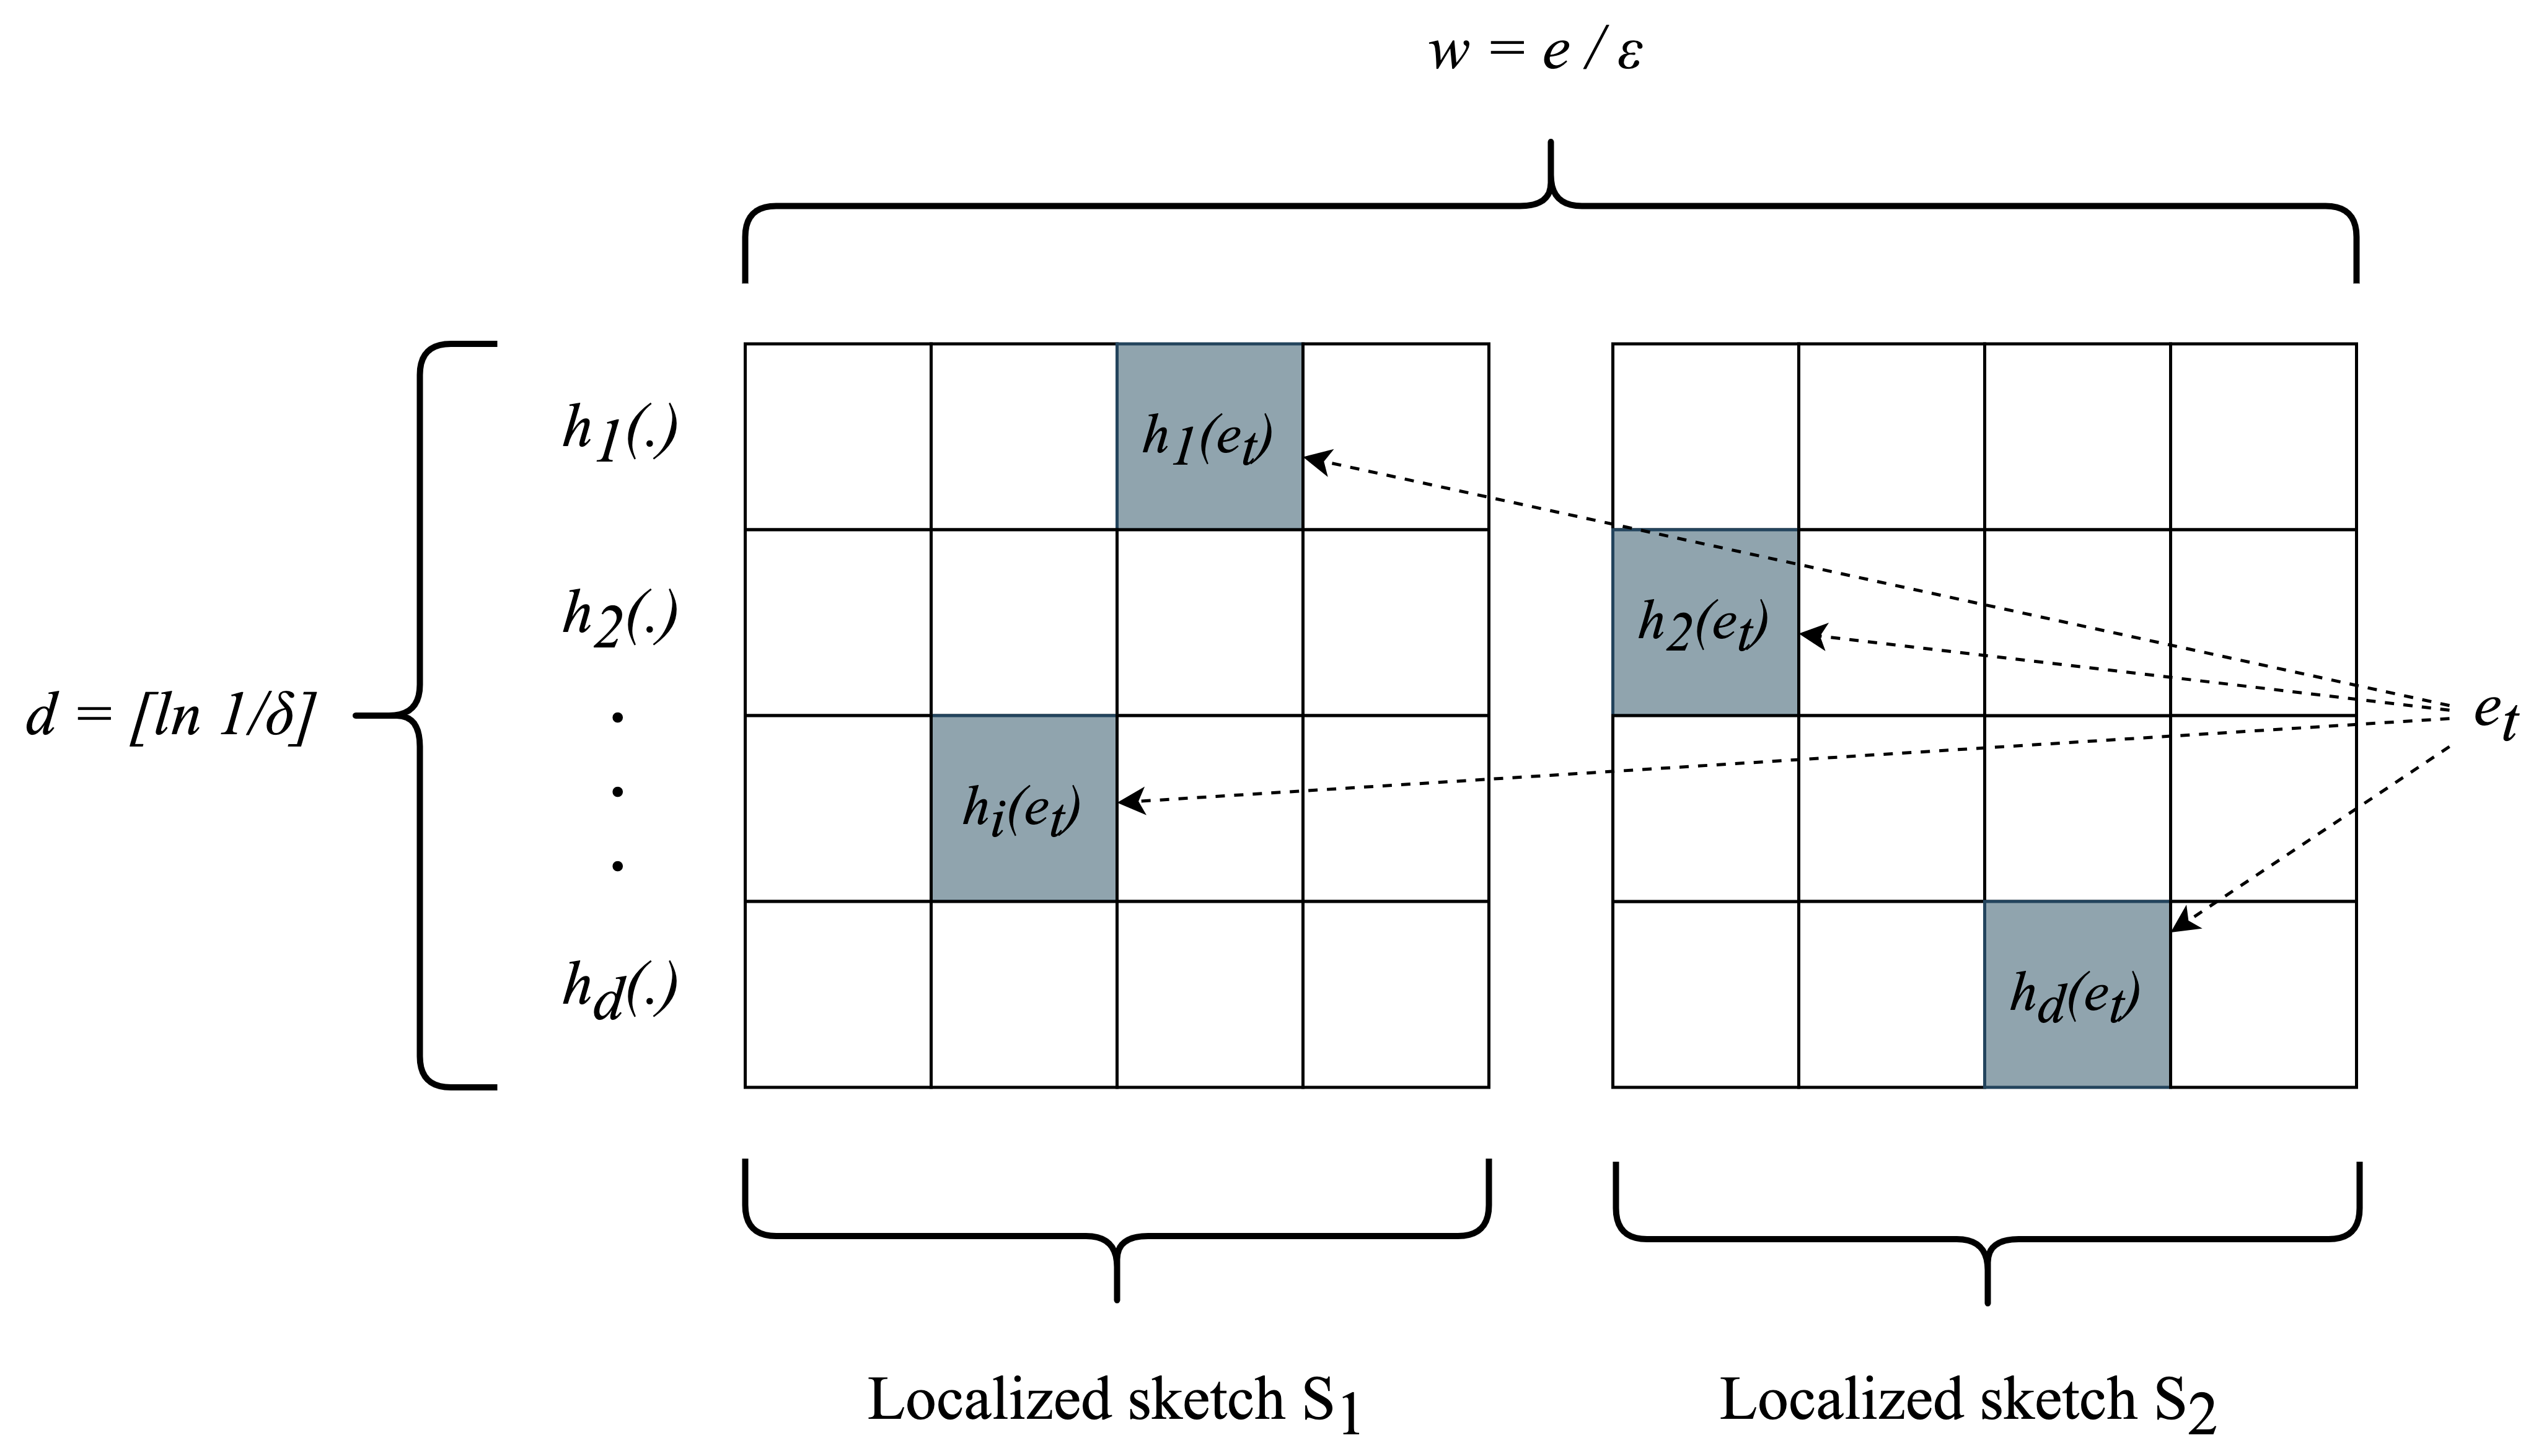
\includegraphics[width=\textwidth]{gsketch}
    \caption{gSketch sketch}
    \label{fig:gsketch}
\end{figure}

\subsubsection{TCM\cite{tang_graph_2016}}

\paragraph{}
Approximate Frequency Count sketches store aggregated frequencies of edges in summarized form. When there is a graph stream as indicated in \autoref{fig:afc_sample_stream}, its summarized node sketch and edge sketch would be the mappings described by \autoref{fig:afc_node_sketch} and \autoref{fig:afc_edge_sketch} respectively.

\begin{figure}[H]
    \centering 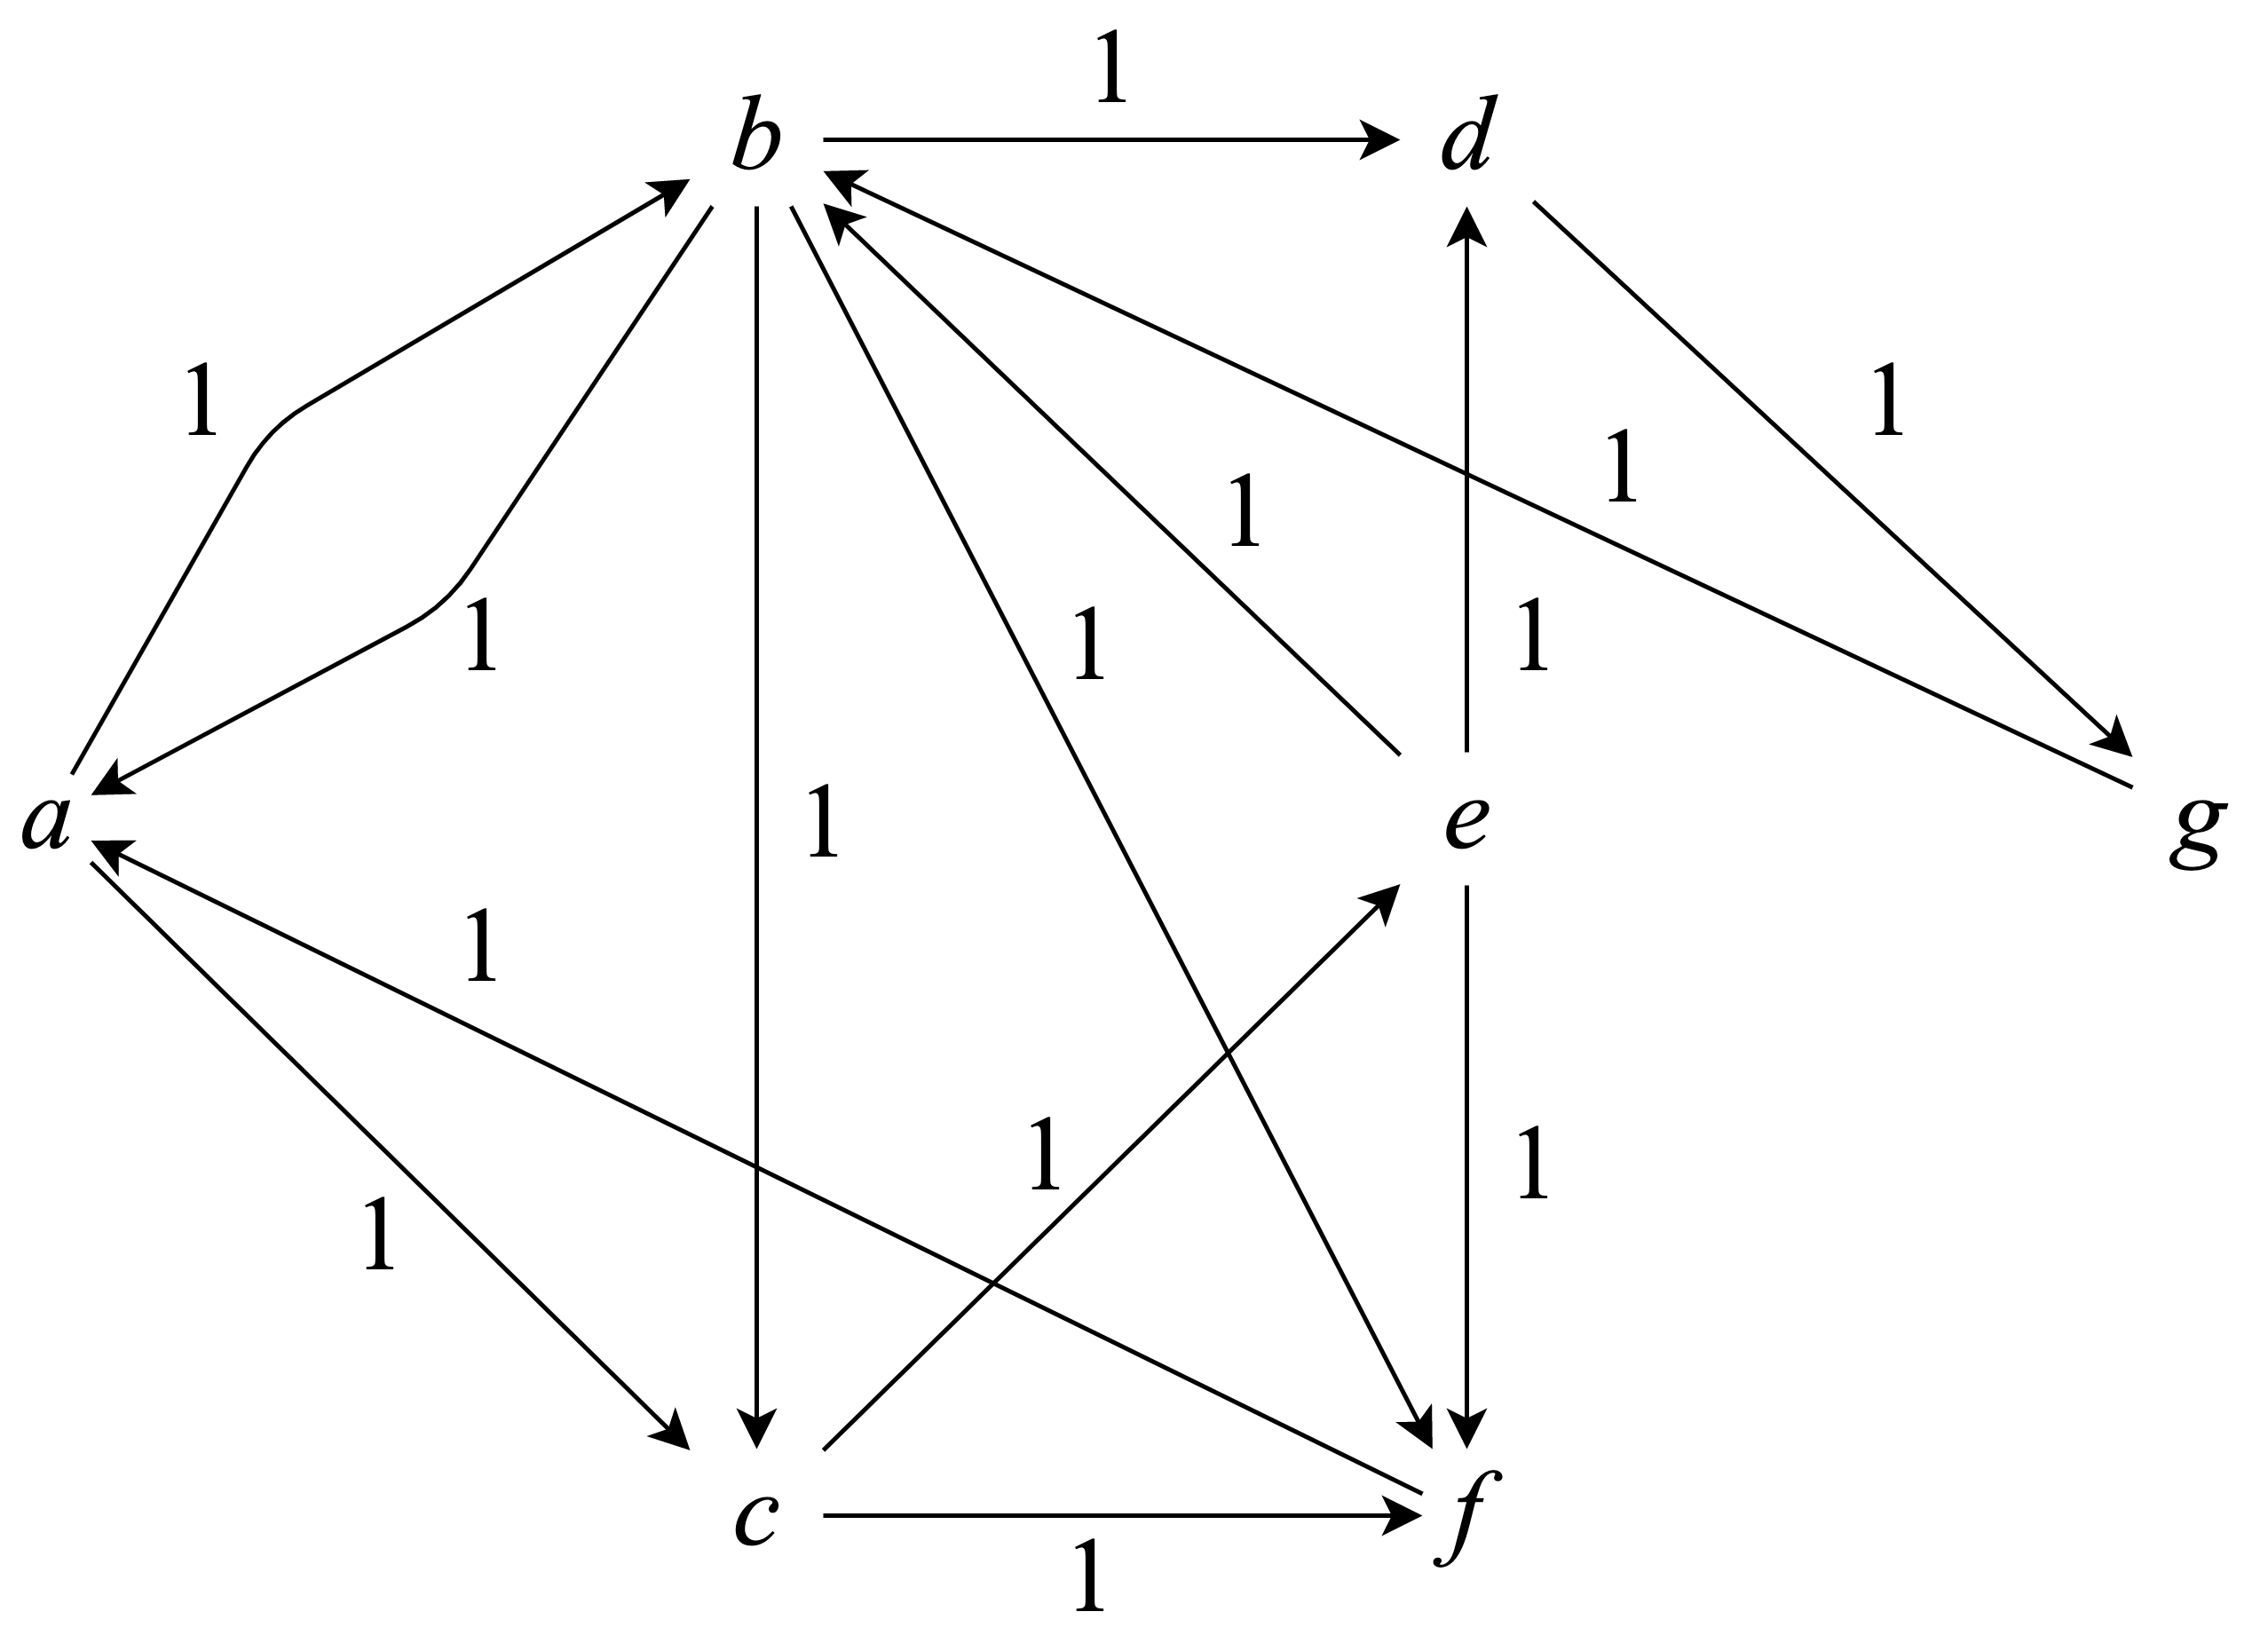
\includegraphics[width=0.5\textwidth]{afc_sample_stream}
    \caption{A sample graph stream}
    \label{fig:afc_sample_stream}
\end{figure}

\begin{figure}[H]
    \centering 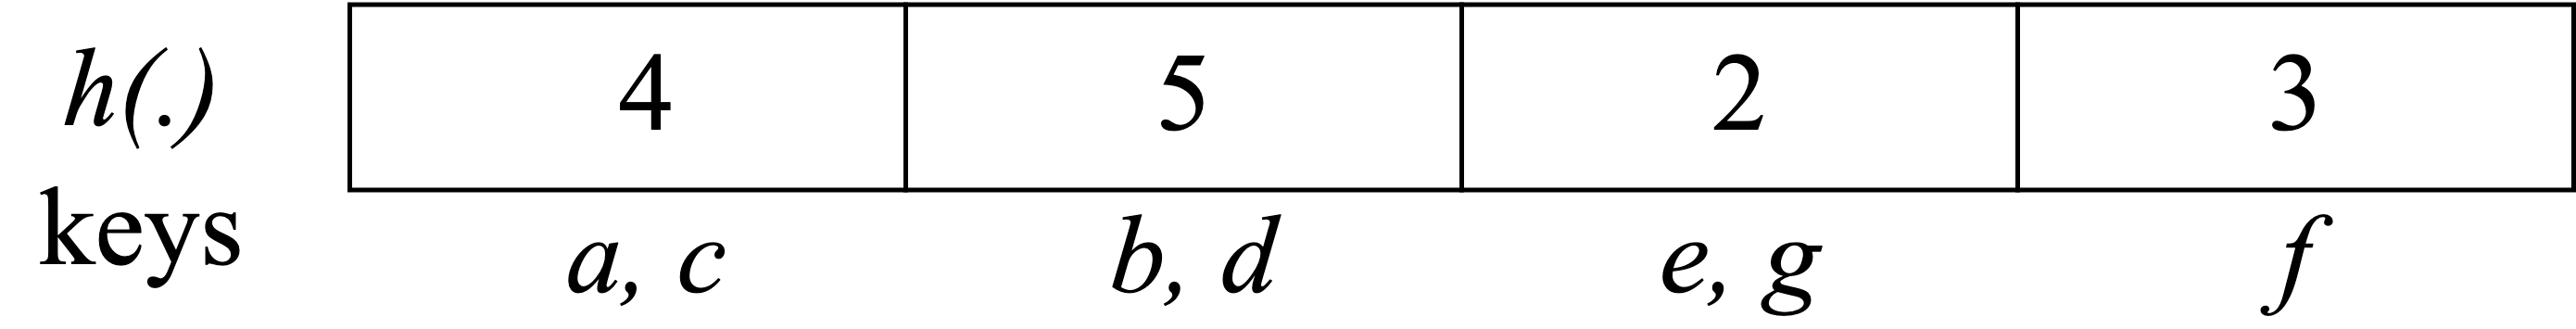
\includegraphics[width=0.5\textwidth]{afc_node_sketch}
    \caption{Node sketch}
    \label{fig:afc_node_sketch}
\end{figure}

\begin{figure}[H]
    \centering 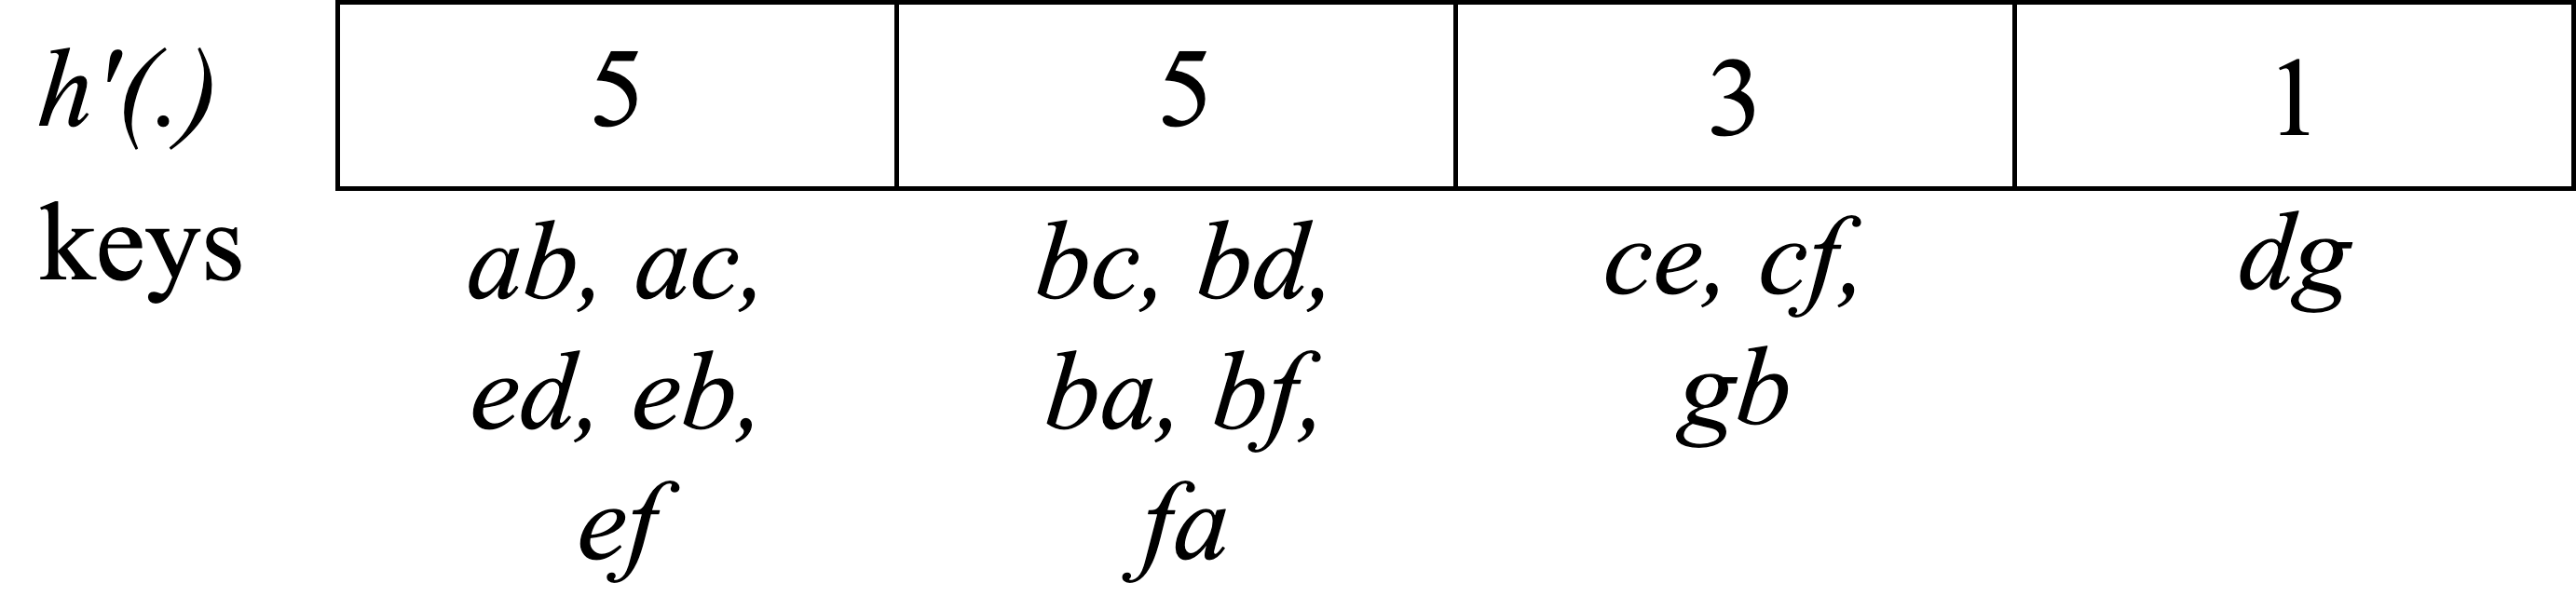
\includegraphics[width=0.5\textwidth]{afc_edge_sketch}
    \caption{Edge sketch}
    \label{fig:afc_edge_sketch}
\end{figure}

\paragraph{}
A disadvantage posed by all the approximate frequency count sketches like CountMin or gSketch is that they do not store the locality of the nodes. Therefore they cannot be used for conditional node queries or queries involving node connectivity. If these queries were to be run, at least some of the information about the locality of nodes has to be retained in the graph synopses. TCM can summarize both node and edge information in constant time. Because of that, it can answer a wide range of queries, unlike its predecessors. The structure of a TCM sketch is depicted in \autoref{fig:tcm}.

\begin{figure}[H]
    \centering 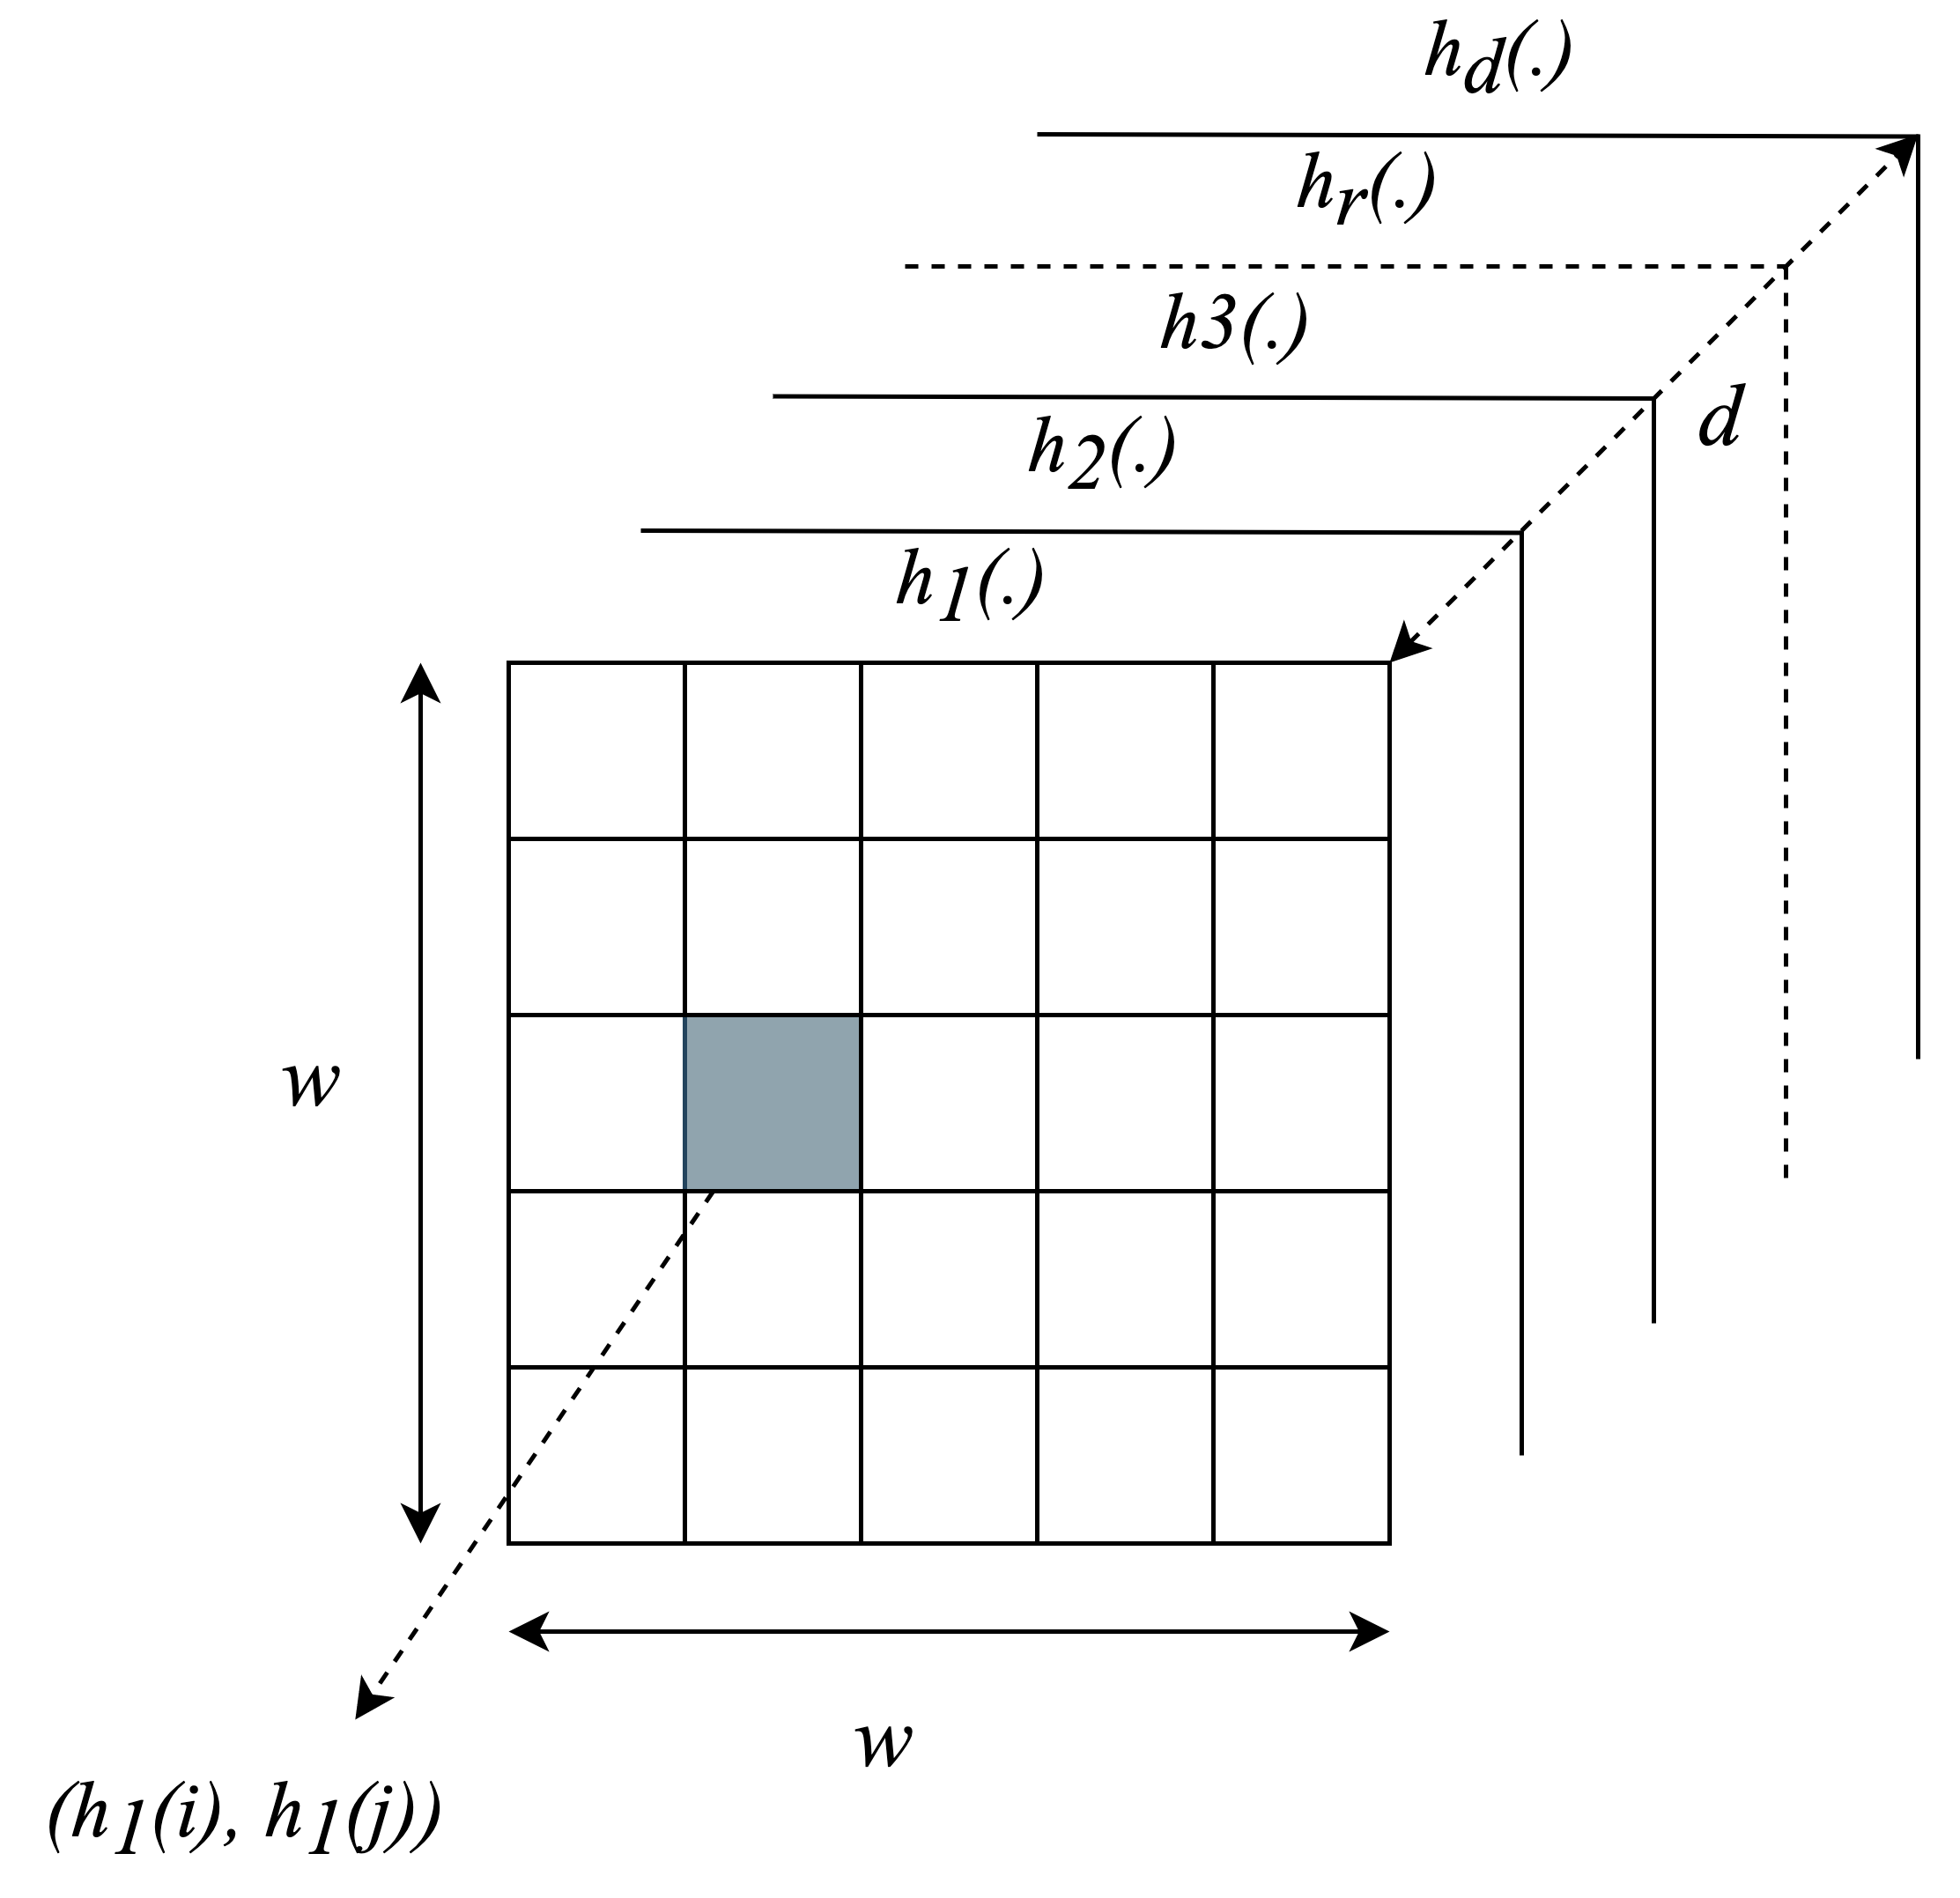
\includegraphics[width=0.7\textwidth]{tcm}
    \caption{TCM sketch}
    \label{fig:tcm}
\end{figure}

\subsubsection{GMatrix\cite{khan_query-friendly_2016}}

\paragraph{}
gMatrix is very similar to TCM and it was proposed in the same year as the TCM. However, gMatrix paper consider about,

\begin{itemize}
    \item reverse hashing queries through pairwise independent hash functions;
    \item alternative options to extend sketch and space-saving synopses for achieving similar functionalities as gMatrix;
\end{itemize}

which the TCM paper does not address.

\subsubsection{GSS\cite{gou_fast_2018}}

\paragraph{}
GSS is the latest graph summarization technique that has been introduced up to date which was published in 2018. Even when using 1/256 memory size of the state of the art graph summarization algorithm, GSS still significantly outperformed it for most queries. The GSS paper points out that even if TCM and gMatrix support all queries in the streaming graphs in contrast to CM sketches\cite{cormode_improved_2003} and gSketch which only supports queries for edges and do not get involved with the topology of the underlying graph, they suffer from poor accuracy. GSS improves upon TCM and gMatrix to increase the accuracy with less memory usage.

\paragraph{}
GSS defines three graph primitives as,

\begin{itemize}
    \item Edge query
    \item 1-hop Successor query
    \item 1-hop Precursor query
\end{itemize}

\paragraph{}
By supporting all these 3 types of queries it is possible to reconstruct the entire graph. Therefore it is also possible to run any kind of query against a sketch which supports all 3 of the above primitives.

\paragraph{}
The intuition behind the basic version of the GSS can be illustrated as below.

\begin{figure}[H]
    \centering 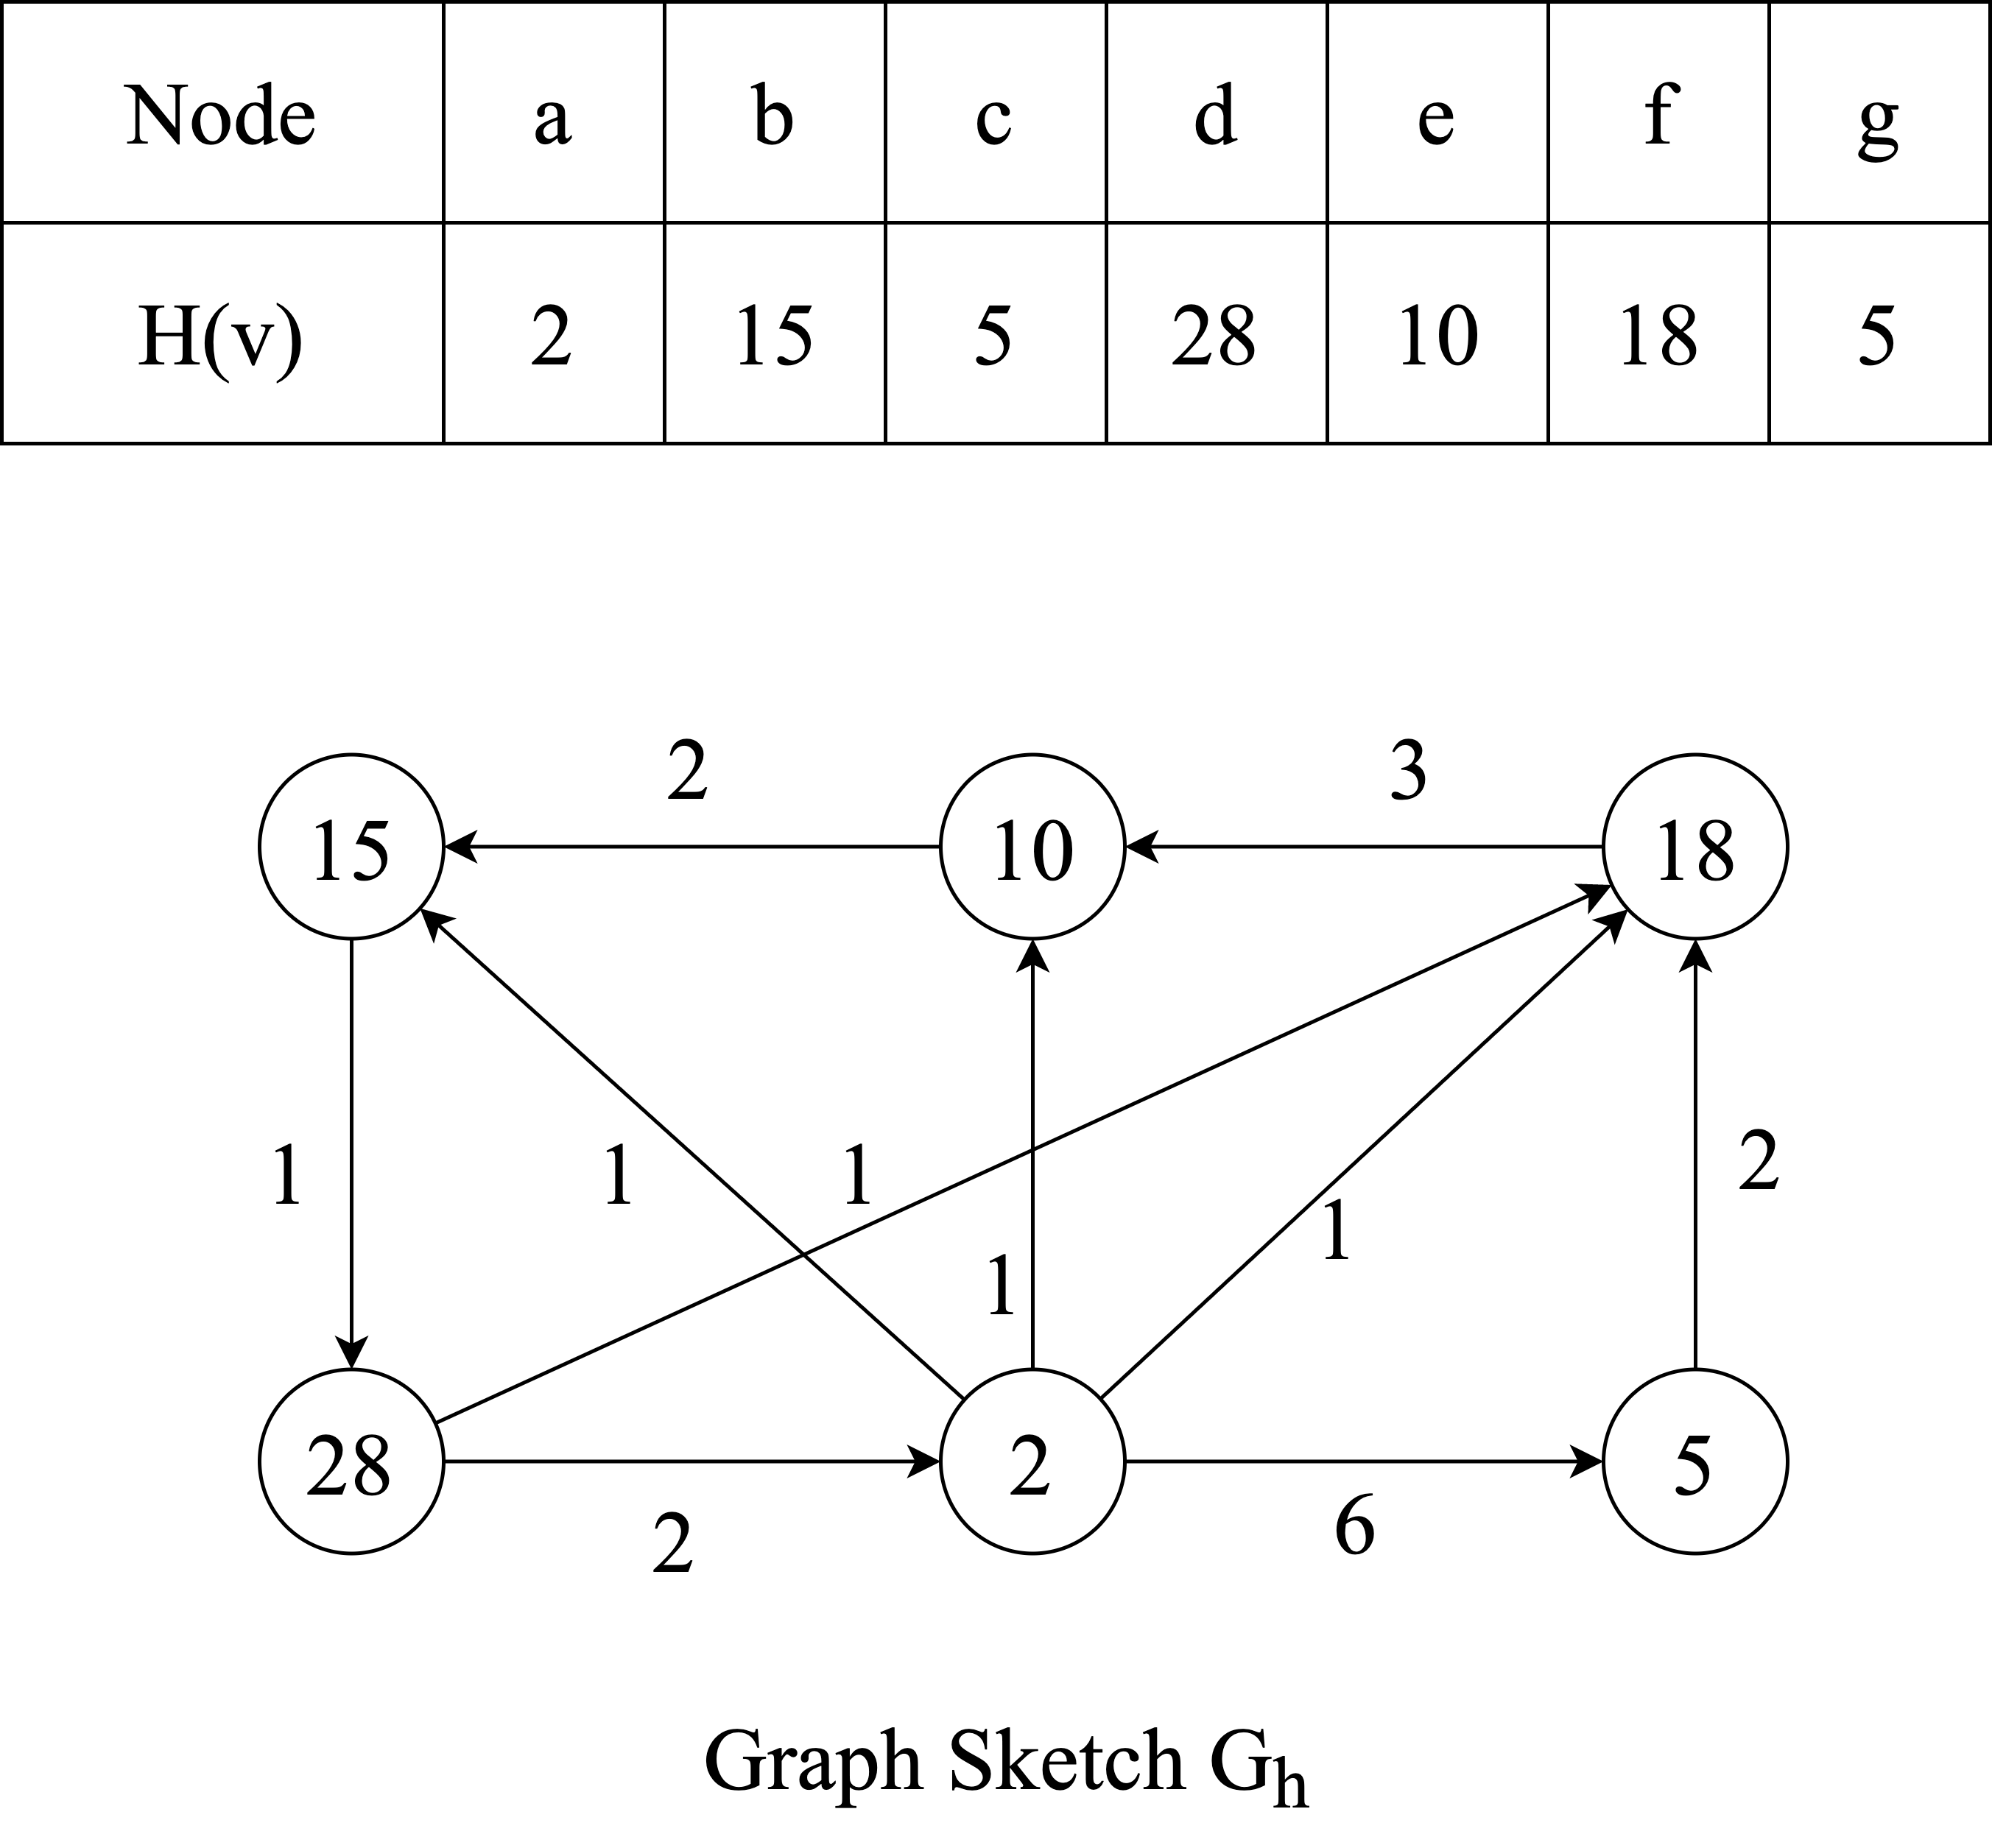
\includegraphics[width=0.6\textwidth]{gss1}
    \caption{A sample map function\cite{gou_fast_2018}}
    \label{fig:gss1}
\end{figure}

\paragraph{}
\(H(.)\) is a hash function which is used on the vertices of the original graph stream to create the graph sketch \(G\textsubscript{h}\) as indicated in Figure \ref{fig:gss1}.

\paragraph{}
A GSS sketch consists of two parts,

\begin{enumerate}
    \item Adjacency matrix
    \item List buffer B for leftover edges
\end{enumerate}

\paragraph{}
For each node in the sketch graph \(G\textsubscript{h}\), an address \(h(v)\) and a fingerprint \(f(v)\) is defined. Each edge \(H(s)\), \(H(d)\) is mapped into a bucket in the row \(h(s)\), column \(h(d)\) of the matrix. \([\langle f(s), f(d)\rangle, w]\) is recorded in the corresponding bucket of the matrix, where \(w\) is the edge weight and \(f(s)\), \(f(d)\) are the fingerprints for the source and destination. This can be seen in the sample of GSS sketch shown in Figure \ref{fig:gss2}.

\begin{figure}[H]
    \centering
    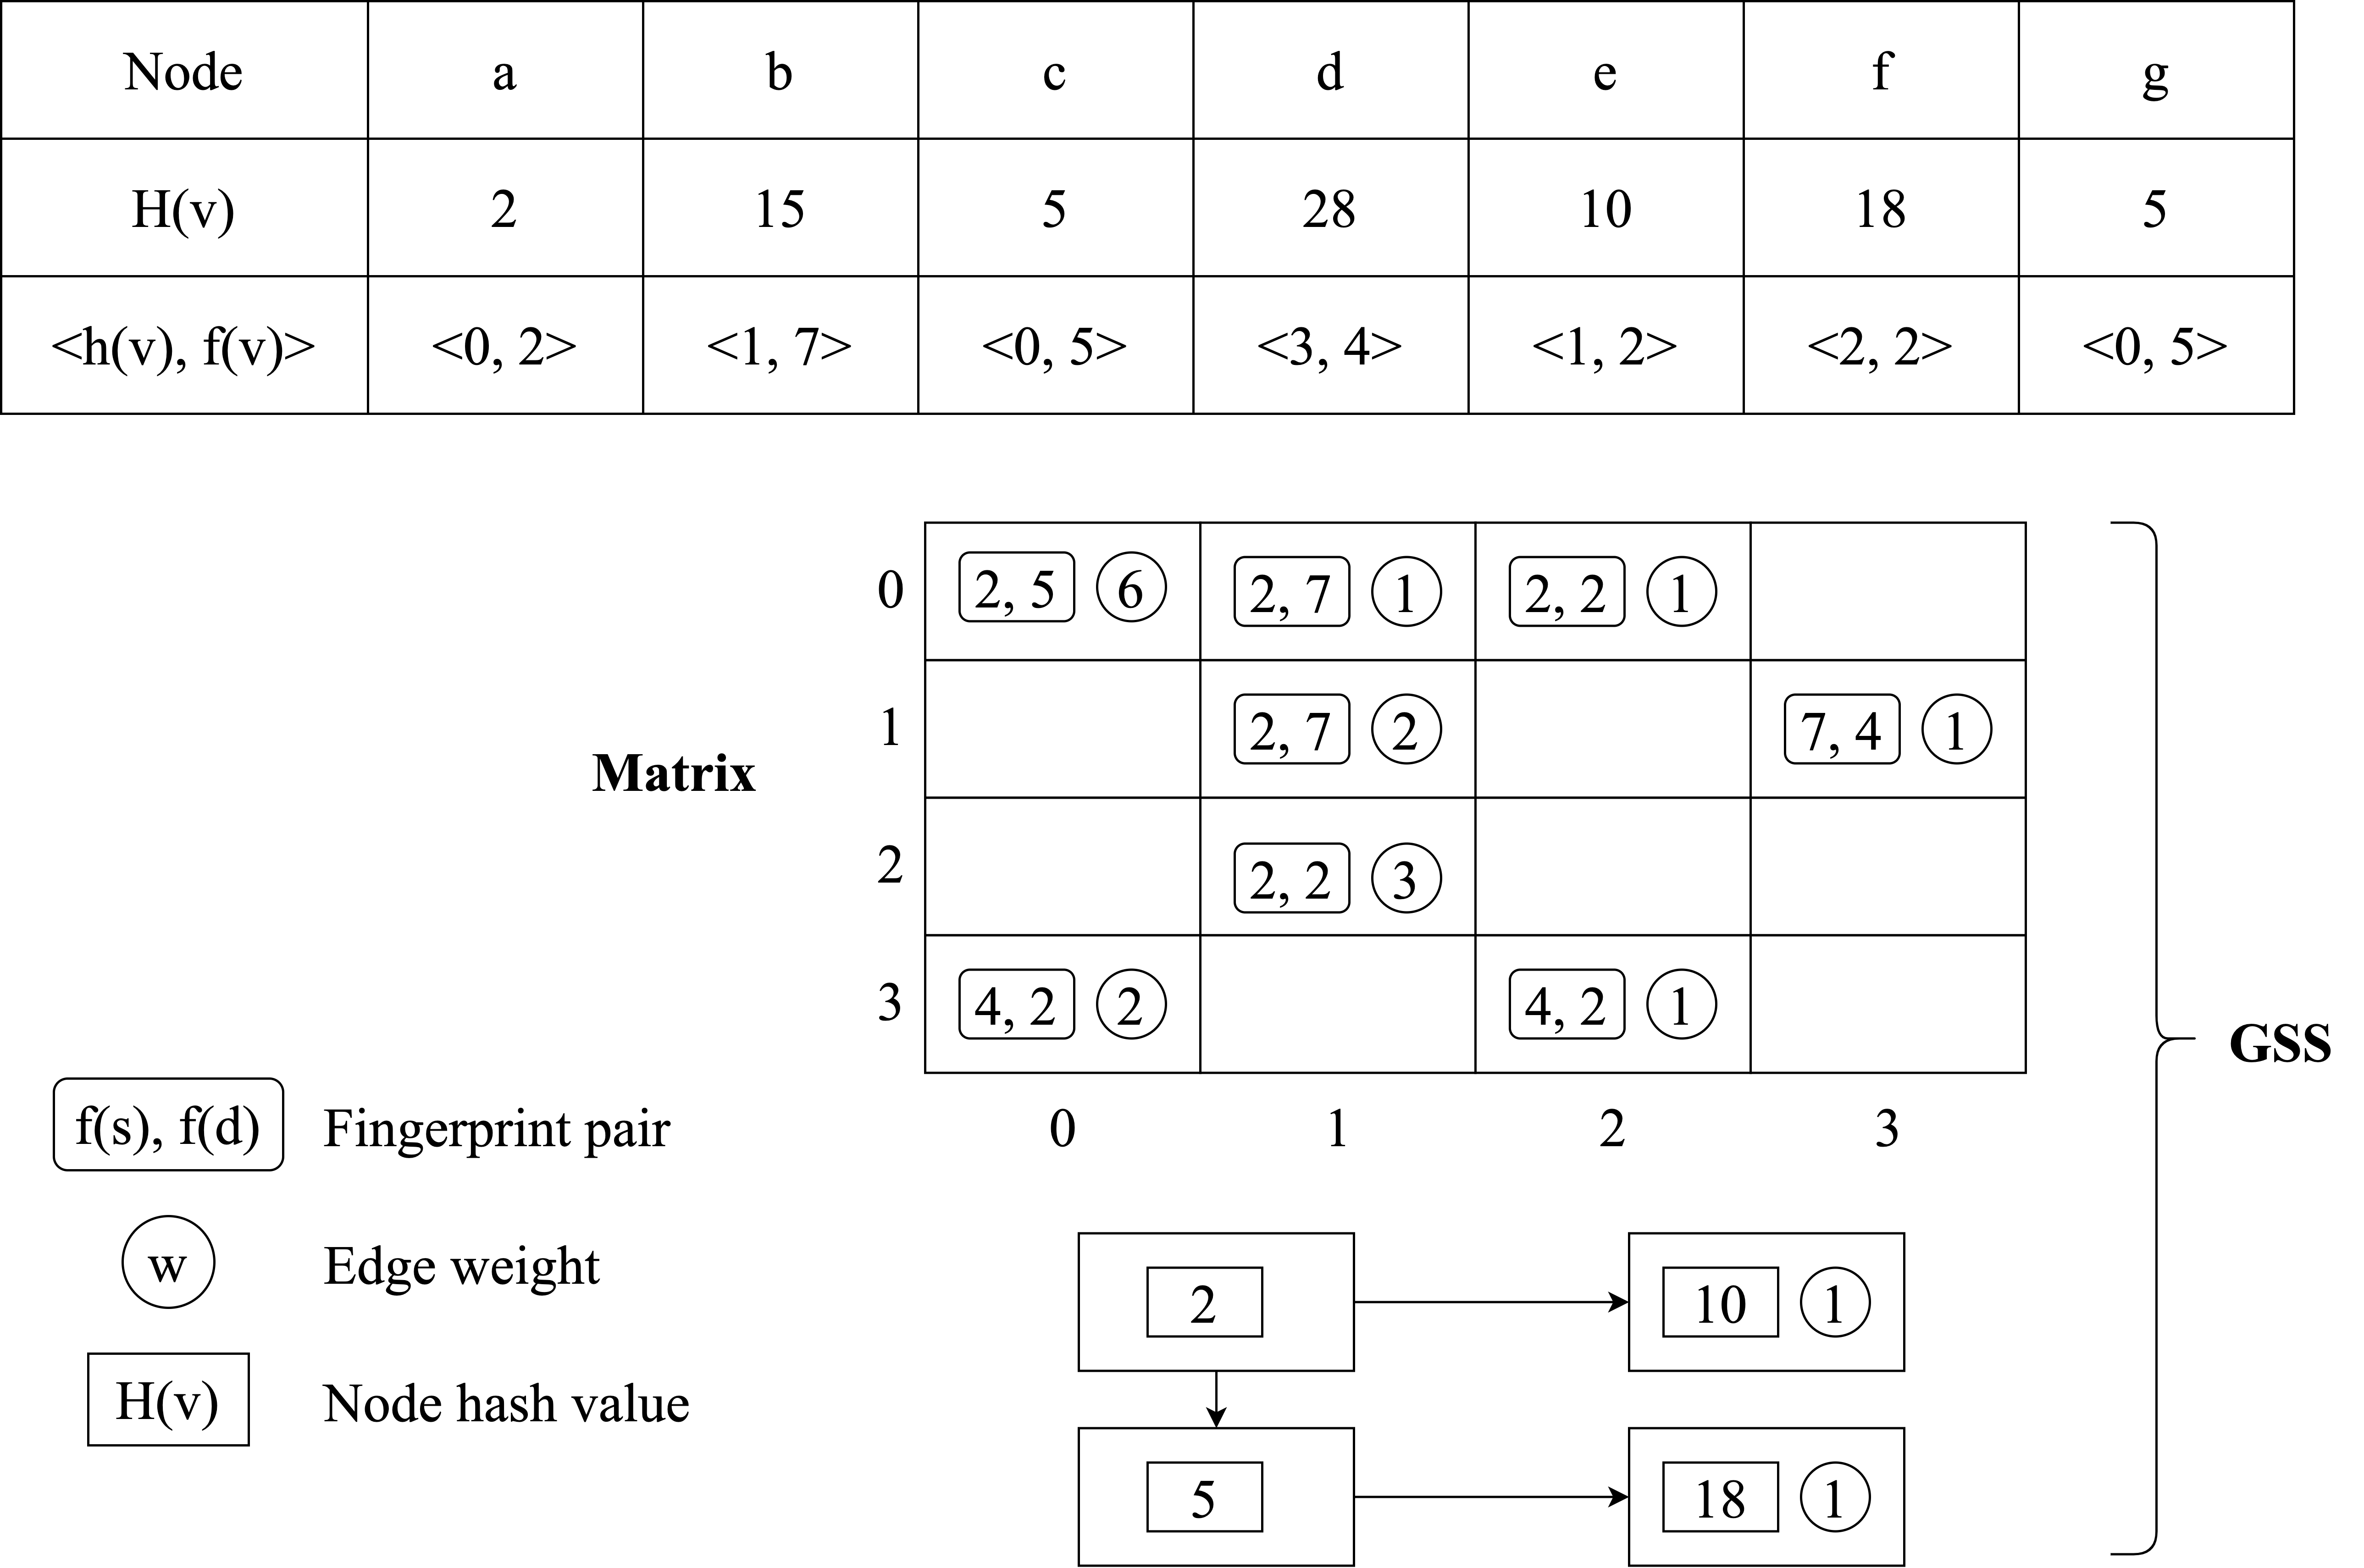
\includegraphics[width=\textwidth]{gss2}
    \caption{A sample version of the basic data structure\cite{gou_fast_2018}}
    \label{fig:gss2}
\end{figure}
\section{Summary}

\paragraph{}
This chapter gives an introduction to the most relevant related work for this research. Throughout this chapter, the representations of graphs in computers, real world graphs, graph summarization had been explained giving much focus to streaming graph summarization. The dissertation will address the research design in the next chapter.
\chapter{Design}
\label{section:design}

\section{Introduction}

Massive-scale datasets are becoming increasingly common today. The growth of the number of users who are actively using digital devices connected to the internet has vastly affected this phenomenon. Also, there lies an interest in researchers to solve the problems which involve large datasets. Most of these datasets could be mapped into graphs to extract useful information, giving rise to the need for processing massive scale graphs. There are many practical scenarios where massive scale graphs are applied such as social networks, network traffic data, and road networks.

It is much easier to work with graphs when they are static and small. However, most of the natural graphs that are being encountered in the real world are dynamic. It becomes increasingly complex to handle the graph as the velocity with which its edges get updated increases. Large scale dynamic natural graphs are used by many companies today. Google uses the PageRank algorithm\cite{brin_anatomy_1998, page_pagerank_nodate} to map the links between the web pages. Facebook has a massive graph with trillions of edges\cite{ching_one_2015}, depicting the interactions of each user on the platform.

With the size of the massive scale graphs, it is difficult to evaluate their properties even after partitioning into multiple nodes. The graphs have to be summarized so that important information regarding the underlying dataset can be inferred easily.

Being applied in a wide range of industrial and research applications, realtime property evaluation of streaming and dynamic natural graphs is a critical requirement in many scenarios. Graph summarization plays a significant role in this as it reduces the computational resources required to evaluate the properties in a rather massive scale streaming graph. It would be beneficial for many sectors if the process of summarizing streaming graphs were made efficient.

In this work, we propose an improved streaming graph summarization technique; kMatrix. It can outperform the existing state of the art summarization sketches by efficiently using the available memory to answer the queries more accurately. We also show that kMatrix is generally faster than the other sketches in handling the graph streams. Despite the number of methods that have been devised for streaming graph summarization, they still lack the accuracy to be used in most real-world scenarios\cite{kumarage_efficient_2017}. Our motivation in improving the existing sketching techniques lies in increasing the efficiency of the application domains, such as real-time property evaluation of the social networks where streaming graph summarization is critical. 
\section{Research design}
\label{section:design_research_design}

\paragraph{}
\autoref{fig:research_design} shows the high level architecture of this research. It depicts the stepwise procedure in reaching the conclusion of the research. It has been broken down into 10 major steps.

\begin{figure}
    \centering 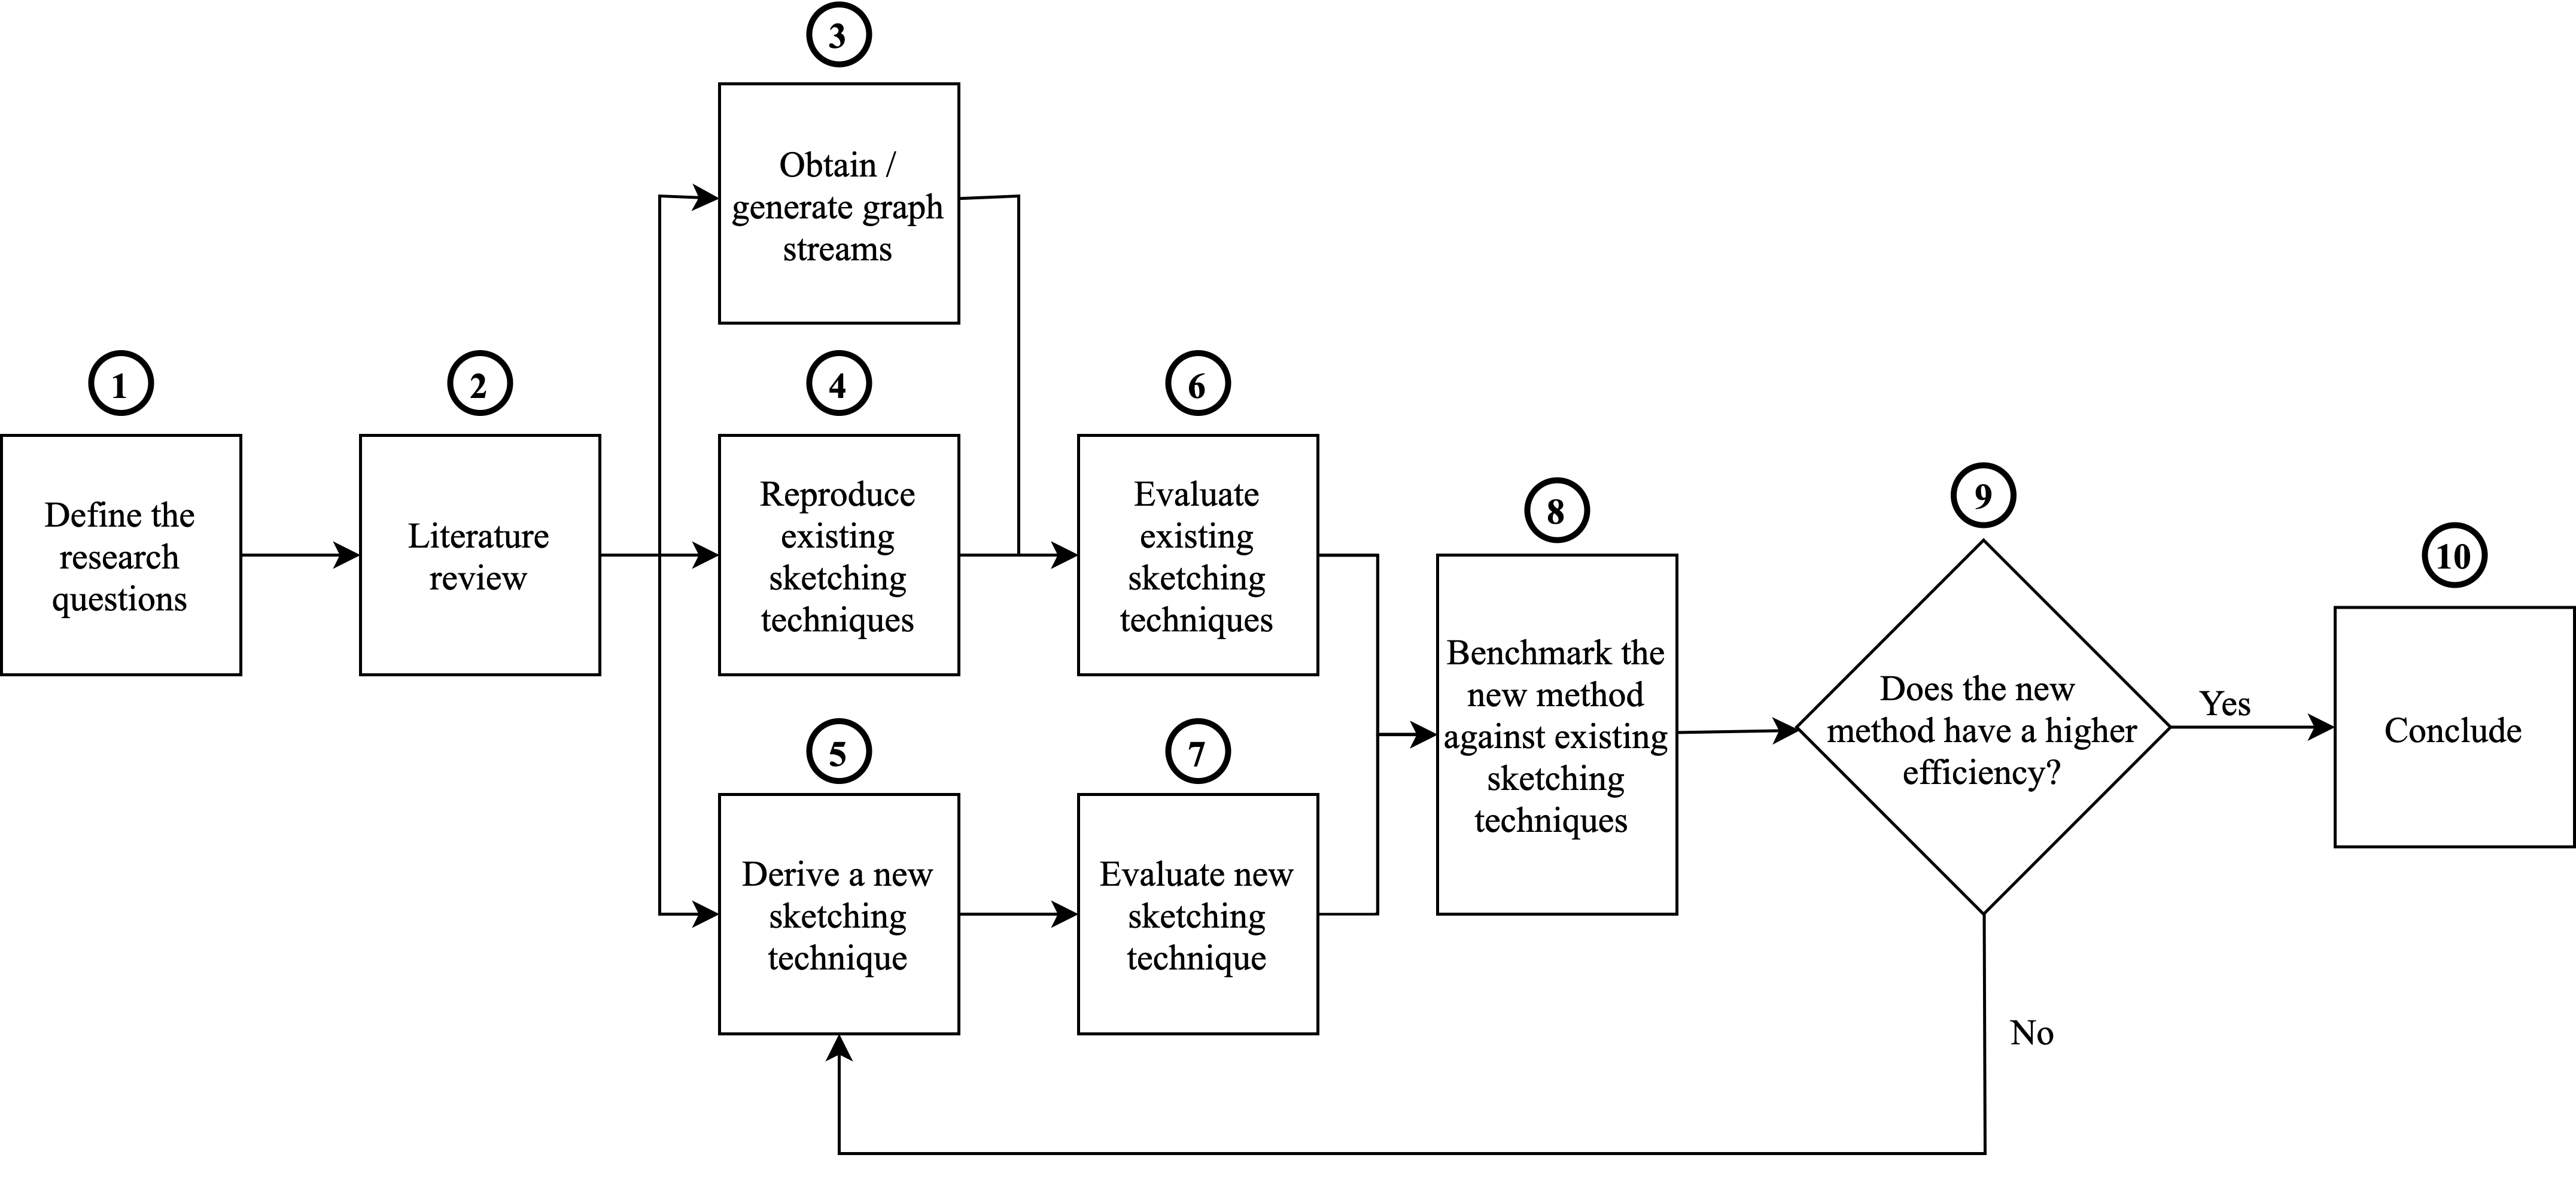
\includegraphics[width=\textwidth]{research_design}
    \caption{High level architecture of the research design}
    \label{fig:research_design}
\end{figure}

\subsection*{Step 1 - Define the research question}

\paragraph{}
Our research questions are,

\begin{enumerate}
    \item What are the tradeoffs of existing graph summarization techniques?
    \item How to improve upon existing streaming graph summarization sketches in order to increase the accuracy of the queries answered through these sketches?
\end{enumerate}

\paragraph{}
In order to achieve this, a comprehensive literature review on the existing streaming graph sketching techniques would have to be done. This will be done in step 2.

\subsection*{Step 2 - Literature review}

\paragraph{}
In this step a literature review will be done on the following areas,

\begin{itemize}
    \item Streaming graphs
    \item Graph sketches and synopses
    \item Graph partitioning
    \item Graph summarization
          \begin{itemize}
              \item General stream summarization techniques
          \end{itemize}
    \item Graph properties
          \begin{itemize}
              \item Real world graph properties
          \end{itemize}
\end{itemize}

\paragraph{}
All the graph summarization techniques that are relevant for this research will be studied in depth.

\subsection*{Step 3 - Obtain / generate graph streams}

\paragraph{}
Step 3 will consist of obtaining datasets for the purpose of testing and benchmarking the implementations. Since this research is geared towards general queries, datasets will have to be chosen from different application domains.

\subsection*{Step 4 - Reproduce existing sketching techniques}

\paragraph{}
Existing sketching techniques will be re-implemented. This step is necessary as query results with the results obtained from the proposed sketching technique will have to be compared in order to deduce the strengths and weaknesses of the proposed method.

\subsection*{Step 5 - Derive a new sketching technique}

\paragraph{}
In step 5, a new sketching technique will be proposed and implemented after studying all the relevant existing work (step 2).

\paragraph{}
In addition to implementing the proposed method, its properties and boundaries will be deduced in mathematical form. Theoretical proofs will be devised in order to prove the generalizability of the proposed technique.

\subsection*{Step 6 - Evaluate existing sketching techniques}

\paragraph{}
Implemented existing sketching techniques will be benchmarked against selected datasets and the results will be obtained.

\subsection*{Step 7 - Evaluate new sketching technique}

\paragraph{}
Proposed sketching technique will be benchmarked against selected datasets and the results will be obtained.

\subsection*{Step 8 - Benchmark the new method against existing sketching techniques}

\paragraph{}
In step 8, the results obtained from step 6 and step 7 will be compared to multiple characteristics.

\paragraph{}
Examples for some evaluation measures are,

\begin{itemize}
    \item Average relative error\cite{zhao_gsketch:_2011}
    \item Number of effective queries\cite{zhao_gsketch:_2011}
\end{itemize}

Examples for some of the comparisons are,

\begin{itemize}
    \item Compression ratio vs Average relative error
    \item Number of hash functions vs Average relative error
\end{itemize}

\subsection*{Step 9 - Does the new method have a higher efficiency?}

\paragraph{}
In this step it will be decided whether the newly proposed sketching technique poses considerable accuracy increase or other advantages over the existing techniques. If it does, the process will move step 10. Otherwise the process would move back to step 5 and iterate the same process.

\subsection*{Step 10 - Conclude}

\paragraph{}
The research will be concluded with detailing down the characteristics of newly proposed streaming graph summarization technique. The conclusion will also contain a mathematical breakdown of the proposed algorithm and its boundaries.
\section{Sources of data}
\label{section:design_sources_of_data}

\paragraph{}
Real-world graph streams had to be used in order to benchmark the sketching algorithms against each other.  The process of finding and preprocessing datasets will be addressed in \autoref{section:sod_datasets} and \autoref{section:soc_preprocessing} respectively.

\subsection{Datasets}
\label{section:sod_datasets}

\paragraph{}
5 datasets were chosen to carry out the benchmarking tests in this research. These were chosen to represent different application domains. The chosen datasets are as follows.

\subsubsection{unicorn-wget\cite{DVN/5H4TDI_2018}}

\paragraph{}
unicorn-wget is a dataset created from capturing the packet information of the network activity of a simulated network. Experiments were run for over an hour, with recurrent wget commands issued throughout the experiments (one for every 120 seconds). This dataset was created at Harvard University and consist of 5 parts.

\begin{enumerate}
    \item Hour-Long Wget Benign Dataset (Base Graph)
    \item Hour-Long Wget Benign Dataset (Streaming Graph)
    \item Hour-Long Wget Attack Dataset (Base Graph)
    \item Hour-Long Wget Attack Dataset (Streaming Graph)
    \item Hour-Long Wget Attack Dataset (Raw)
\end{enumerate}

\paragraph{}
Hour-Long Wget Benign Dataset (Base Graph) which consist of 17,778 nodes and 2,779,726 edges was choosen for the experiment. From this 10\% of the edges were chosen using the reservoir sampling in order to minimize the running time of the sketching algorithms.

\subsubsection{email-EuAll\cite{leskovec_graph_2007}}

\paragraph{}
The network was generated using email data from a large European research institution. The dataset consist of the emails sent out in a period of 18 months. The dataset contains sender, receiver and the time of origination of each email. Given a set of email messages, each node corresponds to an email address. A directed edge has been created between nodes i and j, if i sent at least one message to j. This dataset consist of 265,214 nodes and 420,045 edges\cite{noauthor_snap_nodate_email}.

\subsubsection{cit-HepPh\cite{leskovec_graphs_2005, gehrke_overview_2003}}

\paragraph{}
cit-HepPh (high energy physics phenomenology) citation graph is from the e-print arXiv. It has 34,546 papers (nodes) and 421,578 citations (edges). If a paper i cites paper j, the graph contains a directed edge from i to j\cite{noauthor_snap_nodate_hep}.

\subsubsection{gen-scale-free}

\paragraph{}
This is a randomly generated dataset which obeys the power-law distribution. gen-scale-free contains 100,000 nodes and 400,000 edges. This dataset is generated according to the work, ‘The Degree Sequence of a Scale-Free Random Graph Process’
\cite{bollobas_degree_2001}.

\subsubsection{gen-small-world}

\paragraph{}
This is a randomly generated dataset which has the small-world property. gen-small-world contains 100,000 nodes and 199,997 edges. This dataset is generated according to the work, ‘Random pseudofractal scale-free networks with small-world effect’\cite{wang_random_2006}.

\subsection{Data preprocessing}
\label{section:soc_preprocessing}

\paragraph{}
Each dataset was preprocessed using a Python script. The script is available in appendix \ref{appendix:preprocessor}. A graph data stream is usually represented by its list of edges. The original dataset was preprocessed in a way such that the output only contained a list of \lbrack source\_id, target\_id\rbrack\space which described the edges of the graph.

\paragraph{}
Each dataset was stored in our own private server so that the preprocessor could download the graph stream on the fly and convert it to the appropriate format.
\section{Experiments}
\label{section:design_experiments}

\paragraph{}
Experiments will be carried out on following aspects of the graph streams for the sketching algorithms, CountMin, gSketch, TCM and GMatrix using the selected datasets.

\begin{enumerate}
    \item Build-time test
    \item Average Relative Error of edge queries
    \item Number of Effective Queries
    \item k-Top heavy nodes
    \item k-Top heavy edges
    \item Degree distribution
    \item Edge-weight distribution
    \item Edge insertion time
\end{enumerate}
\section{Evaluation metrics}
\label{section:design_evaluation_metrics}

\subsection{Average relative error}
\label{section:metrics_are}

\paragraph{}
The average relative error is defined as,

\begin{equation}
    er(Q) =  \frac{\tilde{f}'(Q) - f(Q)}{f(Q)} = \frac{\tilde{f}'(Q)}{f(Q)} -1
\end{equation}

\paragraph{}
Given a set of m queries, $\{ Q_1 , ....., Q_m \}$, the average relative error is defined by averaging the relative errors over all queries $Q_i$ for \(i \in [1,m]\) as,

\begin{equation}
    e(Q) =  \frac{\sum_{i=1}^{k} er(Q_i)}{m}
\end{equation}

\subsection{Number of effective queries}
\label{section:metrics_neq}

\paragraph{}
A query is said to be effective if the error, $\tilde{f}'(Q) - f(Q), < G_0$,  where $G_0$ is a predefined value. The number of effective queries is defined as,

\begin{equation}
    g(Q) =  \left | \{\,q\, |   \left |\tilde{f}'(q) - f(q)\right | \leq G_0, \,q \, \epsilon  \,Q\} \, \right|
\end{equation}

This can also be expressed as a percentage of effective queries as,

\begin{equation}
    g(Q) =  \frac{\left | \{\,q\, |   \left |\tilde{f}'(q) - f(q)\right | \leq G_0, \,q \, \epsilon  \,Q\} \, \right|}{|Q|}*100
\end{equation}

\subsection{Intersection accuracy}
\label{section:metrics_inter}

\paragraph{}
The results for the top-k heavy nodes and edges in \autoref{section:heavy_nodes} and \autoref{section:heavy_edges} will be evaluated using an intersection metric\cite{fagin_comparing_2003}. If X is the top-k results generated through the sketch and Y is the top-k results generated through the original stream, the inter accuracy is defined as \(|X \cap Y|/k\). The range of inter-accuracy is between 0 and 1 where 1 is resulted when all the k items being matched and 0 is resulted when none of the items matched.
\section{Summary}

\paragraph{}
This chapter gives an introduction to the most relevant related work for this research. Throughout this chapter, the representations of graphs in computers, real world graphs, graph summarization had been explained giving much focus to streaming graph summarization. The dissertation will address the research design in the next chapter.
\chapter{Implementation}
\label{section:implementation}

\section{Introduction}

Massive-scale datasets are becoming increasingly common today. The growth of the number of users who are actively using digital devices connected to the internet has vastly affected this phenomenon. Also, there lies an interest in researchers to solve the problems which involve large datasets. Most of these datasets could be mapped into graphs to extract useful information, giving rise to the need for processing massive scale graphs. There are many practical scenarios where massive scale graphs are applied such as social networks, network traffic data, and road networks.

It is much easier to work with graphs when they are static and small. However, most of the natural graphs that are being encountered in the real world are dynamic. It becomes increasingly complex to handle the graph as the velocity with which its edges get updated increases. Large scale dynamic natural graphs are used by many companies today. Google uses the PageRank algorithm\cite{brin_anatomy_1998, page_pagerank_nodate} to map the links between the web pages. Facebook has a massive graph with trillions of edges\cite{ching_one_2015}, depicting the interactions of each user on the platform.

With the size of the massive scale graphs, it is difficult to evaluate their properties even after partitioning into multiple nodes. The graphs have to be summarized so that important information regarding the underlying dataset can be inferred easily.

Being applied in a wide range of industrial and research applications, realtime property evaluation of streaming and dynamic natural graphs is a critical requirement in many scenarios. Graph summarization plays a significant role in this as it reduces the computational resources required to evaluate the properties in a rather massive scale streaming graph. It would be beneficial for many sectors if the process of summarizing streaming graphs were made efficient.

In this work, we propose an improved streaming graph summarization technique; kMatrix. It can outperform the existing state of the art summarization sketches by efficiently using the available memory to answer the queries more accurately. We also show that kMatrix is generally faster than the other sketches in handling the graph streams. Despite the number of methods that have been devised for streaming graph summarization, they still lack the accuracy to be used in most real-world scenarios\cite{kumarage_efficient_2017}. Our motivation in improving the existing sketching techniques lies in increasing the efficiency of the application domains, such as real-time property evaluation of the social networks where streaming graph summarization is critical. 
\section{Implementation of the test suite}
\label{section:test_suite}

\subsection{Core architecture}

\paragraph{}
The architecture of the benchmarking test suit is designed in a rather simple manner such that it permits easy addition of more test cases or graph sketches. It is shown in \autoref{fig:test_suite}.

\begin{figure}[H]
    \centering 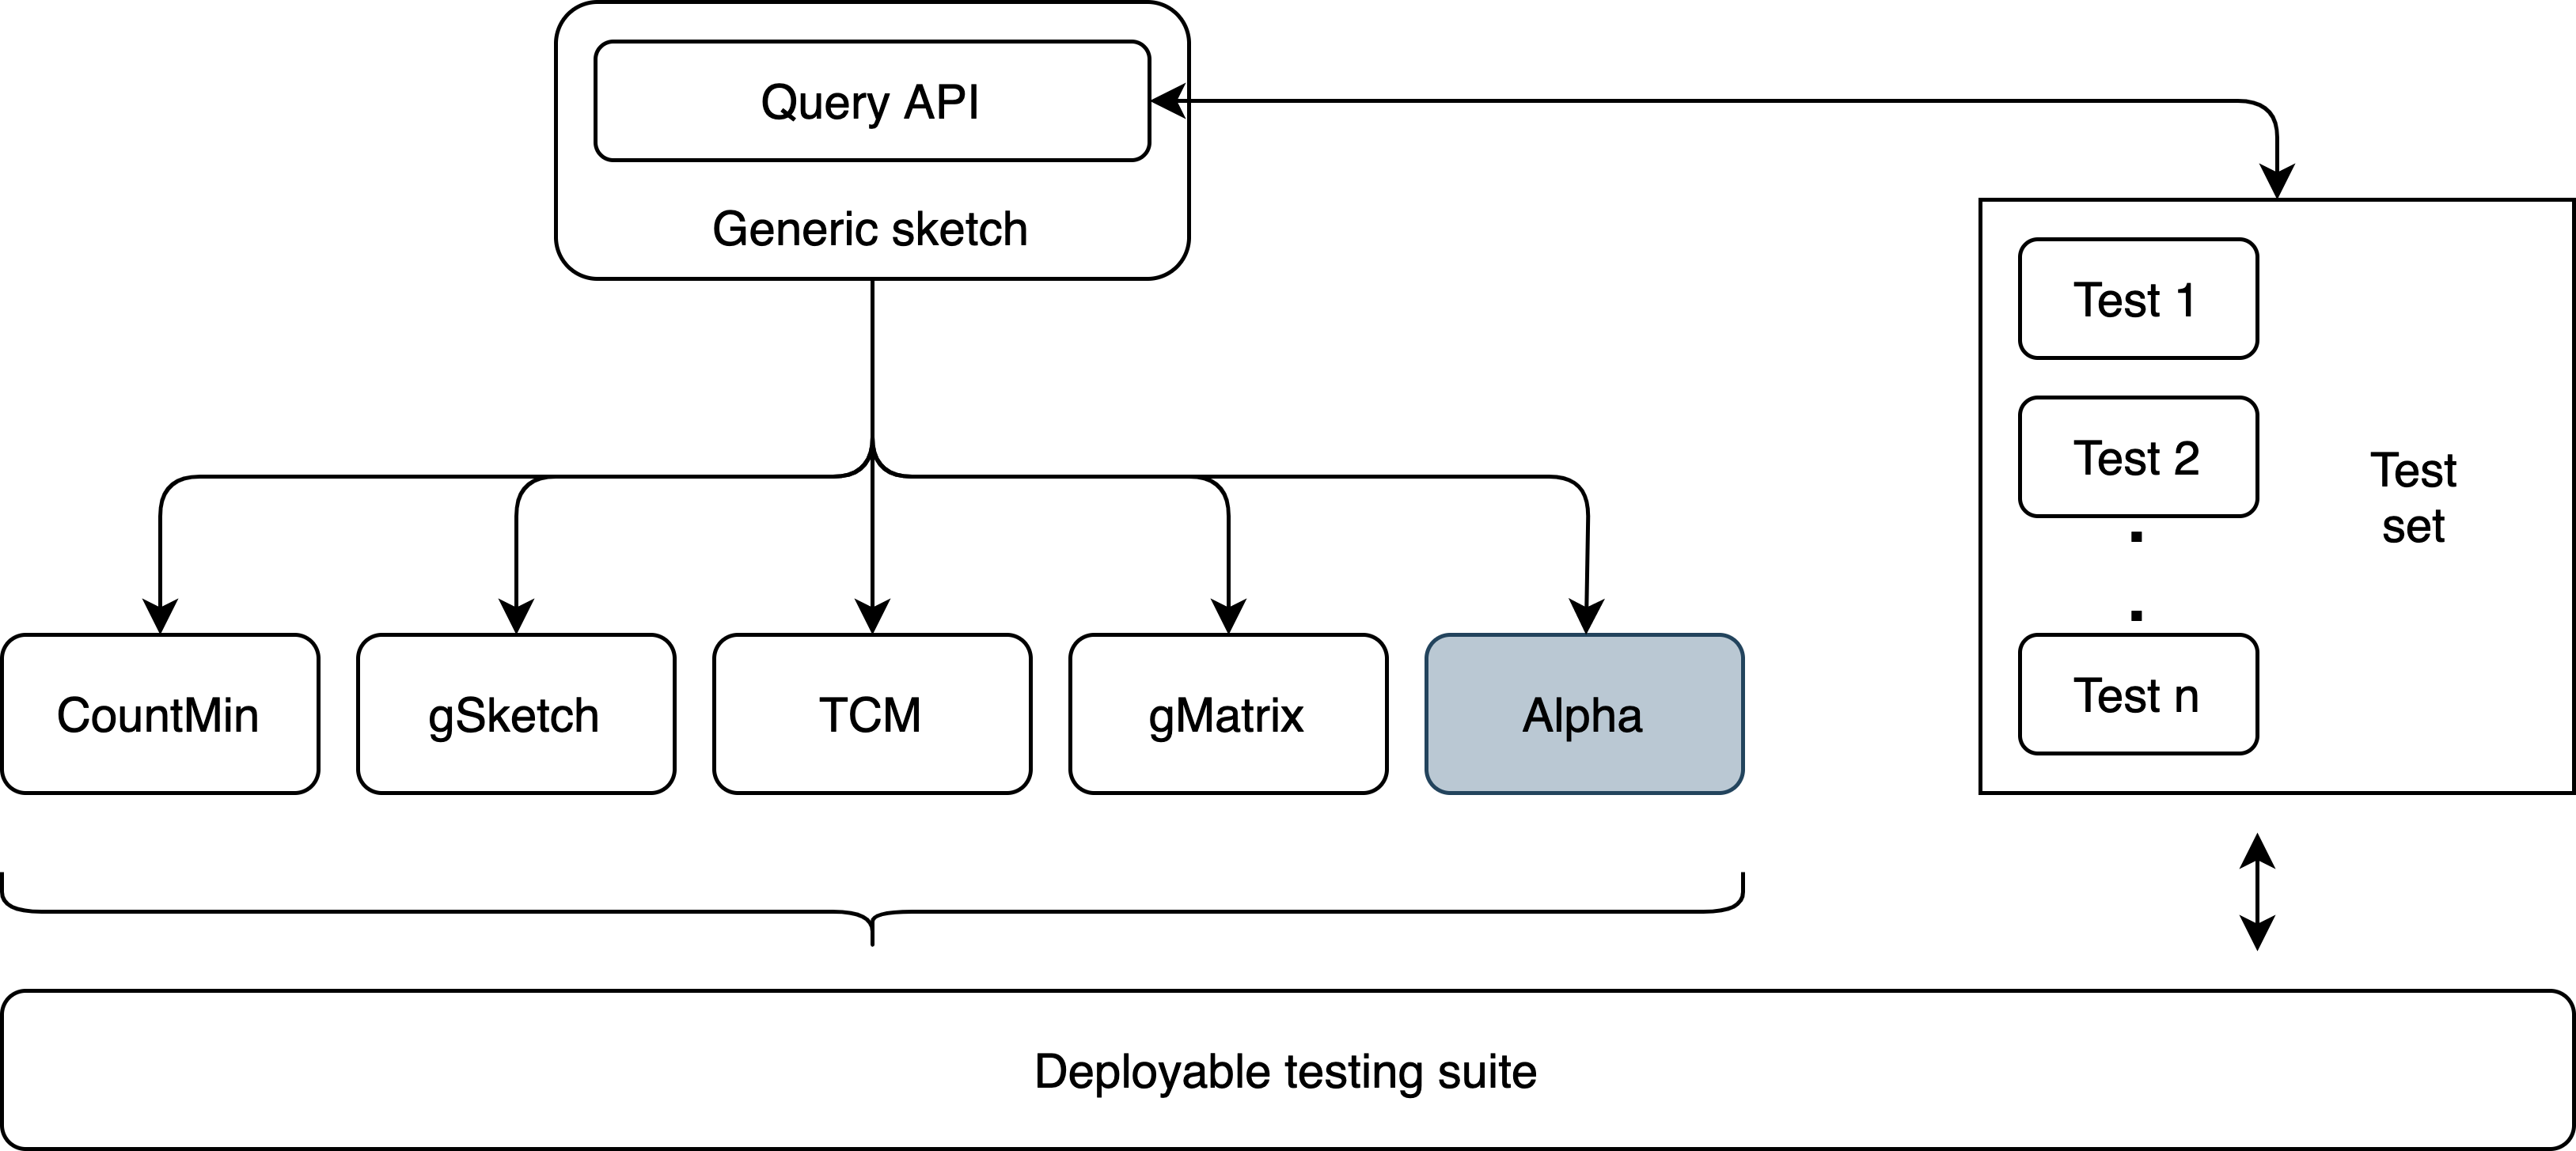
\includegraphics[width=\textwidth]{test_suite}
    \caption{High level architecture of the test suite}
    \label{fig:test_suite}
\end{figure}

\paragraph{}
All the sketches are extended from a generic ‘Sketch’ class which allows the tests to retrieve information through a same interface. This class contains the abstract methods \textbf{add\_edge{()}}, \textbf{get\_edge\_frequency{()}} and \textbf{print\_analytics{()}}. They were to be implemented by any of the sketches that inherit from the base Sketch class. The code for the base Sketch class is depicted in \autoref{lst:sketch}.\\

\pythonexternal[caption={Sketch class}, label={lst:sketch}]{code_listings/sketch.py}

\subsection{Utility functions}

\paragraph{}
All the utility functions were implemented in a separate Python module. The reservoir sampling of data streams was done using the sampling function depicted in \autoref{lst:sampling}.

\pythonexternal[caption={Reservoir sampling function}, label={lst:sampling}]{code_listings/sampling.py}

\paragraph{}
The \textbf{timeit} function used for the timing of code sections can be found in the appendix \ref{appendix:timeit}.

\subsection{Summarization sketches}

\paragraph{}
Restating the aforementioned, all the summarization sketches have been extended from the base Sketch class. The implementation code for the sketches, CountMin, gSketch, TCM and GMatrix can be found respectively in \ref{appendix:countmin}, \ref{appendix:gsketch}, \ref{appendix:tcm} and \ref{appendix:gmatrix} appendix sections.
\section{Implementation of Alpha}

\paragraph{}
The Alpha sketch is an improvement over the GMatrix algorithm. The idea behind the Alpha sketch is simple. It partitions the frequency matrix of the GMtrix sketch according to the partition algorithm proposed in gSketch in order to reduce the average relative error of the queries. This high-level concept of the Alpha is depicted in \autoref{fig:alpha}. The method proposed to reduce the average relative error is to recursively partition the available amount of memory according to a sample of the original graph stream. More details about the partitioning technique of gSketch will be discussed in \autoref{section:gsketch_partitioning}.

\begin{figure}[H]
    \centering 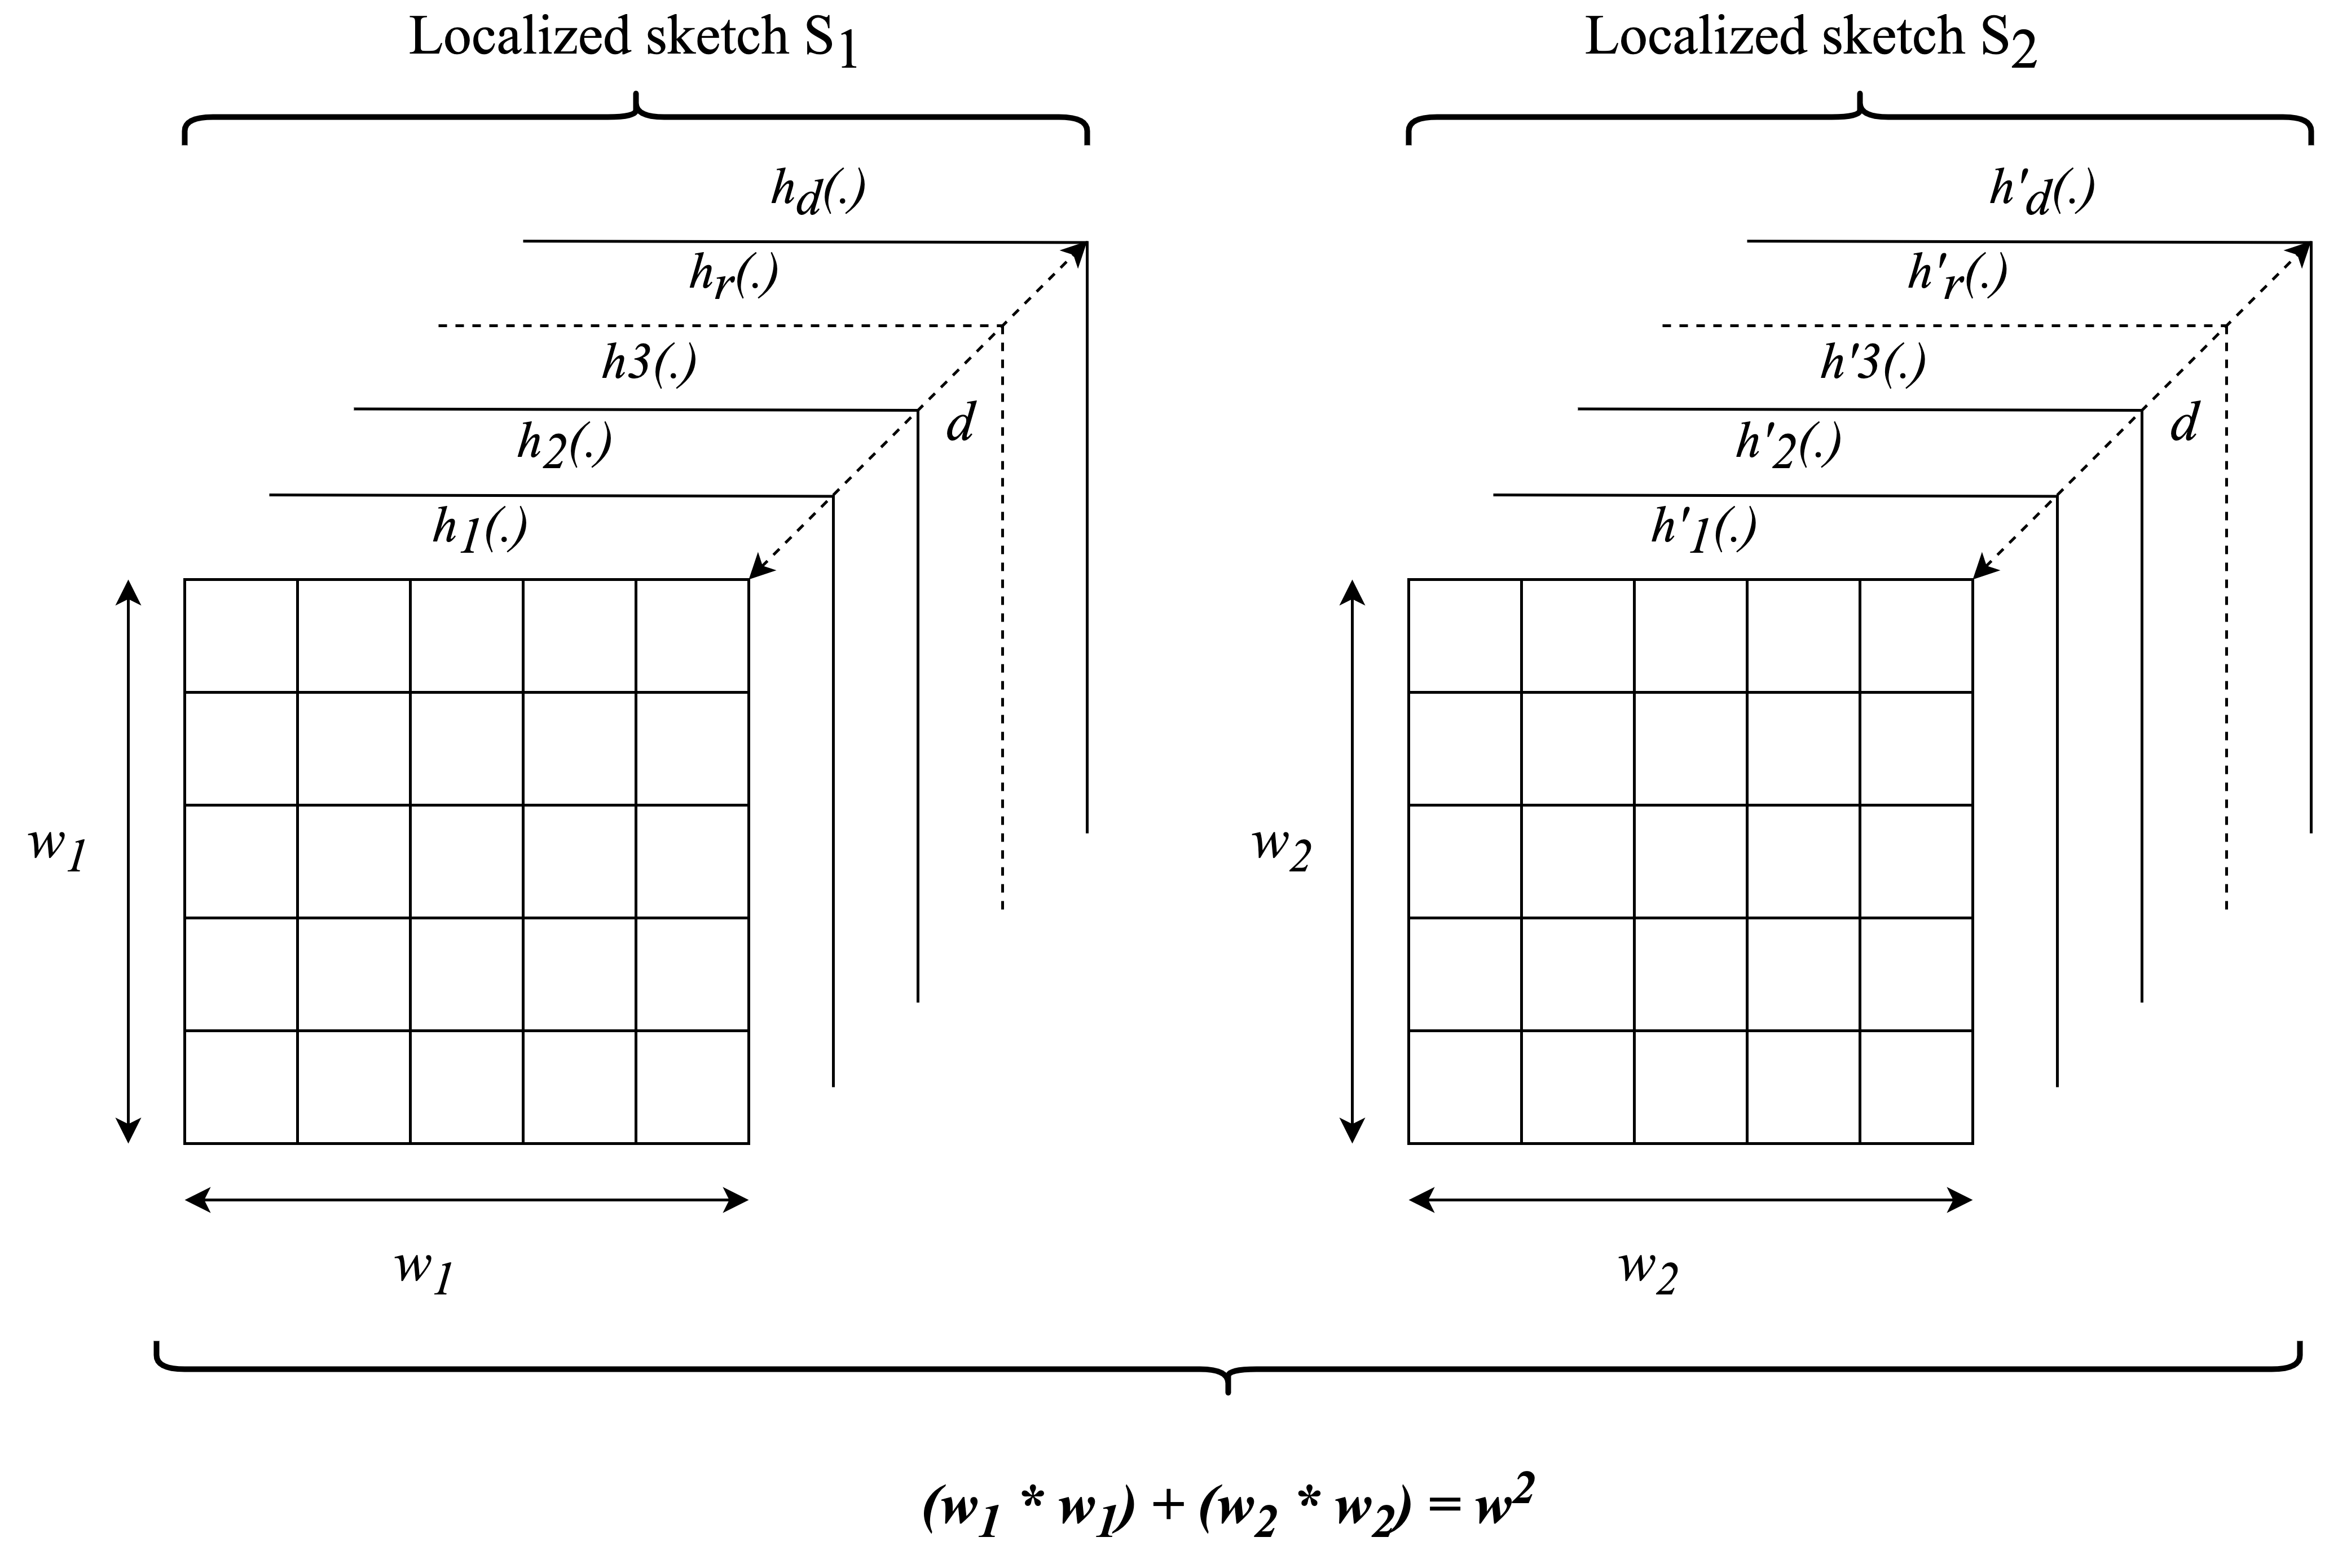
\includegraphics[width=\textwidth]{alpha}
    \caption{High level concept of Alpha sketch}
    \label{fig:alpha}
\end{figure}

\paragraph{}
The implementation code for alpha can be found in the appendix \autoref{appendix:alpha}.

\subsection{Partitioning algorithm in gSketch\cite{zhao_gsketch:_2011}}
\label{section:gsketch_partitioning}

\paragraph{}
A summarized version of the underlying theory and the algorithm is discussed in this section. The complete sketch partitioning process is given in the original gSketch paper.

\paragraph{}
Consider that the original sketch is partitioned into i sub-sketches. Let \(F(S_i)\) is the sum of the edge frequencies in the \(i\)th sketch. If \((m,n)\) is an edge in the \(i\)th sketch, let \(\bar{f}(m,n)\) be its expected frequency. Then,

\[\bar{f}(m,n) = (F(S_i) - f(m,n)) / w_i\]

\paragraph{}
Then the expected relative error of \((m,n)\) is given by,

\begin{equation}
    \bar{e}(m,n) = \bar{f}(m,n) / f(m,n) = F(S_i) / (f(m,n) . w_i) - 1 / w_i
    \label{eq:1}
\end{equation}

\paragraph{}
Then the overall relative error \(E_i\) of the sketch can be expressed as,

\begin{equation}
    \sum_{(m,n) \in S_i}^{} \bar{e}(m,n)
    \label{eq:2}
\end{equation}

\paragraph{}
Let the average frequency of a vertex be \(\tilde{f}_v(m)\) and the estimated out-degree of the \(m\) be \(\tilde{d}(m)\). Then the average frequency of the vertex would be \( \tilde{f}_v(m) / \tilde{d}(m) \). And the total estimated frequencies of the partitioned sketch \(S_i\) can be expressed as,

\begin{equation}
    \tilde{F}(S_i) = \sum_{m \in S_i \: ; \: m \in V}^{} \tilde{f}_v(m)
    \label{eq:3}
\end{equation}

\paragraph{}
According to the \autoref{eq:1}, \autoref{eq:2} and \autoref{eq:3},

\begin{equation}
    E_i = \sum_{m \in S_i}^{} \frac{\tilde{d}(m) . \tilde{F}(S_i)}{w_i . (\tilde{f}_v(m) / \tilde{d}(m))} - \sum_{m \in S_i}^{} \tilde{d}(m) / w_i
    \label{eq:4}
\end{equation}

\paragraph{}
\(\tilde{d}(m)\) in the numerator accounts for the fact that \(O(\tilde{d}(m))\) edges are coming out of the vertex m.

\paragraph{}
When a sketch of width \(w\) is partitioned into two sketches of widths \(w_1\) and \(w_2\), the total error can be expressed as \(E = E_1 + E_2\). Here \(w_1 = w_2\).

\begin{equation}
    E = \sum_{m \in S_1}^{} \frac{\tilde{d}(m) . \tilde{F}(S_i)}{w_1 . (\tilde{f}_v(m) / \tilde{d}(m))} + \sum_{m \in S_2}^{} \frac{\tilde{d}(m) . \tilde{F}(S_i)}{w_2 . (\tilde{f}_v(m) / \tilde{d}(m))} - \sum_{m \in S_1 \cup S_2}^{} \tilde{d}(m) / w_1
    \label{eq:5}
\end{equation}

\paragraph{}
The \autoref{eq:5} can be further simplified as,

\begin{equation}
    E' = E . w_1 + \sum_{m \in S_1 \cup S_2}^{} \tilde{d}(m)
\end{equation}

\paragraph{}
Here the value of \(E'\) is,

\begin{equation}
    E' = \sum_{m \in S_1}^{} \frac{\tilde{d}(m) . \tilde{F}(S_i)}{\tilde{f}_v(m) / \tilde{d}(m)} + \sum_{m \in S_2}^{} \frac{\tilde{d}(m) . \tilde{F}(S_i)}{\tilde{f}_v(m) / \tilde{d}(m)}
    \label{eq:6}
\end{equation}

\paragraph{}
So it is evident that the overall error can be minimized by choosing the smallest \(E'\) according to the \autoref{eq:6}. Therefor the underlying idea behind the partitioning algorithm is to choose a data sample of the original stream and then repeatedly partition the available space between the vertices in the sample according to the \autoref{eq:6}. After this initialization phase, the streaming can begin and the edges that represented the vertices in the sample got to their respective partitioned sketches.
\section{Summary}

\paragraph{}
This chapter gives an introduction to the most relevant related work for this research. Throughout this chapter, the representations of graphs in computers, real world graphs, graph summarization had been explained giving much focus to streaming graph summarization. The dissertation will address the research design in the next chapter.
\chapter{Results and Evaluation}
\label{section:results_n_evaluation}

\section{Introduction}

Massive-scale datasets are becoming increasingly common today. The growth of the number of users who are actively using digital devices connected to the internet has vastly affected this phenomenon. Also, there lies an interest in researchers to solve the problems which involve large datasets. Most of these datasets could be mapped into graphs to extract useful information, giving rise to the need for processing massive scale graphs. There are many practical scenarios where massive scale graphs are applied such as social networks, network traffic data, and road networks.

It is much easier to work with graphs when they are static and small. However, most of the natural graphs that are being encountered in the real world are dynamic. It becomes increasingly complex to handle the graph as the velocity with which its edges get updated increases. Large scale dynamic natural graphs are used by many companies today. Google uses the PageRank algorithm\cite{brin_anatomy_1998, page_pagerank_nodate} to map the links between the web pages. Facebook has a massive graph with trillions of edges\cite{ching_one_2015}, depicting the interactions of each user on the platform.

With the size of the massive scale graphs, it is difficult to evaluate their properties even after partitioning into multiple nodes. The graphs have to be summarized so that important information regarding the underlying dataset can be inferred easily.

Being applied in a wide range of industrial and research applications, realtime property evaluation of streaming and dynamic natural graphs is a critical requirement in many scenarios. Graph summarization plays a significant role in this as it reduces the computational resources required to evaluate the properties in a rather massive scale streaming graph. It would be beneficial for many sectors if the process of summarizing streaming graphs were made efficient.

In this work, we propose an improved streaming graph summarization technique; kMatrix. It can outperform the existing state of the art summarization sketches by efficiently using the available memory to answer the queries more accurately. We also show that kMatrix is generally faster than the other sketches in handling the graph streams. Despite the number of methods that have been devised for streaming graph summarization, they still lack the accuracy to be used in most real-world scenarios\cite{kumarage_efficient_2017}. Our motivation in improving the existing sketching techniques lies in increasing the efficiency of the application domains, such as real-time property evaluation of the social networks where streaming graph summarization is critical. 
\section{Build-time}

\subsection*{Purpose}
To compare the time taken for the creation of each sketch under different types of graph streams.

\subsection*{Results}

\begin{figure}[H]
    \centering 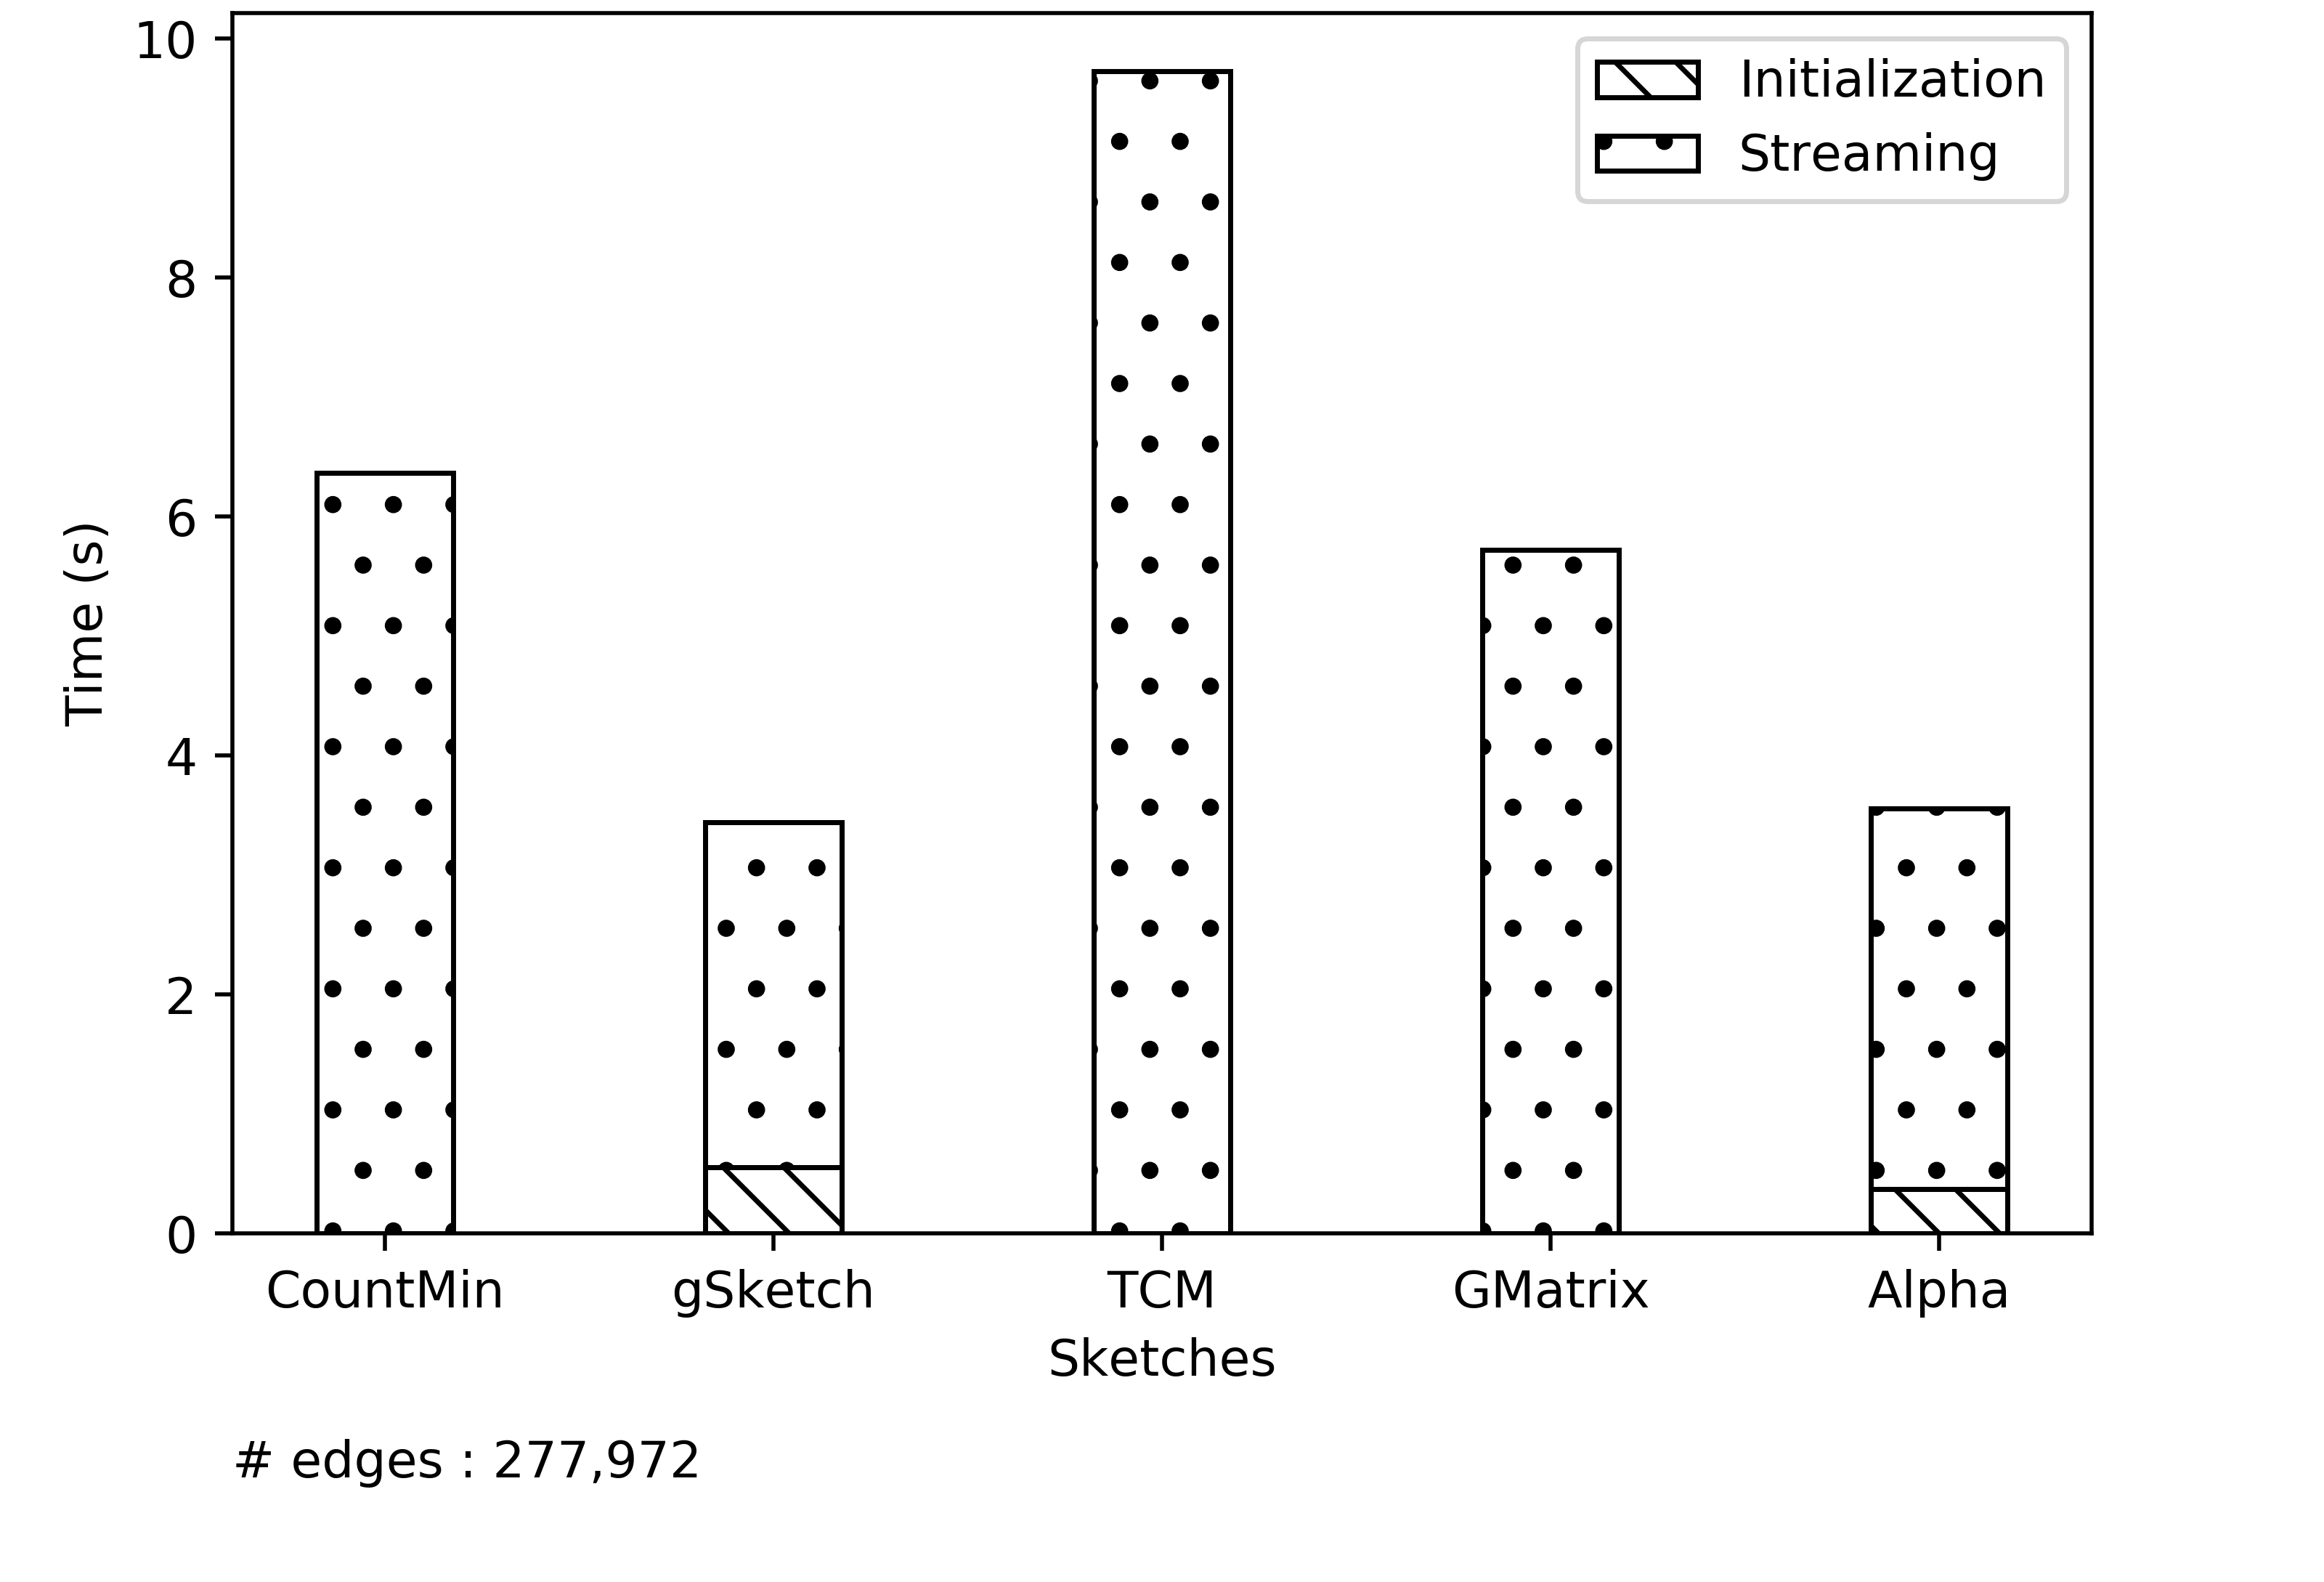
\includegraphics[width=0.85\textwidth]{results/buildtime/unicorn-wget-buildtime_1024}
    \vspace{-0.5cm}
    \caption{Build-time for unicorn-wget dataset}
    \label{fig:unicorn-wget-buildtime_1024}
\end{figure}

\begin{figure}[H]
    \centering 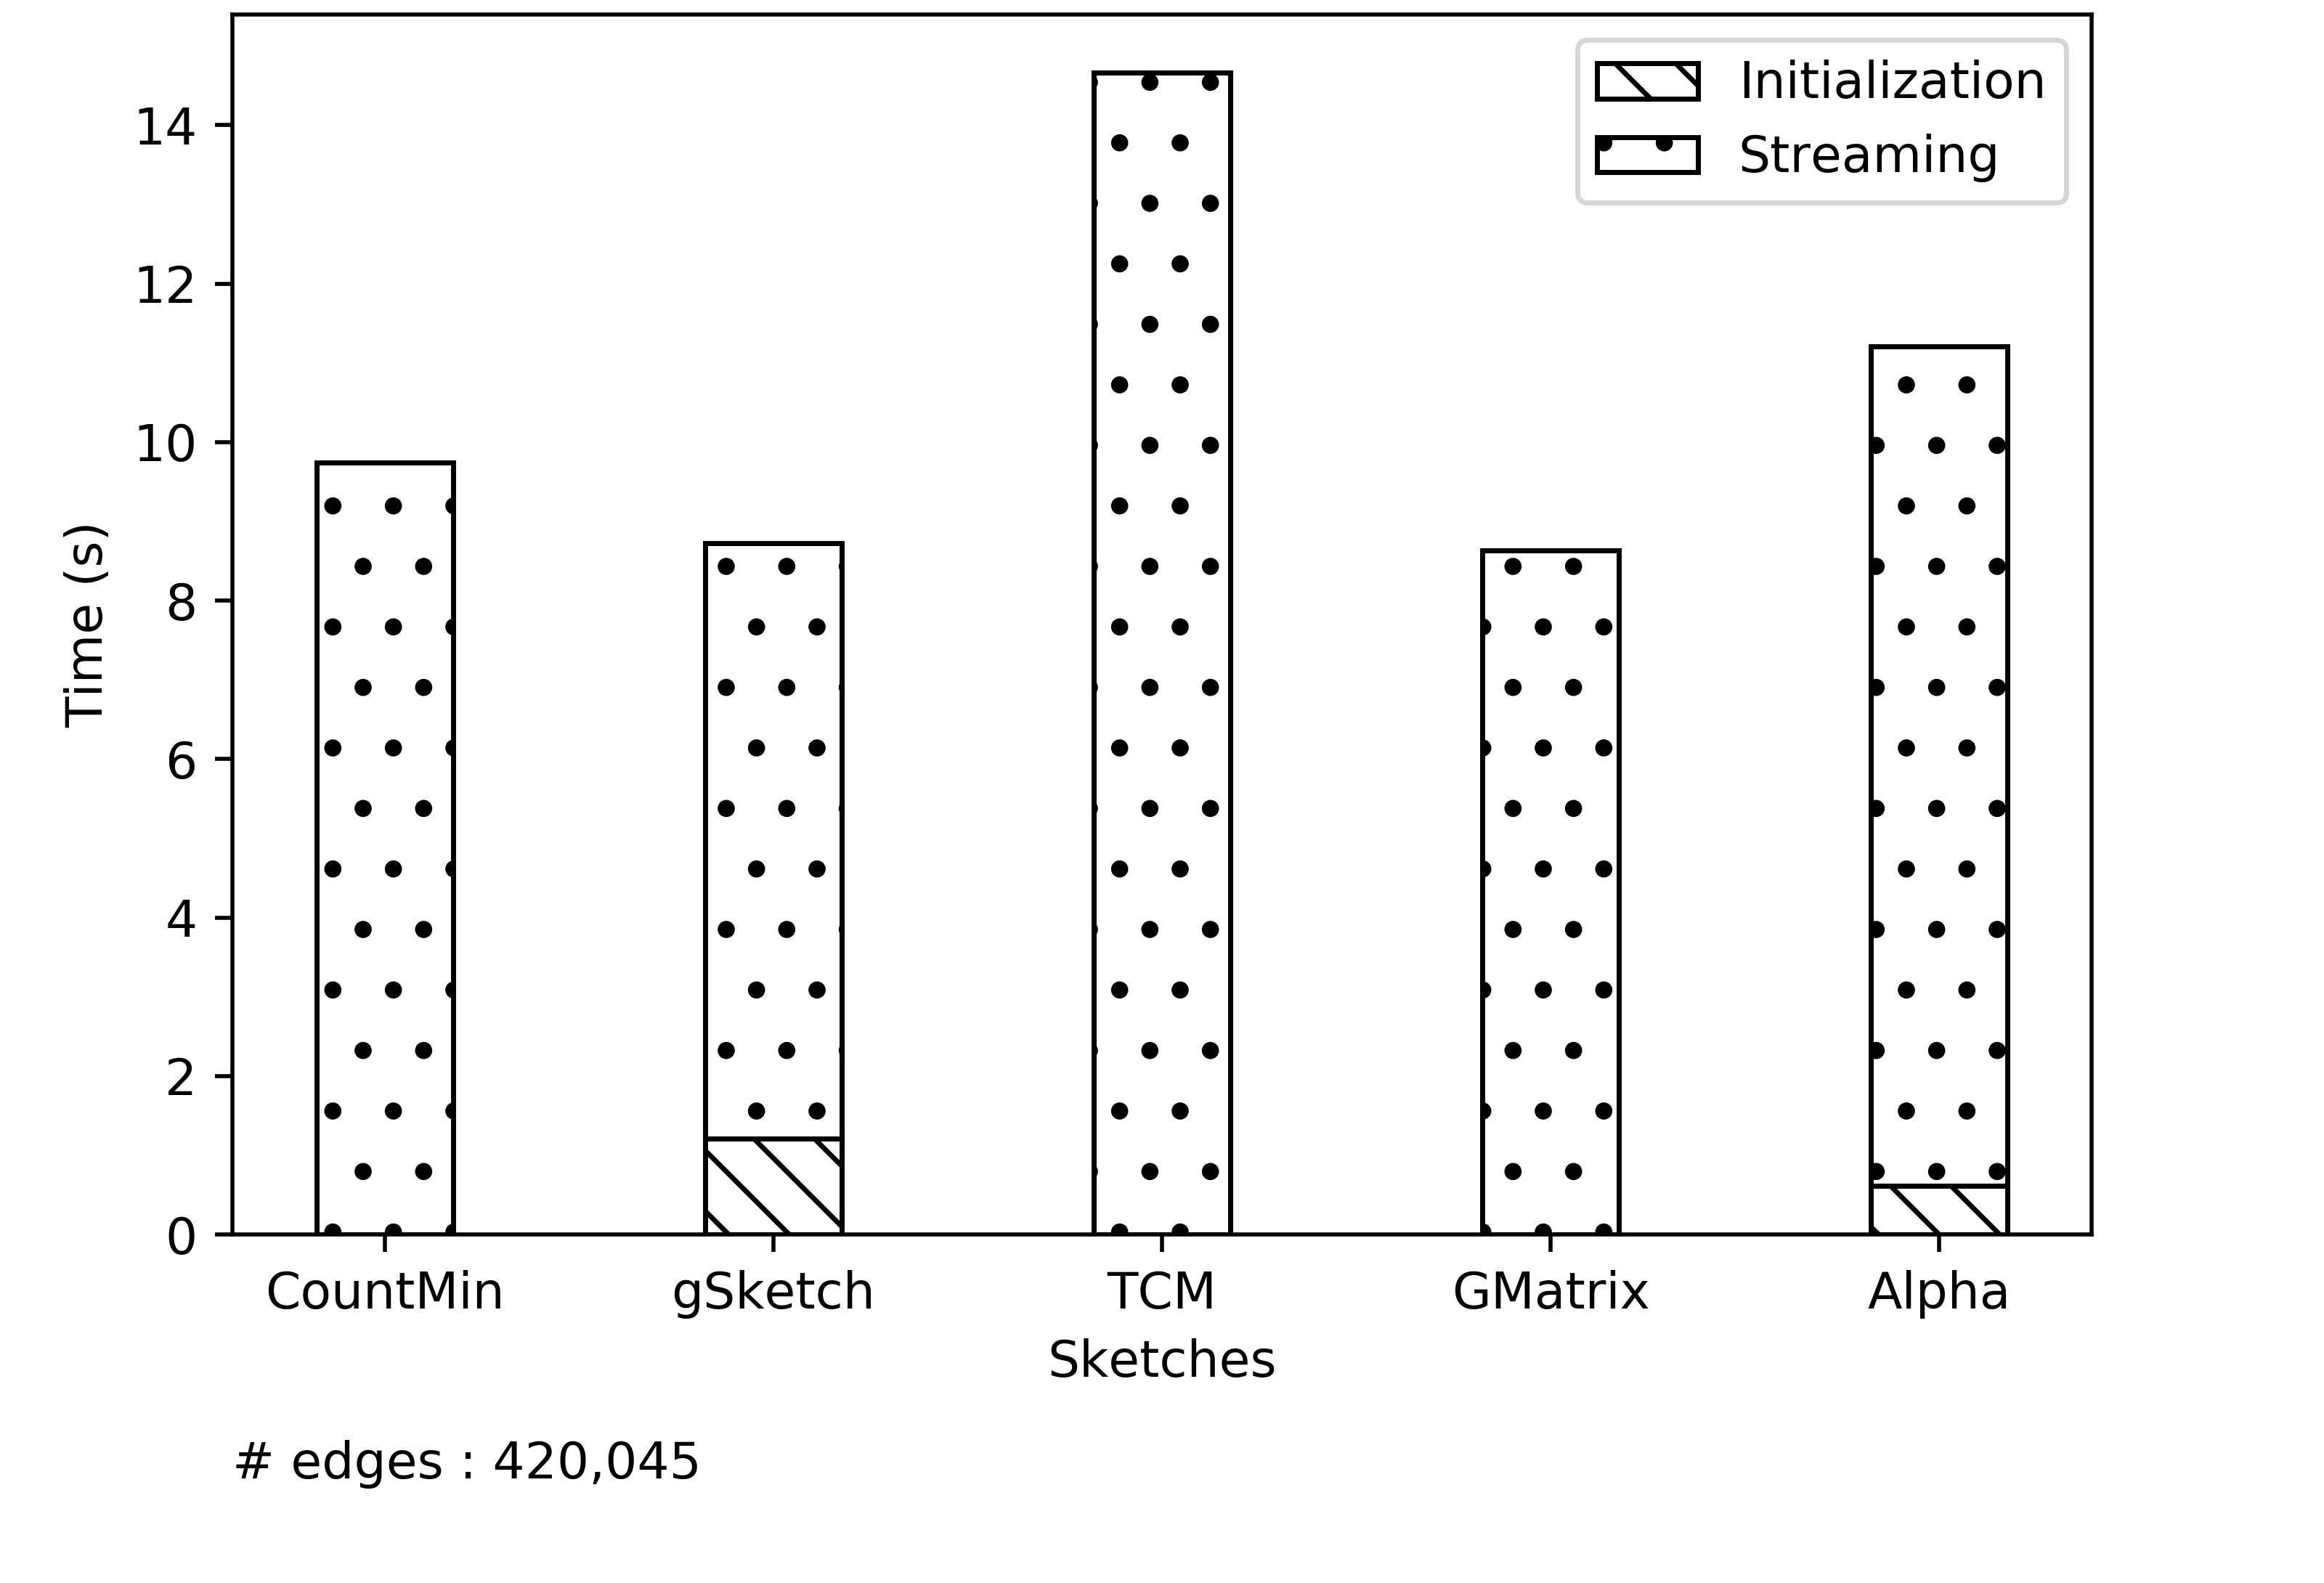
\includegraphics[width=0.85\textwidth]{results/buildtime/email-EuAll-buildtime_1024}
    \vspace{-0.5cm}
    \caption{Build-time for email-EuAll dataset}
    \label{fig:email-EuAll-buildtime_1024}
\end{figure}

\begin{figure}[H]
    \centering 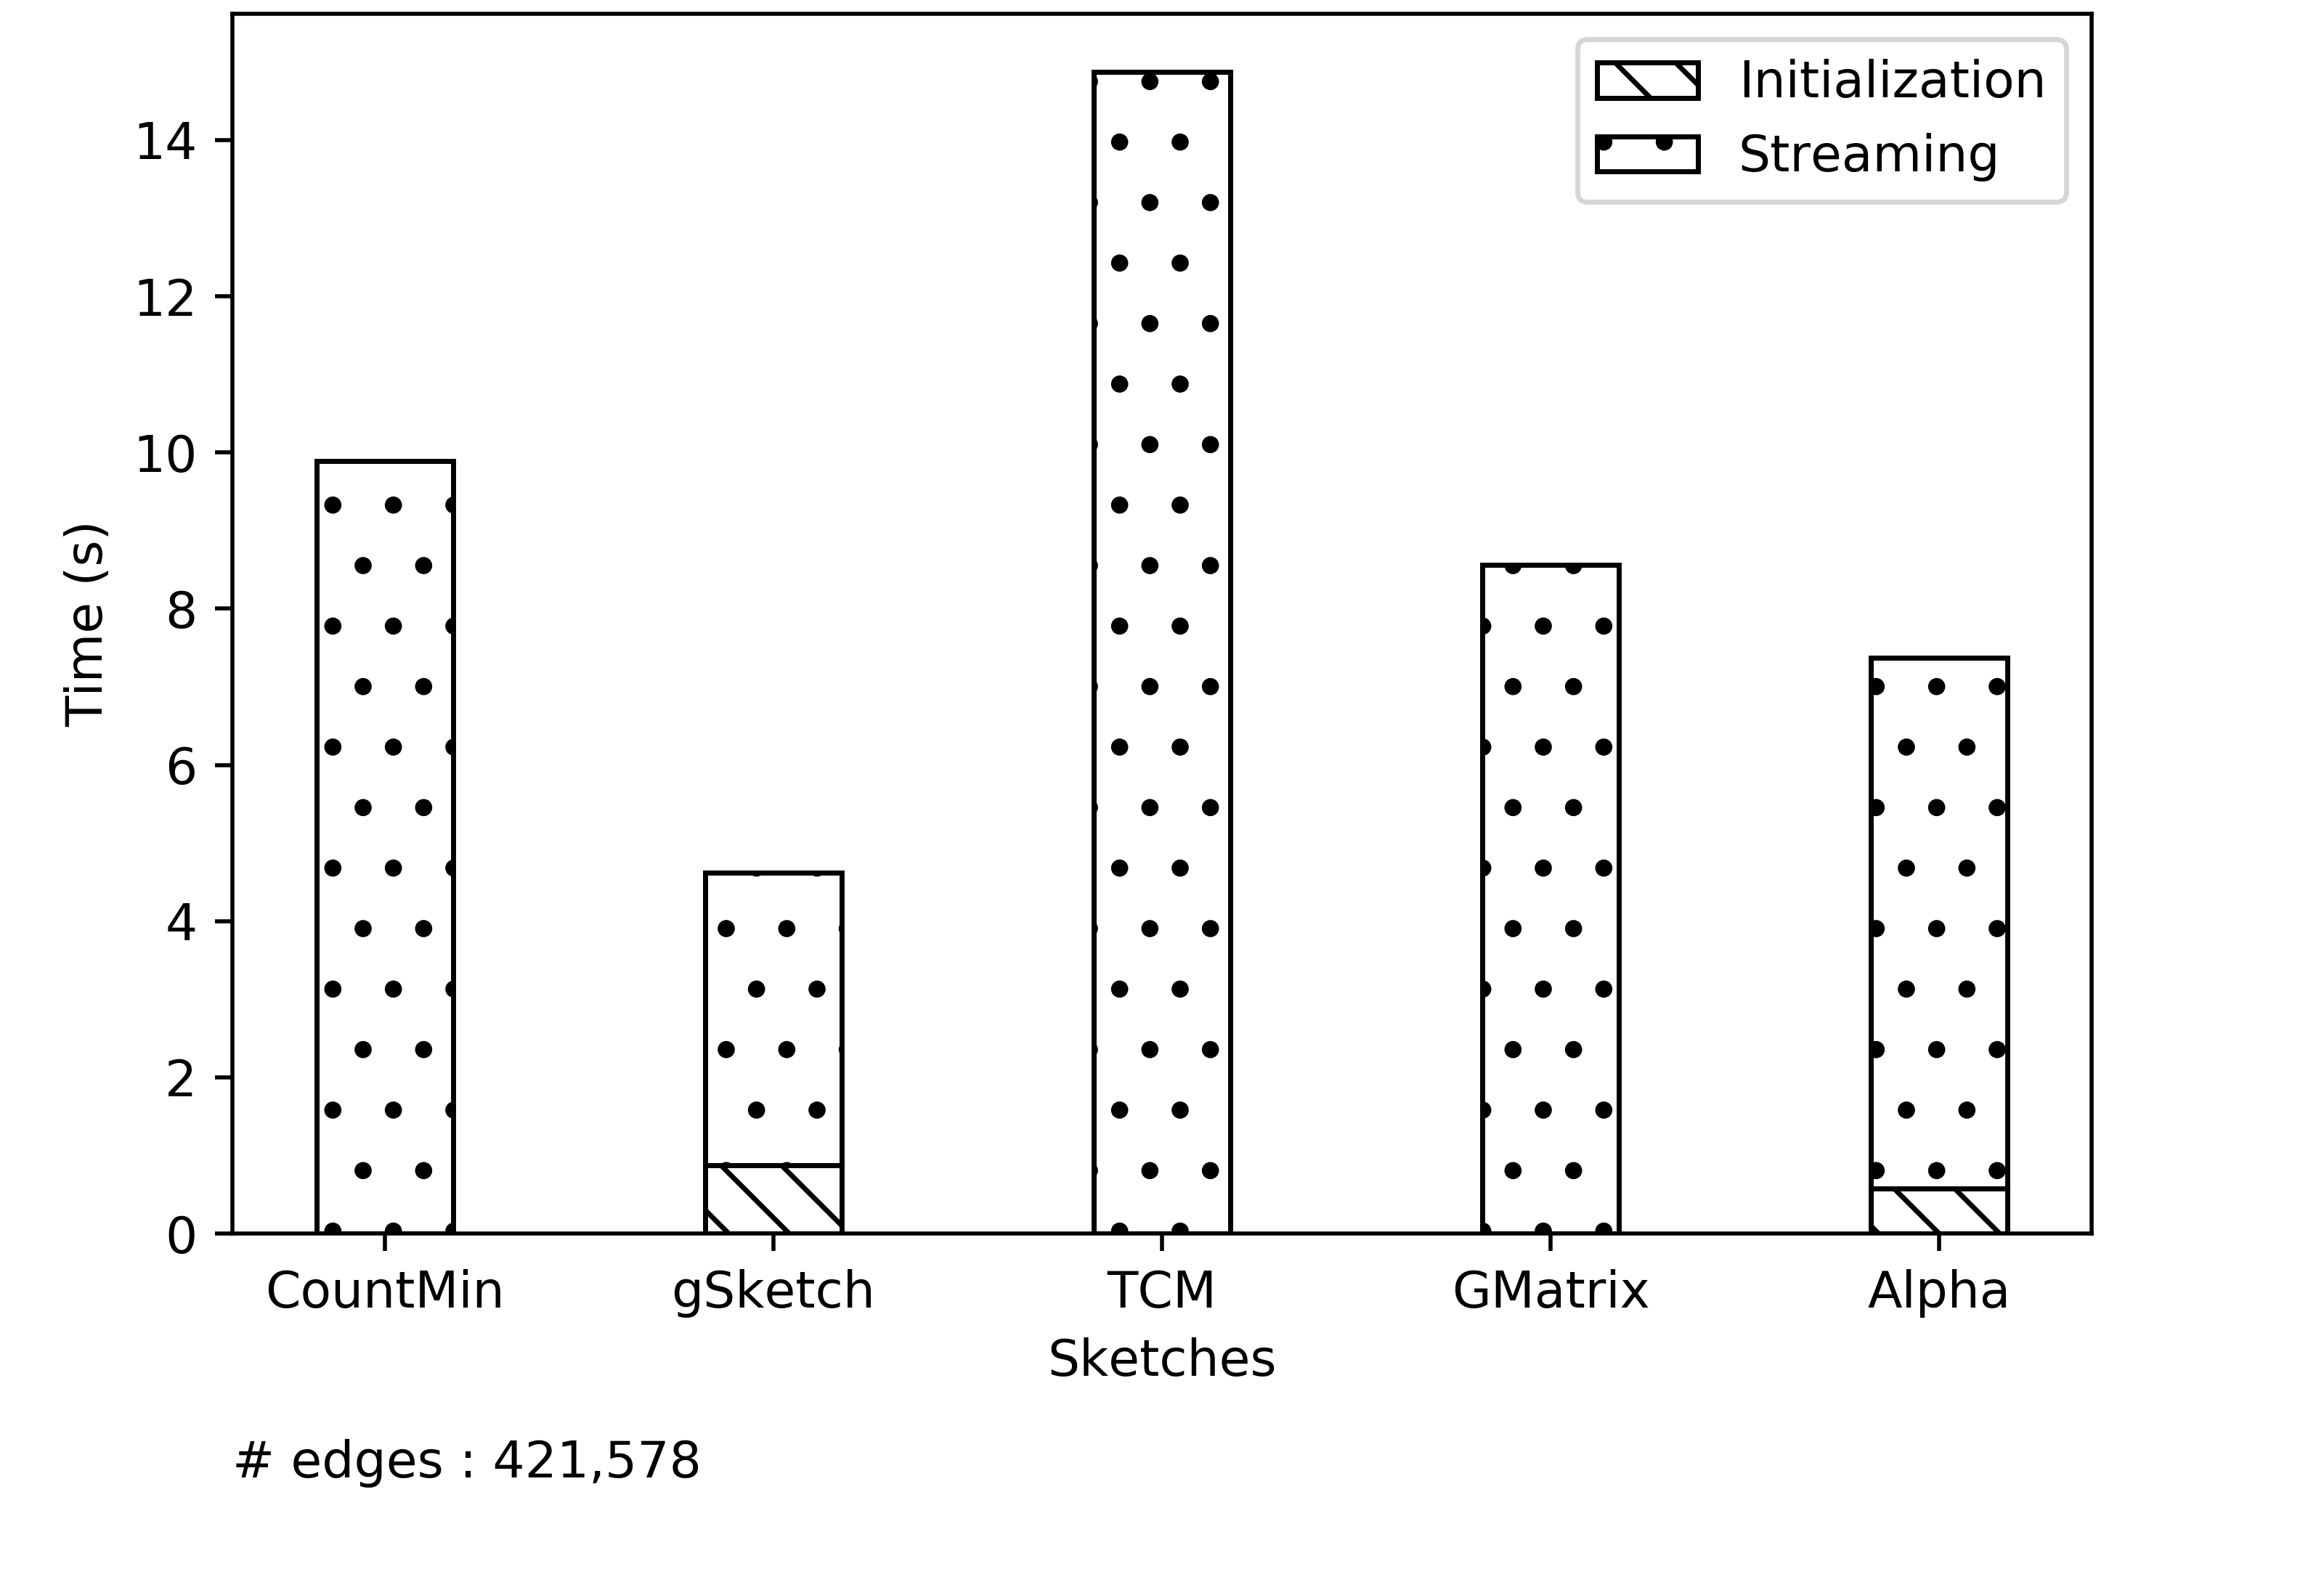
\includegraphics[width=0.85\textwidth]{results/buildtime/cit-HepPh-buildtime_1024}
    \vspace{-0.5cm}
    \caption{Build-time for cit-HepPh dataset}
    \label{fig:cit-HepPh-buildtime_1024}
\end{figure}

\begin{figure}[H]
    \centering 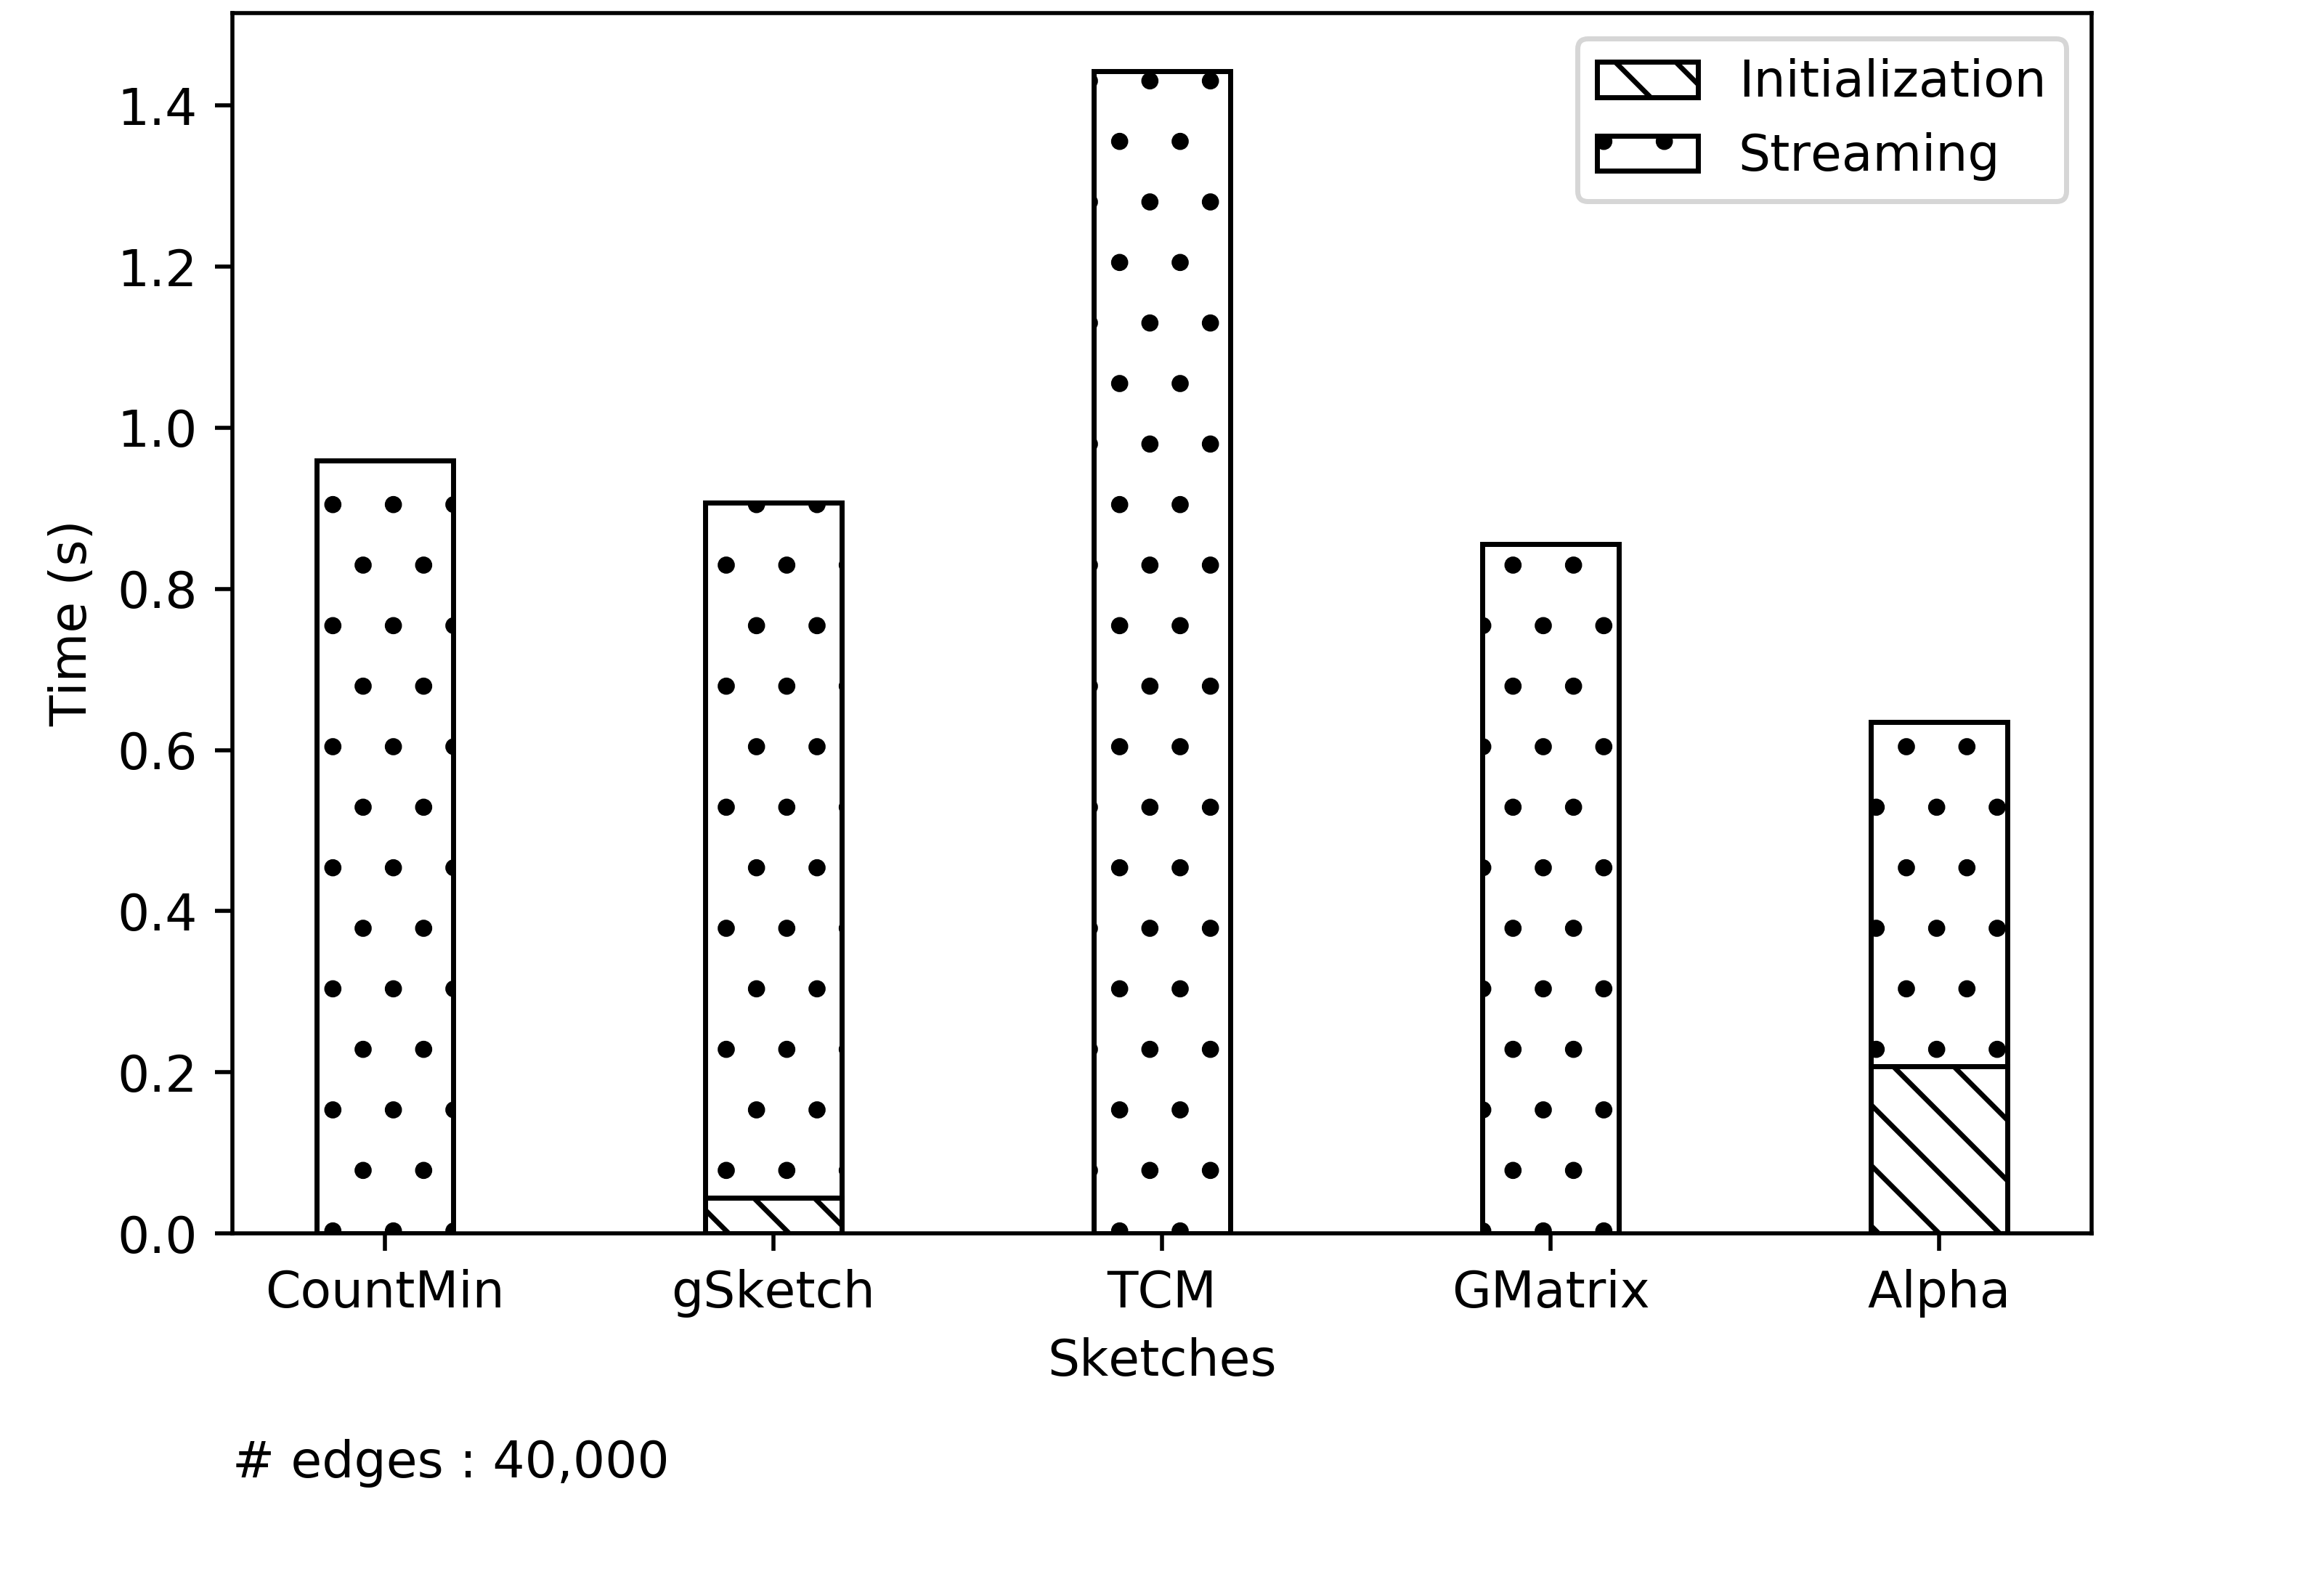
\includegraphics[width=0.85\textwidth]{results/buildtime/gen-scale-free-buildtime_1024}
    \vspace{-0.5cm}
    \caption{Build-time for gen-scale-free dataset}
    \label{fig:gen-scale-free-buildtime_1024}
\end{figure}

\begin{figure}[H]
    \centering 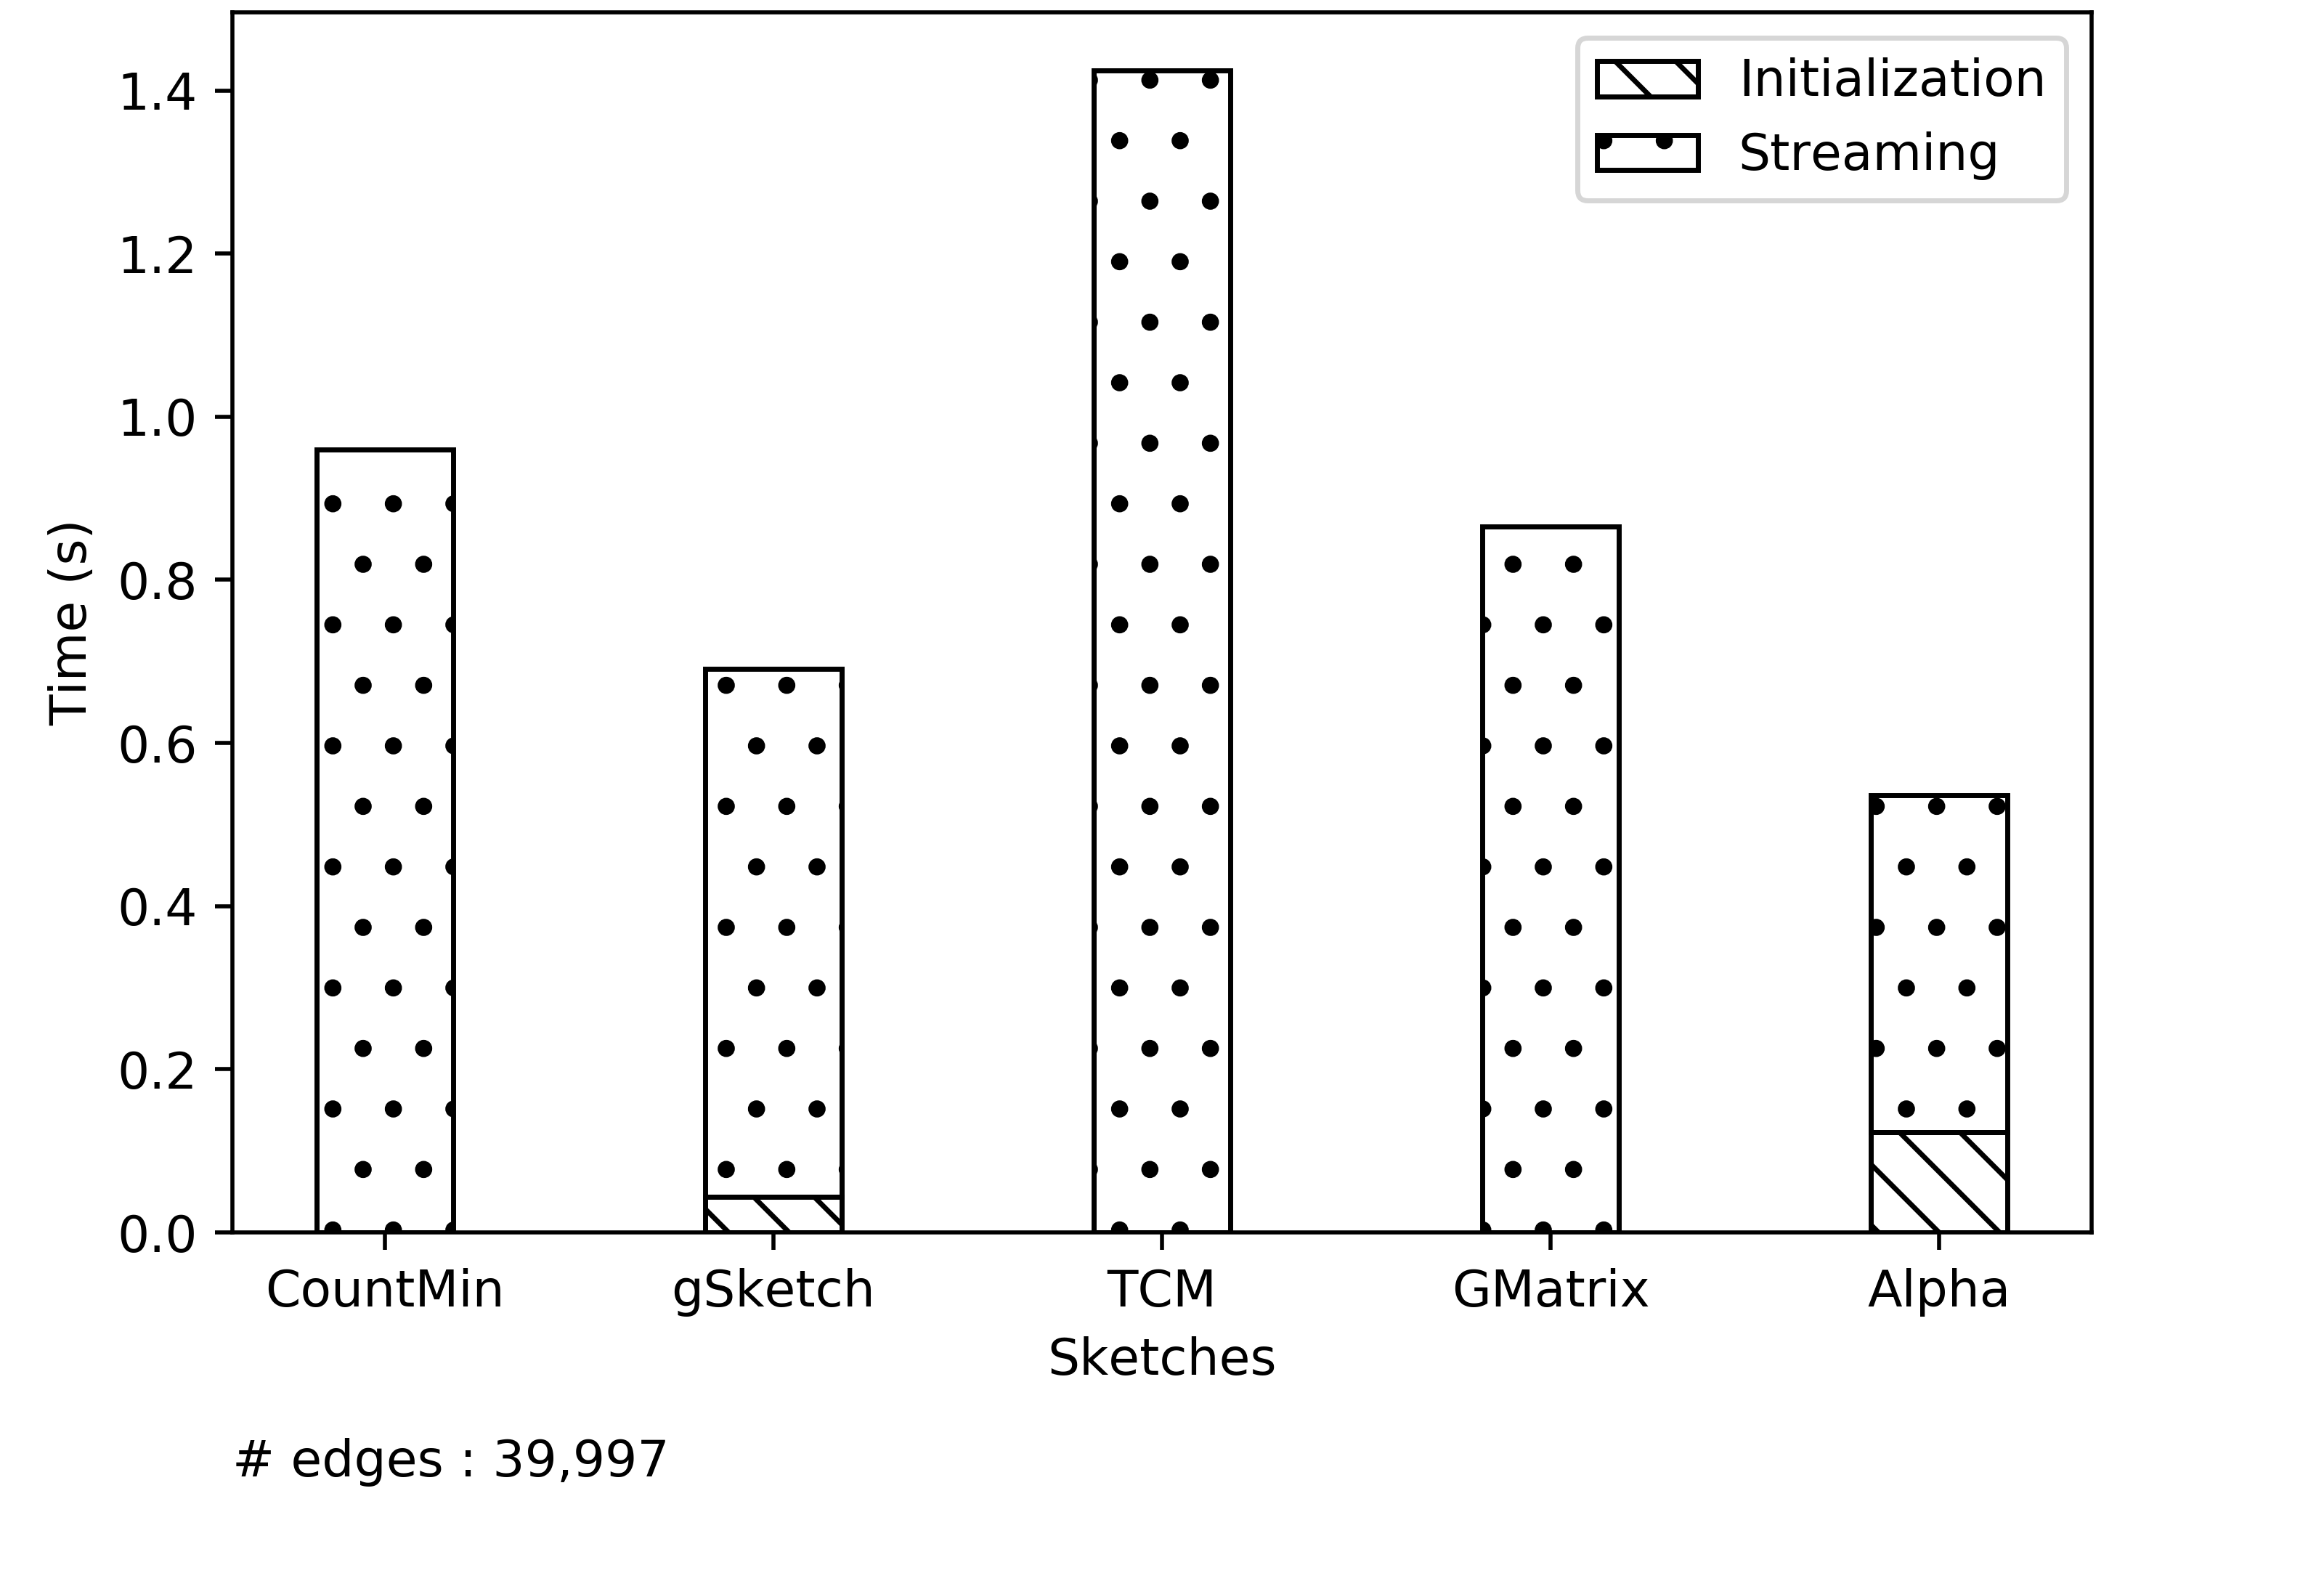
\includegraphics[width=0.85\textwidth]{results/buildtime/gen-small-world-buildtime_1024}
    \vspace{-0.5cm}
    \caption{Build-time for gen-small-world dataset}
    \label{fig:gen-small-world-buildtime_1024}
\end{figure}

\subsection*{Observations and inferences}

\paragraph{}
Both the gSketch and Alpha has been initialized with a sample of 10,000 edges from the original stream. Thus the gSketch and Alpha have comparable initialization times. The other sketches do not have an initialization time cost as they don't possess initialization stages. All the sketches were created with 1 MB memory allocation.

\paragraph{}
In the results for the datasets, unicorn-wget in \autoref{fig:unicorn-wget-buildtime_1024}, cit-HepPh in \autoref{fig:cit-HepPh-buildtime_1024}, gen-scale-free in \autoref{fig:gen-scale-free-buildtime_1024} and gen-small-world in \autoref{fig:gen-small-world-buildtime_1024}; Alpha has taken a significantly lower time for the streaming than all the other sketches except for gSketch.

\paragraph{}
Sketch creation and the streaming time of Alpha is significantly better than the CountMin, TCM and GMatrix for 4/5 datasets that were tested. Only gSketch has performed slightly better than Alpha in this regard. However this can be dismissed as gSketch is a only a frequency approximation sketch. Therefor we are able to conclude that Alpha is generally faster than the existing sketching techniques in creation of the summarized sketch.
\section{Average Relative Error}
\label{section:results_are}

\subsection*{Purpose}

\paragraph{}
To compare the average relative error of each sketch under different types of graph streams.

\paragraph{}
Average relative error has been previously defined in \autoref{section:metrics_are}. For this section of testing, the average relative error of simple edge frequency queries has been measured.

\subsection*{Results}

\begin{figure}[H]
    \centering 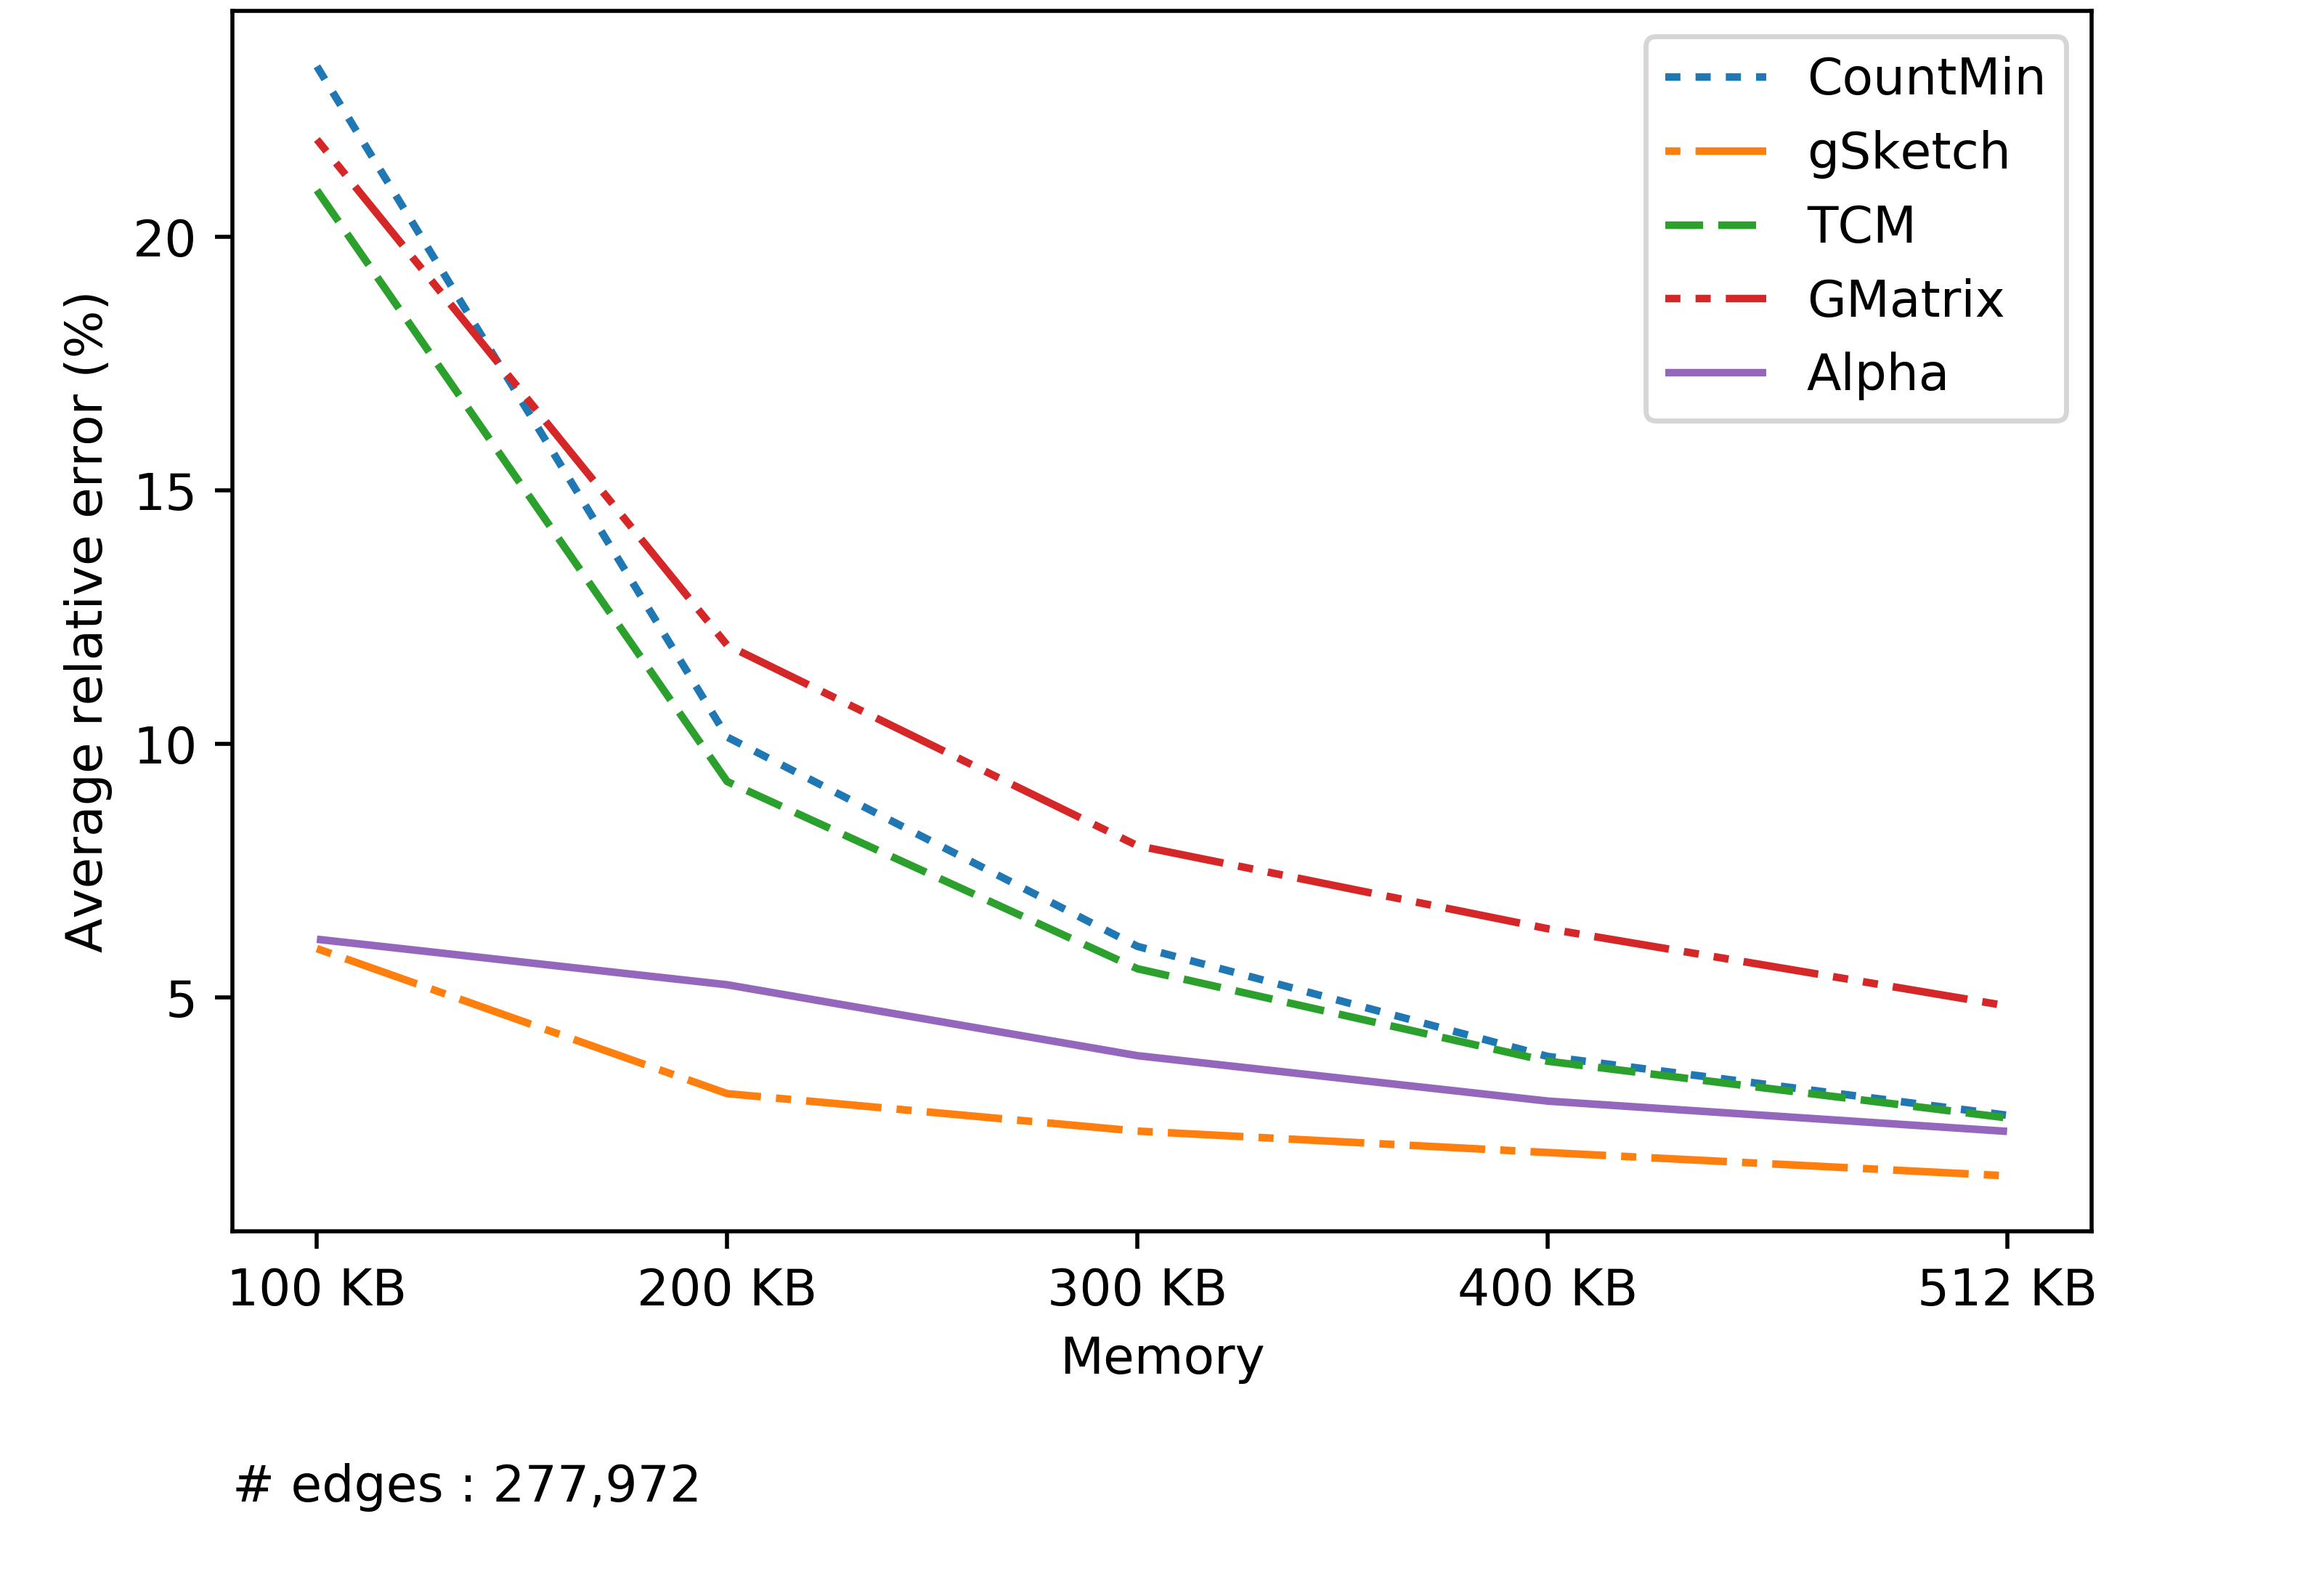
\includegraphics[width=0.85\textwidth]{results/are/unicorn-wget-are}
    \vspace{-0.5cm}
    \caption{Average relative error vs Memory for unicorn-wget dataset}
    \label{fig:unicorn-wget-are}
\end{figure}

\begin{figure}[H]
    \centering 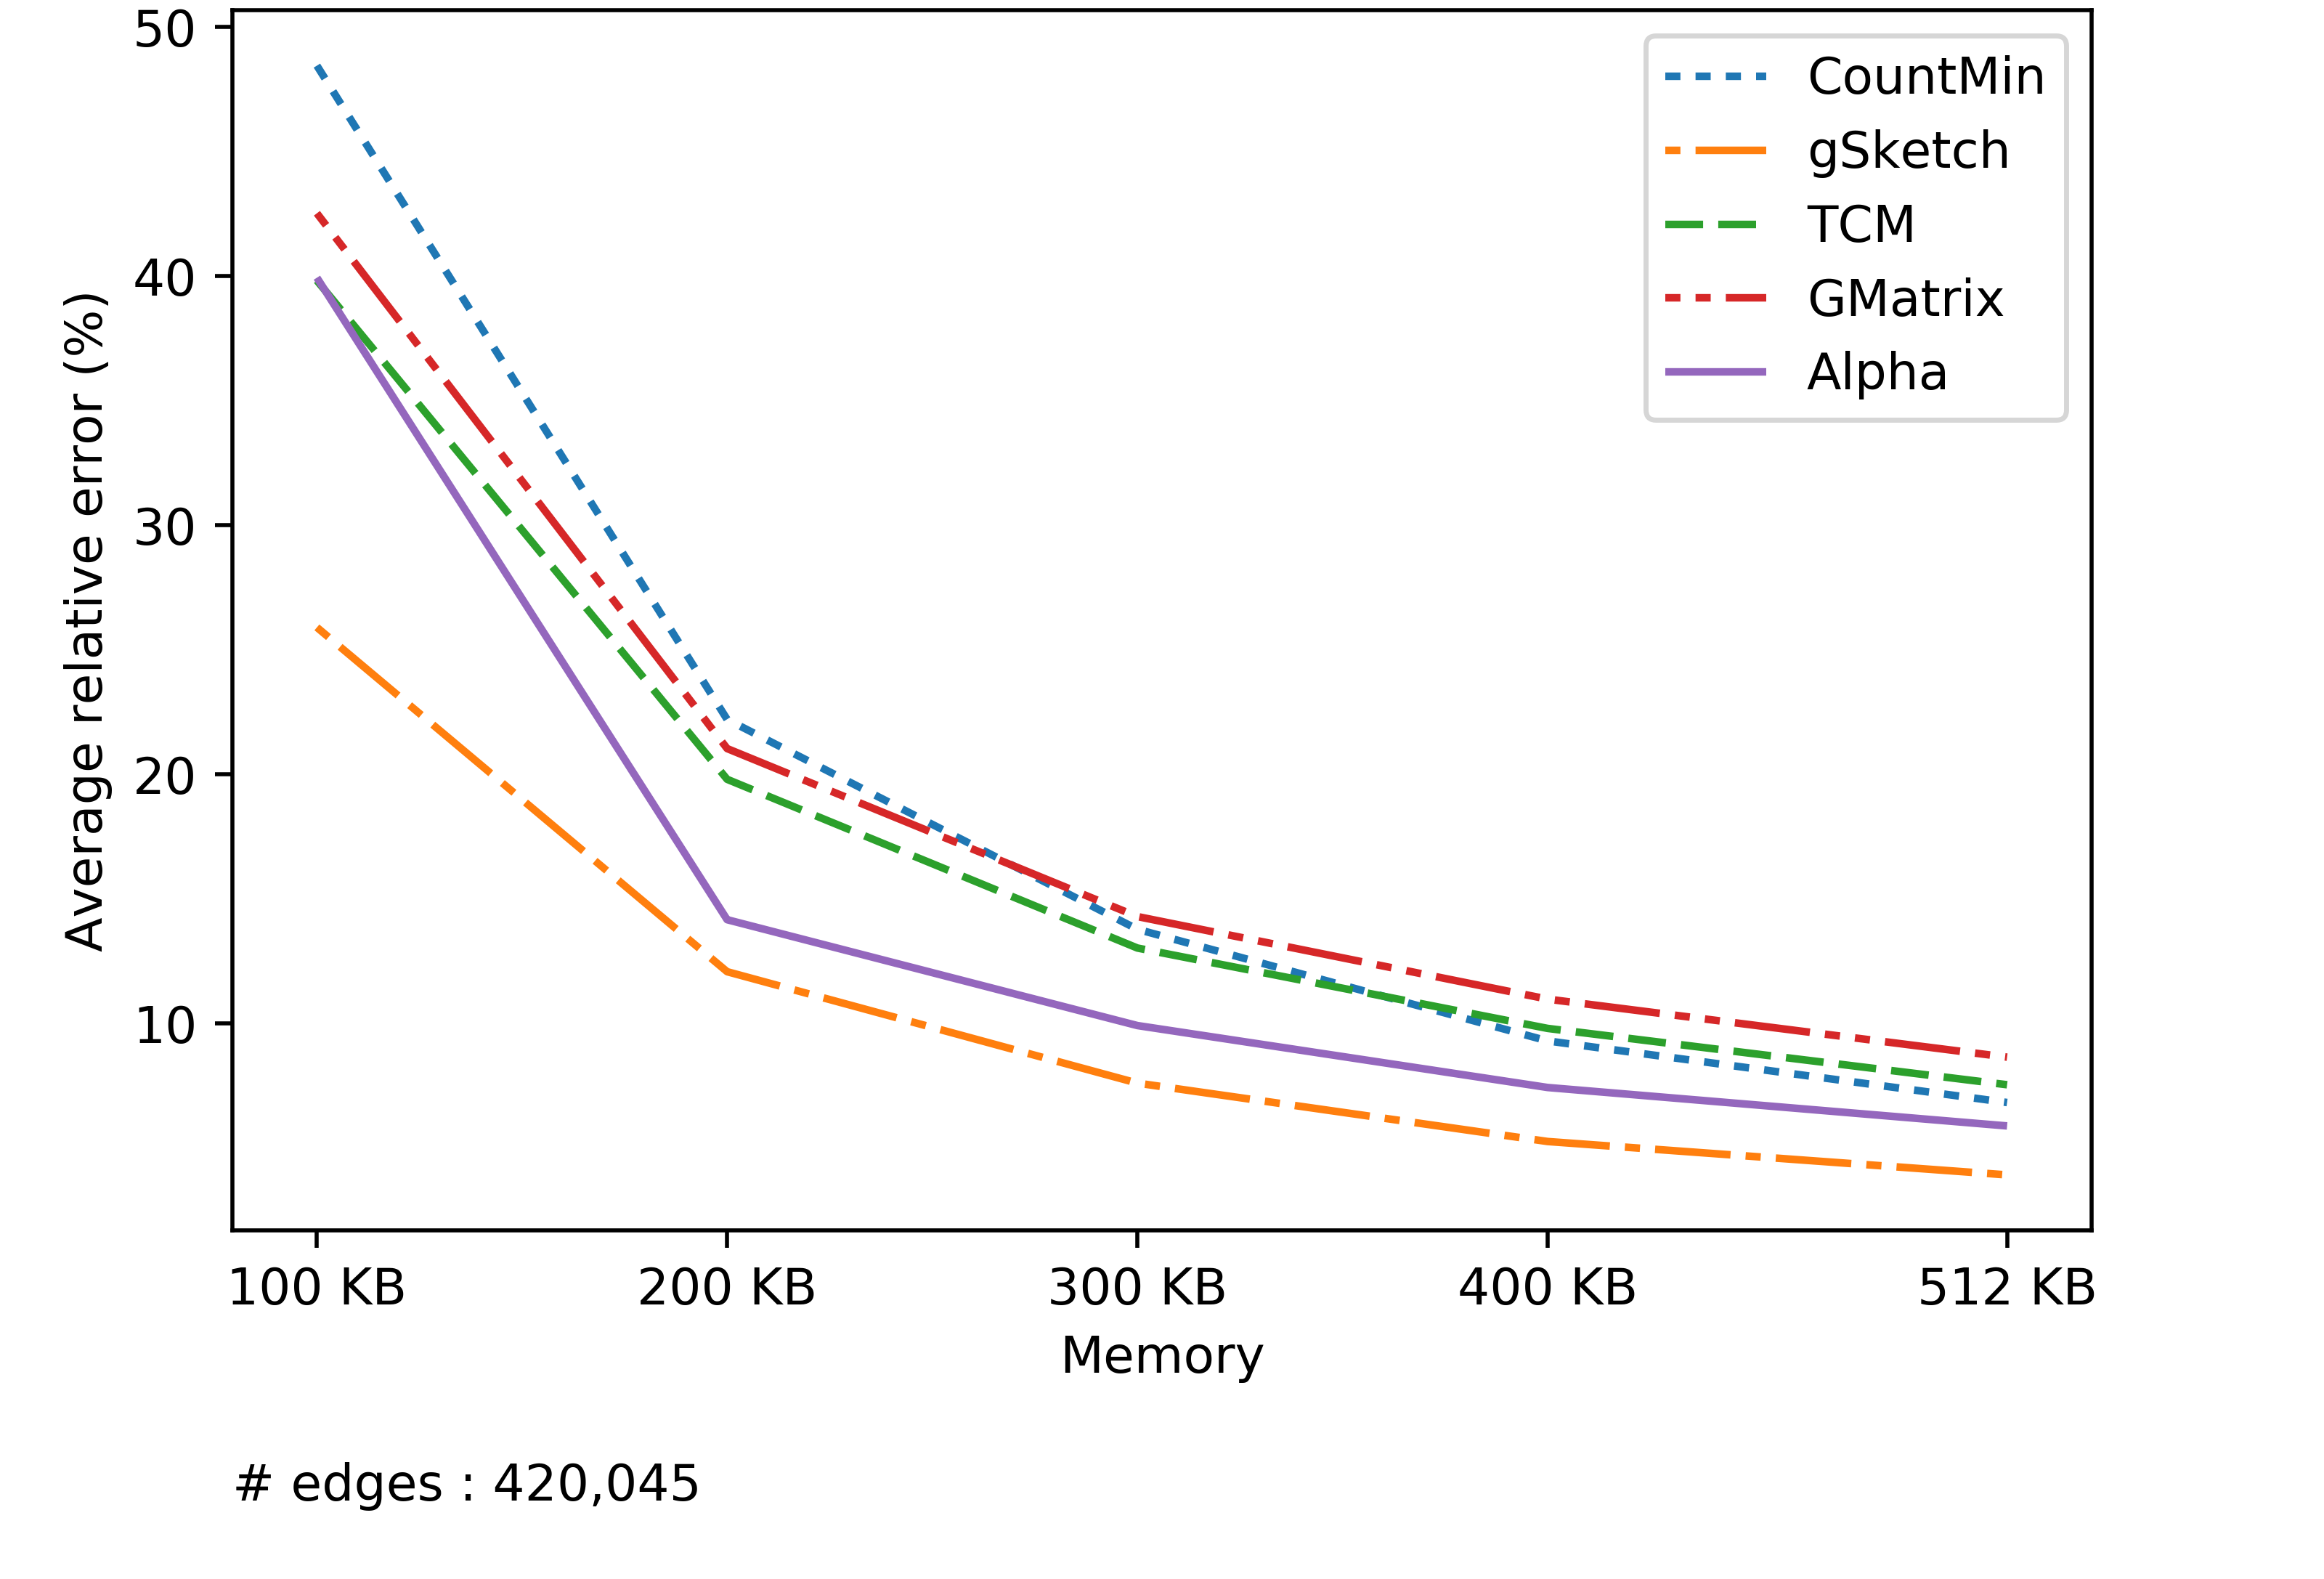
\includegraphics[width=0.85\textwidth]{results/are/email-EuAll-are}
    \vspace{-0.5cm}
    \caption{Average relative error vs Memory for email-EuAll dataset}
    \label{fig:email-EuAll-are}
\end{figure}

\begin{figure}[H]
    \centering 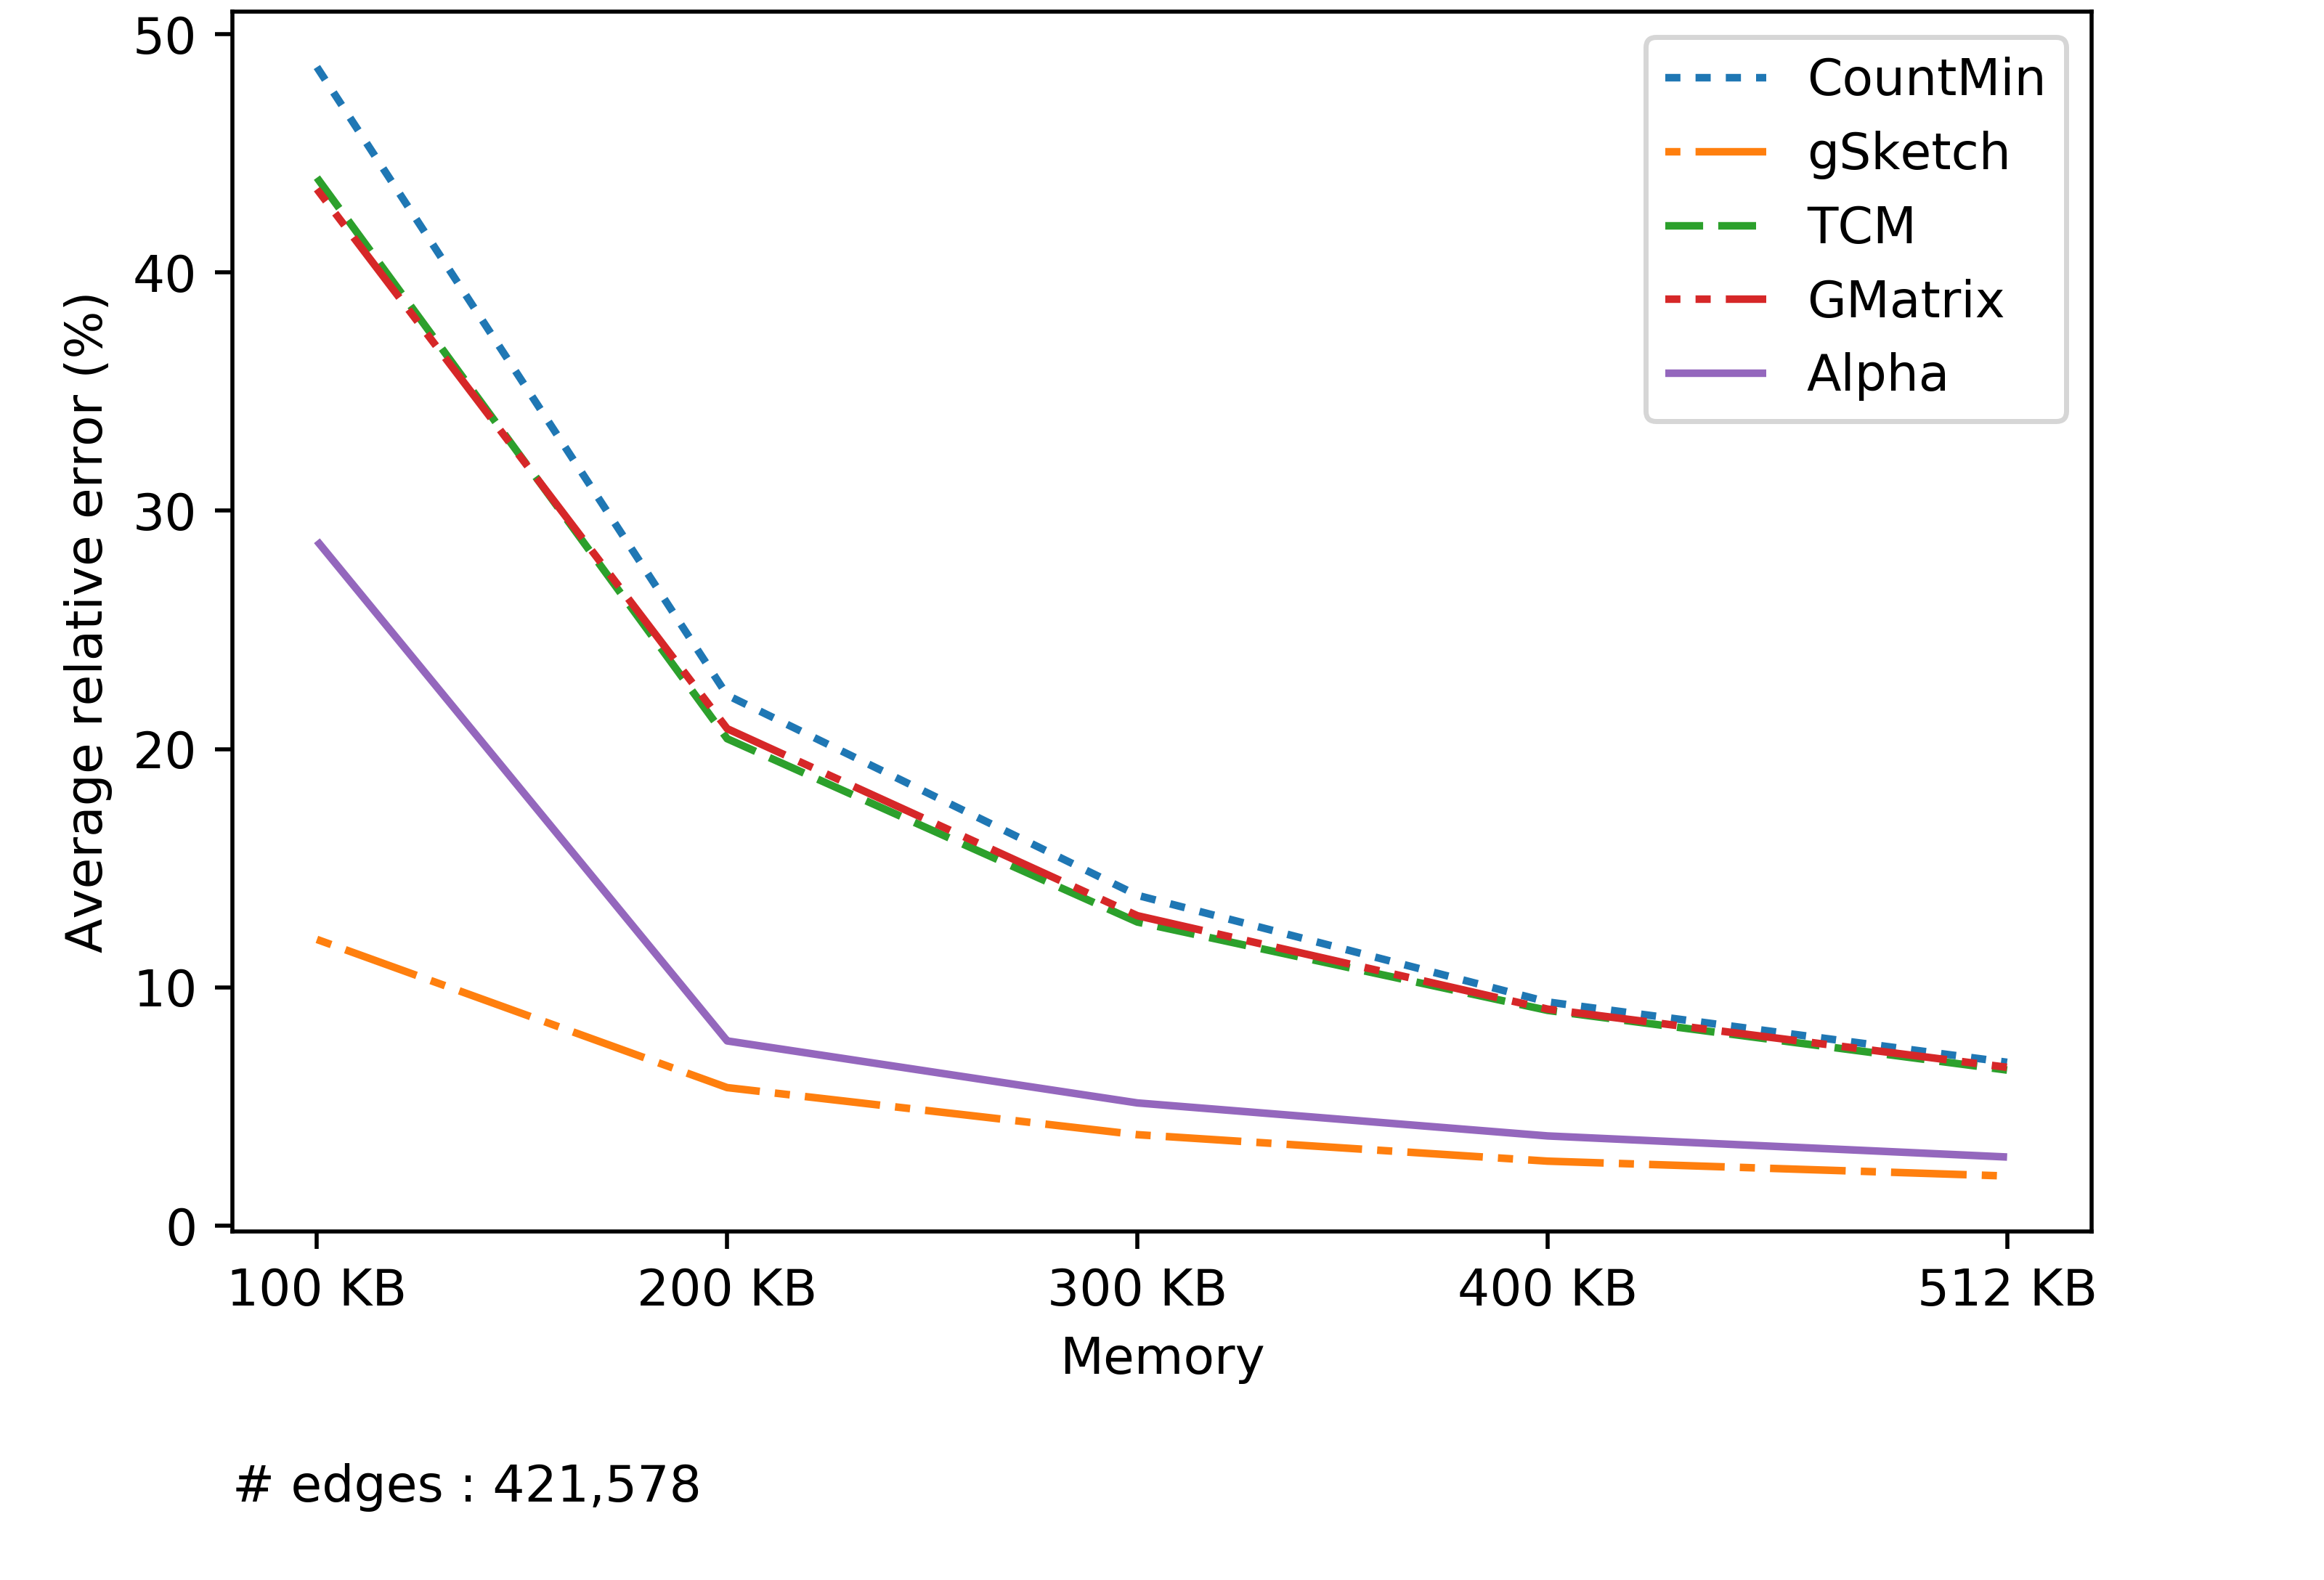
\includegraphics[width=0.85\textwidth]{results/are/cit-HepPh-are}
    \vspace{-0.5cm}
    \caption{Average relative error vs Memory for cit-HepPh dataset}
    \label{fig:cit-HepPh-are}
\end{figure}

\begin{figure}[H]
    \centering 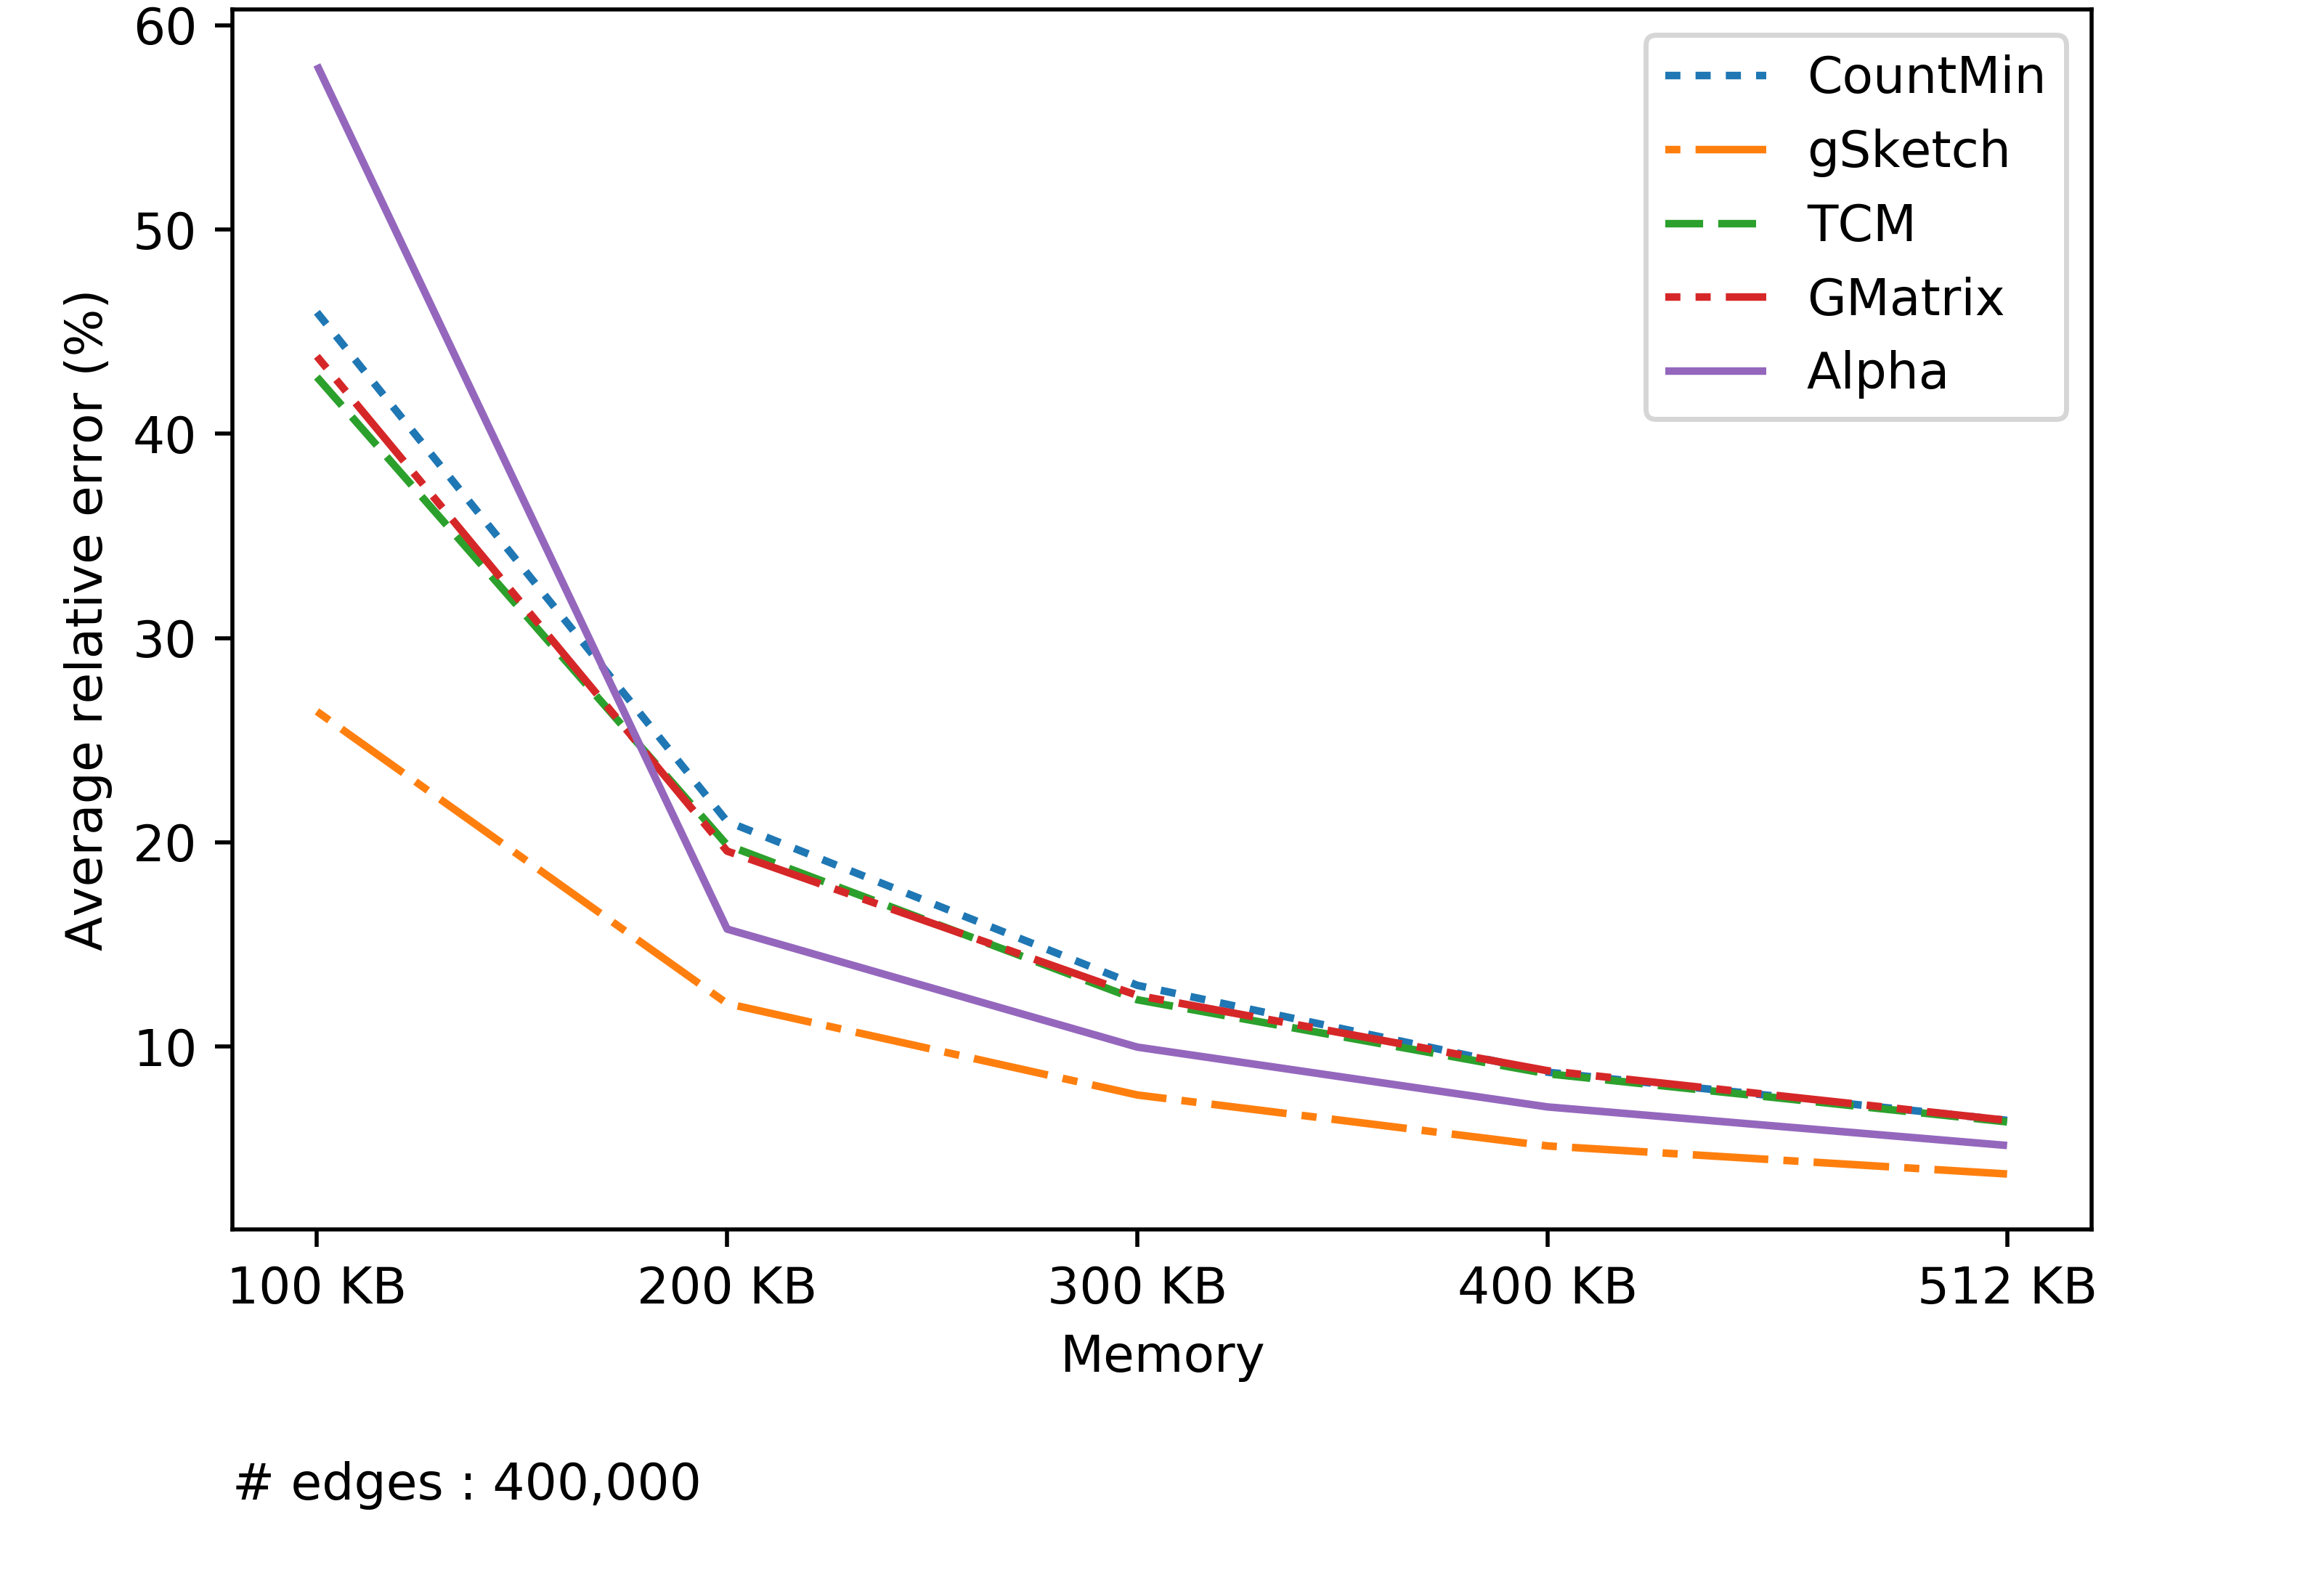
\includegraphics[width=0.85\textwidth]{results/are/gen-scale-free-are}
    \vspace{-0.5cm}
    \caption{Average relative error vs Memory for gen-scale-free dataset}
    \label{fig:gen-scale-free-are}
\end{figure}

\begin{figure}[H]
    \centering 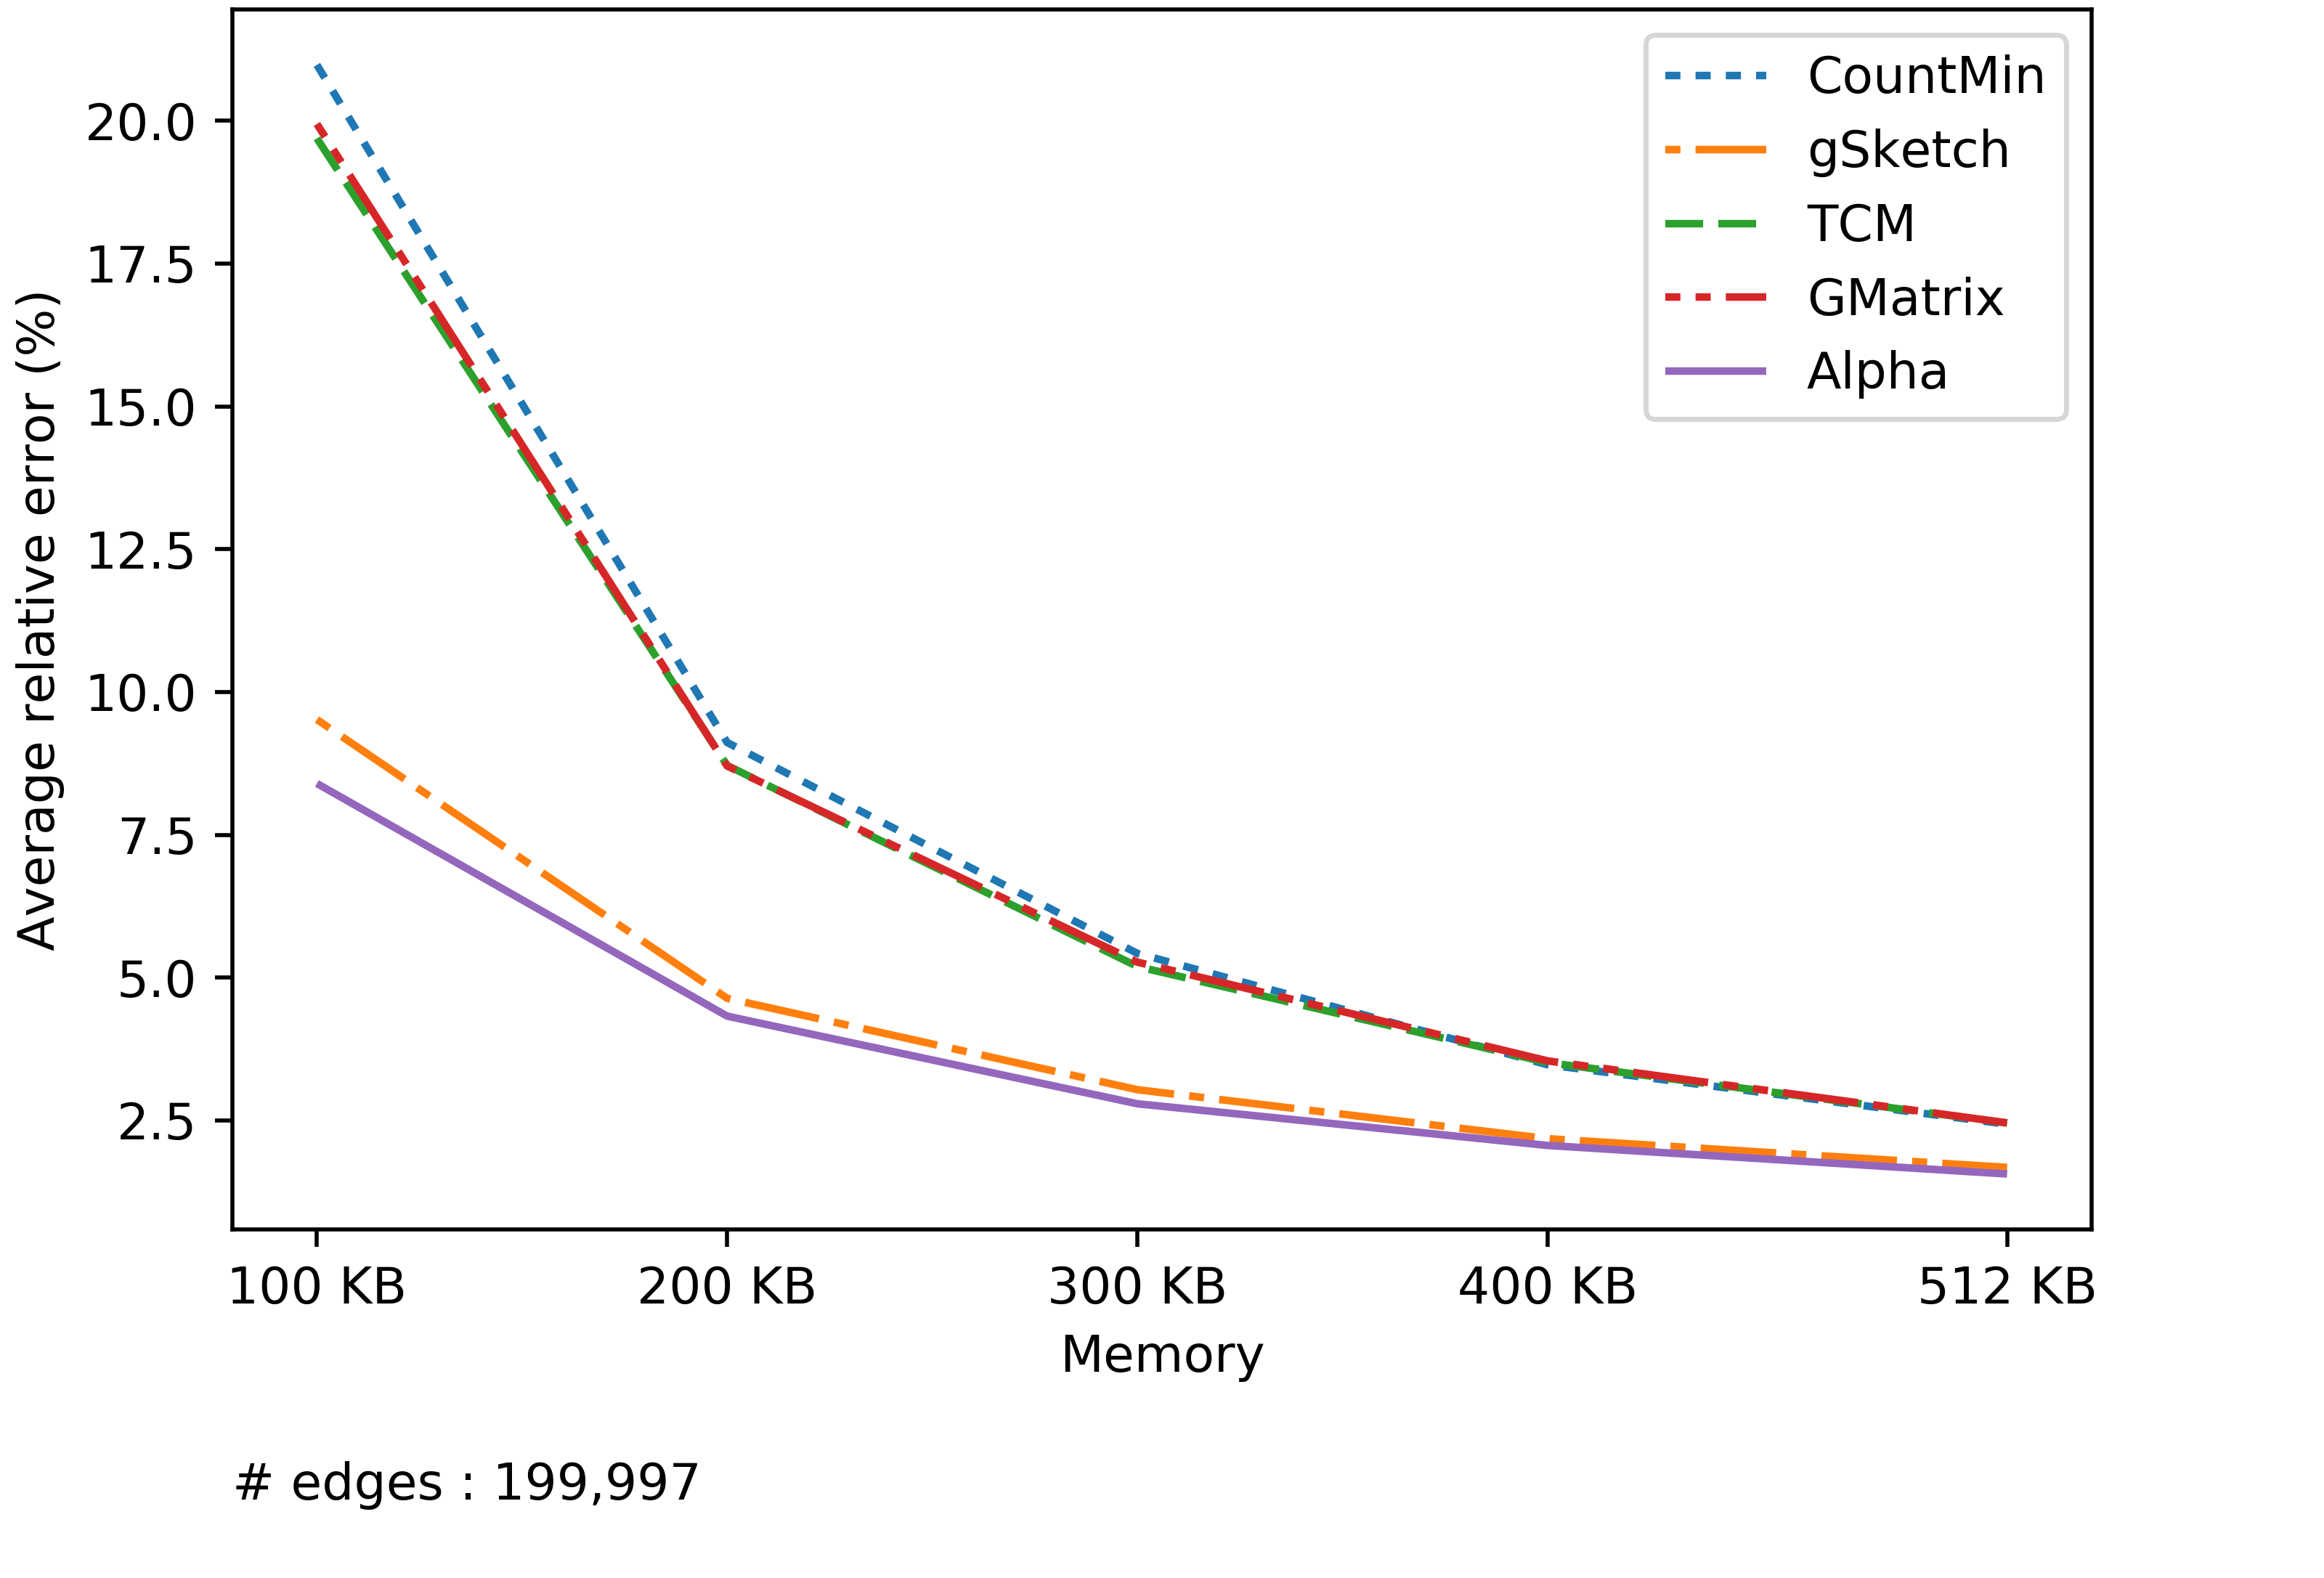
\includegraphics[width=0.85\textwidth]{results/are/gen-small-world-are}
    \vspace{-0.5cm}
    \caption{Average relative error vs Memory for gen-small-world dataset}
    \label{fig:gen-small-world-are}
\end{figure}

\subsection*{Observations and inferences}

\paragraph{}
In the results for the datasets, unicorn-wget in \autoref{fig:unicorn-wget-are}, email-EuAll in \autoref{fig:email-EuAll-are}, cit-HepPh in \autoref{fig:cit-HepPh-are}, gen-scale-free in \autoref{fig:gen-scale-free-are} and gen-small-world in \autoref{fig:gen-small-world-are}; Alpha has a significantly lower average relative error in general than all the other sketches except for gSketch.

\paragraph{}
In the \autoref{fig:gen-scale-free-are}, for 100 KB sketch size, Alpha has a higher average relative error than all the other sketches. This could possibly be a result of over-partitioning a smaller sketch such that the final error of the queries are worse than the unpartitioned sketch.

\paragraph{}
Alpha has the lowest average relative error for the gen-small-world dataset depicted in \autoref{fig:gen-small-world-are}. Thus it is evidant that Alpha is able to surpass the accuracy levels of gSketch in some cases.

\paragraph{}
Alpha has a much lower average relative error than TCM and GMatrix for all the tested datasets, proving its superiority over the existing sketching algorithms. It has even surpassed approximate frequency sketches like CountMin in this regard.
\section{Number of Effective Queries}

\subsection*{Purpose}

\paragraph{}
To compare the number of effective queries of each sketch under different types of graph streams. 

\paragraph{}
Number of effective queries has been previously defined in the \autoref{section:metrics_neq}. For this experiment, a simple edge query has been selected as the type of the query. If the value of the edge query in the sketch matched the value of the edge query in the original graph, it was considered as an effective query.

\subsection*{Results}

\begin{figure}[H]
    \centering 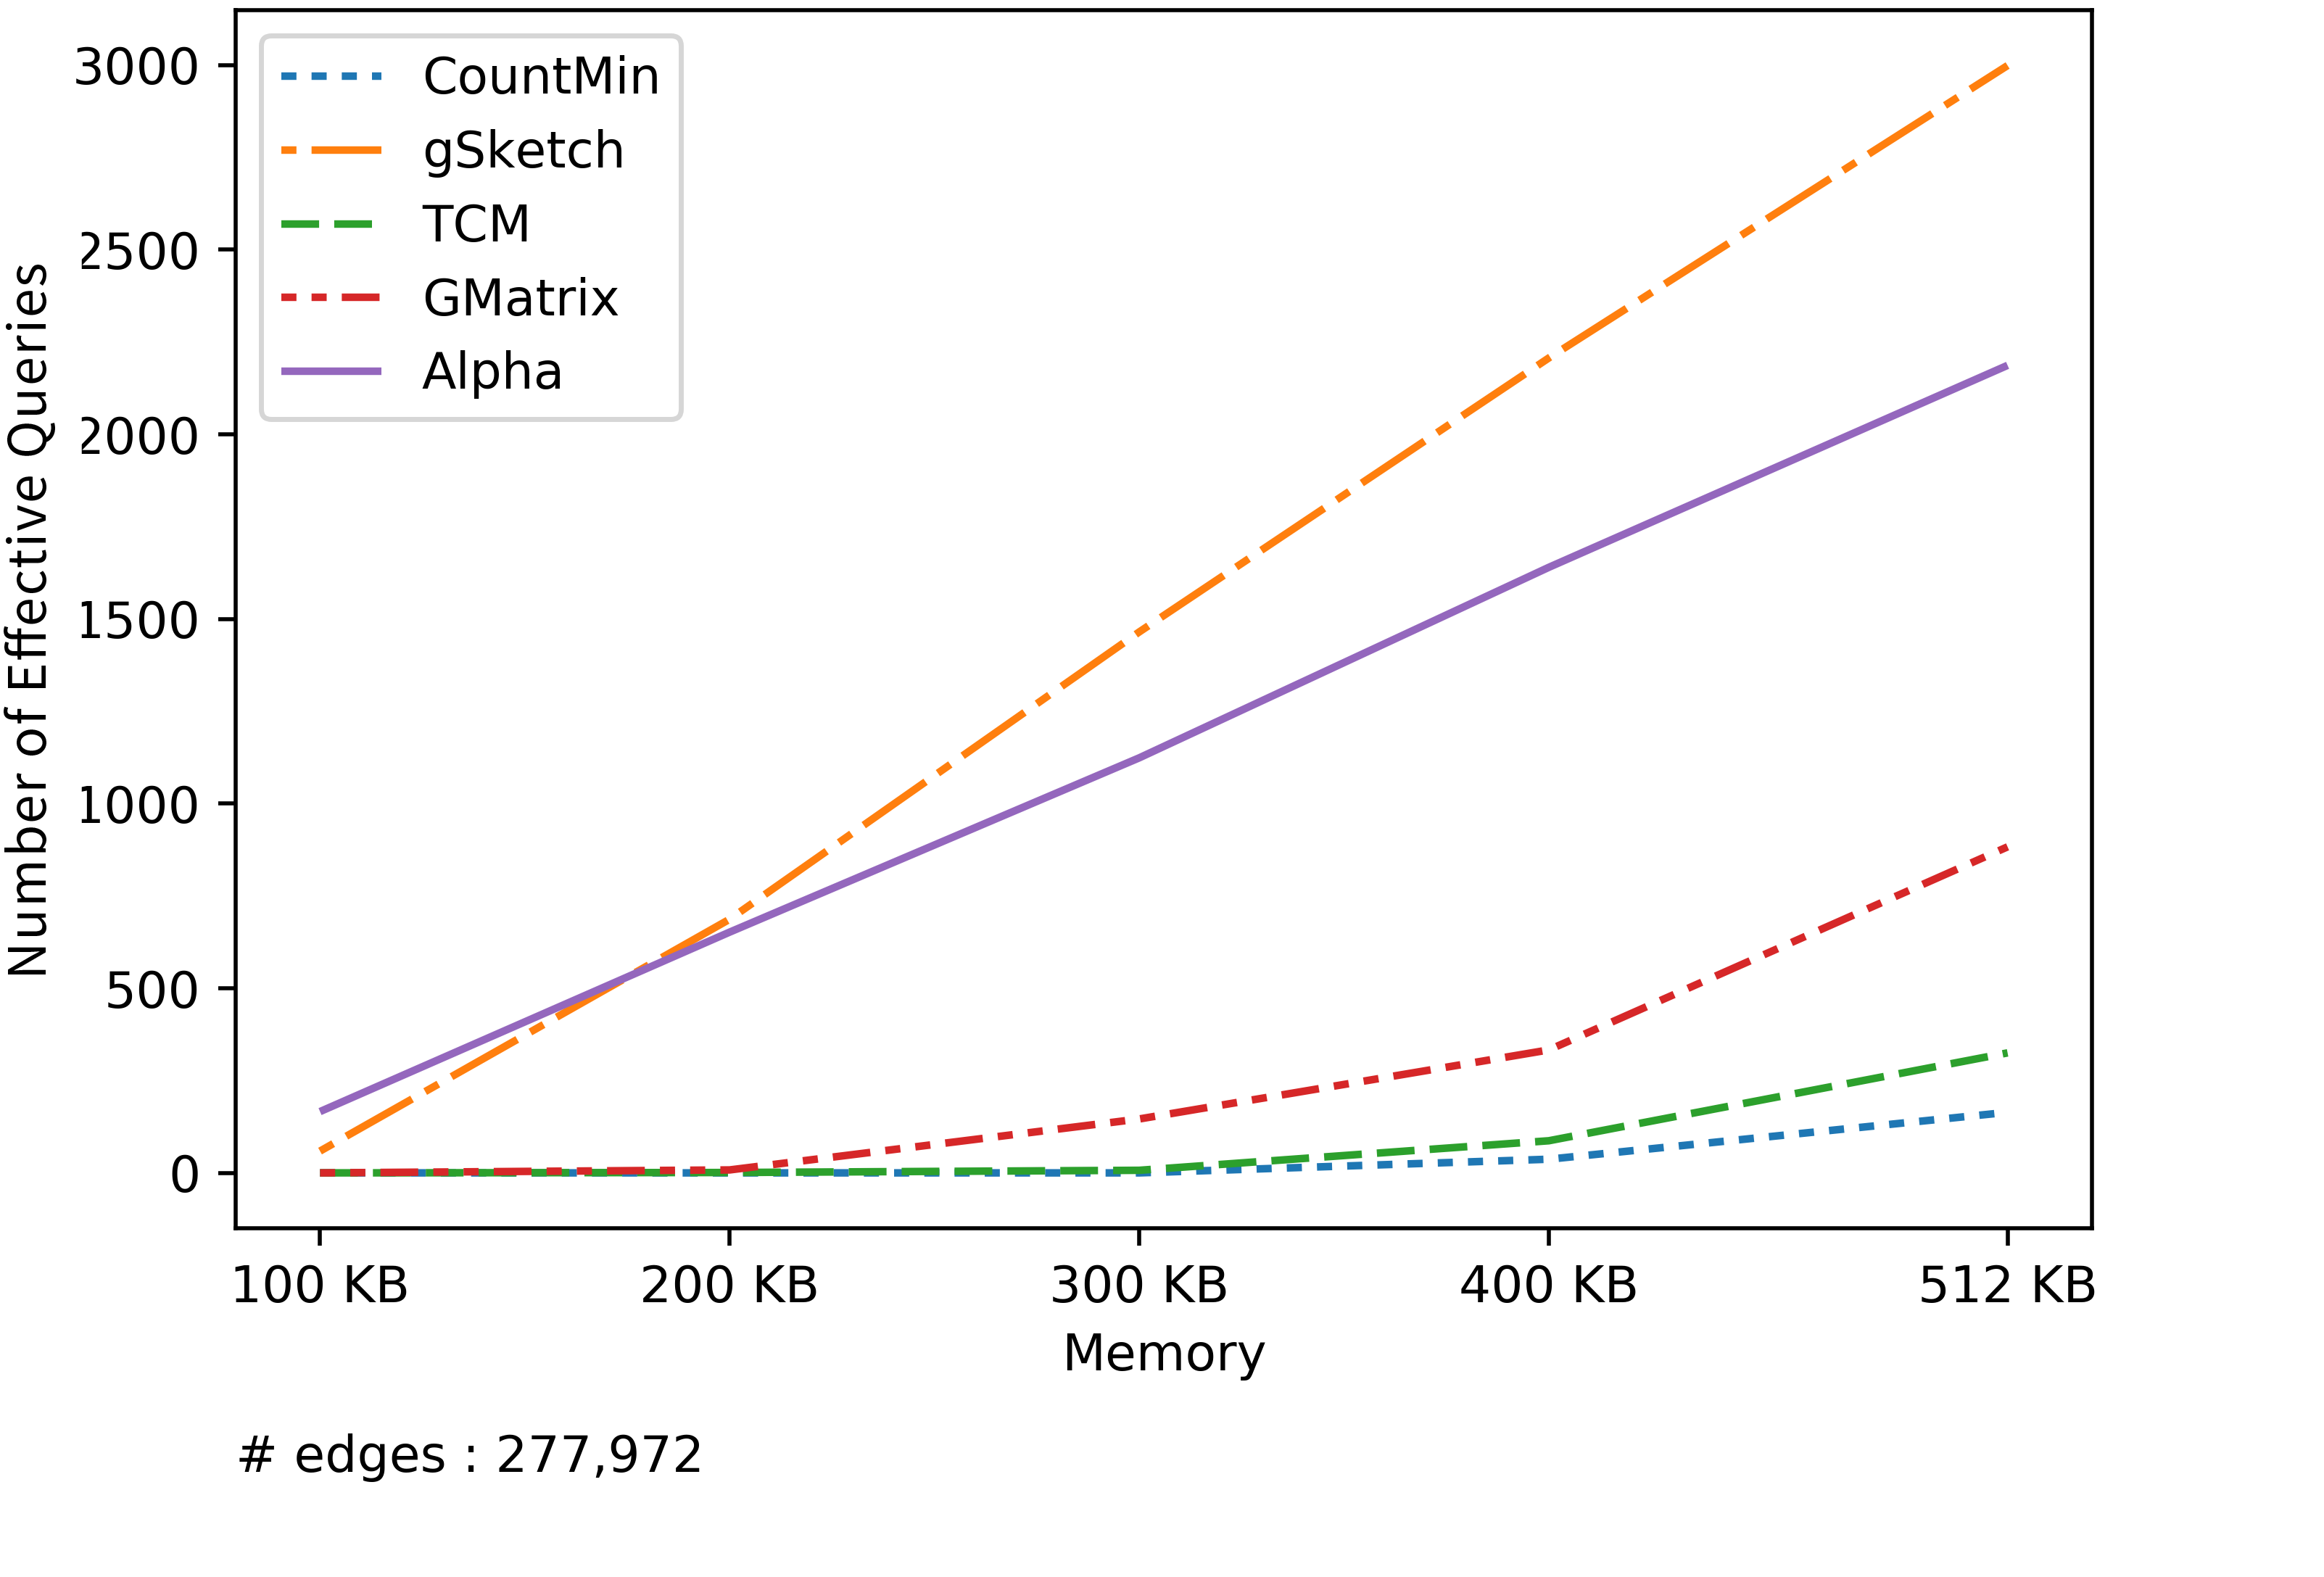
\includegraphics[width=0.85\textwidth]{results/neq/unicorn-wget-neq}
    \vspace{-0.5cm}
    \caption{Number of effective queries vs Memory for unicorn-wget dataset}
    \label{fig:unicorn-wget-neq}
\end{figure}

\begin{figure}[H]
    \centering 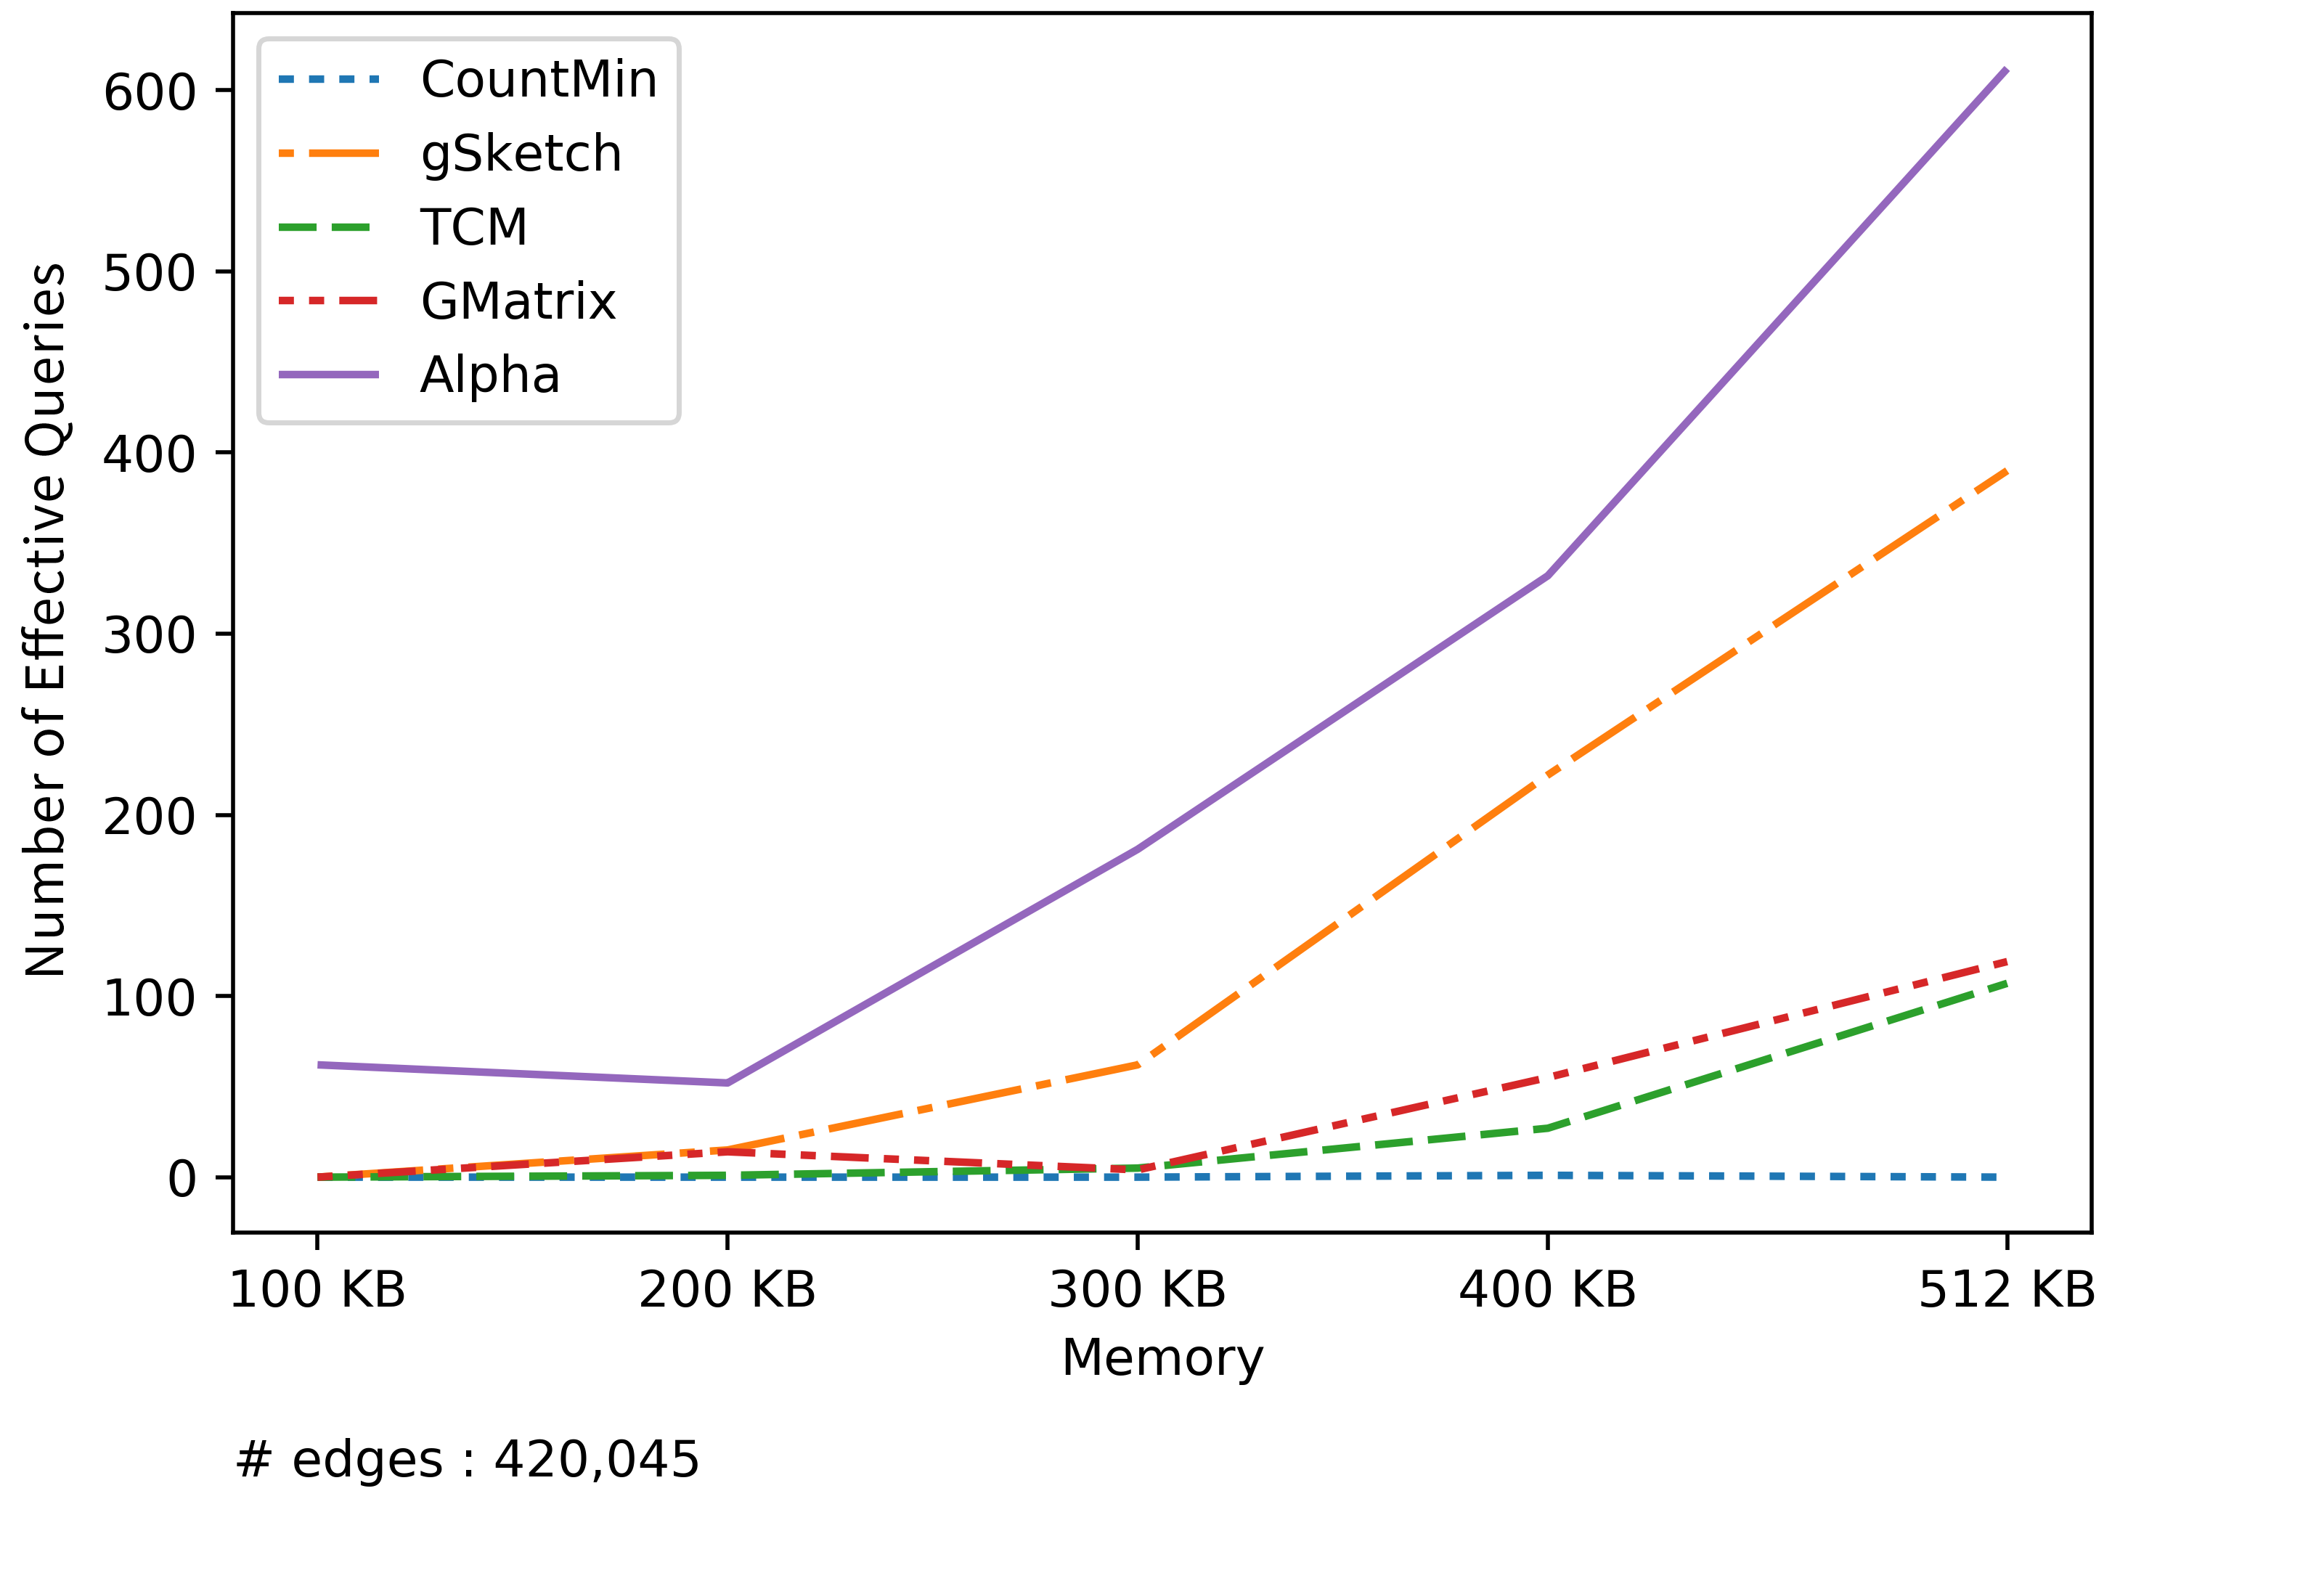
\includegraphics[width=0.85\textwidth]{results/neq/email-EuAll-neq}
    \vspace{-0.5cm}
    \caption{Number of effective queries vs Memory for email-EuAll dataset}
    \label{fig:email-EuAll-neq}
\end{figure}

\begin{figure}[H]
    \centering 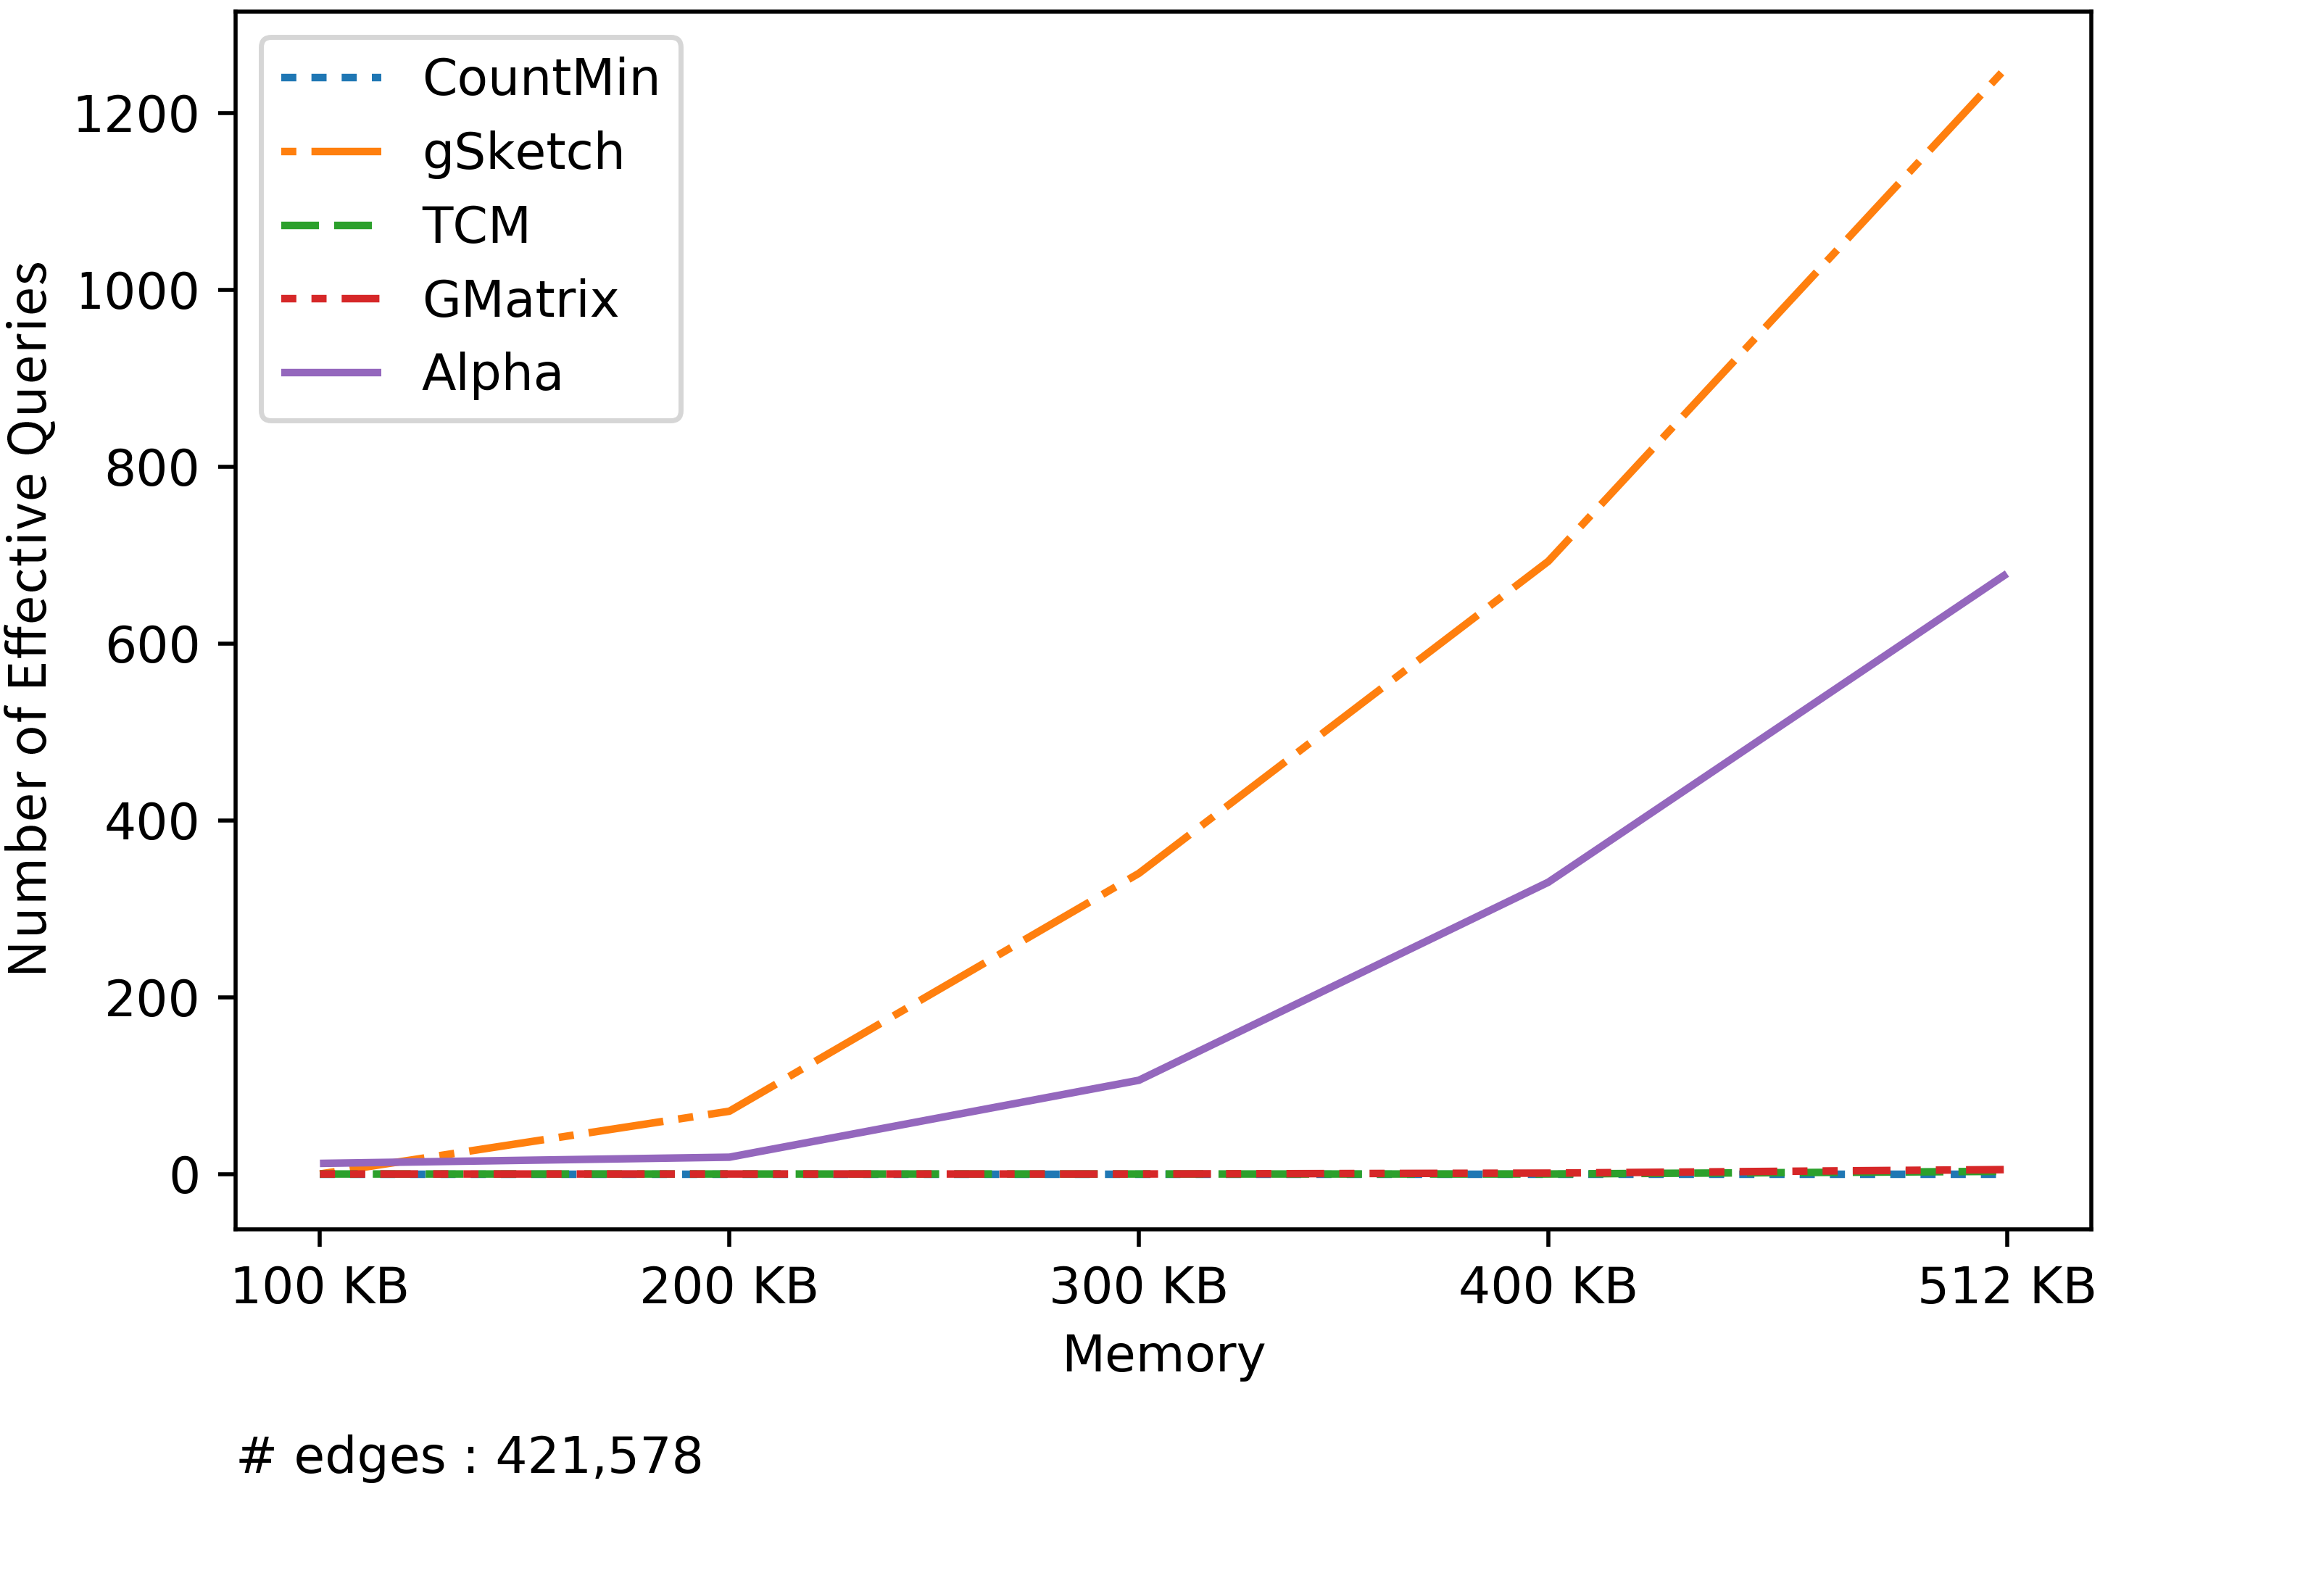
\includegraphics[width=0.85\textwidth]{results/neq/cit-HepPh-neq}
    \vspace{-0.5cm}
    \caption{Number of effective queries vs Memory for cit-HepPh dataset}
    \label{fig:cit-HepPh-neq}
\end{figure}

\begin{figure}[H]
    \centering 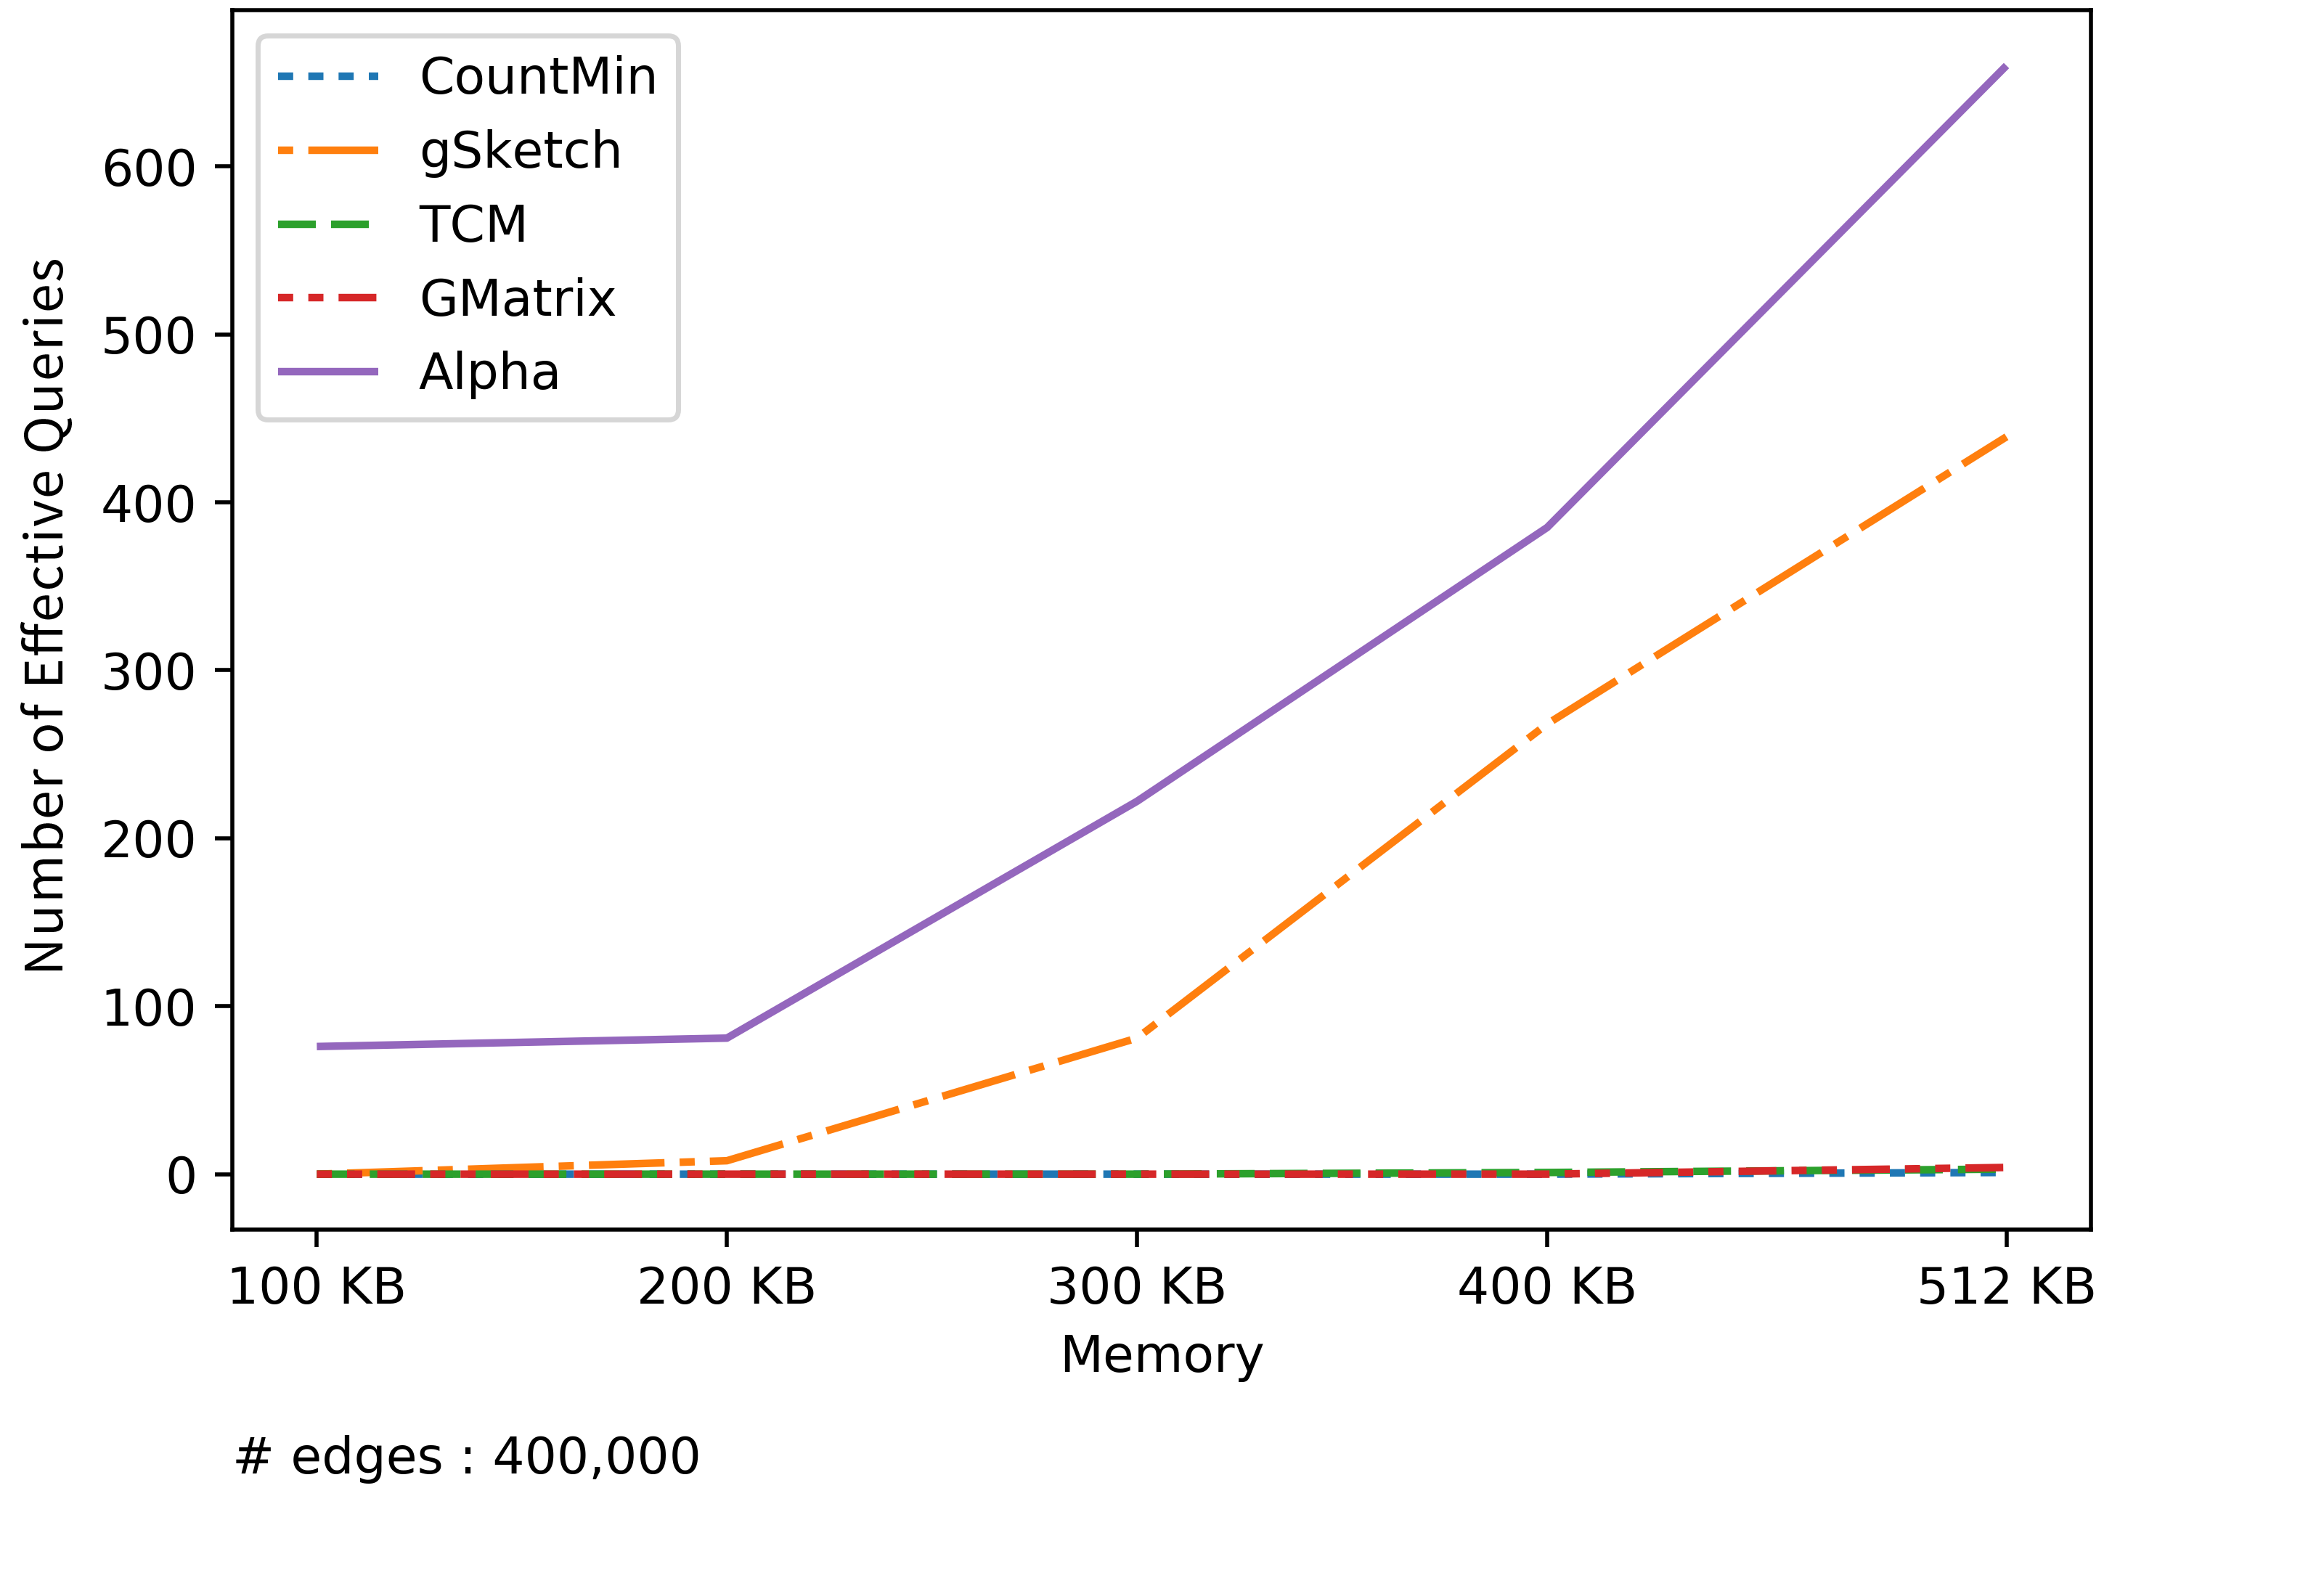
\includegraphics[width=0.85\textwidth]{results/neq/gen-scale-free-neq}
    \vspace{-0.5cm}
    \caption{Number of effective queries vs Memory for gen-scale-free dataset}
    \label{fig:gen-scale-free-neq}
\end{figure}

\begin{figure}[H]
    \centering 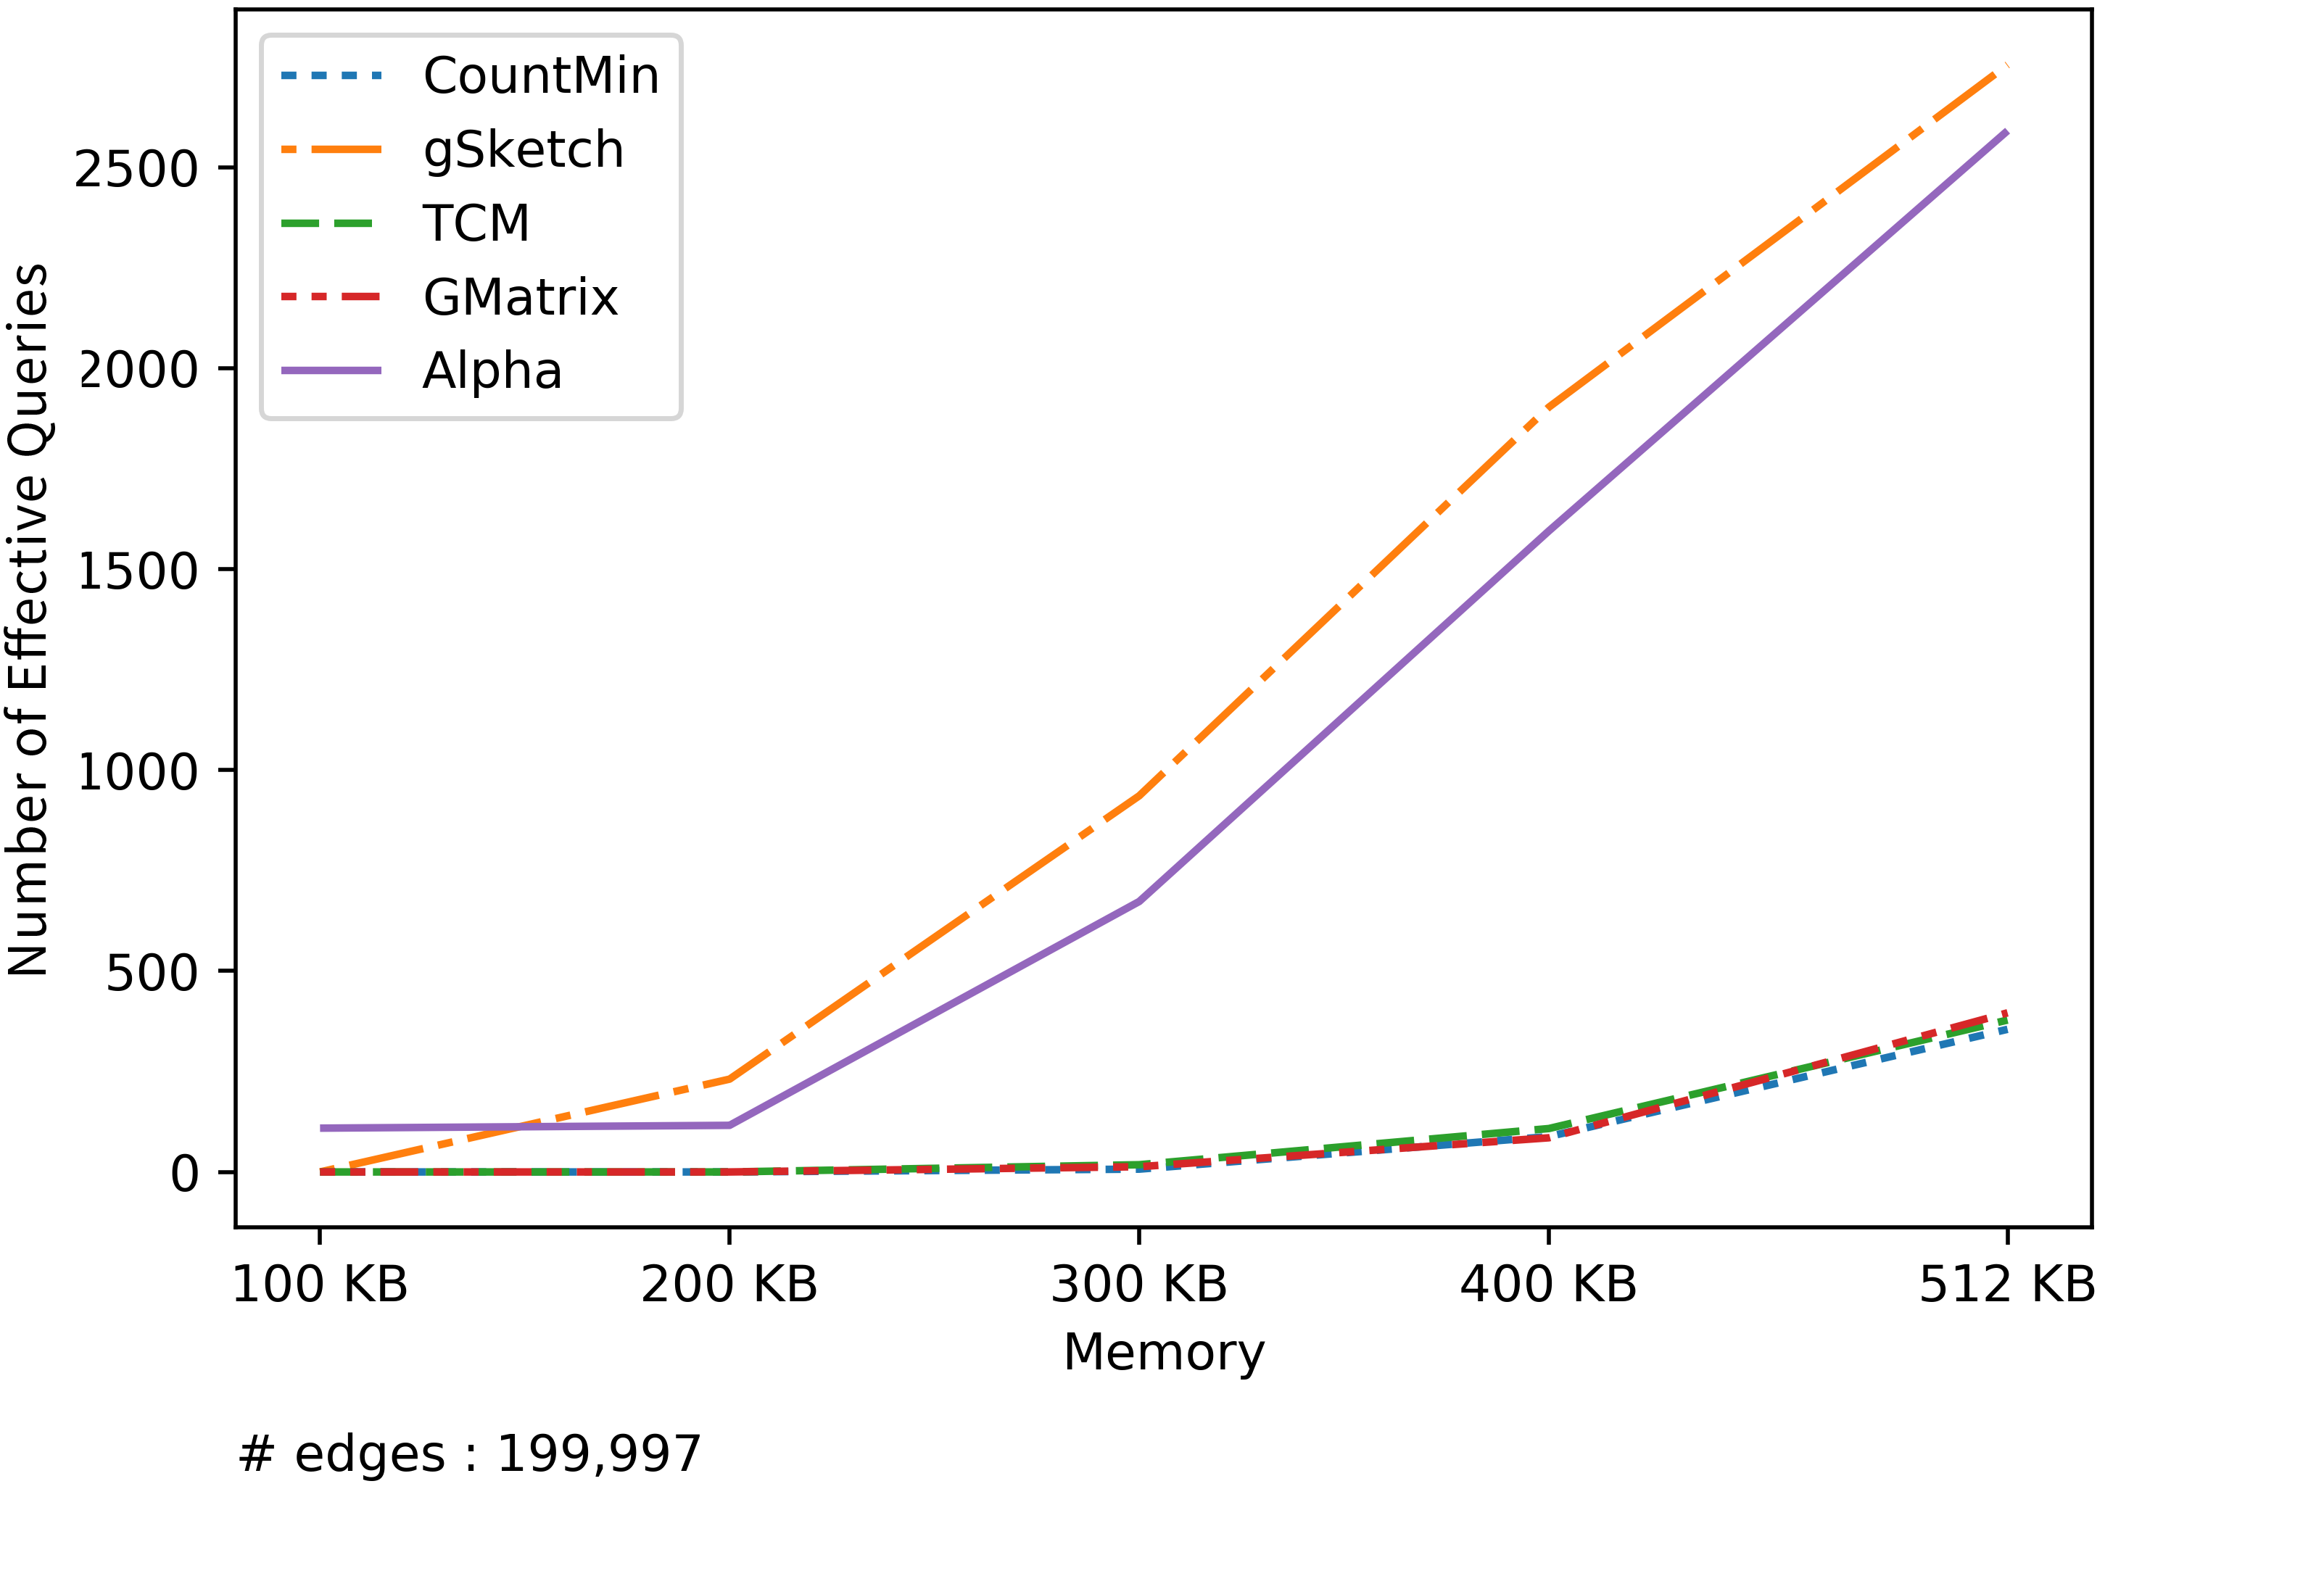
\includegraphics[width=0.85\textwidth]{results/neq/gen-small-world-neq}
    \vspace{-0.5cm}
    \caption{Number of effective queries vs Memory for gen-small-world dataset}
    \label{fig:gen-small-world-neq}
\end{figure}

\subsection*{Observations and inferences}

\paragraph{}
The number of effective queries for each sketch was calculated by querying the sketches against 10,000 edges, which were chosen through reservoir sampling from the original dataset. 

\paragraph{}
In the results for the datasets, unicorn-wget in \autoref{fig:unicorn-wget-neq}, cit-HepPh in \autoref{fig:cit-HepPh-neq} and gen-small-world in \autoref{fig:gen-small-world-neq}; Alpha has a significantly higher number of effective queries in general than all the other sketches except for gSketch.

\paragraph{}
Alpha has surpassed the accuracy of gSketch for email-EuAll in \autoref{fig:email-EuAll-neq} and gen-scale-free in \autoref{fig:gen-scale-free-neq}. 

\paragraph{}
All the sketches for the tested datasets have produced poor accuracies. The unicorn-wget dataset shows the highest number of effective queries for the tested datasets. However, even that result has capped around 3,000 effective queries per 10,000 queries in total. It can be inferred that the low accuracy for the datasets has been a result of the higher compression ratio. It is possible to achieve a better accuracy through allocation of more memory for the sketches. 

\paragraph{}
Alpha has a much higher accuracy with regard to number of effective queries in comparison to TCM, GMatrix and CountMin. This is sufficient to prove the superiority of the proposed solution against the existing sketching techniques. 
\section{Heavy nodes}
\label{section:heavy_nodes}

\subsection*{Purpose}

\paragraph{}
To study the inter-accuracy of top-k heavy nodes between the original stream and the graph sketches.

\paragraph{}
Inter-accuracy for top-k elements has been defined in \autoref{section:metrics_inter}.

\subsection*{Results}

\begin{figure}[H]
    \centering 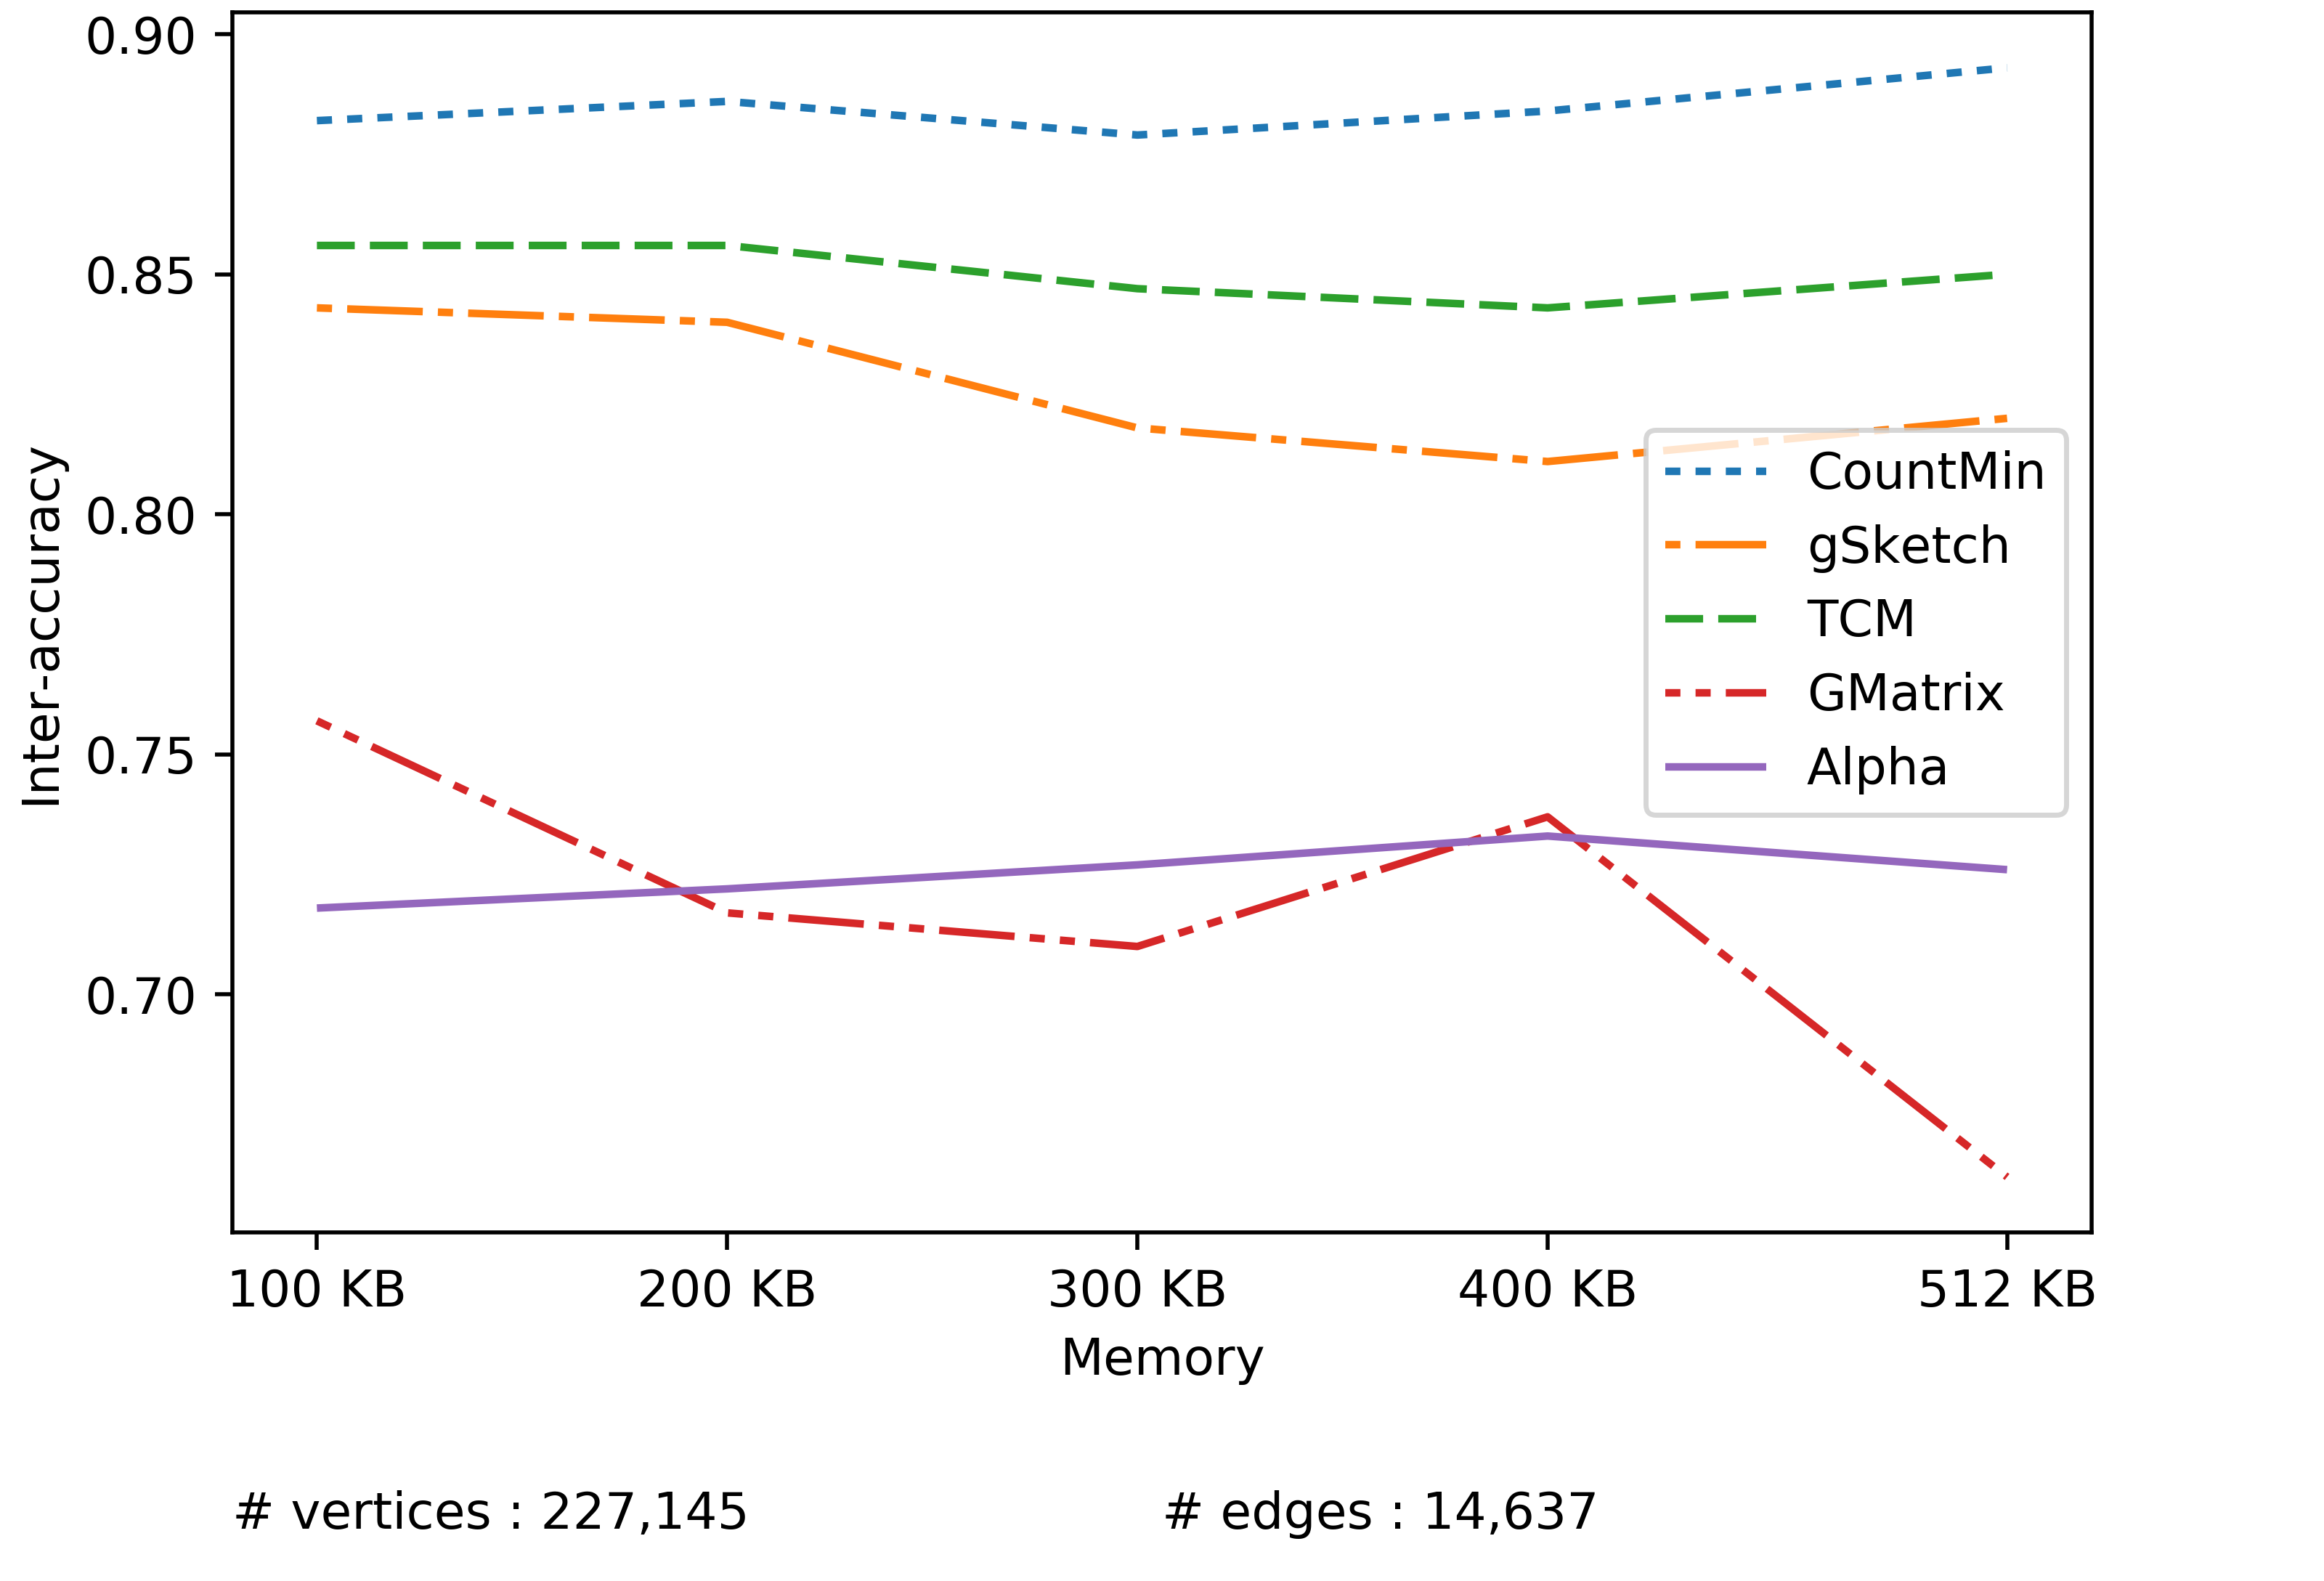
\includegraphics[width=0.85\textwidth]{results/hn/unicorn-wget-hn}
    \vspace{-0.5cm}
    \caption{Inter accuracy of heavy nodes vs Memory for unicorn-wget dataset}
    \label{fig:unicorn-wget-hn}
\end{figure}

\begin{figure}[H]
    \centering 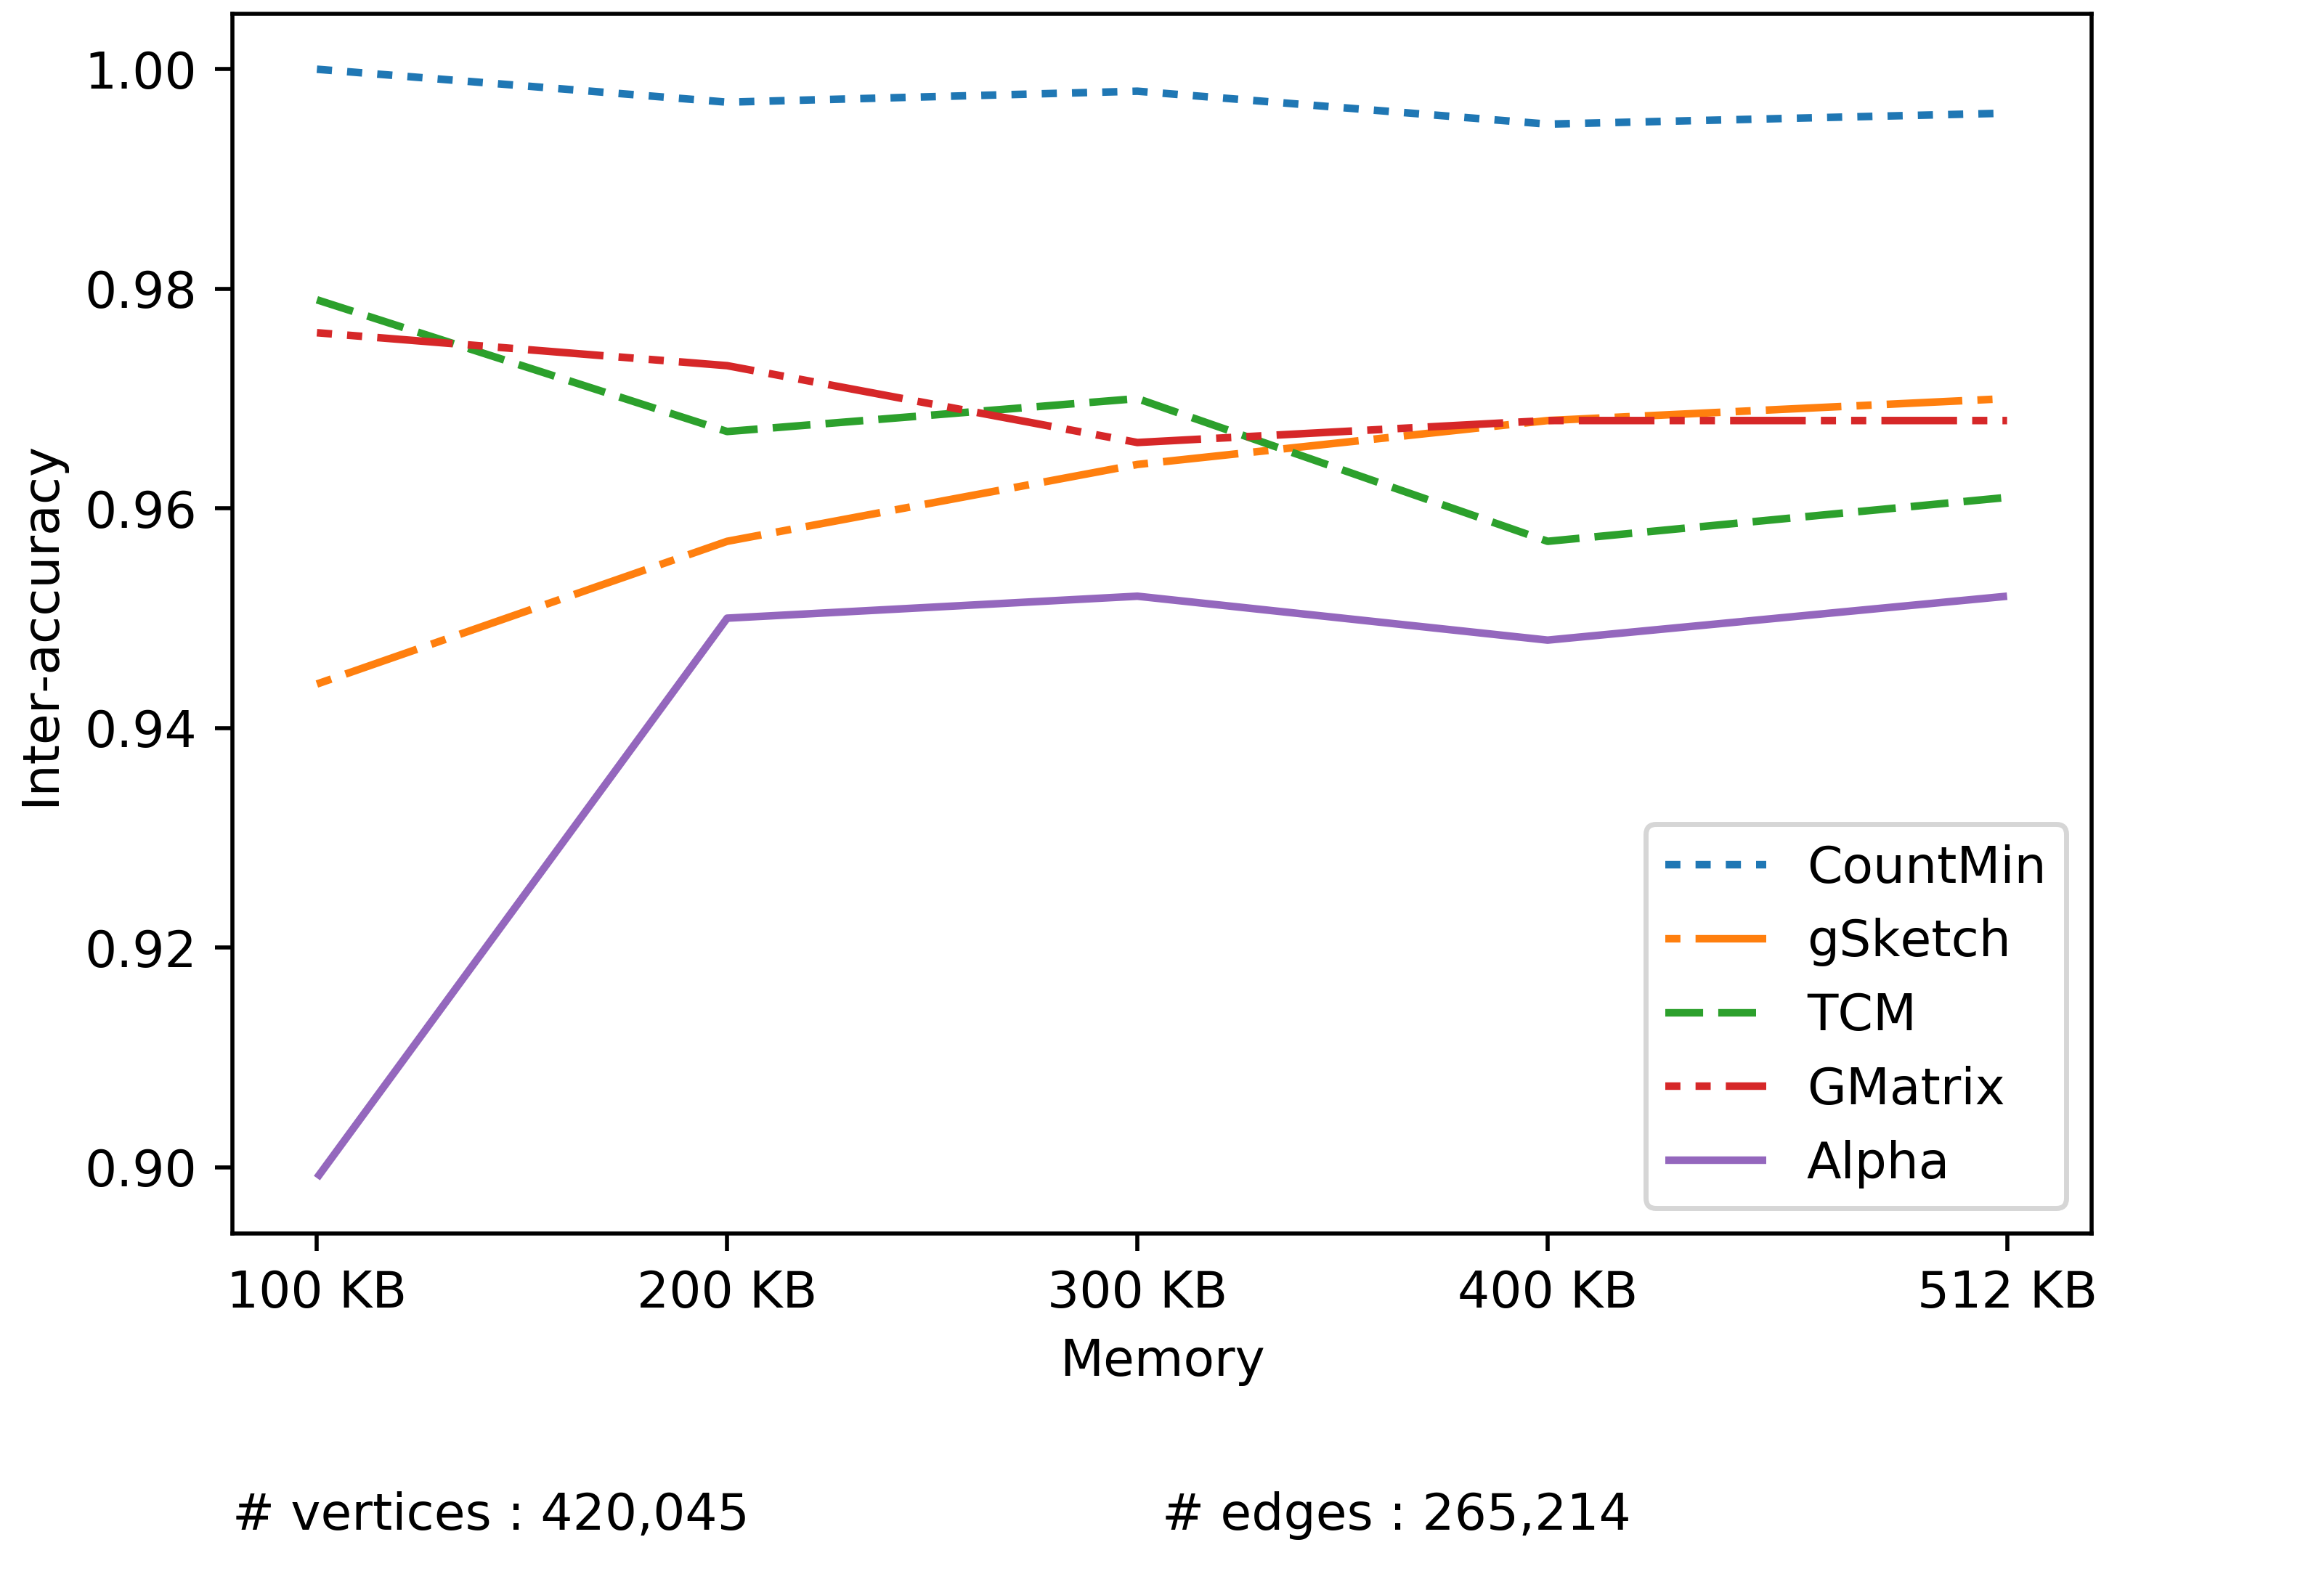
\includegraphics[width=0.85\textwidth]{results/hn/email-EuAll-hn}
    \vspace{-0.5cm}
    \caption{Inter accuracy of heavy nodes vs Memory for email-EuAll dataset}
    \label{fig:email-EuAll-hn}
\end{figure}

\begin{figure}[H]
    \centering 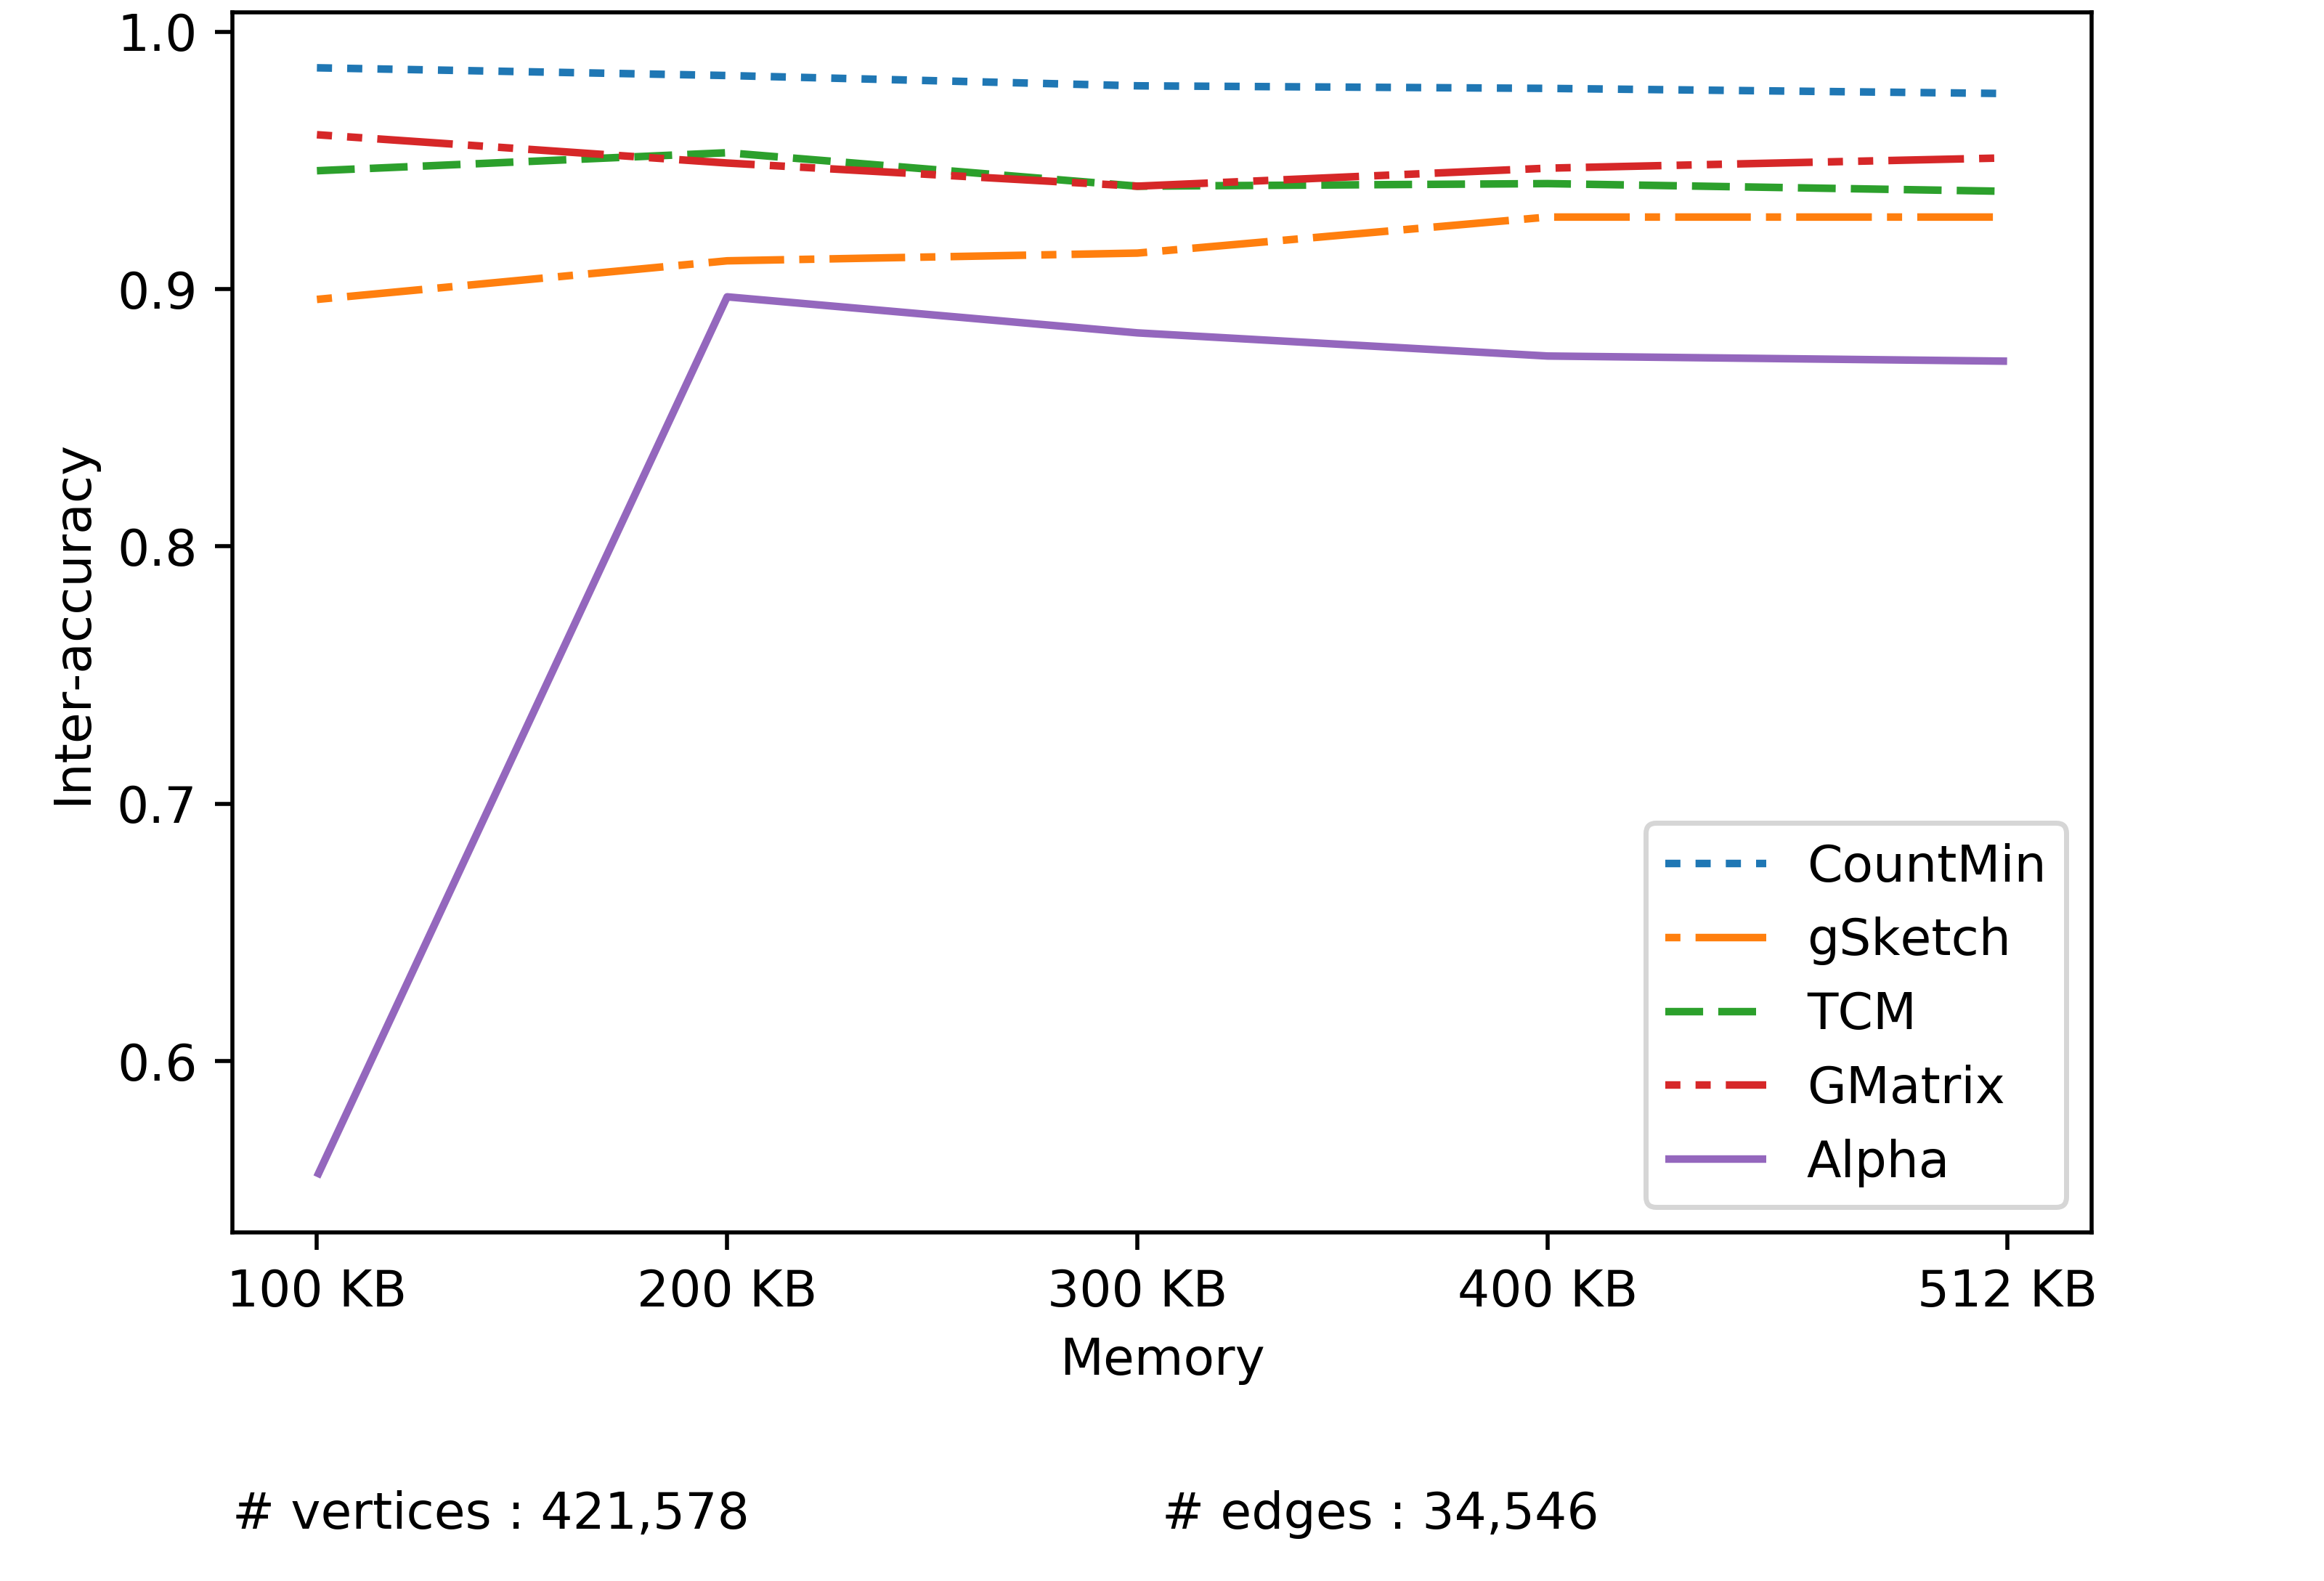
\includegraphics[width=0.85\textwidth]{results/hn/cit-HepPh-hn}
    \vspace{-0.5cm}
    \caption{Inter accuracy of heavy nodes vs Memory for cit-HepPh dataset}
    \label{fig:cit-HepPh-hn}
\end{figure}

\begin{figure}[H]
    \centering 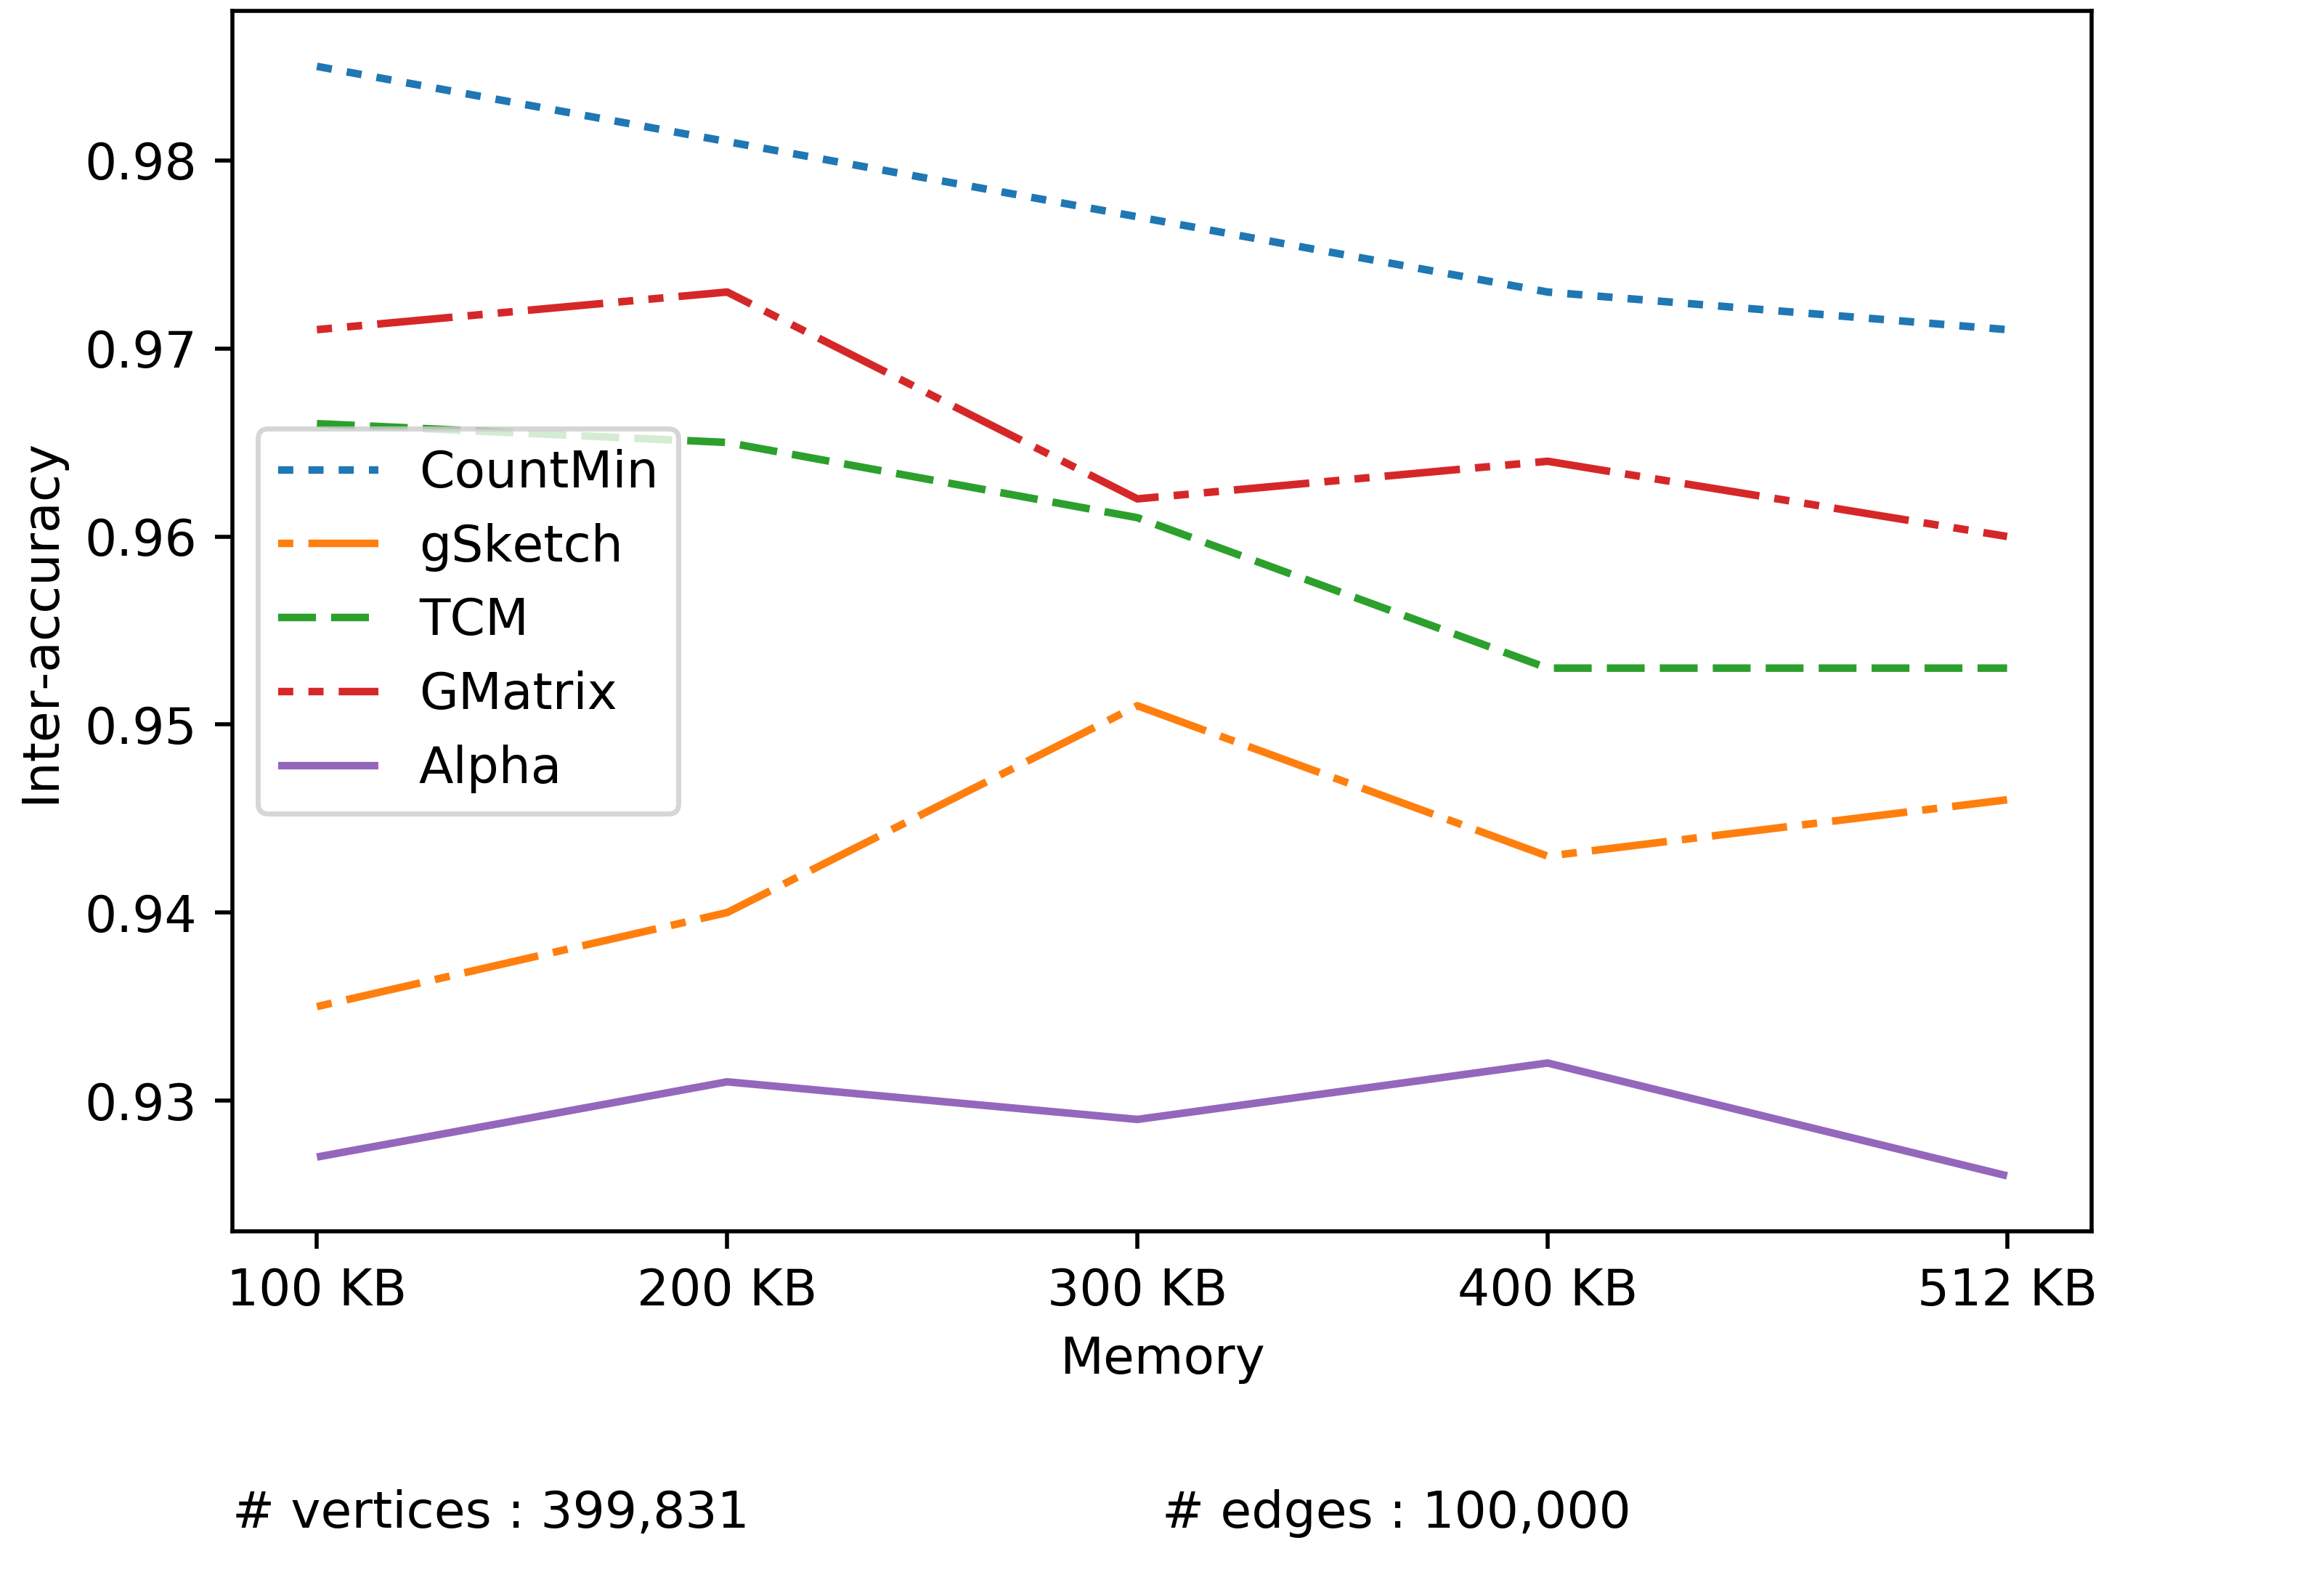
\includegraphics[width=0.85\textwidth]{results/hn/gen-scale-free-hn}
    \vspace{-0.5cm}
    \caption{Inter accuracy of heavy nodes vs Memory for gen-scale-free dataset}
    \label{fig:gen-scale-free-hn}
\end{figure}

\begin{figure}[H]
    \centering 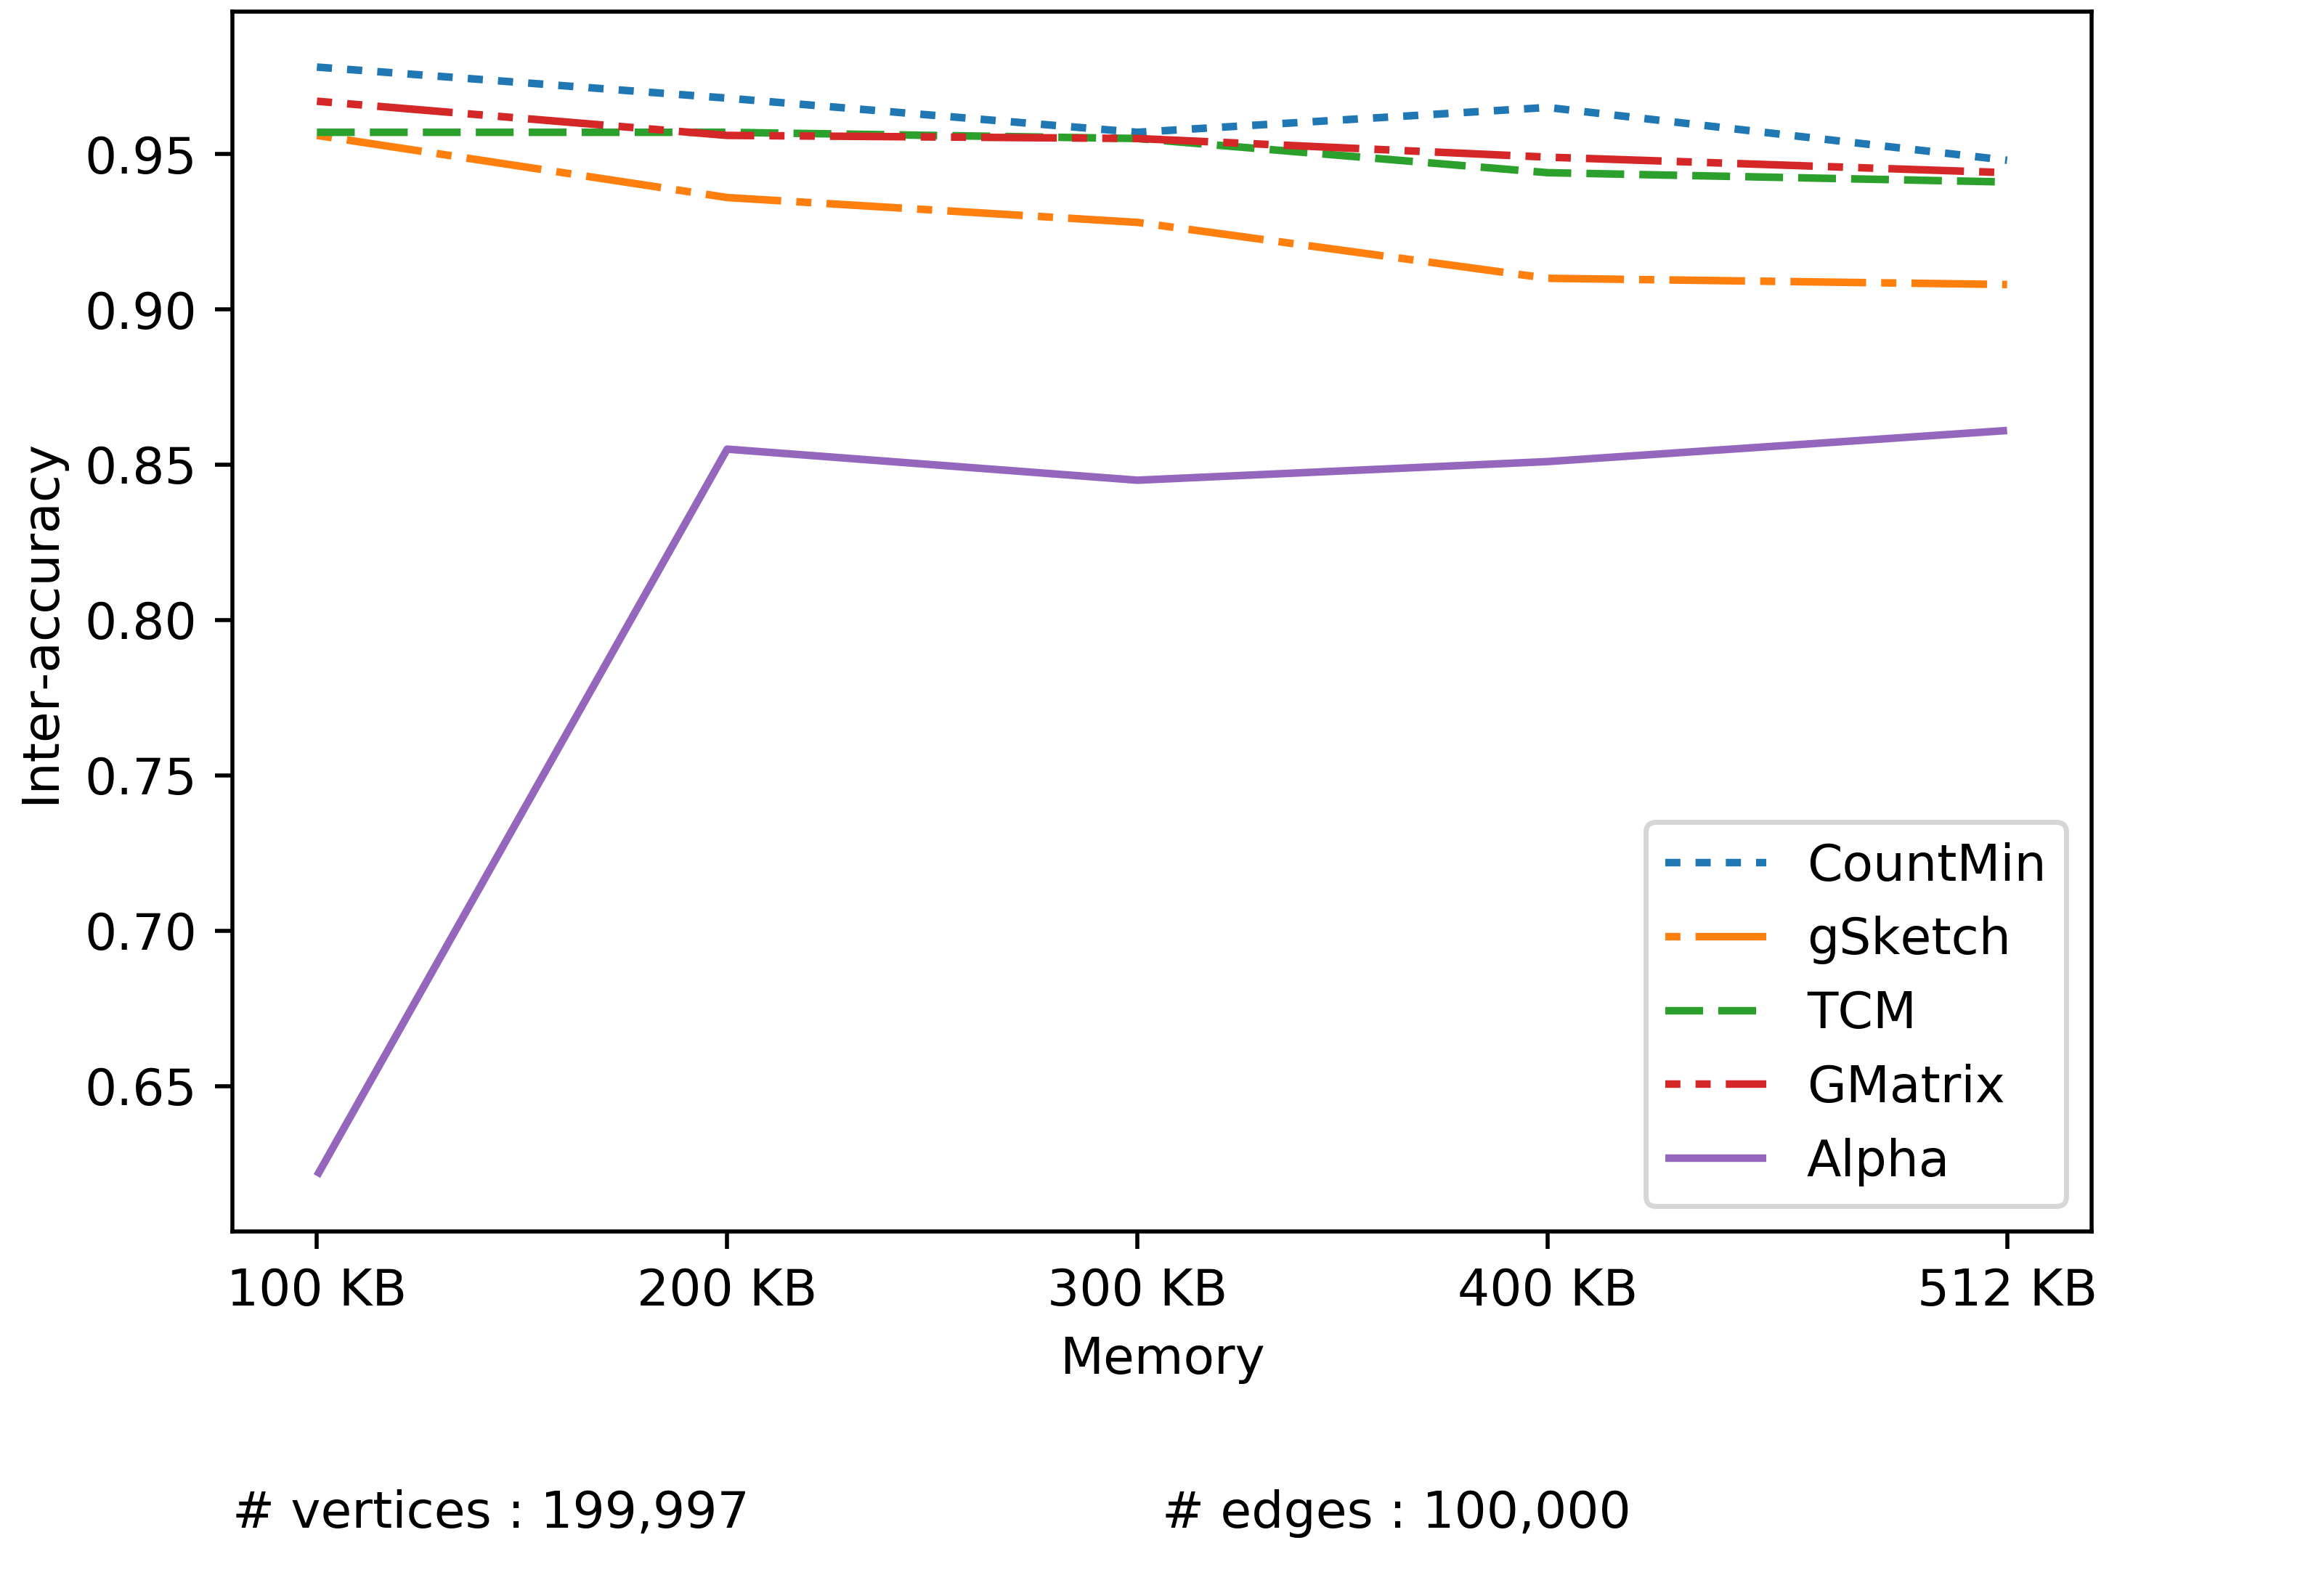
\includegraphics[width=0.85\textwidth]{results/hn/gen-small-world-hn}
    \vspace{-0.5cm}
    \caption{Inter accuracy of heavy nodes vs Memory for gen-small-world dataset}
    \label{fig:gen-small-world-hn}
\end{figure}

\subsection*{Observations and inferences}

\paragraph{}
Both the partitioned sketches, gSketch and Alpha has shown comparably low inter accuracies for top-k heavy node queries for the datasets, unicorn-wget in \autoref{fig:unicorn-wget-hn}, email-EuAll in \autoref{fig:email-EuAll-hn}, cit-HepPh in \autoref{fig:cit-HepPh-hn}, gen-scale-free in \autoref{fig:gen-scale-free-hn} and gen-small-world in \autoref{fig:gen-small-world-hn}. Thus we can infer that the partitioning of the sketches has negatively affected the performance of heavy node queries.

\paragraph{}
CountMin sketch has a higher accuracy for heavy node queries for all the datasets that were tested.

\paragraph{}
The proposed solution Alpha, nor the gSketch are good candidates for heavy node queries. It is evident that the partitioning of the sketches has vastly changed the degree distribution of the original graph, relative to the other sketching techniques. CountMin is best suitable for these types of queries where the heavy node status of the initial graph stream must be preserved.
\section{Heavy edges}
\label{section:heavy_edges}

\subsection*{Purpose}

\paragraph{}
To study the inter-accuracy of top-k heavy edges between the original stream and the graph sketches.

\paragraph{}
Inter-accuracy for top-k elements has been defined in \autoref{section:metrics_inter}.

\subsection*{Results}

\begin{figure}[H]
    \centering 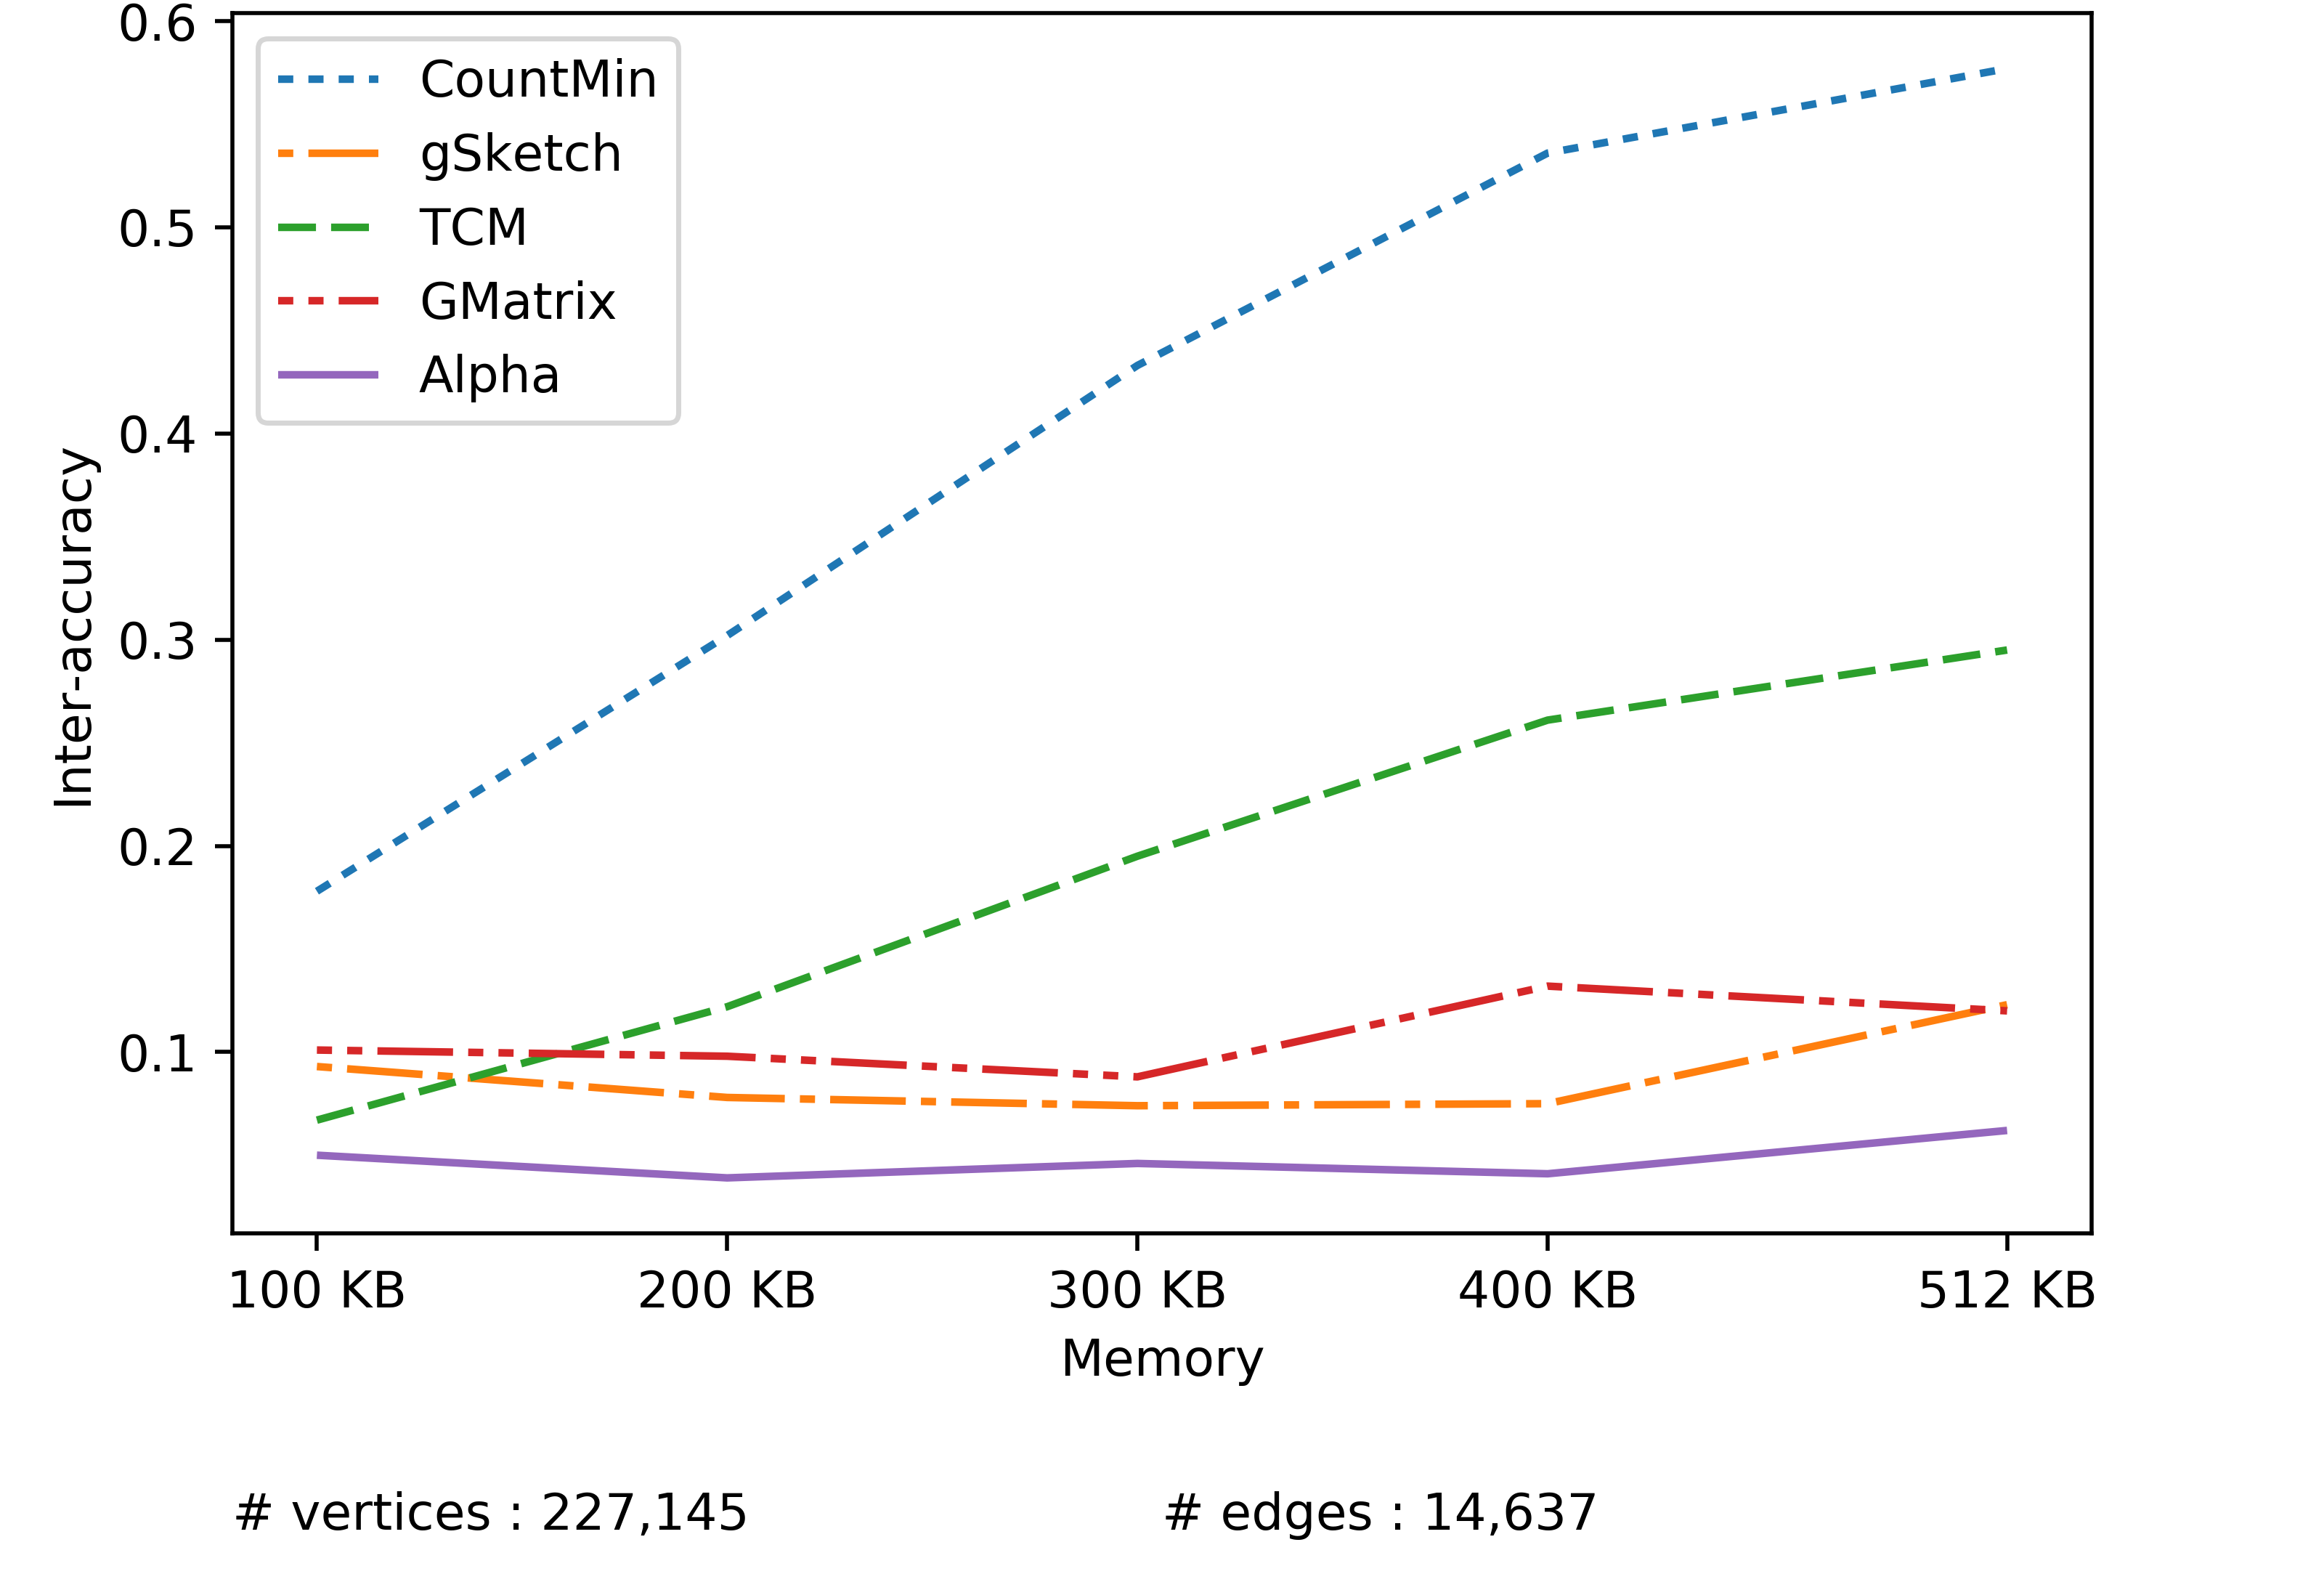
\includegraphics[width=0.85\textwidth]{results/he/unicorn-wget-he}
    \vspace{-0.5cm}
    \caption{Inter accuracy of heavy edges vs Memory for unicorn-wget dataset}
    \label{fig:unicorn-wget-he}
\end{figure}

\begin{figure}[H]
    \centering 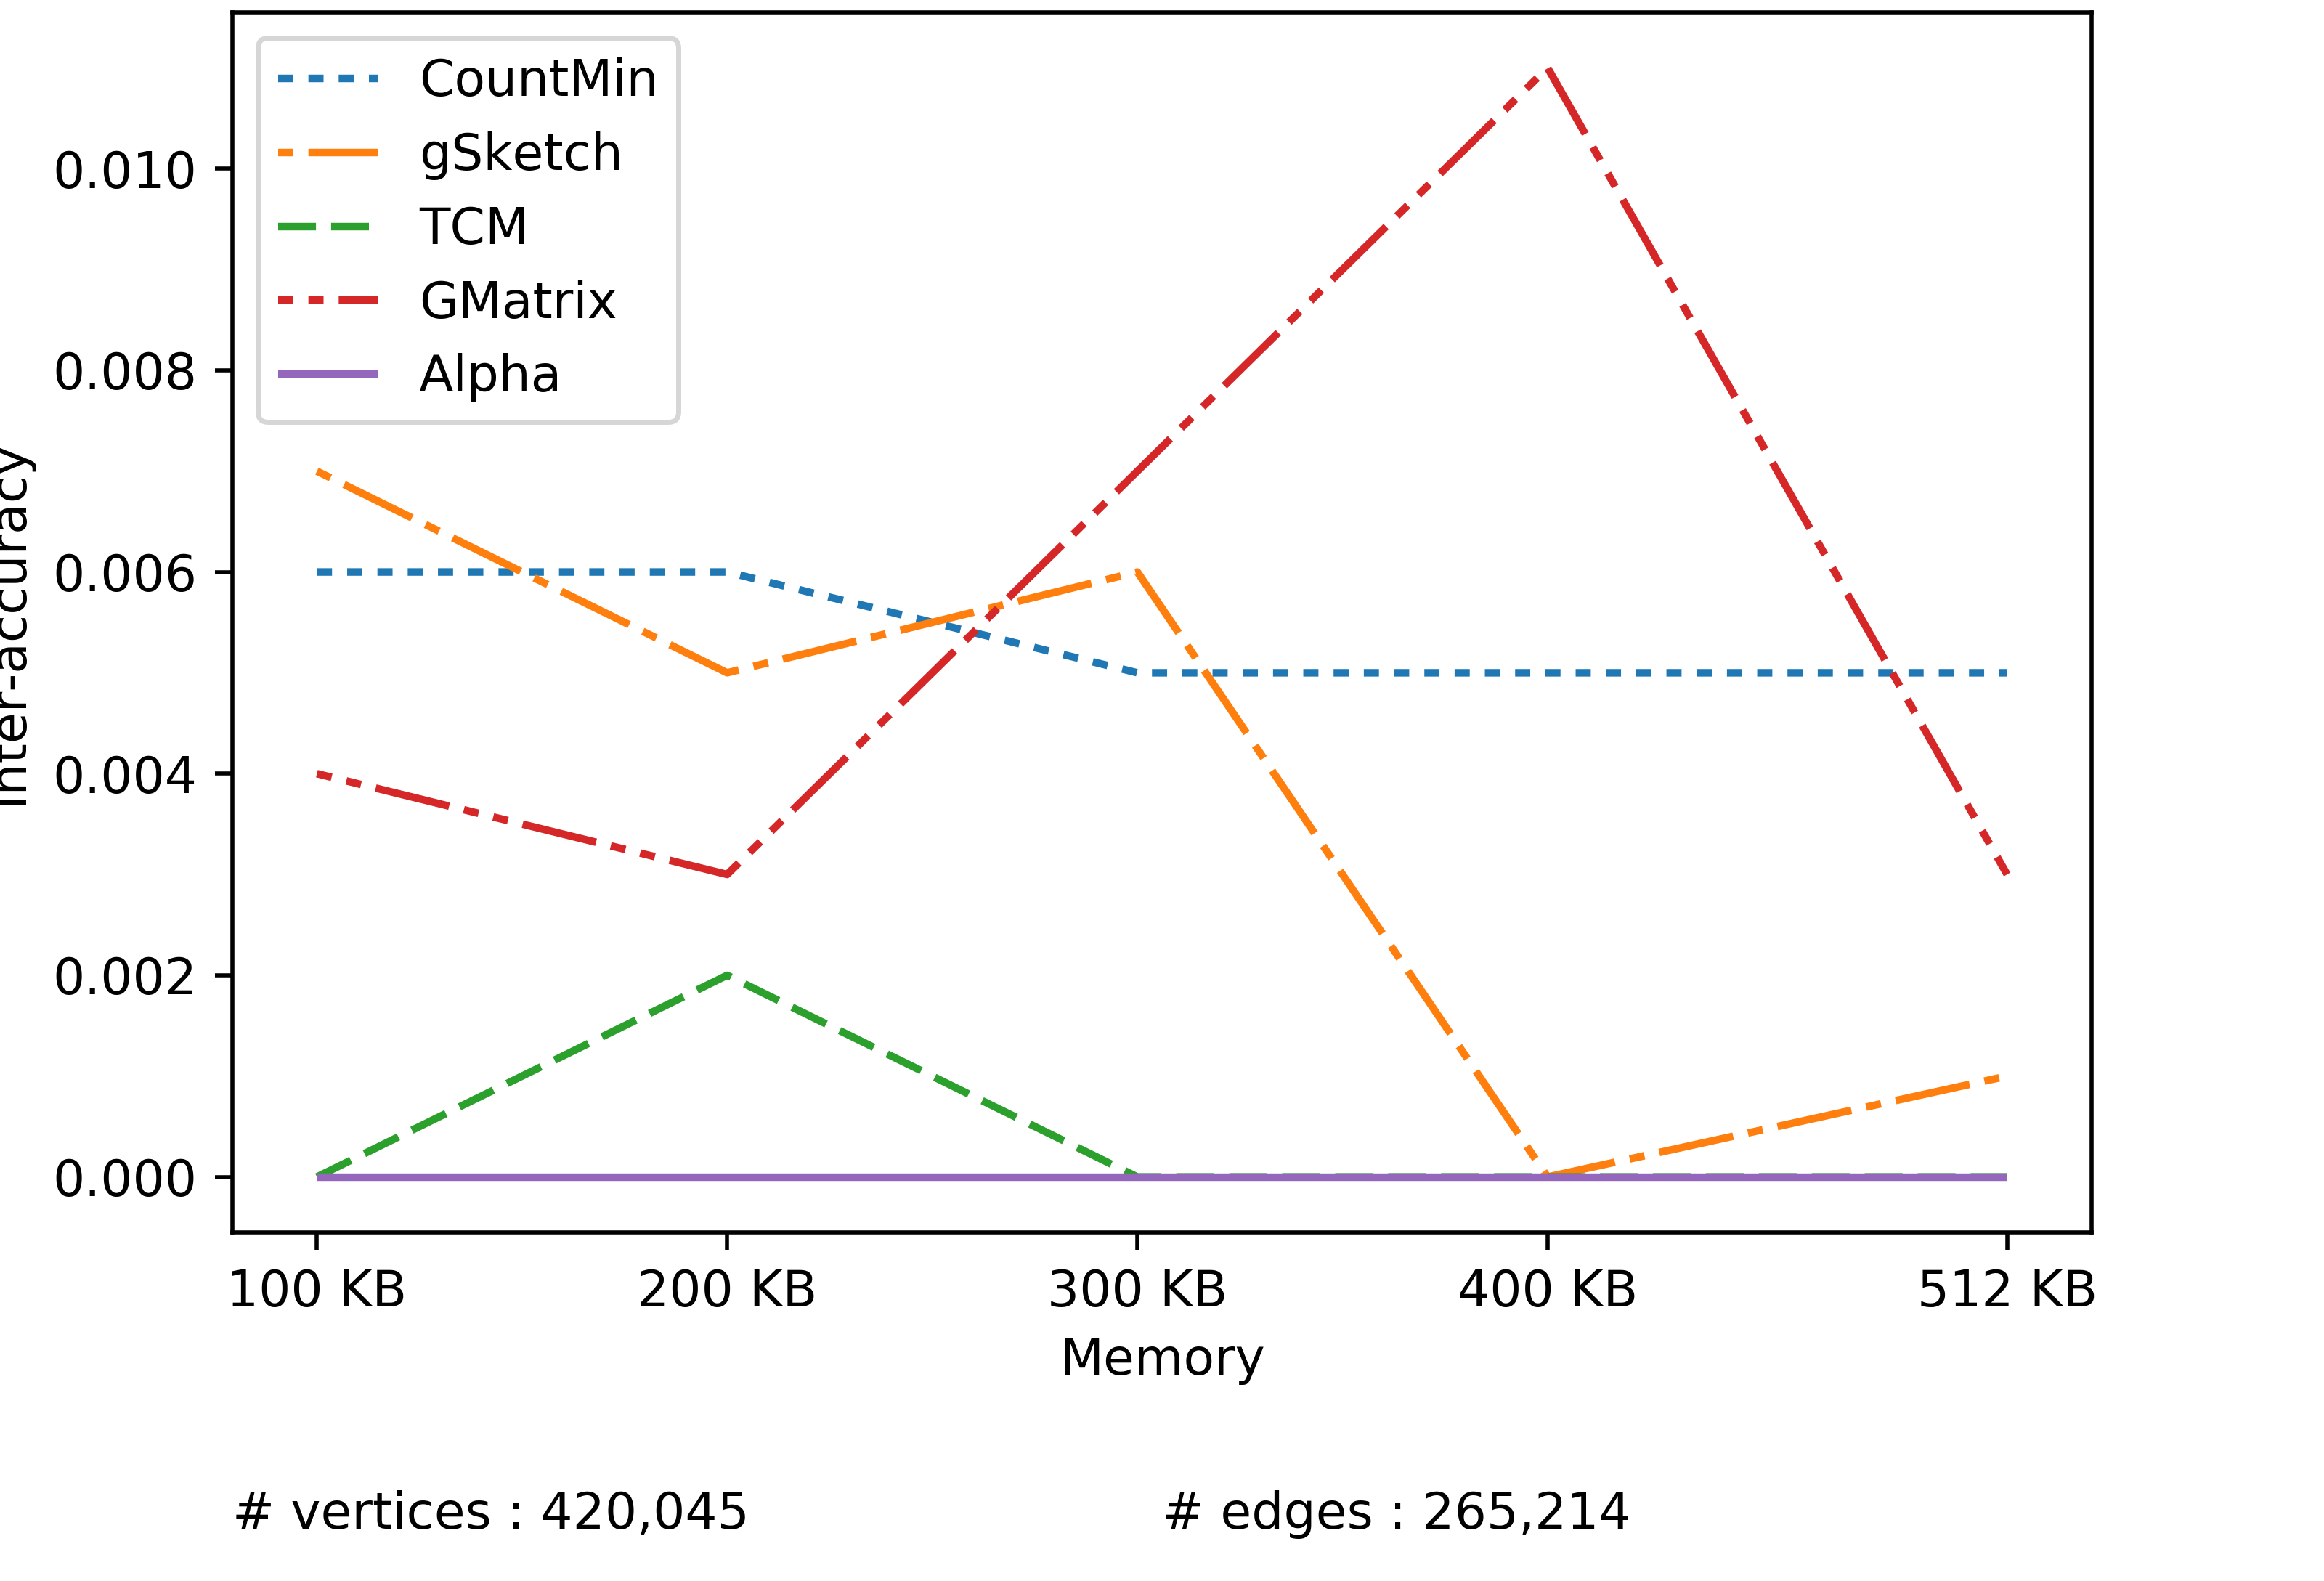
\includegraphics[width=0.85\textwidth]{results/he/email-EuAll-he}
    \vspace{-0.5cm}
    \caption{Inter accuracy of heavy edges vs Memory for email-EuAll dataset}
    \label{fig:email-EuAll-he}
\end{figure}

\begin{figure}[H]
    \centering 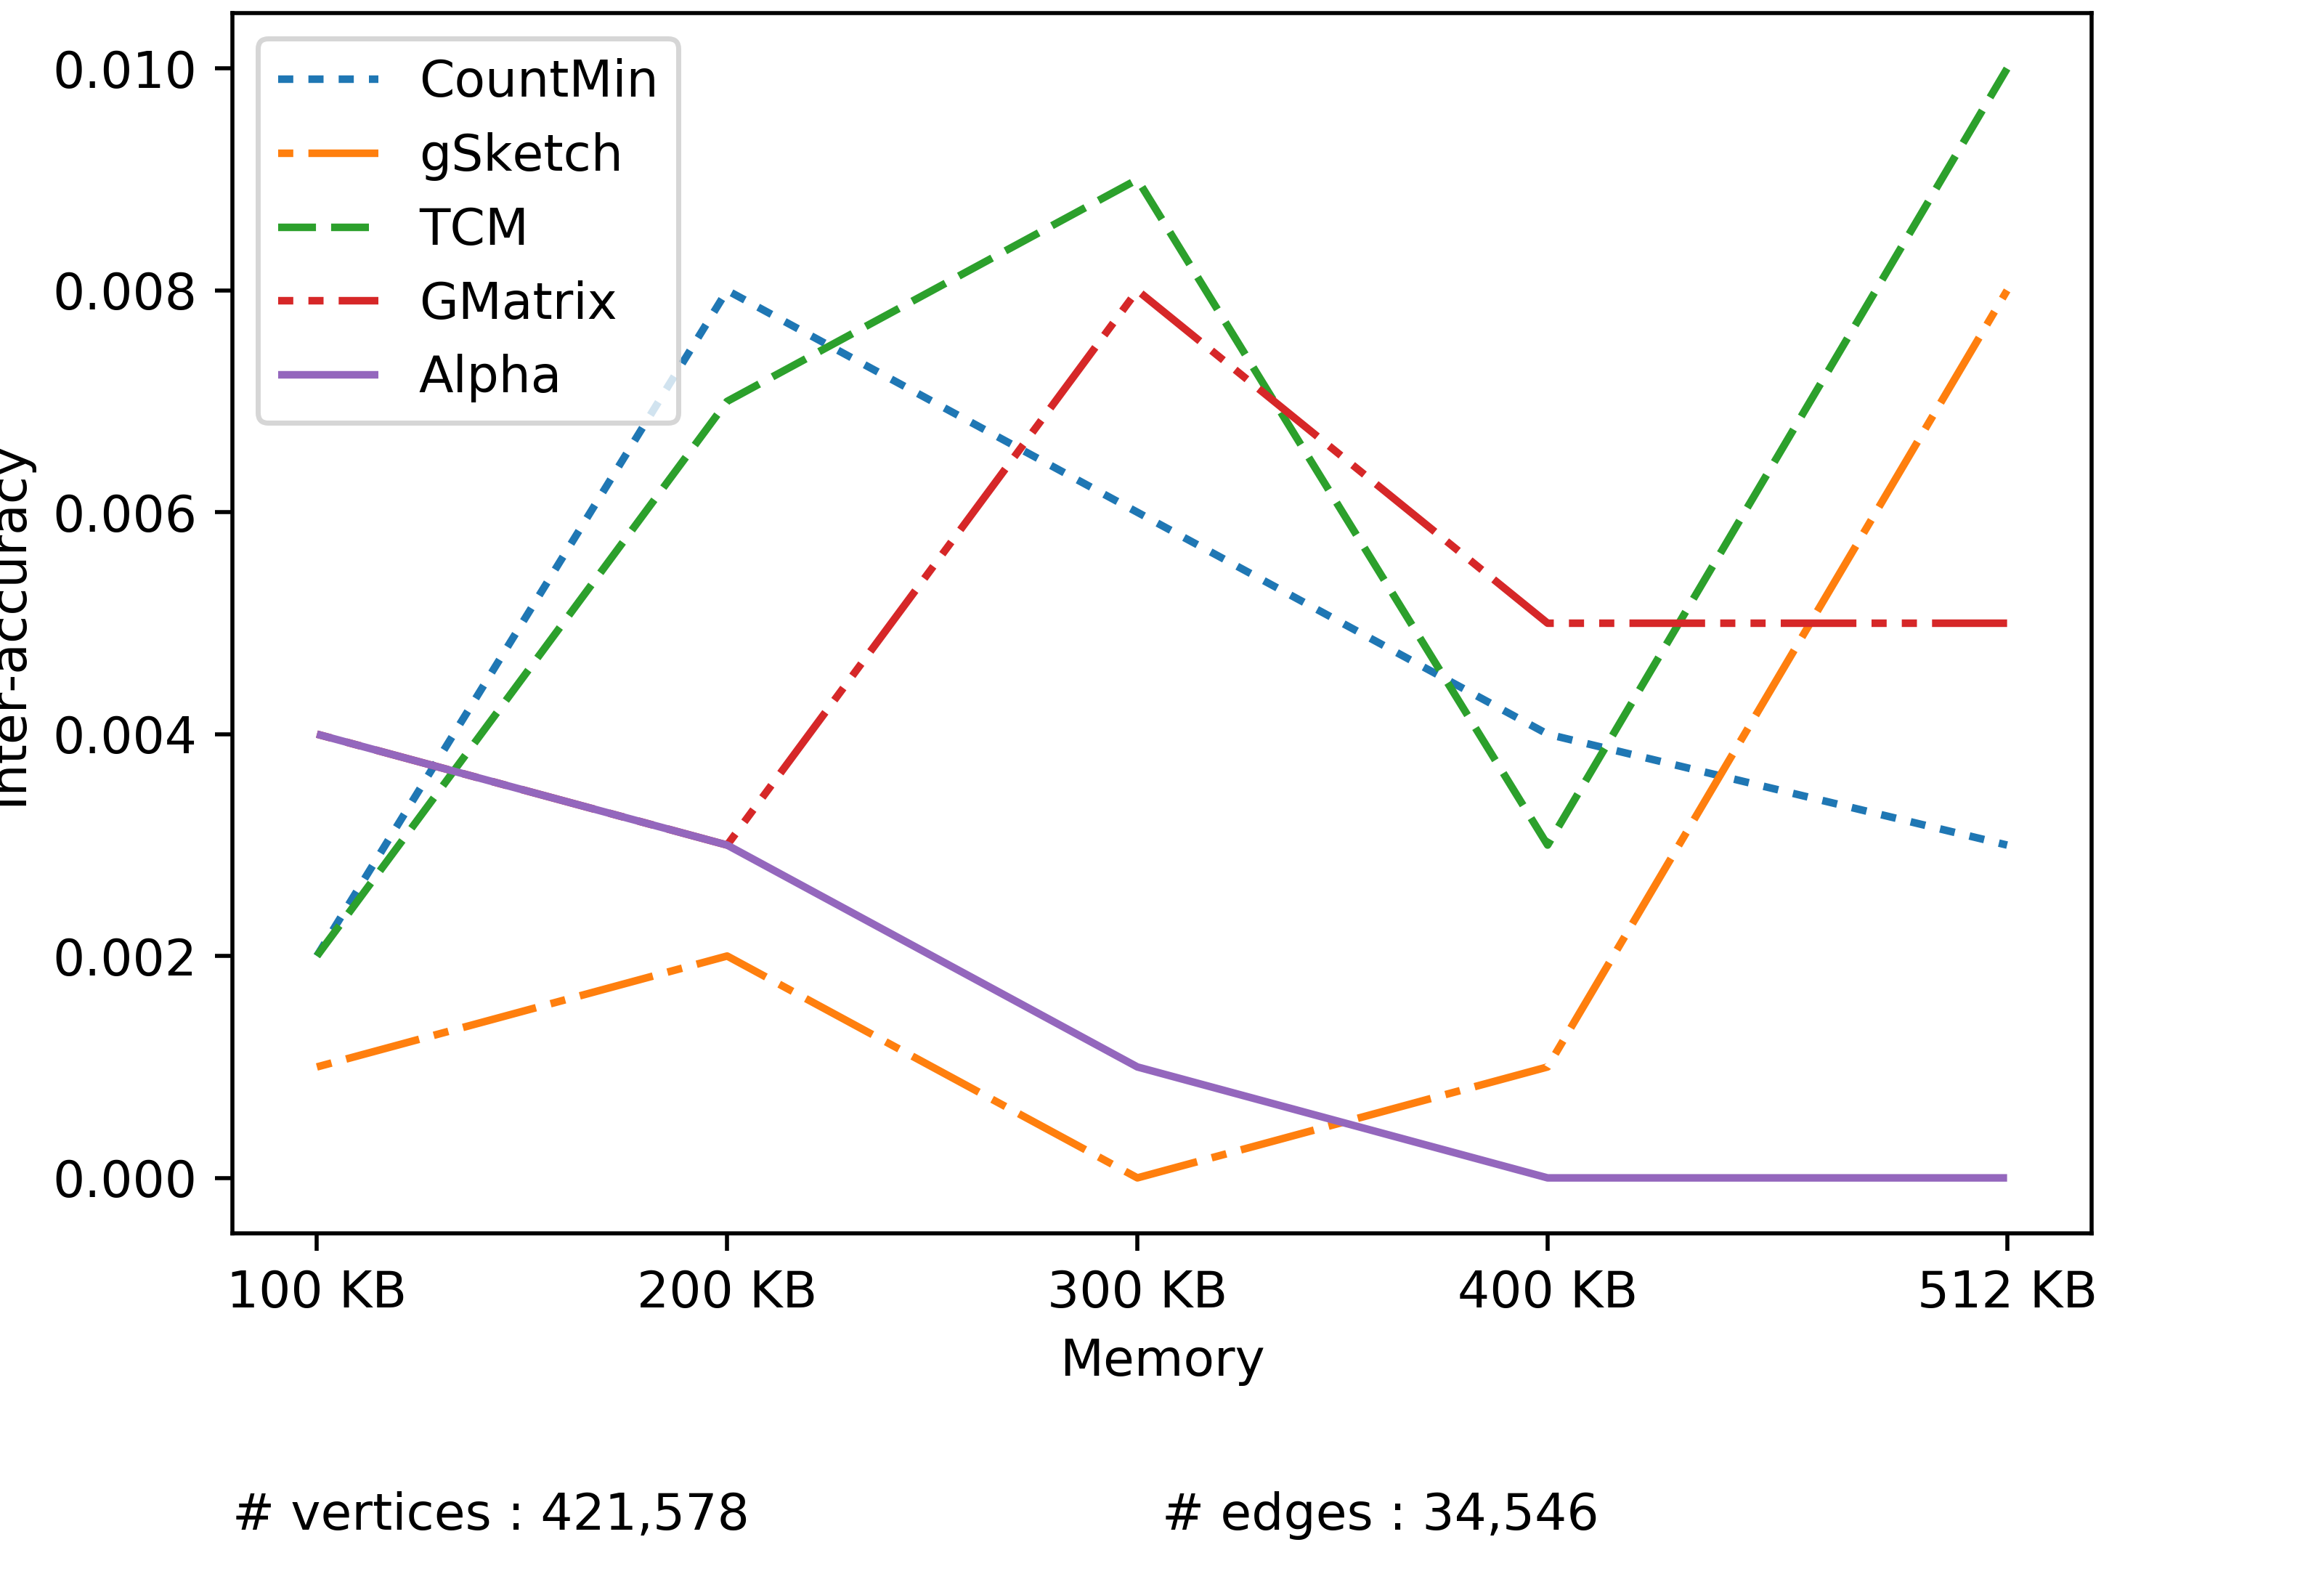
\includegraphics[width=0.85\textwidth]{results/he/cit-HepPh-he}
    \vspace{-0.5cm}
    \caption{Inter accuracy of heavy edges vs Memory for cit-HepPh dataset}
    \label{fig:cit-HepPh-he}
\end{figure}

\begin{figure}[H]
    \centering 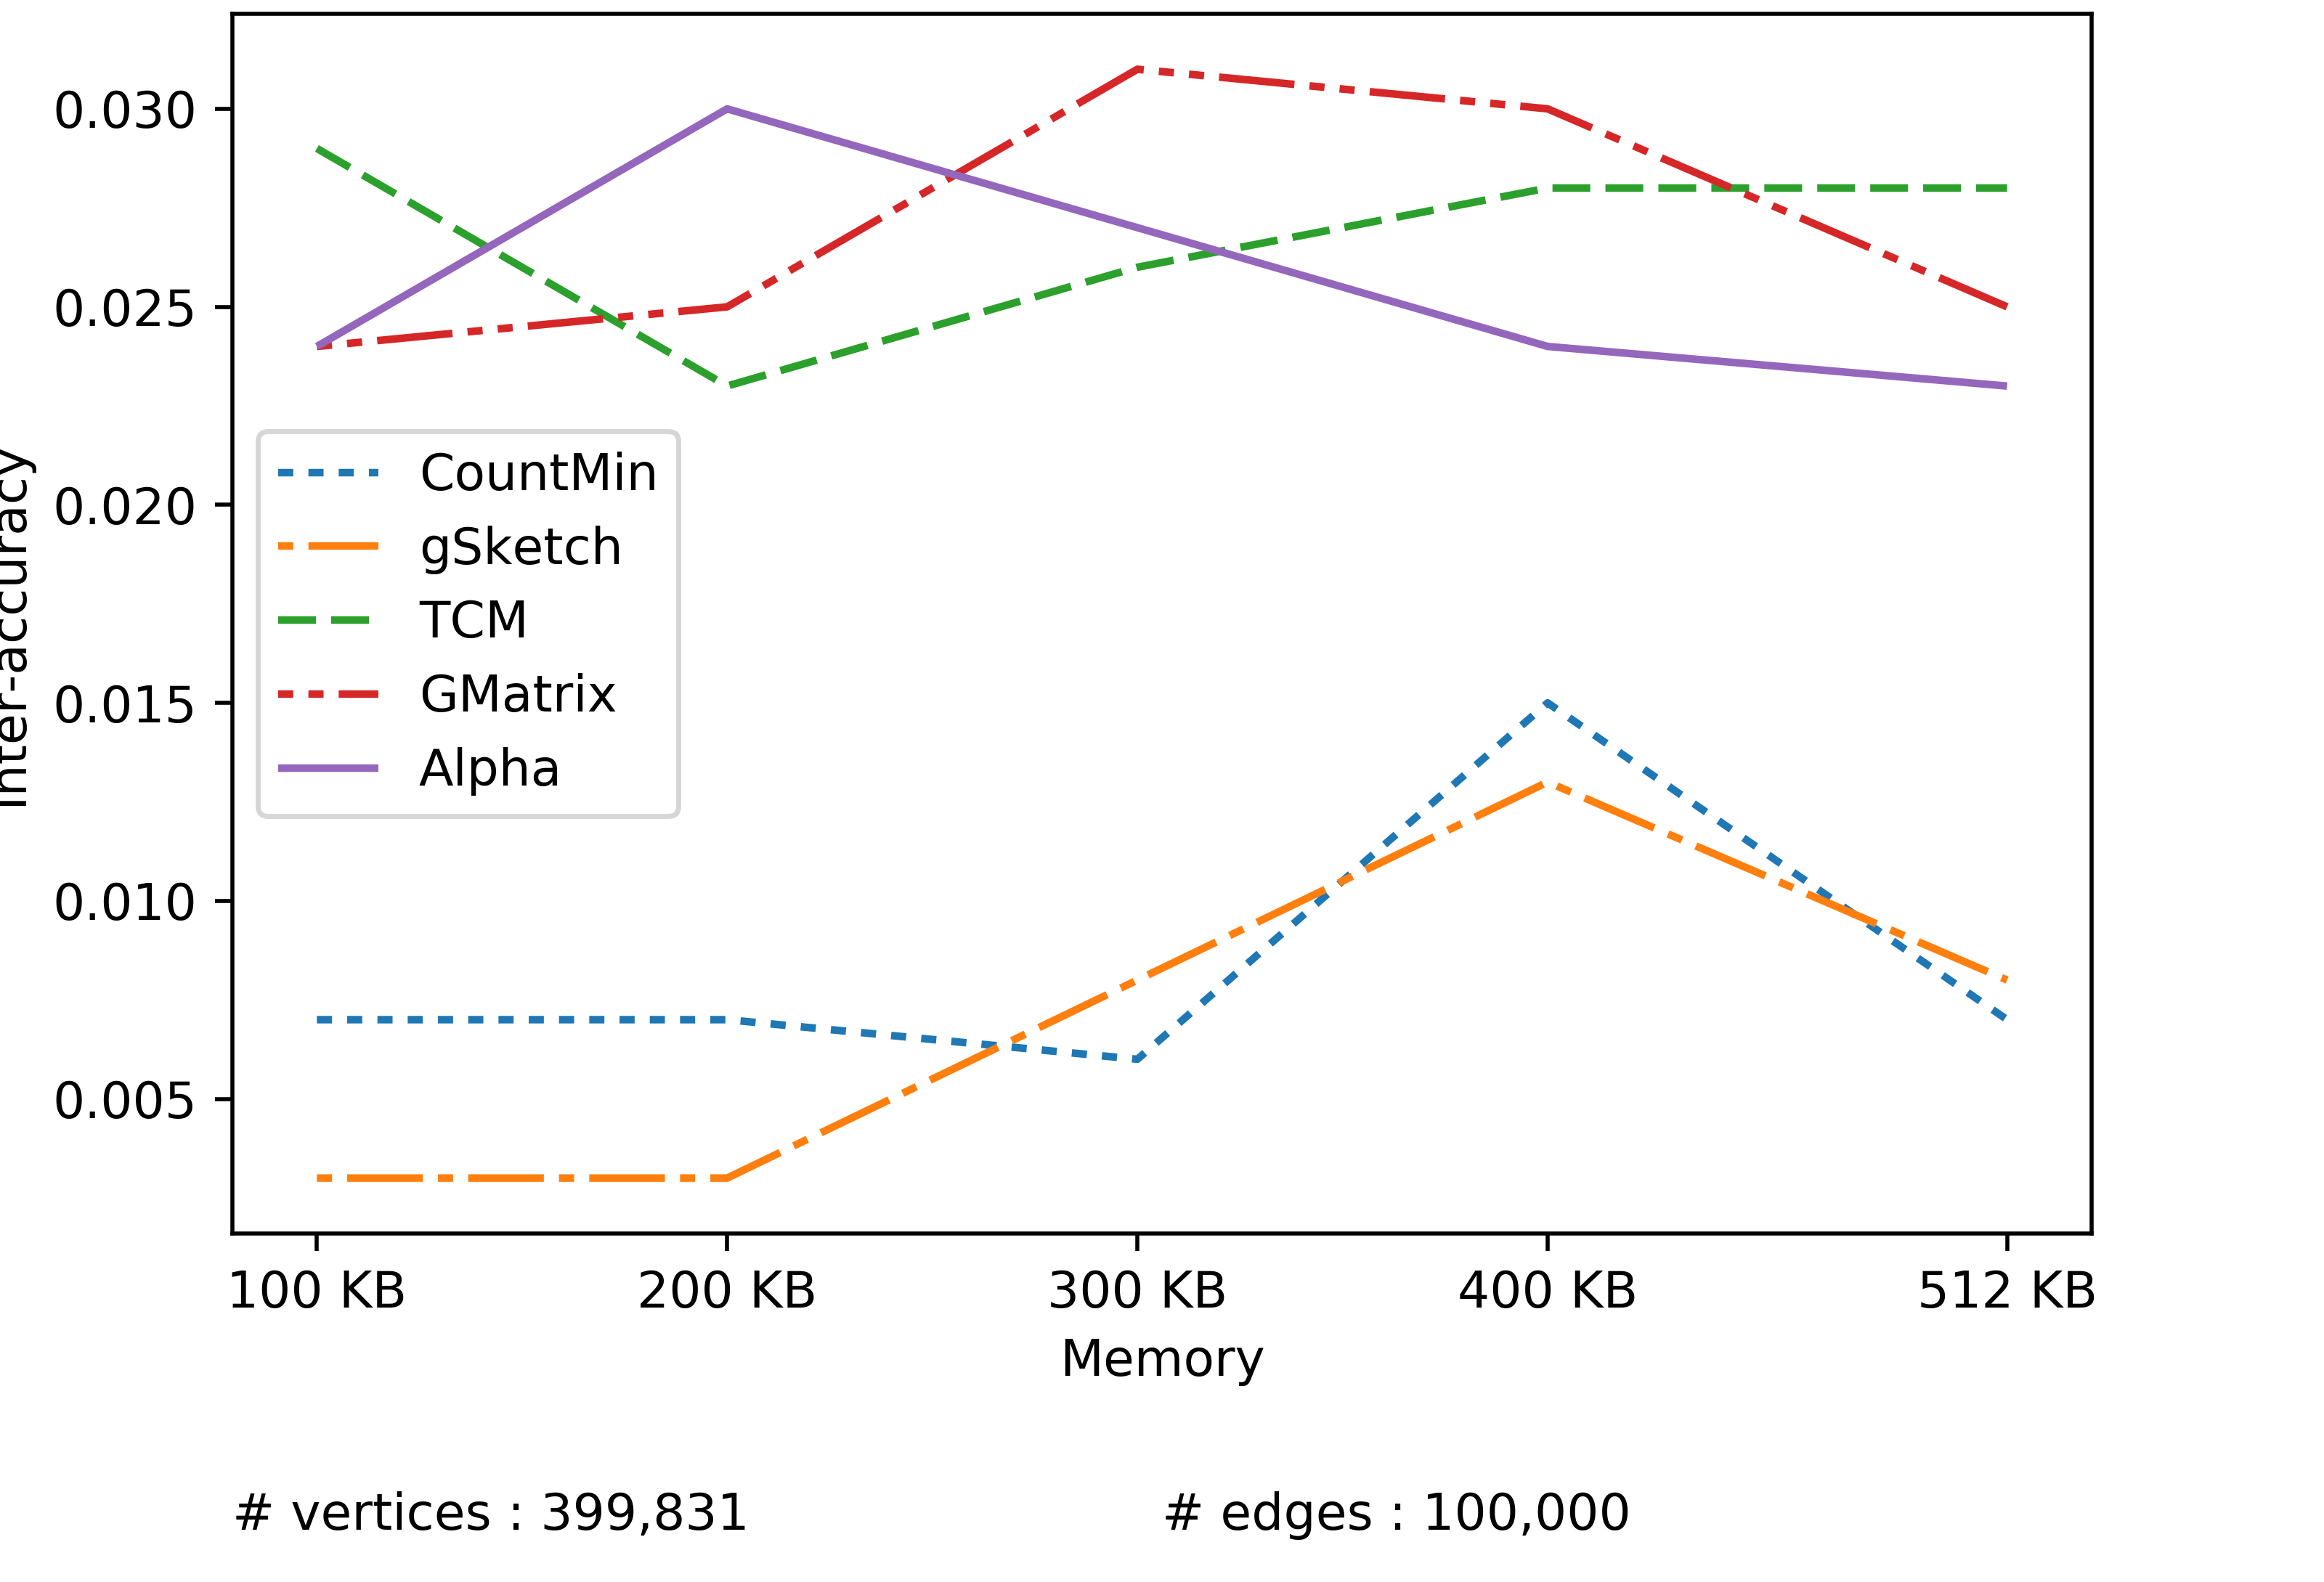
\includegraphics[width=0.85\textwidth]{results/he/gen-scale-free-he}
    \vspace{-0.5cm}
    \caption{Inter accuracy of heavy edges vs Memory for gen-scale-free dataset}
    \label{fig:gen-scale-free-he}
\end{figure}

\begin{figure}[H]
    \centering 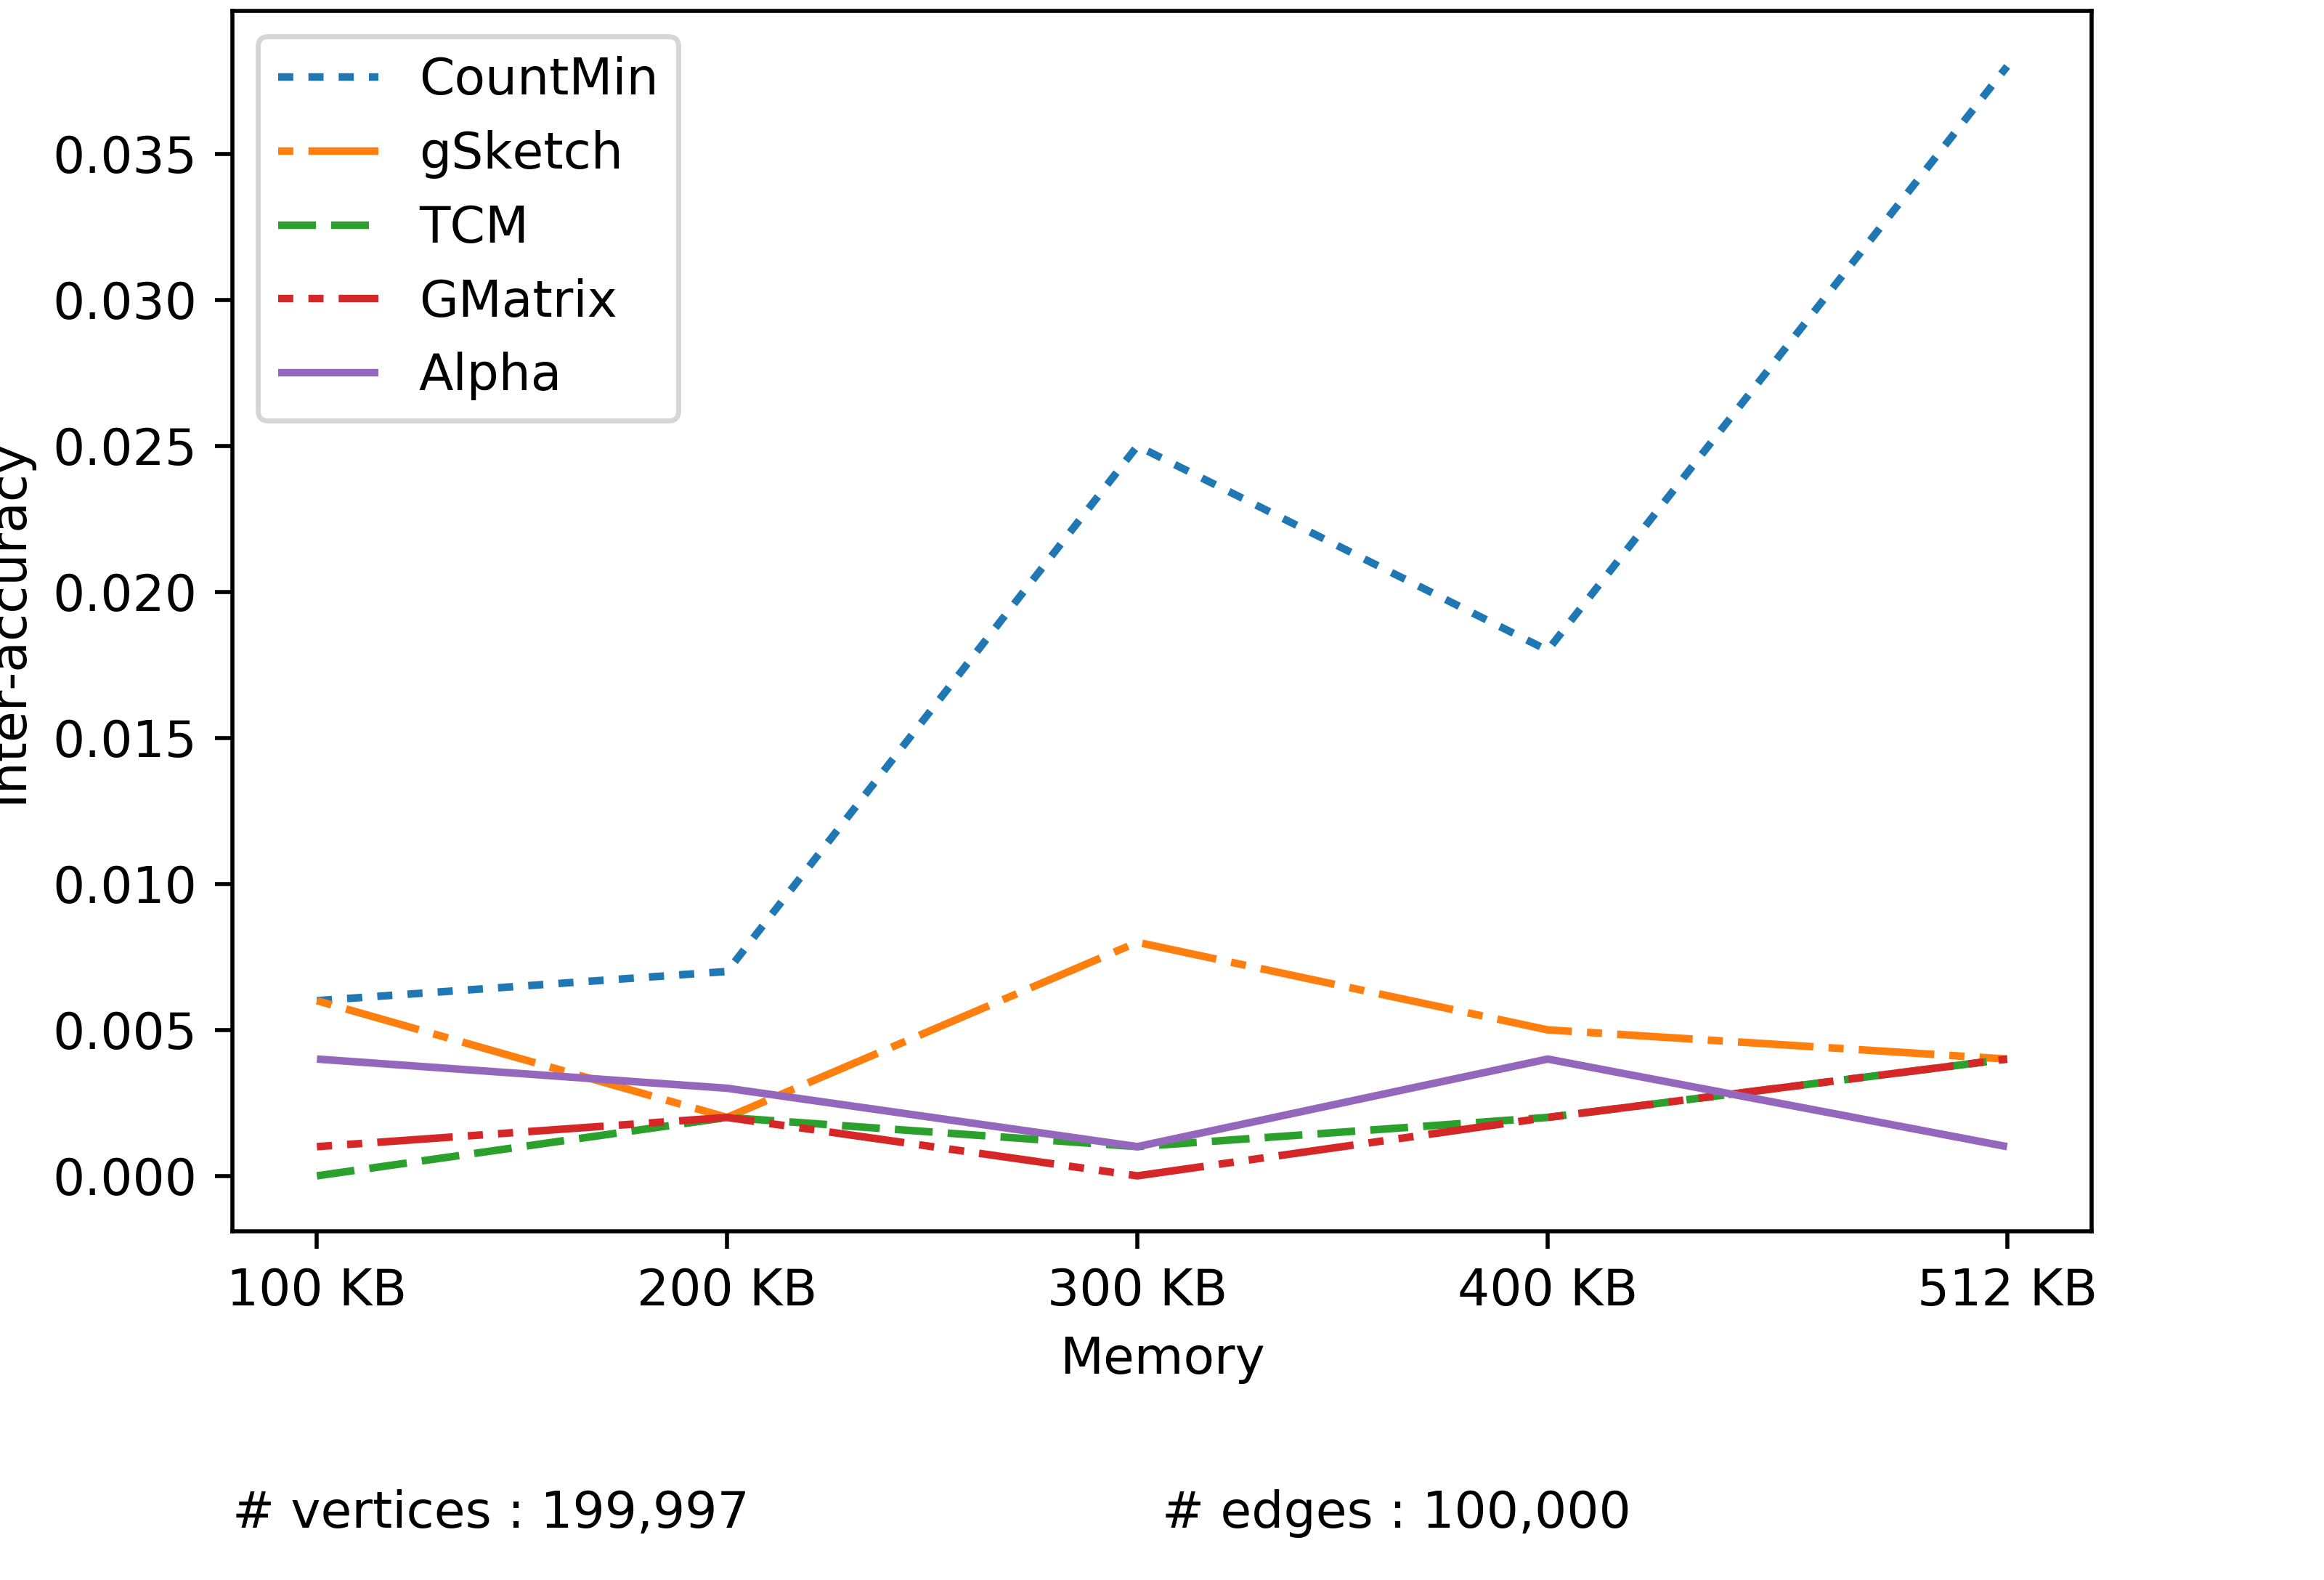
\includegraphics[width=0.85\textwidth]{results/he/gen-small-world-he}
    \vspace{-0.5cm}
    \caption{Inter accuracy of heavy edges vs Memory for gen-small-world dataset}
    \label{fig:gen-small-world-he}
\end{figure}

\subsection*{Observations and inferences}

\paragraph{}
Both the partitioned sketches, gSketch and Alpha has shown comparably low inter accuracies for top-k heavy edge queries for the datasets, unicorn-wget in \autoref{fig:unicorn-wget-he}, email-EuAll in \autoref{fig:email-EuAll-he} and cit-HepPh in \autoref{fig:cit-HepPh-he}. Thus we can infer that the partitioning of the sketches has negatively affected the performance of heavy edge queries.

\paragraph{}
The accuracy of Alpha is relatively better in the generated gen-scale-free and gen-small-world datasets for some sketch sizes, which strictly follow the power law distribution properties.

\paragraph{}
The accuracy of the CountMin sketch with respect to heavy edge queries have suffered in comparison to the results of the heavy node queries in the \autoref{section:heavy_nodes}. However CountMin sketch can still be proposed as a reliable sketch in answering heavy edge queries for graph streams in general.
\section{Degree distribution}

\subsection*{Purpose}

\paragraph{}
To compare the vertex degree distribution of the original graph stream and the graph depicted by the summarized sketch.

\subsection*{Results}

\begin{figure}[H]
    \centering 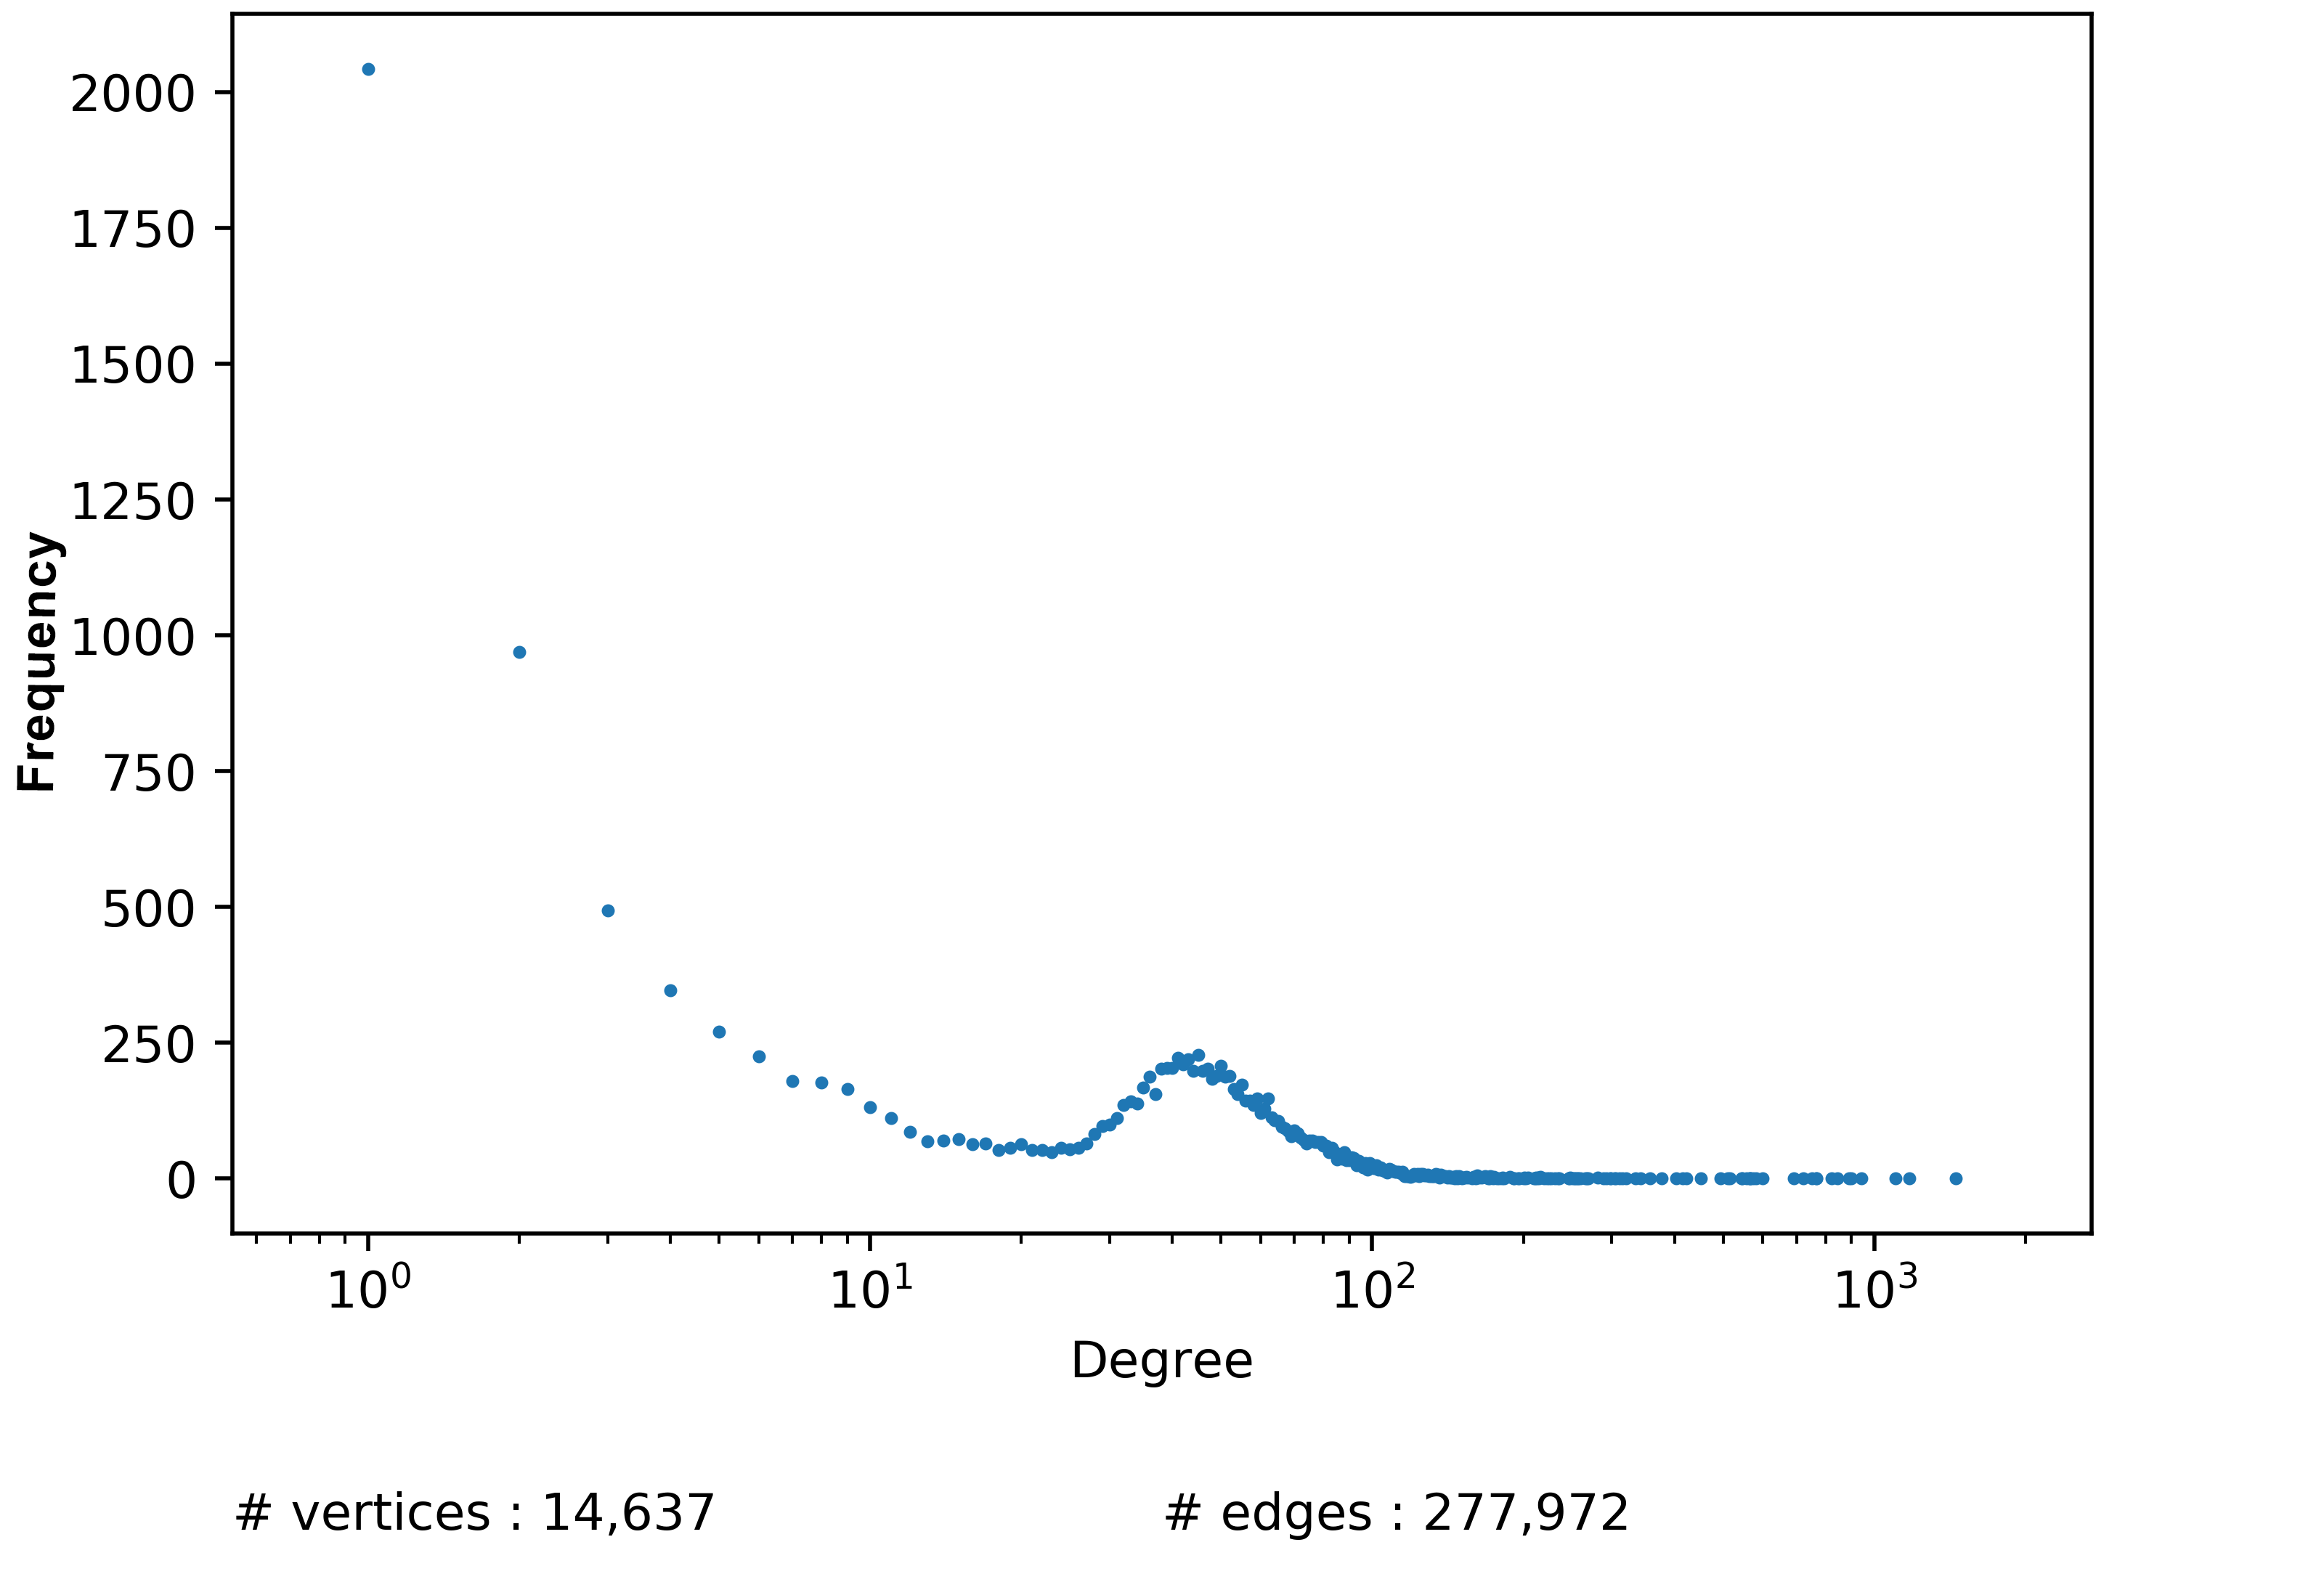
\includegraphics[width=0.85\textwidth]{results/dd/unicorn-wget-dd-fullgraph}
    \vspace{-0.5cm}
    \caption{Degree distribution of FullGraph for unicorn-wget dataset}
    \label{fig:unicorn-wget-dd-fullgraph}
\end{figure}

\begin{figure}[H]
    \centering 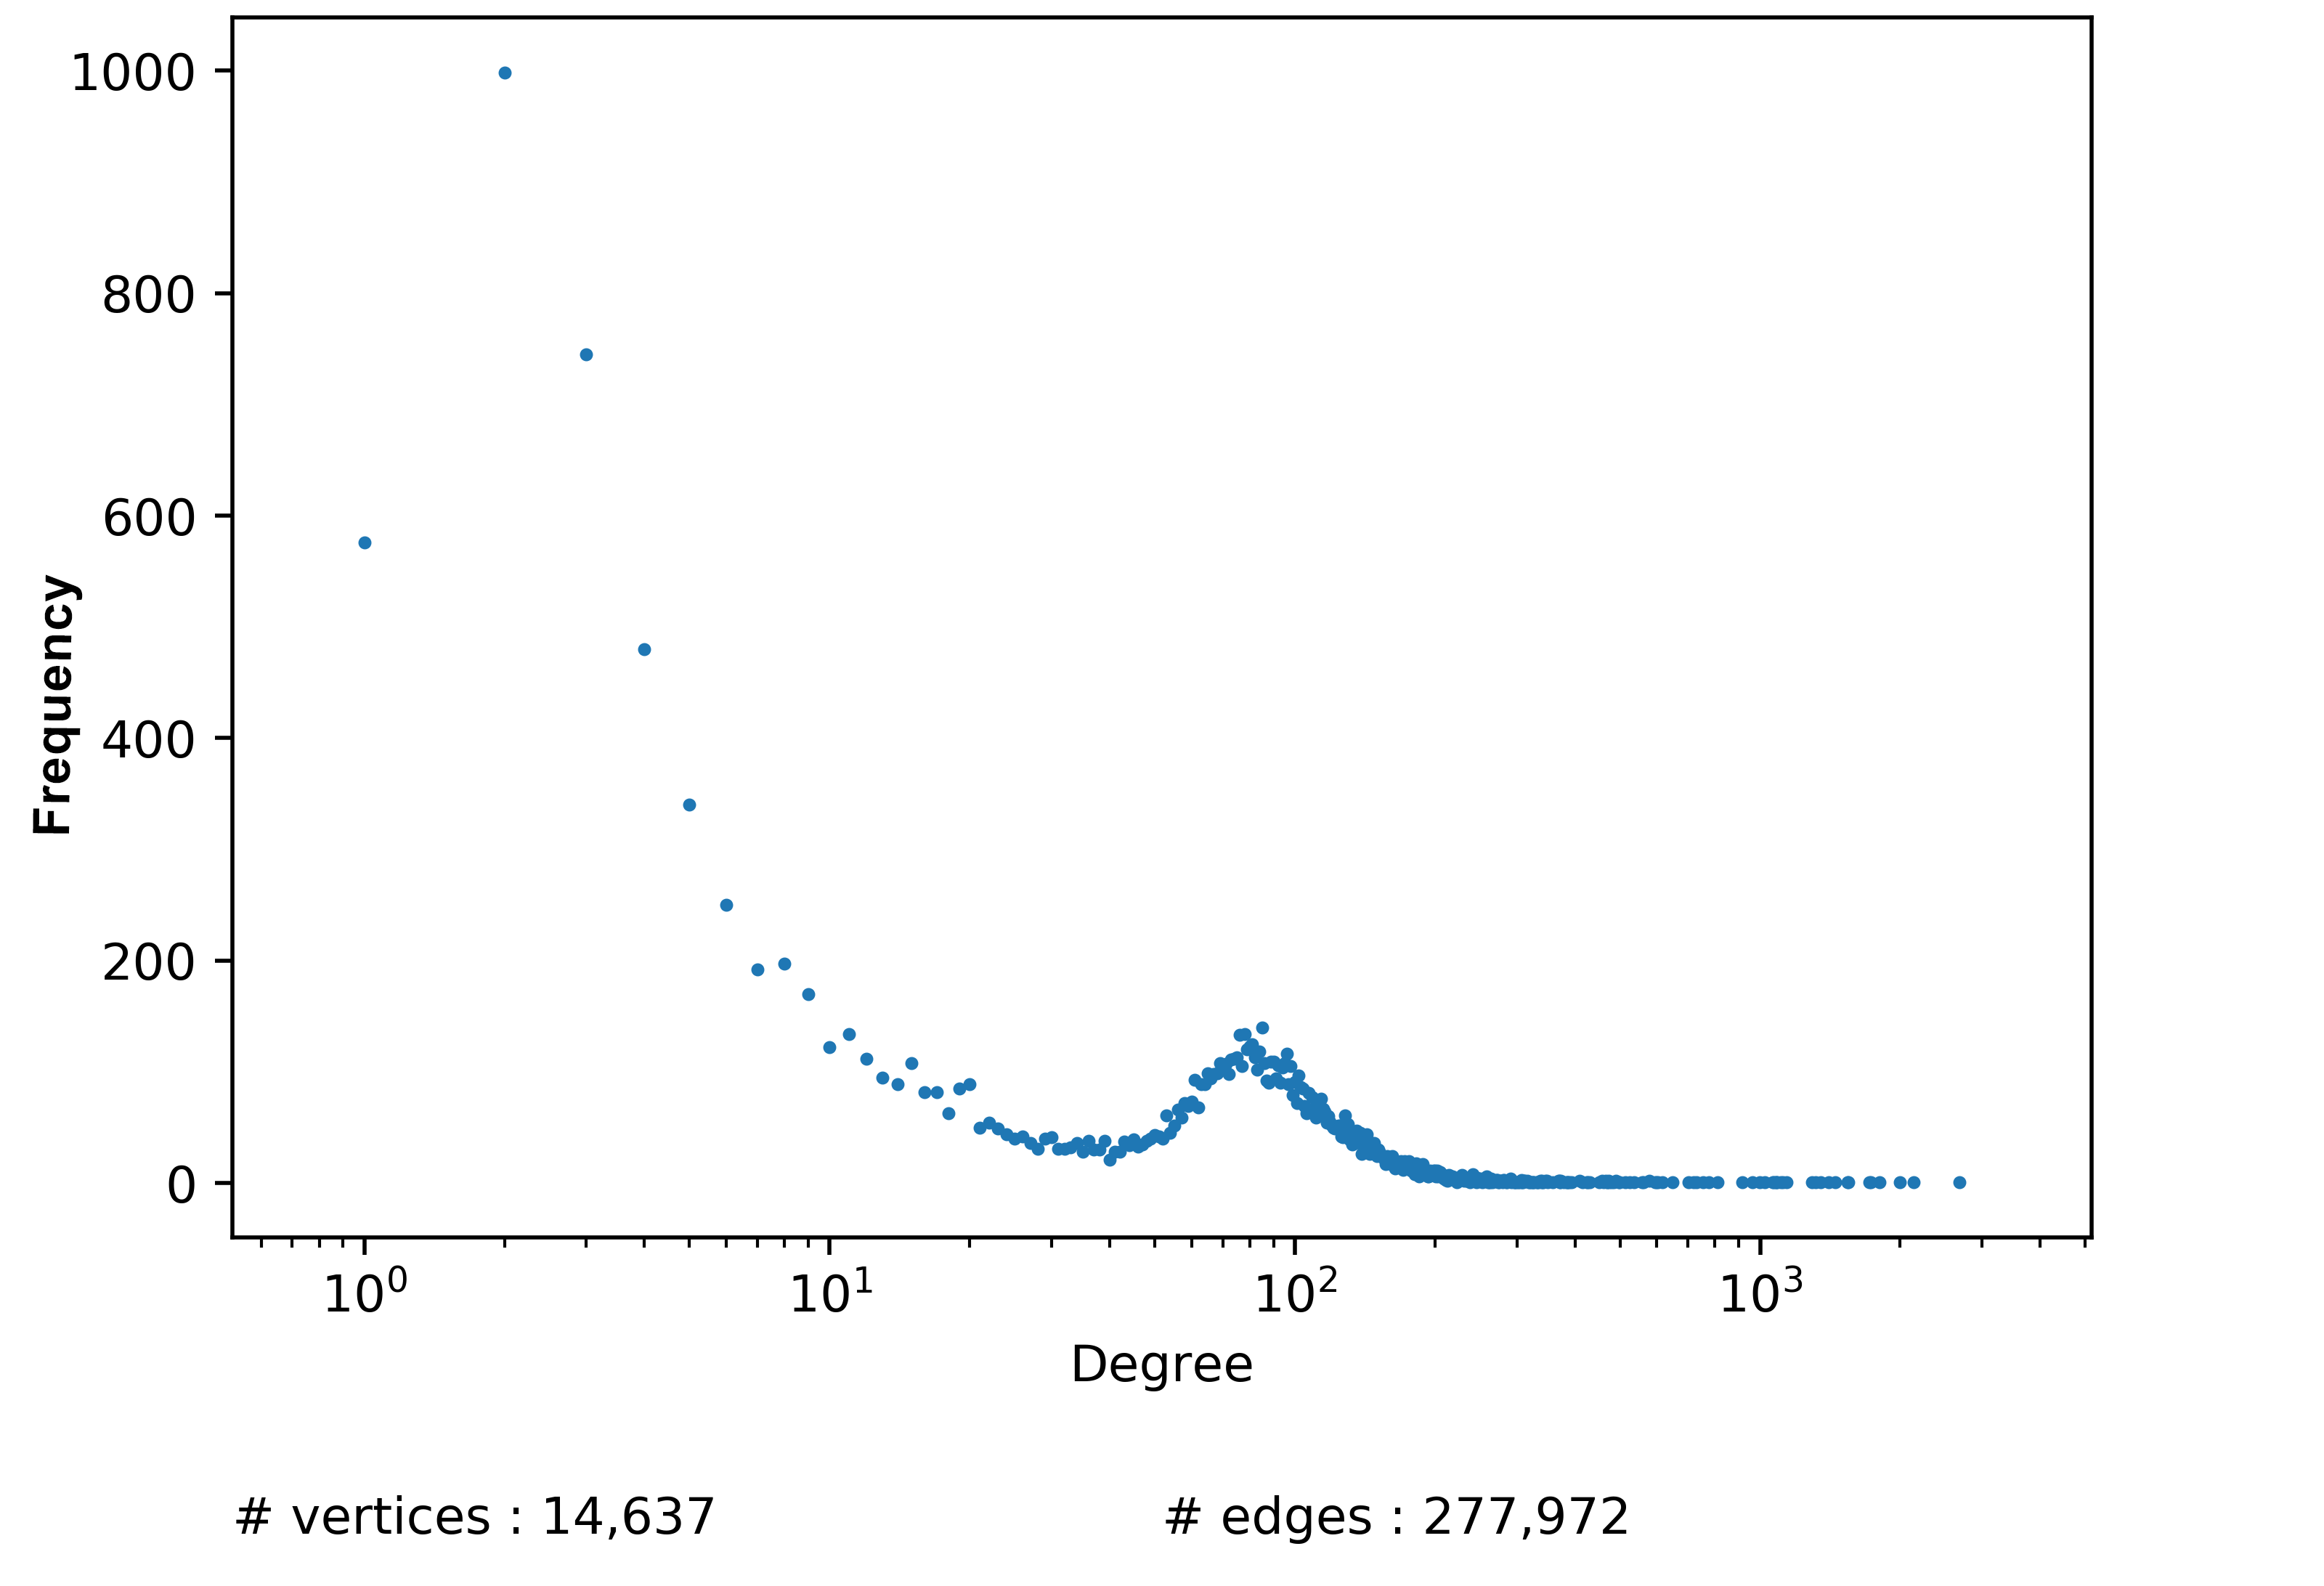
\includegraphics[width=0.85\textwidth]{results/dd/unicorn-wget-dd-countmin_1024}
    \vspace{-0.5cm}
    \caption{Degree distribution of CountMin for unicorn-wget dataset}
    \label{fig:unicorn-wget-dd-countmin_1024}
\end{figure}

\begin{figure}[H]
    \centering 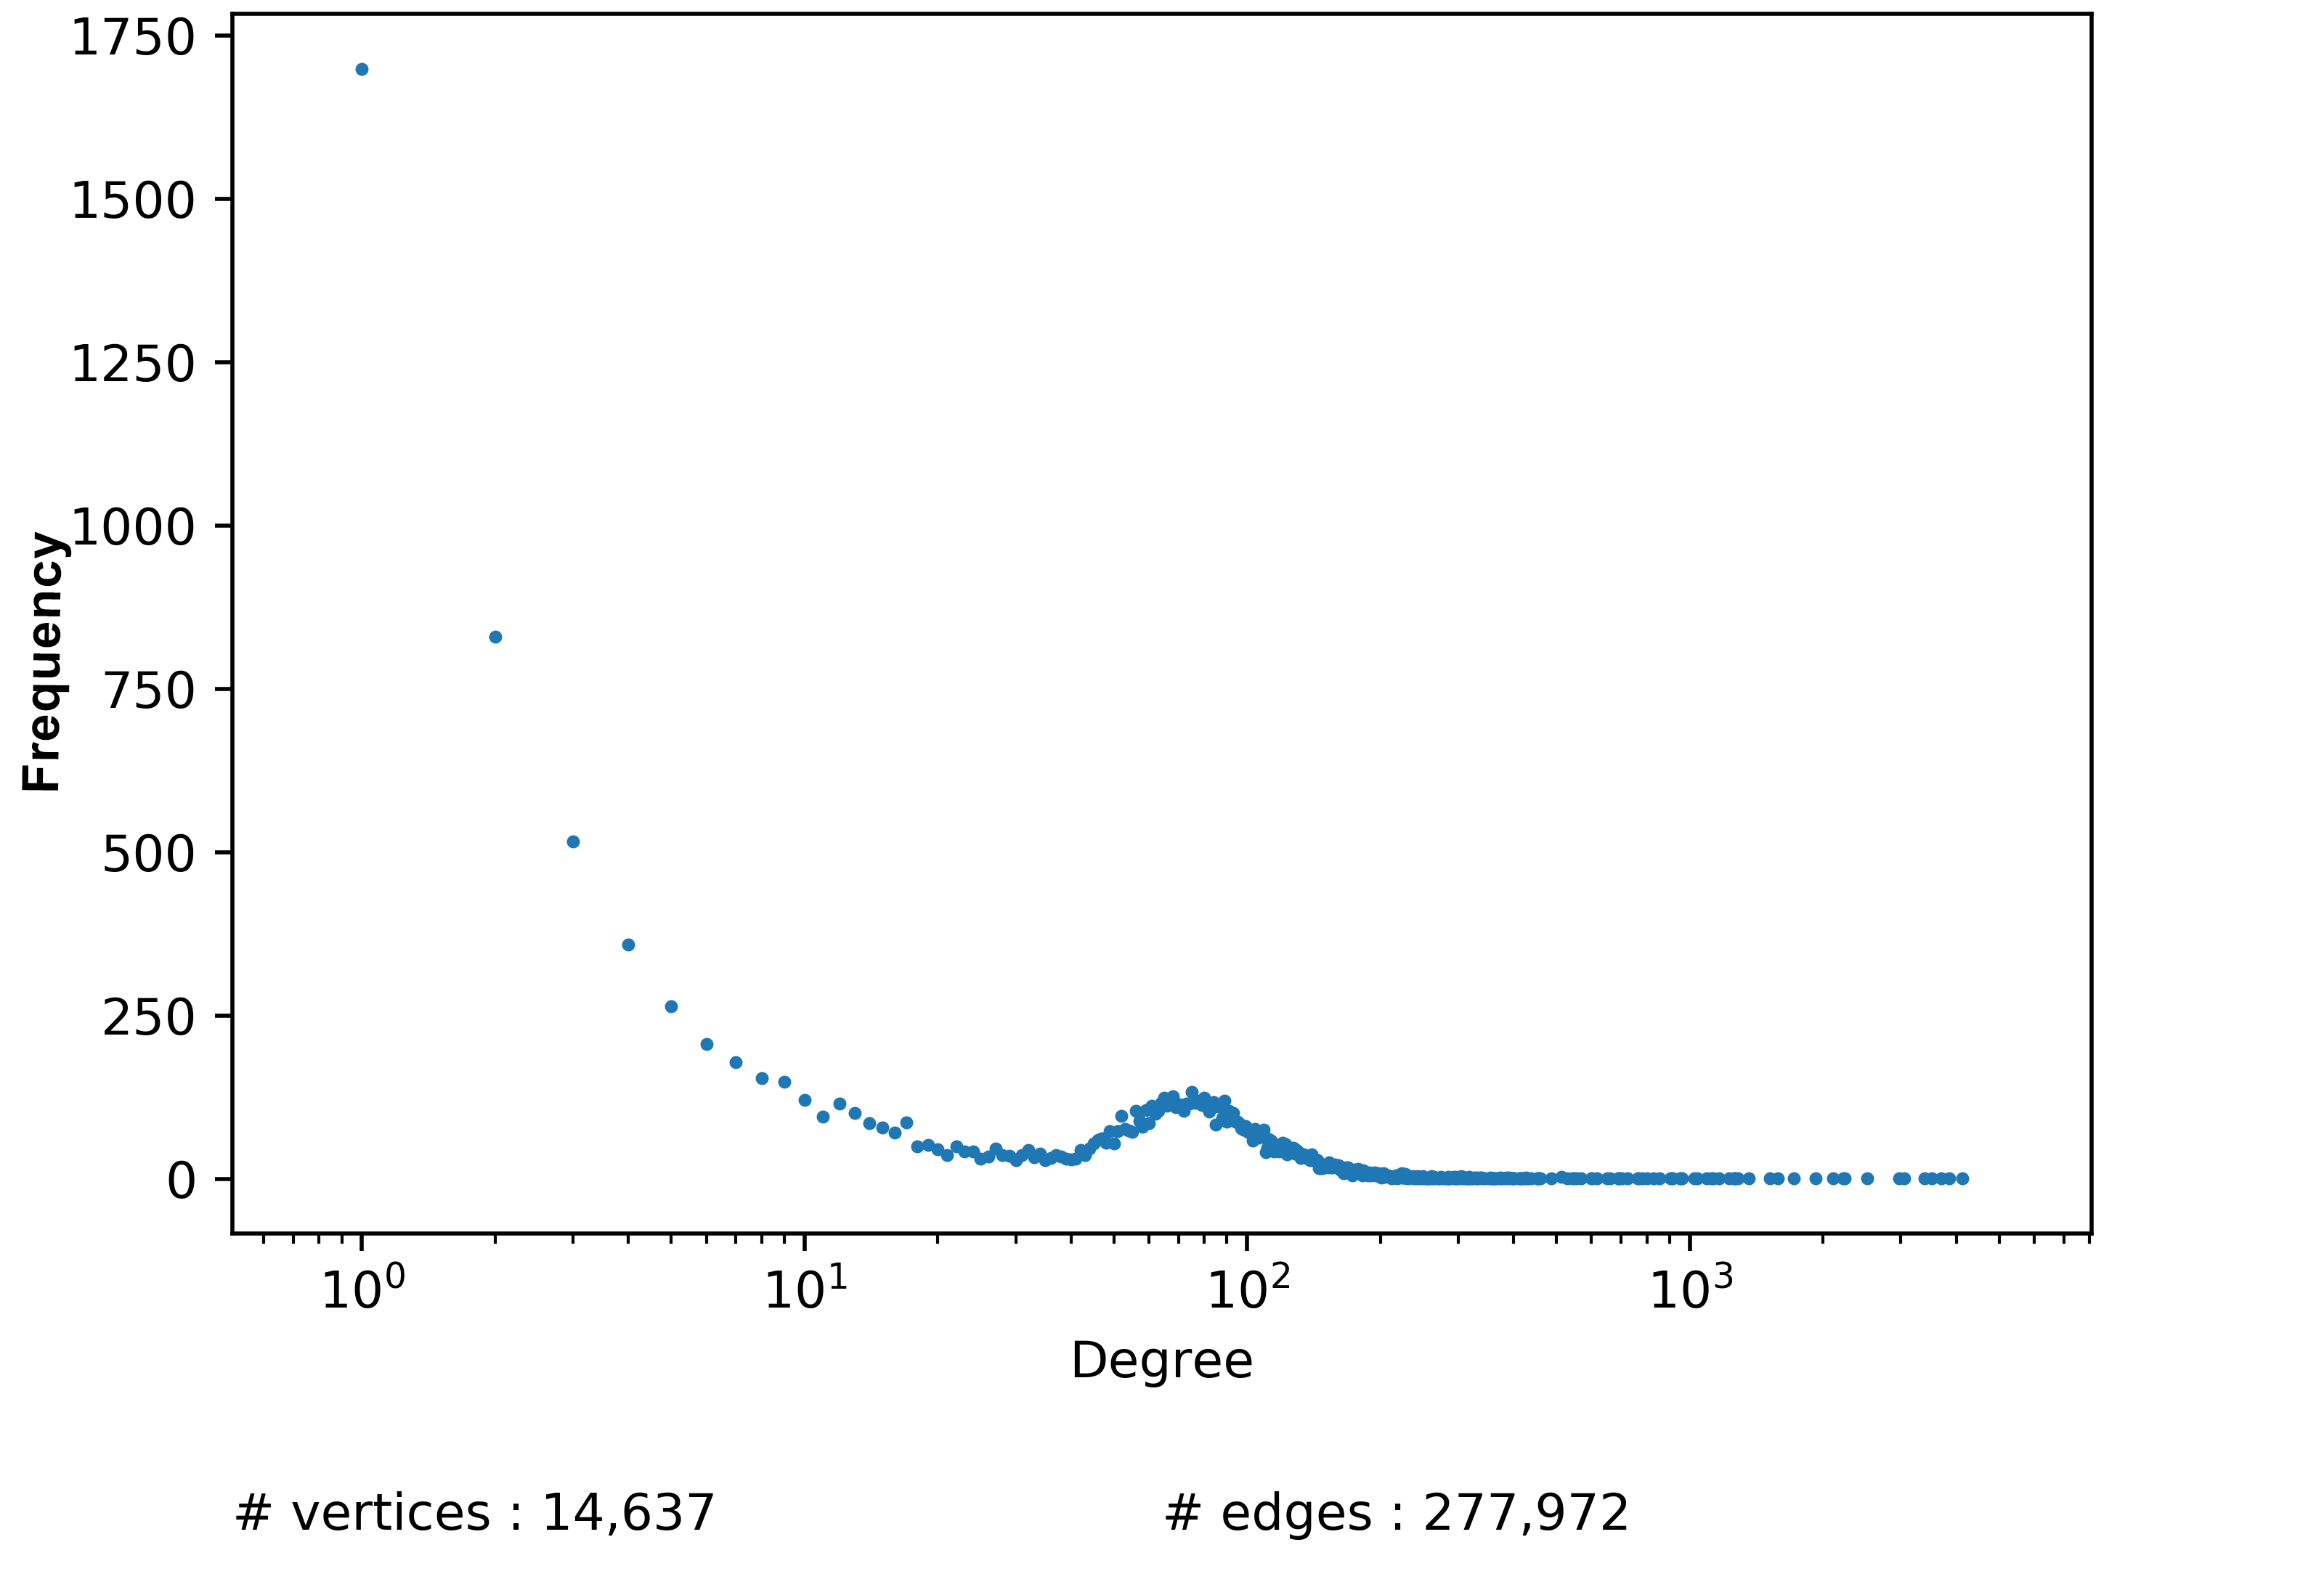
\includegraphics[width=0.85\textwidth]{results/dd/unicorn-wget-dd-gsketch_1024}
    \vspace{-0.5cm}
    \caption{Degree distribution of gSketch for unicorn-wget dataset}
    \label{fig:unicorn-wget-dd-gsketch_1024}
\end{figure}

\begin{figure}[H]
    \centering 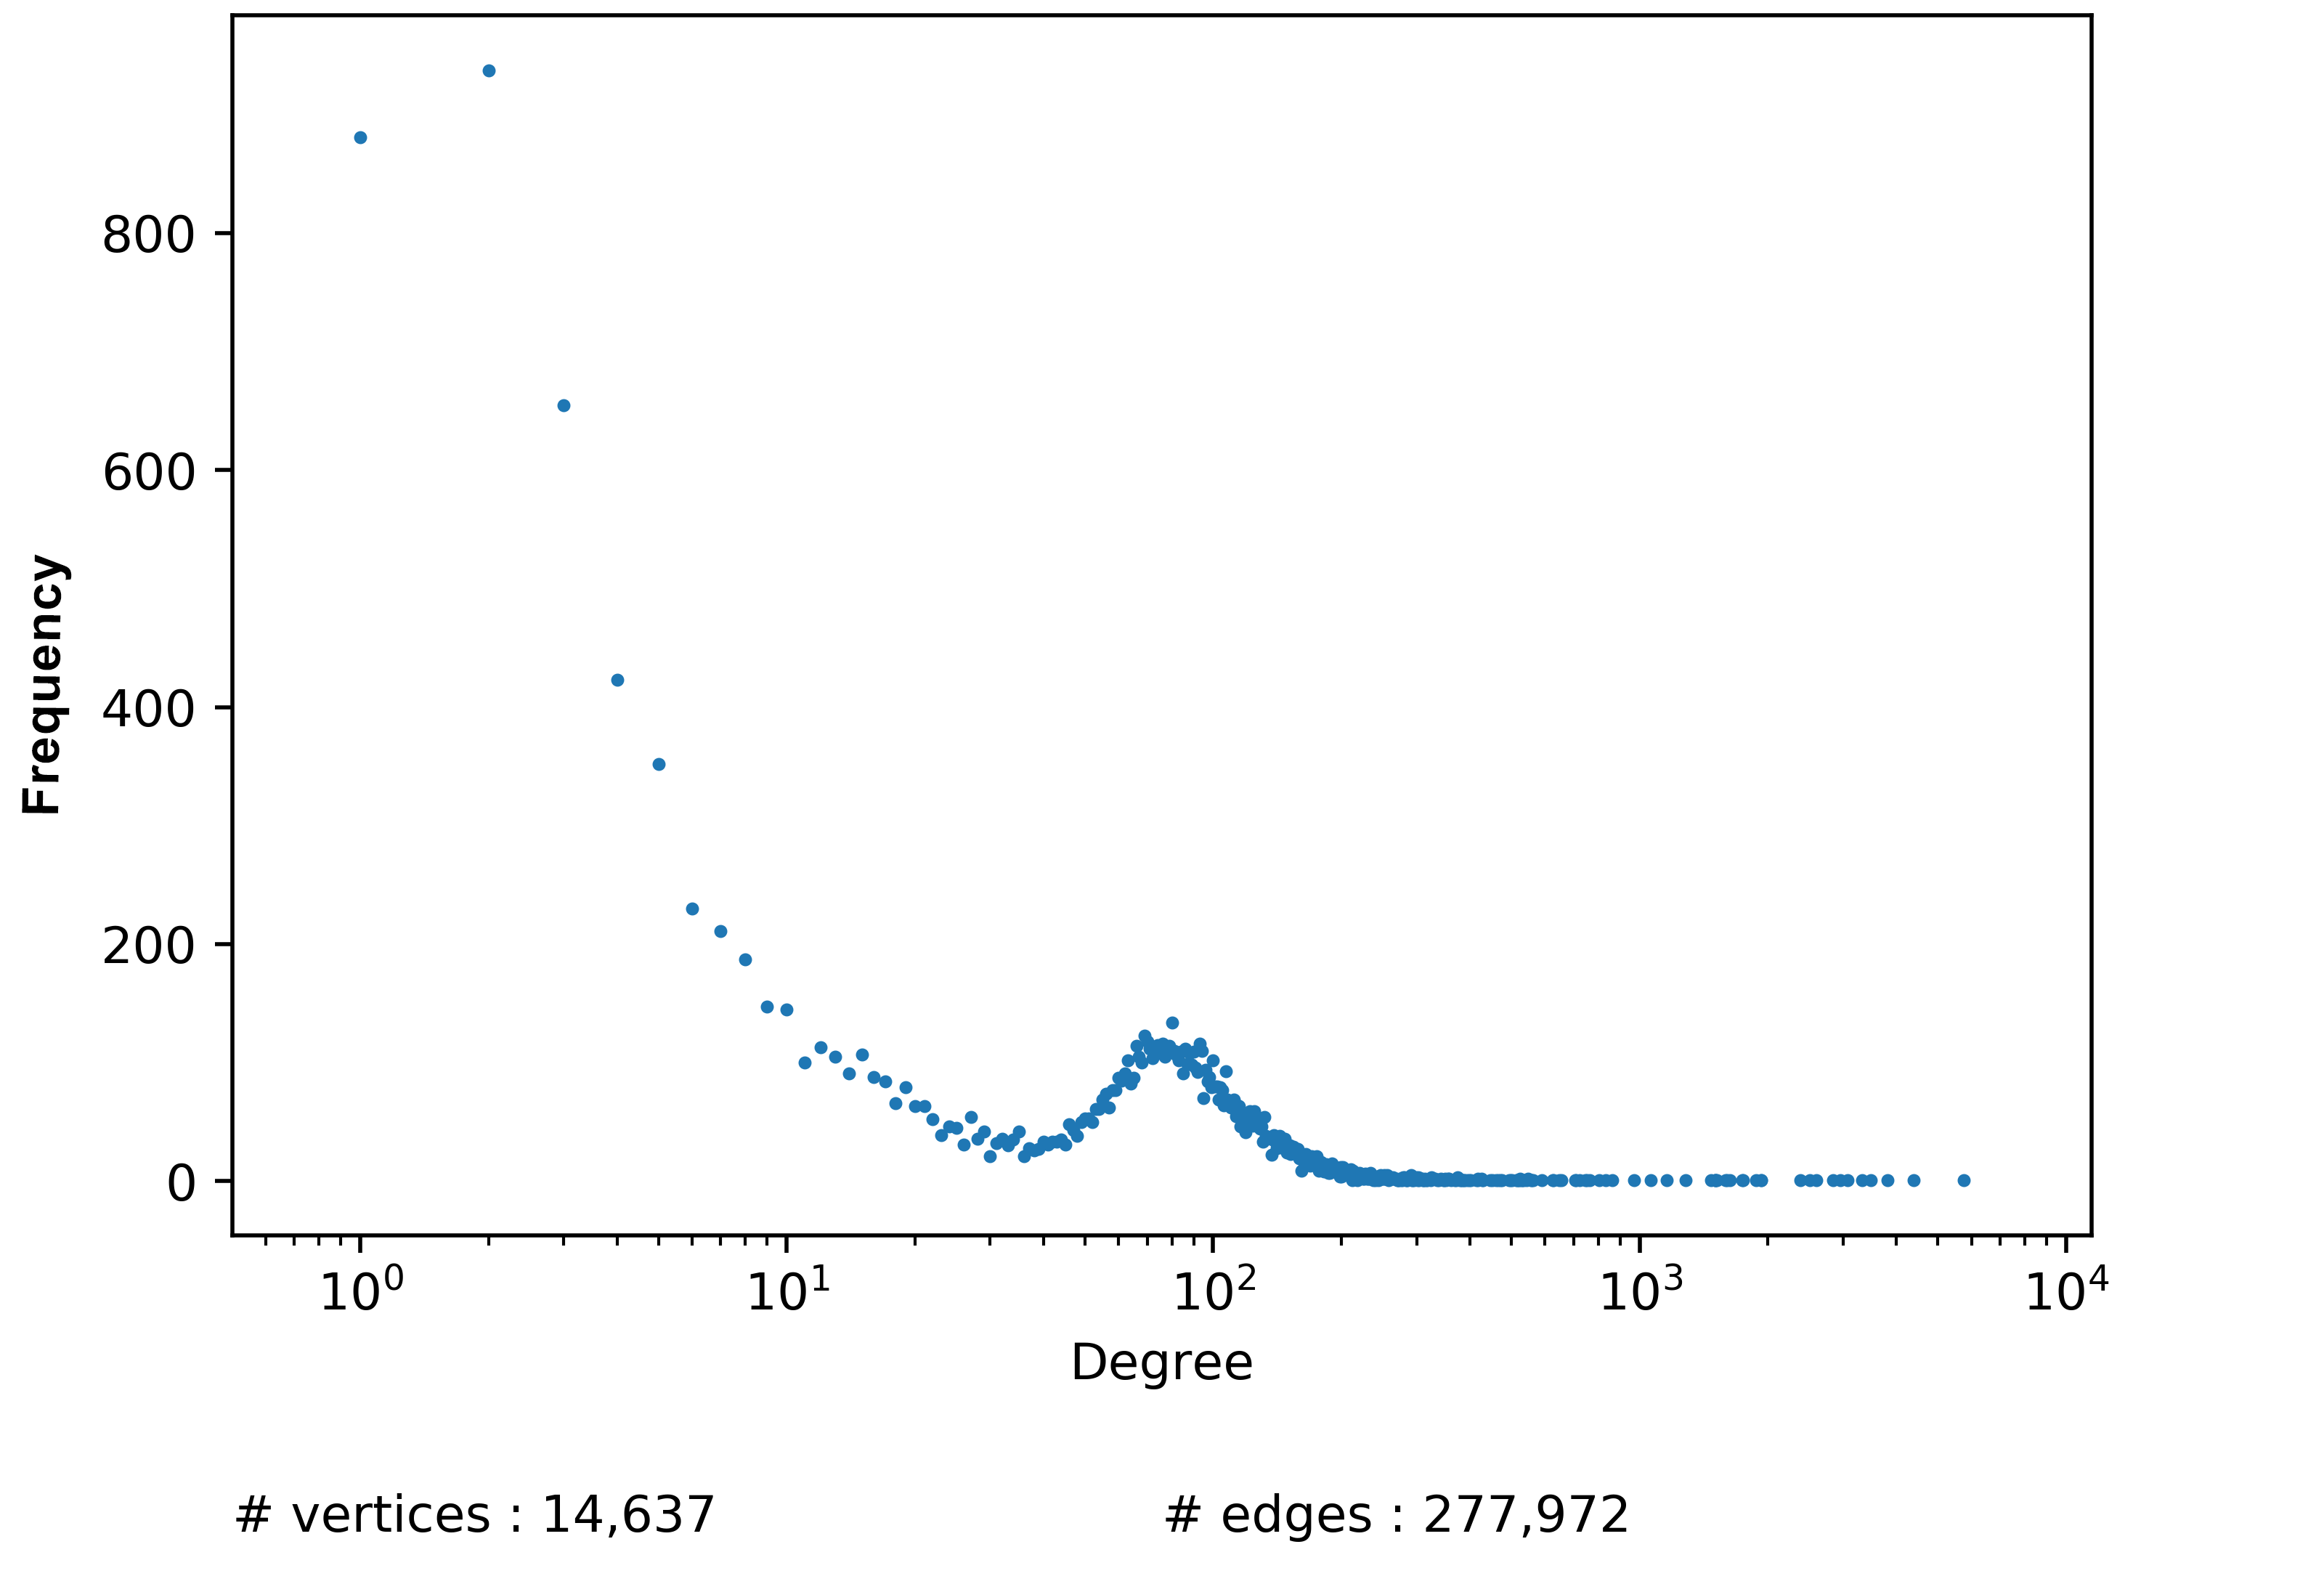
\includegraphics[width=0.85\textwidth]{results/dd/unicorn-wget-dd-tcm_1024}
    \vspace{-0.5cm}
    \caption{Degree distribution of TCM for unicorn-wget dataset}
    \label{fig:unicorn-wget-dd-tcm_1024}
\end{figure}

\begin{figure}[H]
    \centering 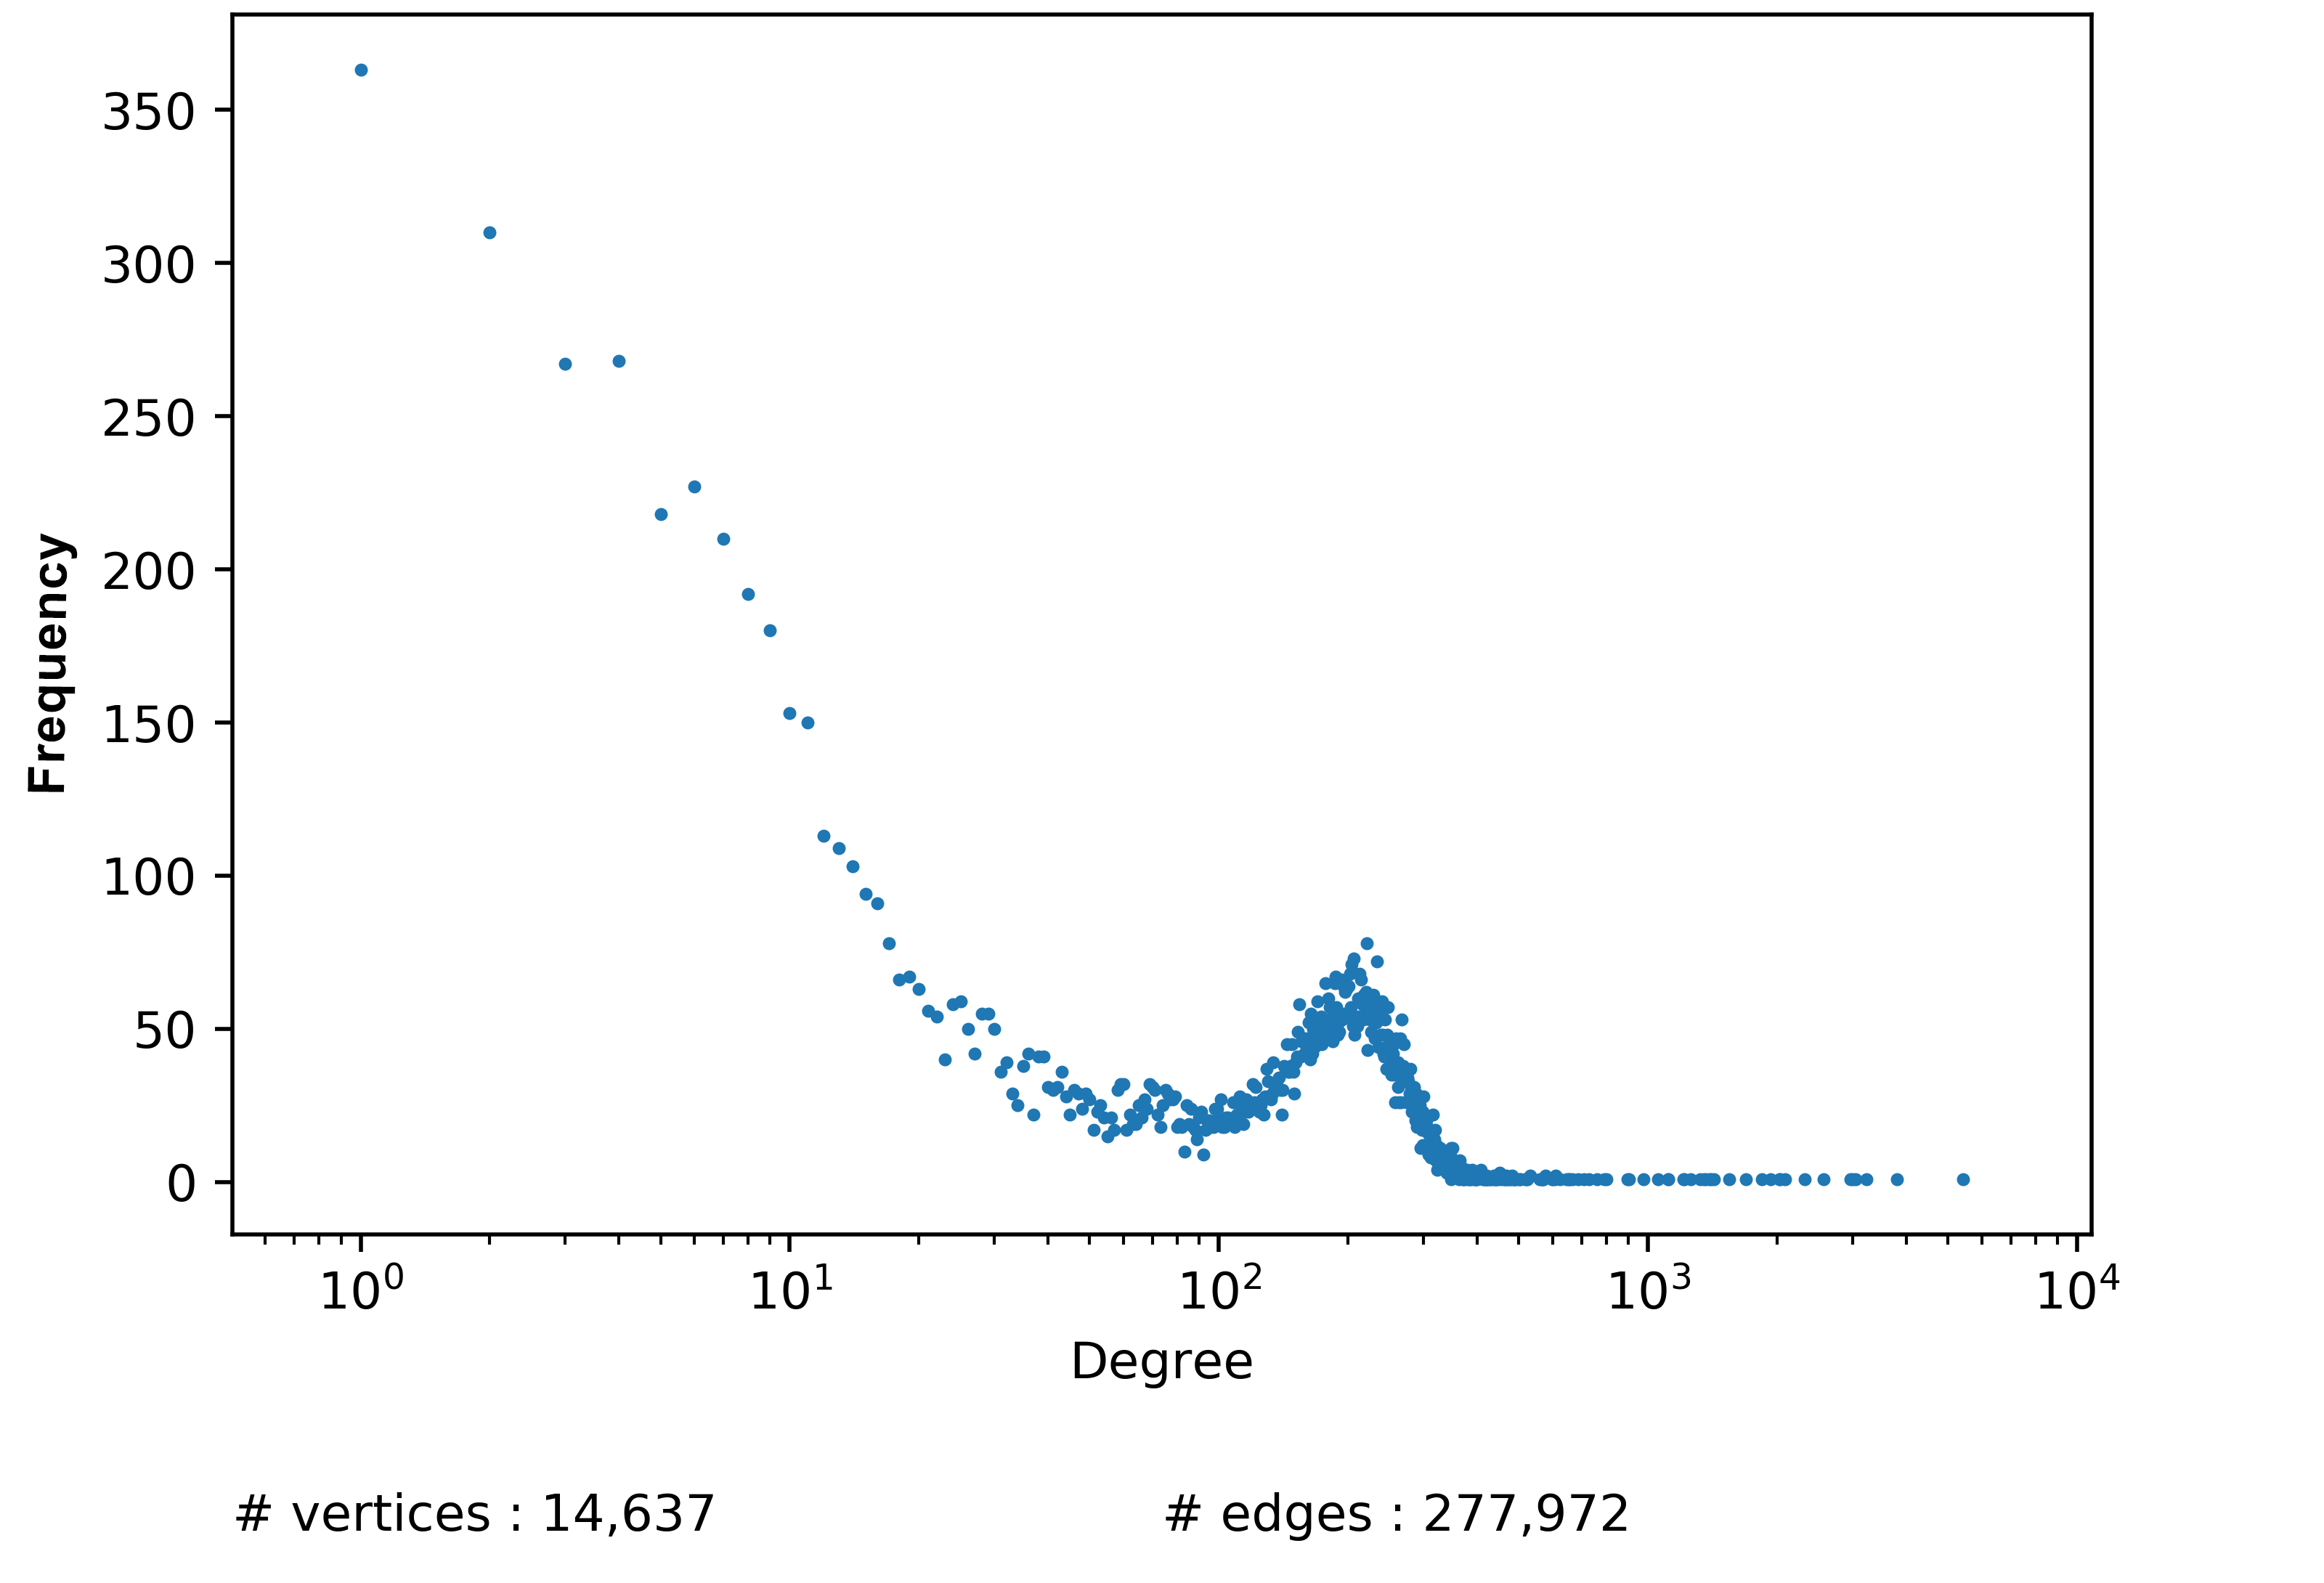
\includegraphics[width=0.85\textwidth]{results/dd/unicorn-wget-dd-gmatrix_1024}
    \vspace{-0.5cm}
    \caption{Degree distribution of GMatrix for unicorn-wget dataset}
    \label{fig:unicorn-wget-dd-gmatrix_1024}
\end{figure}

\begin{figure}[H]
    \centering 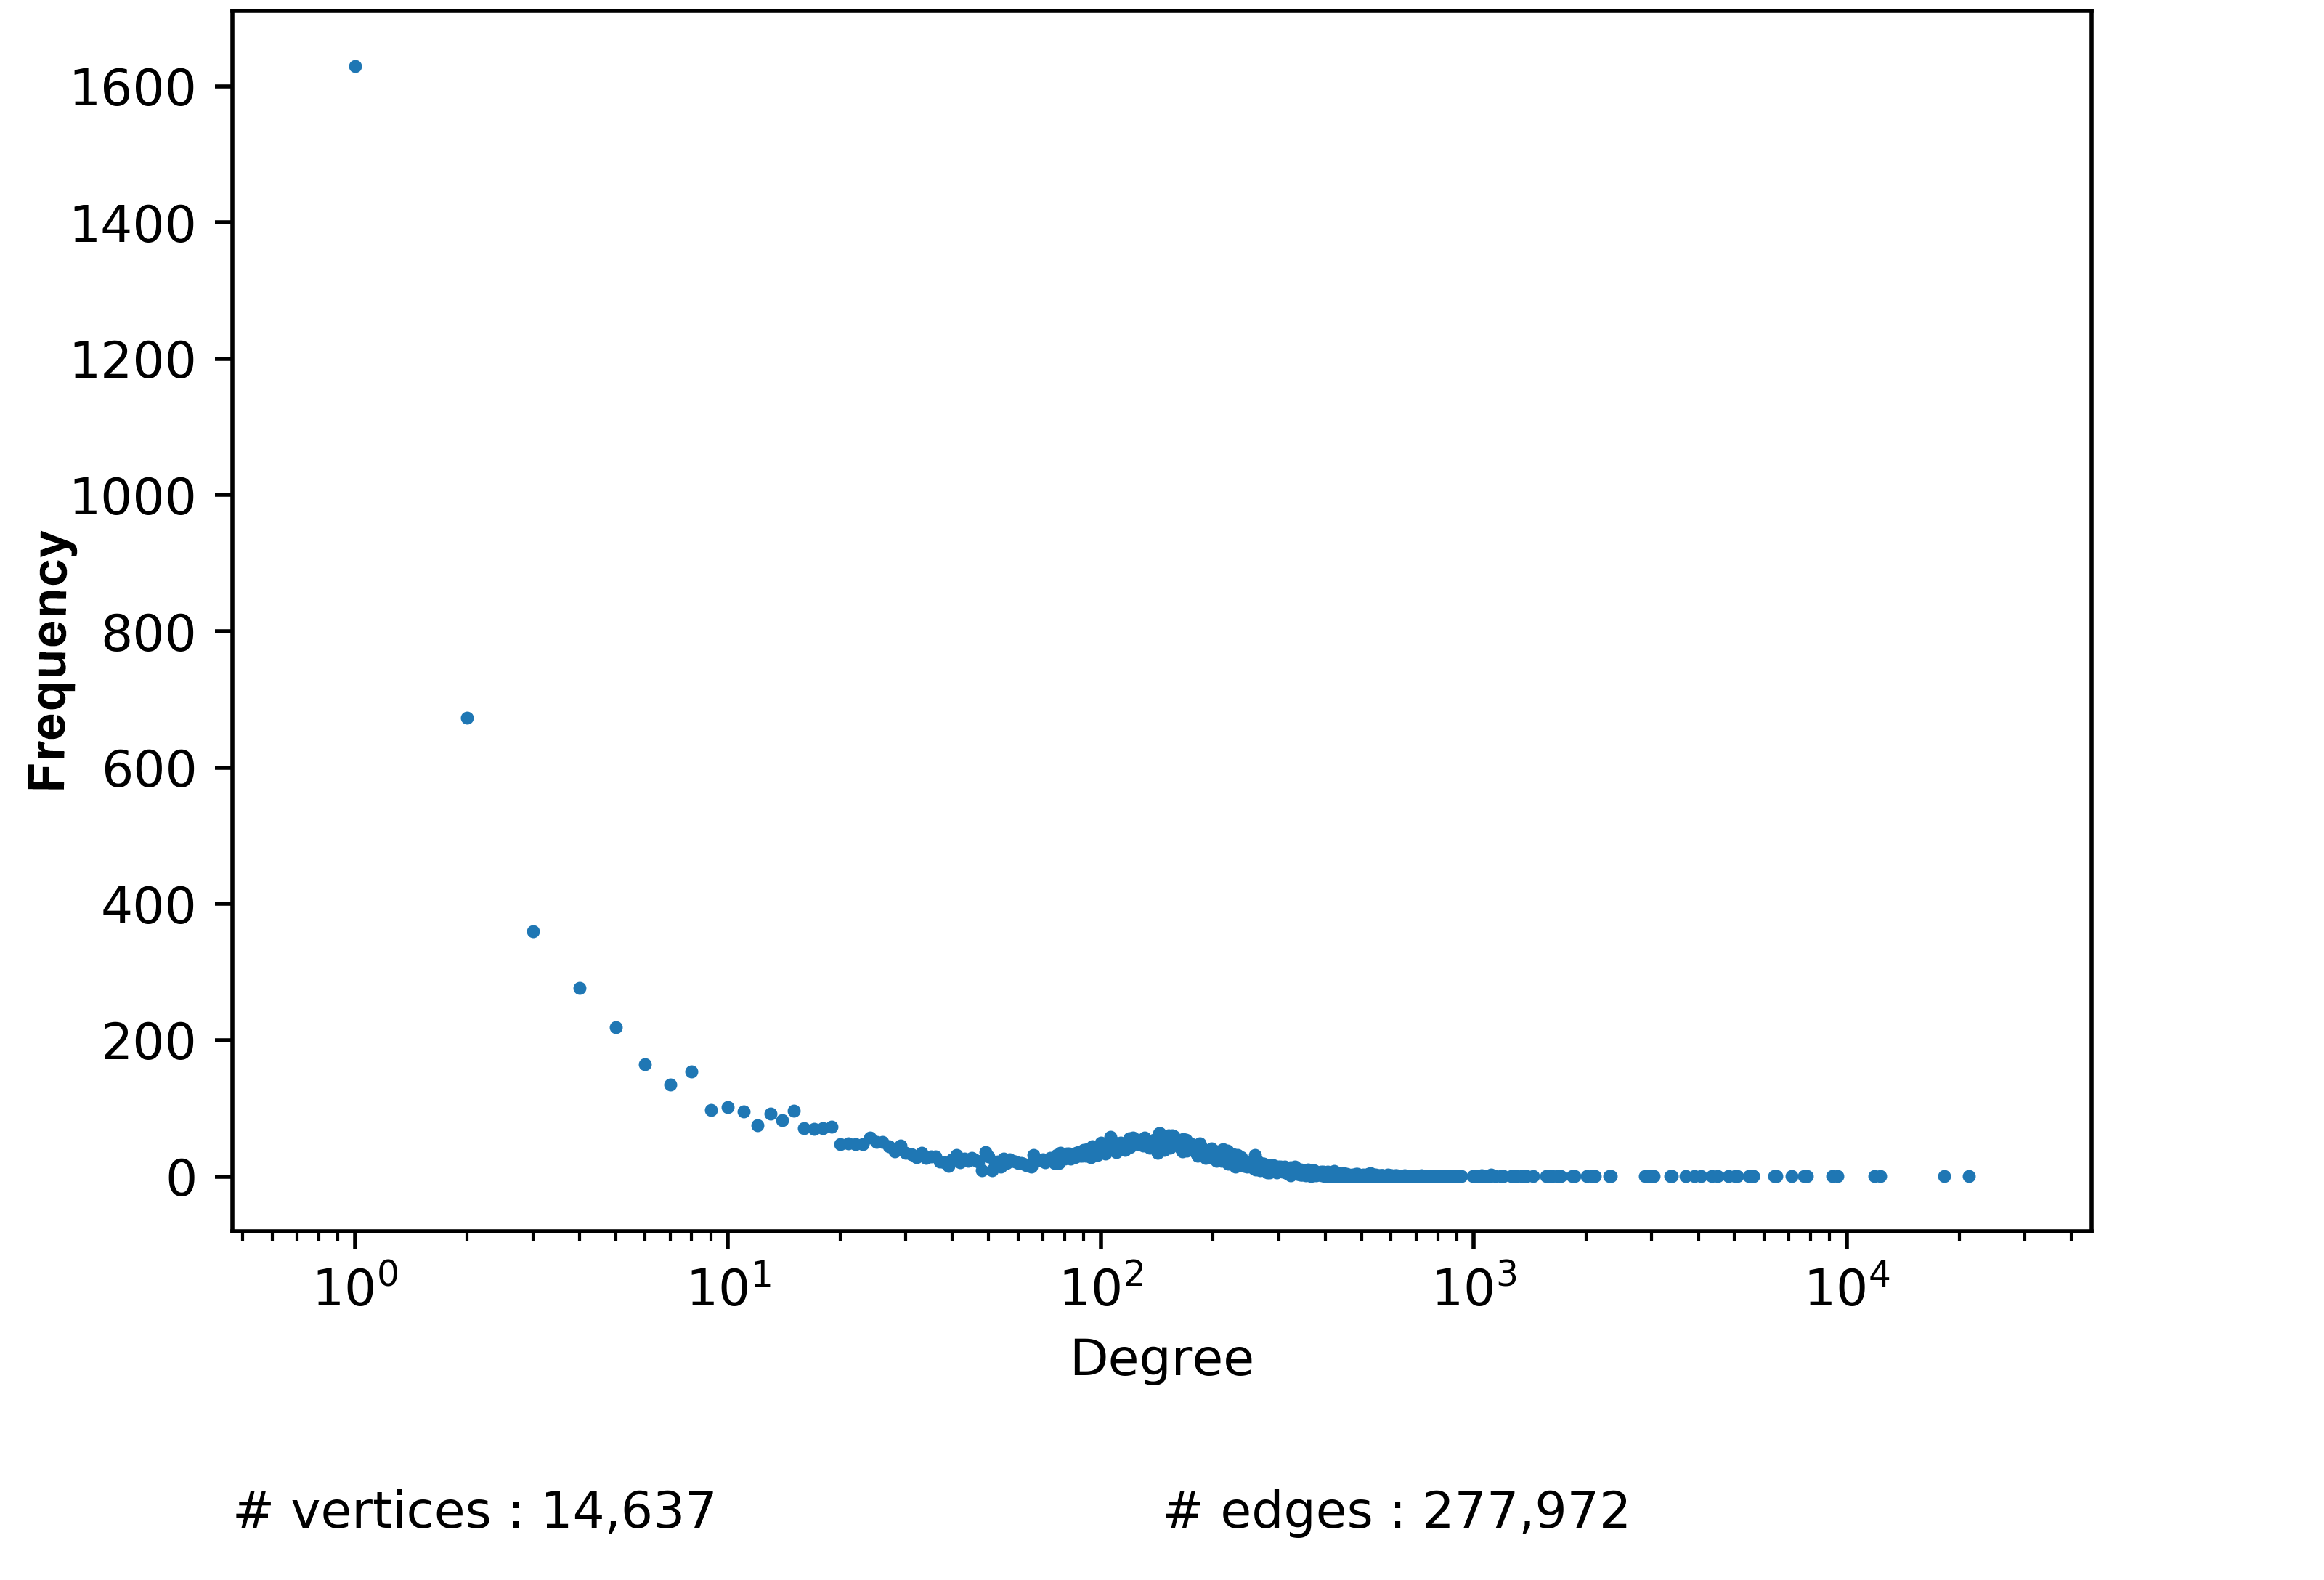
\includegraphics[width=0.85\textwidth]{results/dd/unicorn-wget-dd-alpha_1024}
    \vspace{-0.5cm}
    \caption{Degree distribution of Alpha for unicorn-wget dataset}
    \label{fig:unicorn-wget-dd-alpha_1024}
\end{figure}

\subsection*{Observations and inferences}

\paragraph{}
The graphs depicted by the summarized sketches in \autoref{fig:unicorn-wget-dd-countmin_1024}, \autoref{fig:unicorn-wget-dd-gsketch_1024}, \autoref{fig:unicorn-wget-dd-tcm_1024}, \autoref{fig:unicorn-wget-dd-gmatrix_1024} and \autoref{fig:unicorn-wget-dd-alpha_1024} have the same shape of the degree distribution as that of the original graph depicted in \autoref{fig:unicorn-wget-dd-fullgraph}. Thus all the sketches have preserved the degree distribution property of the original graph to a certain extent.
\section{Edge-weight distribution}

\subsection*{Purpose}

\paragraph{}
To compare the edge weight distribution of the original graph stream and the graph depicted by the summarized sketch.

\subsection*{Results}

\begin{figure}[H]
    \centering 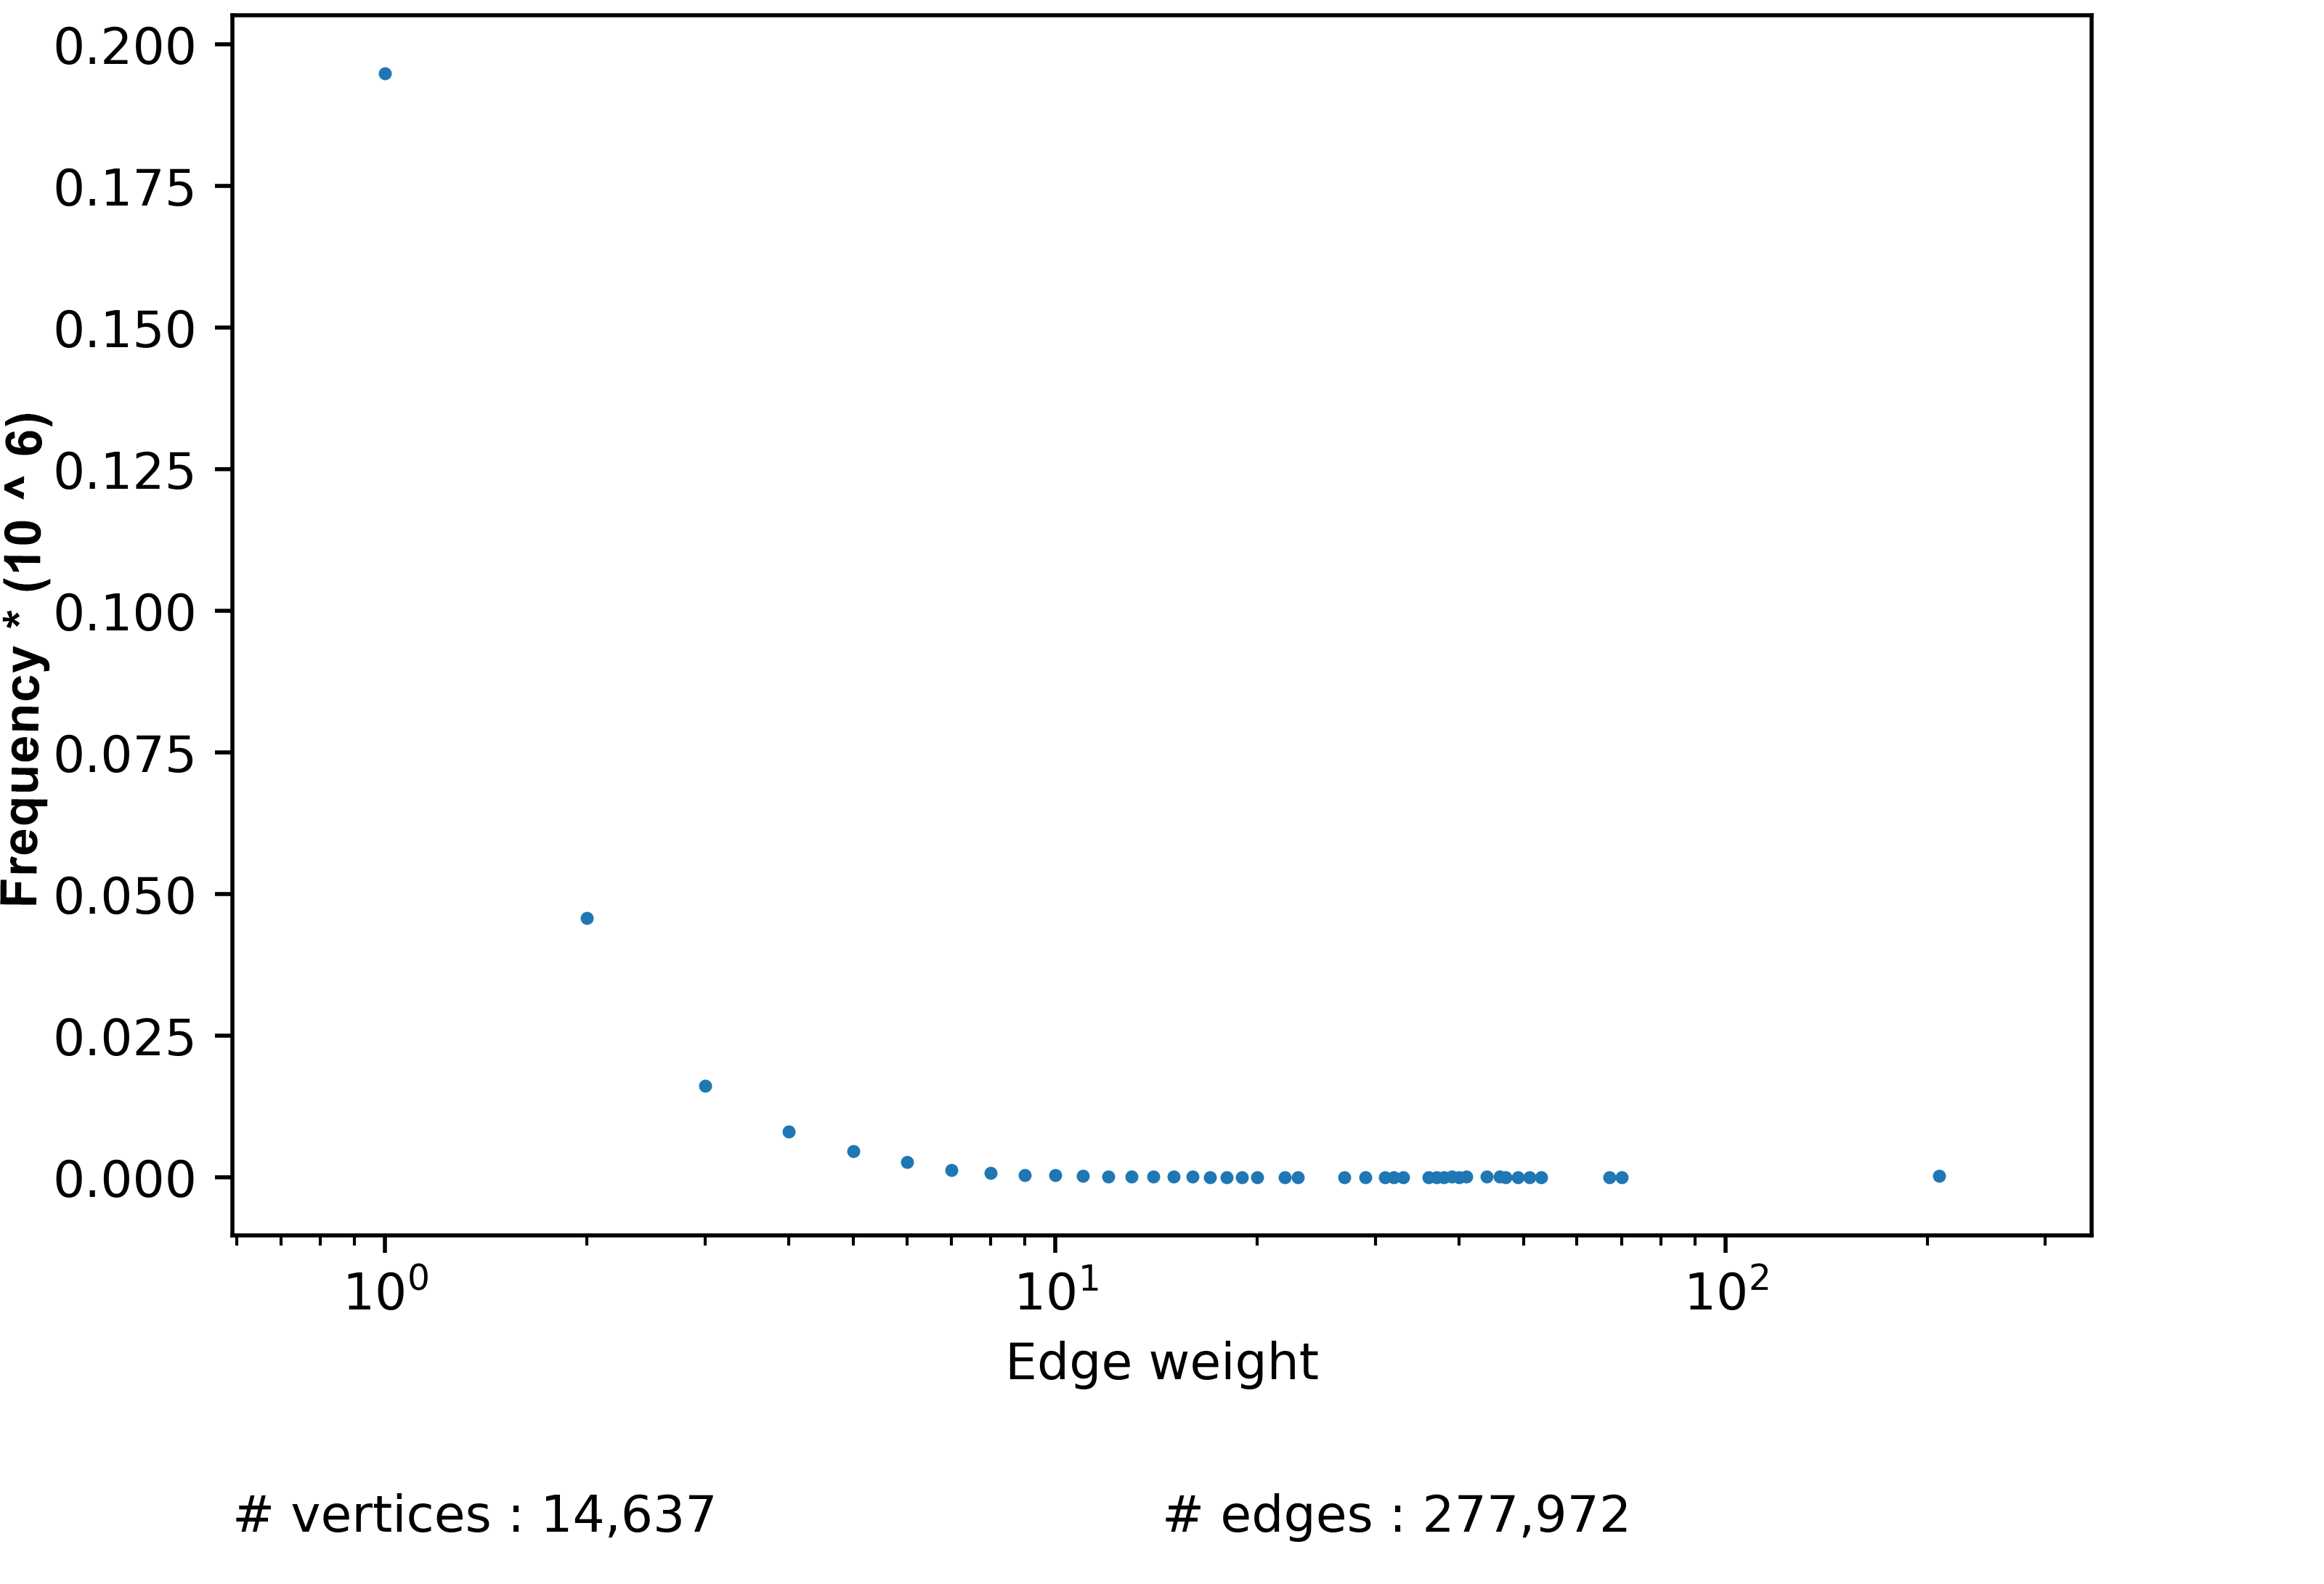
\includegraphics[width=0.85\textwidth]{results/ewd/unicorn-wget-ewd-fullgraph}
    \vspace{-0.5cm}
    \caption{Edge weight distribution of FullGraph for unicorn-wget dataset}
    \label{fig:unicorn-wget-ewd-fullgraph}
\end{figure}

\begin{figure}[H]
    \centering 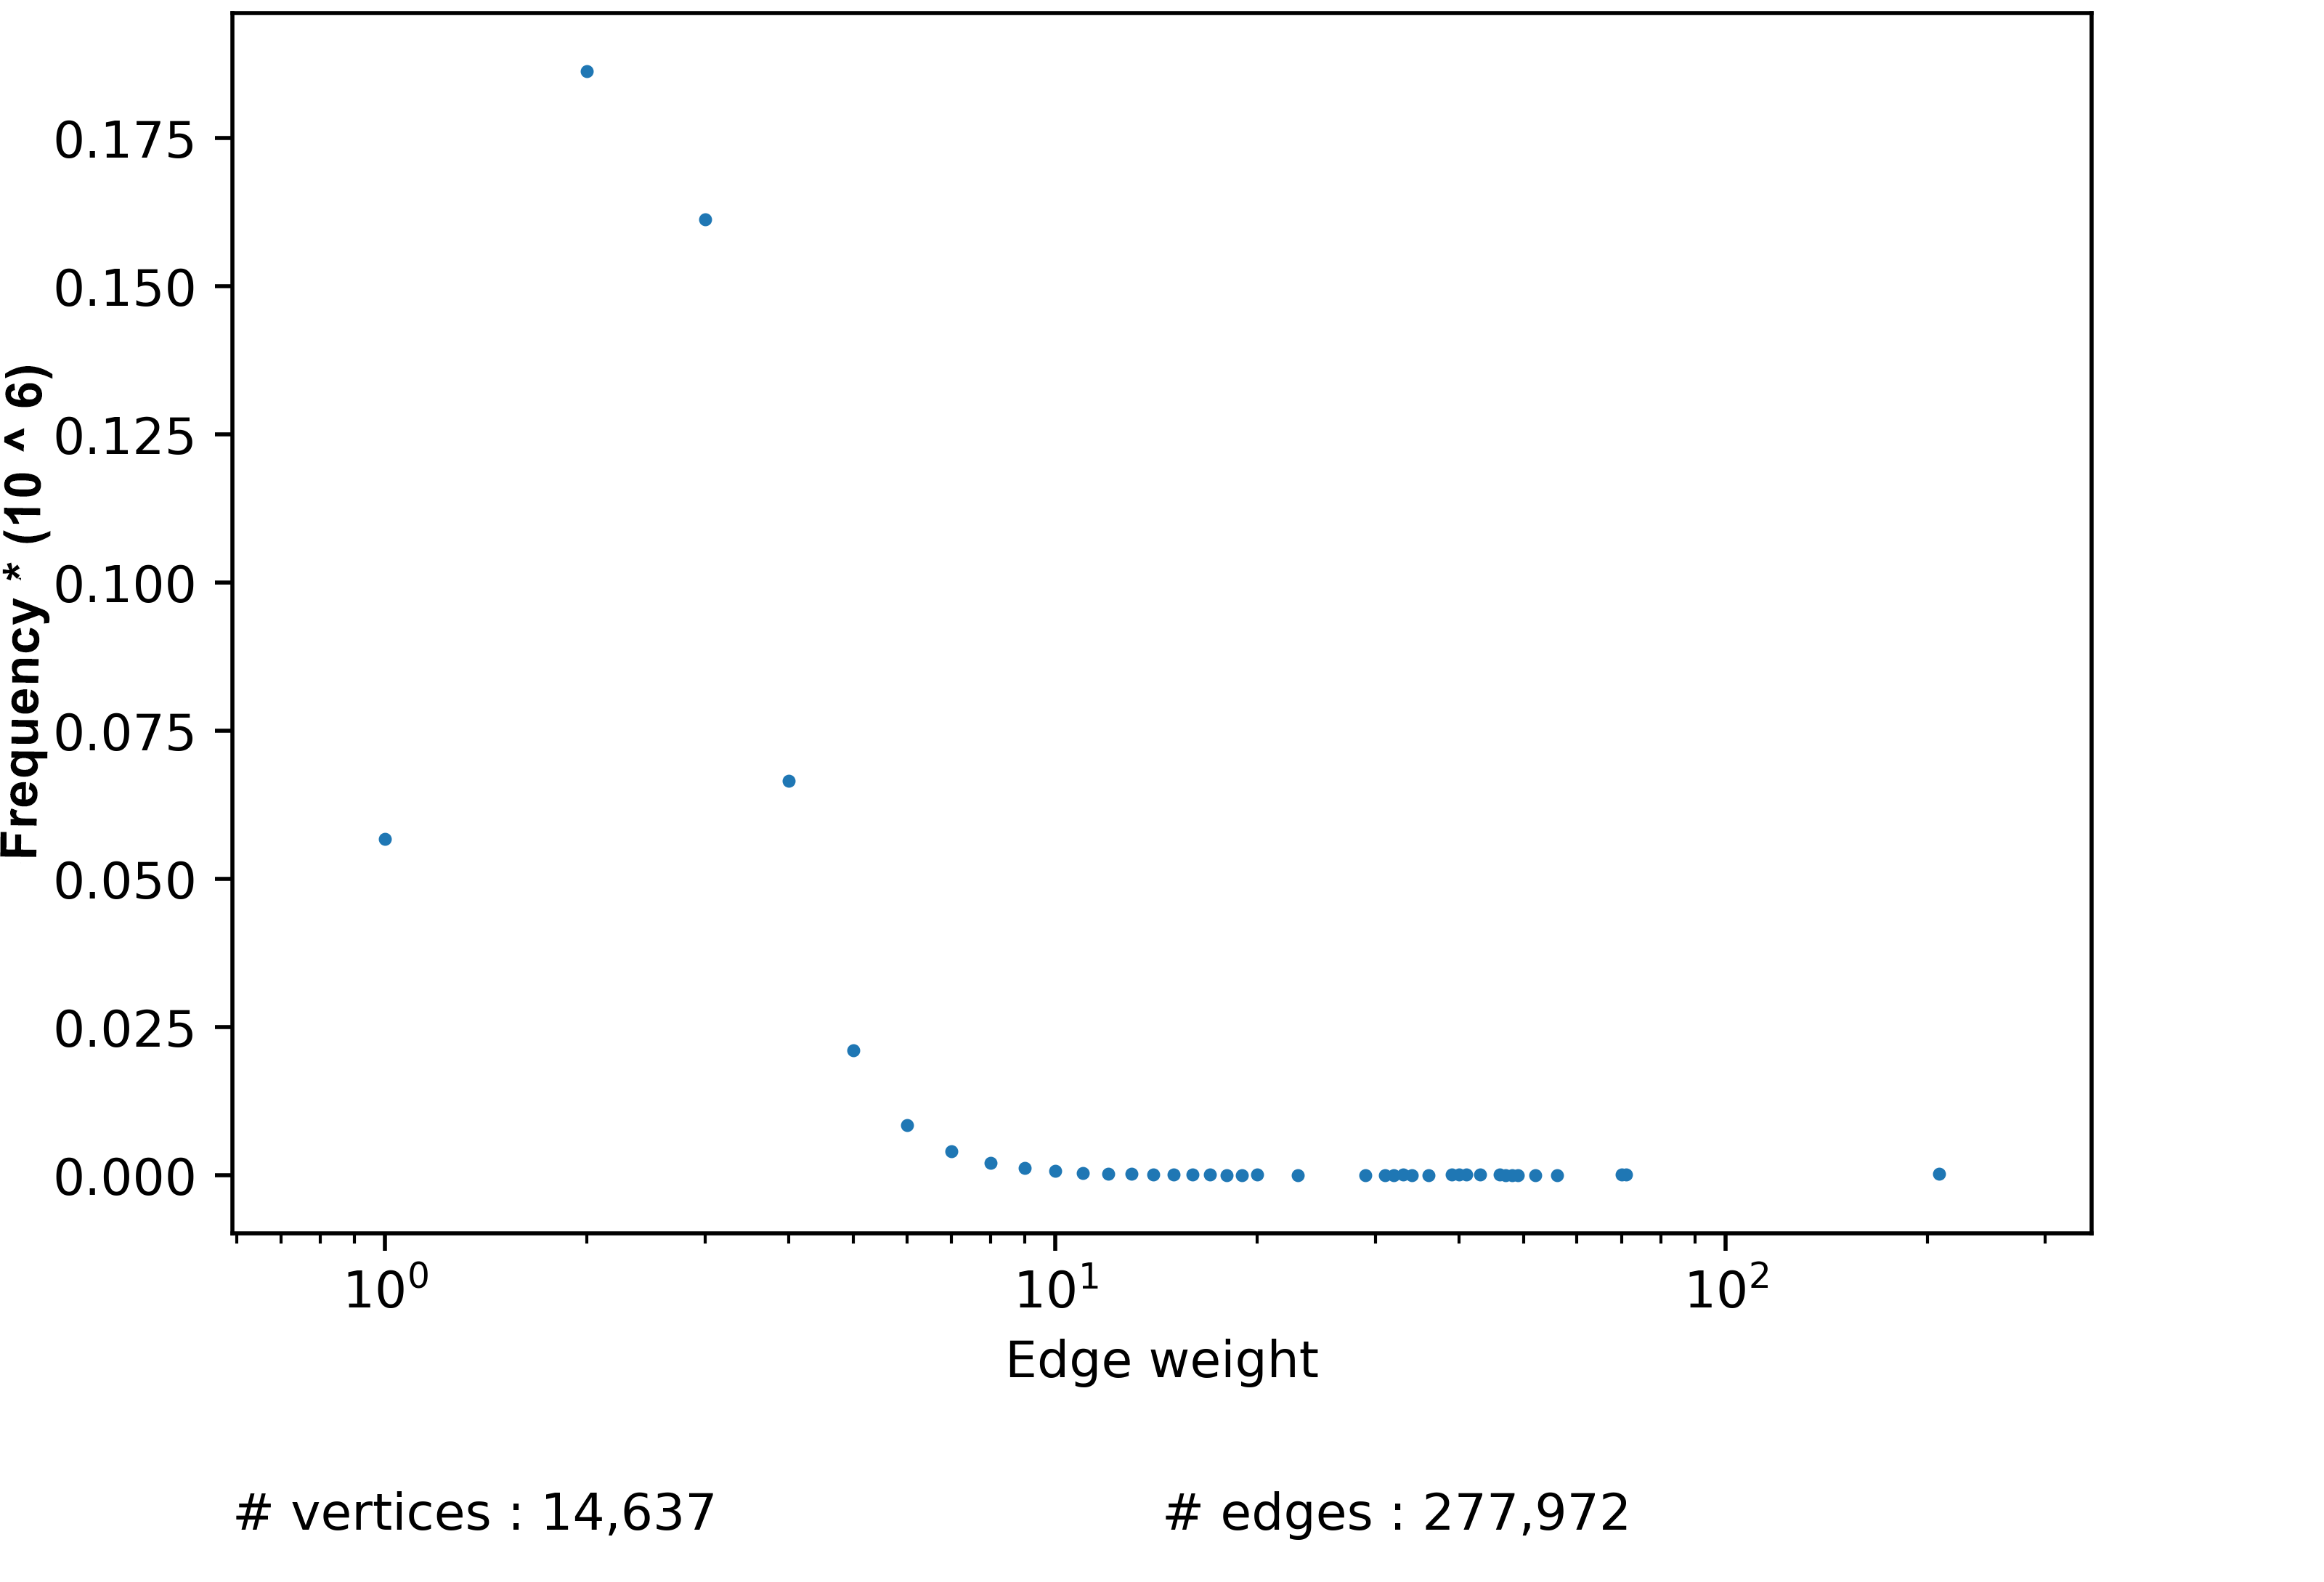
\includegraphics[width=0.85\textwidth]{results/ewd/unicorn-wget-ewd-countmin_1024}
    \vspace{-0.5cm}
    \caption{Edge weight distribution of CountMin for unicorn-wget dataset}
    \label{fig:unicorn-wget-ewd-countmin_1024}
\end{figure}

\begin{figure}[H]
    \centering 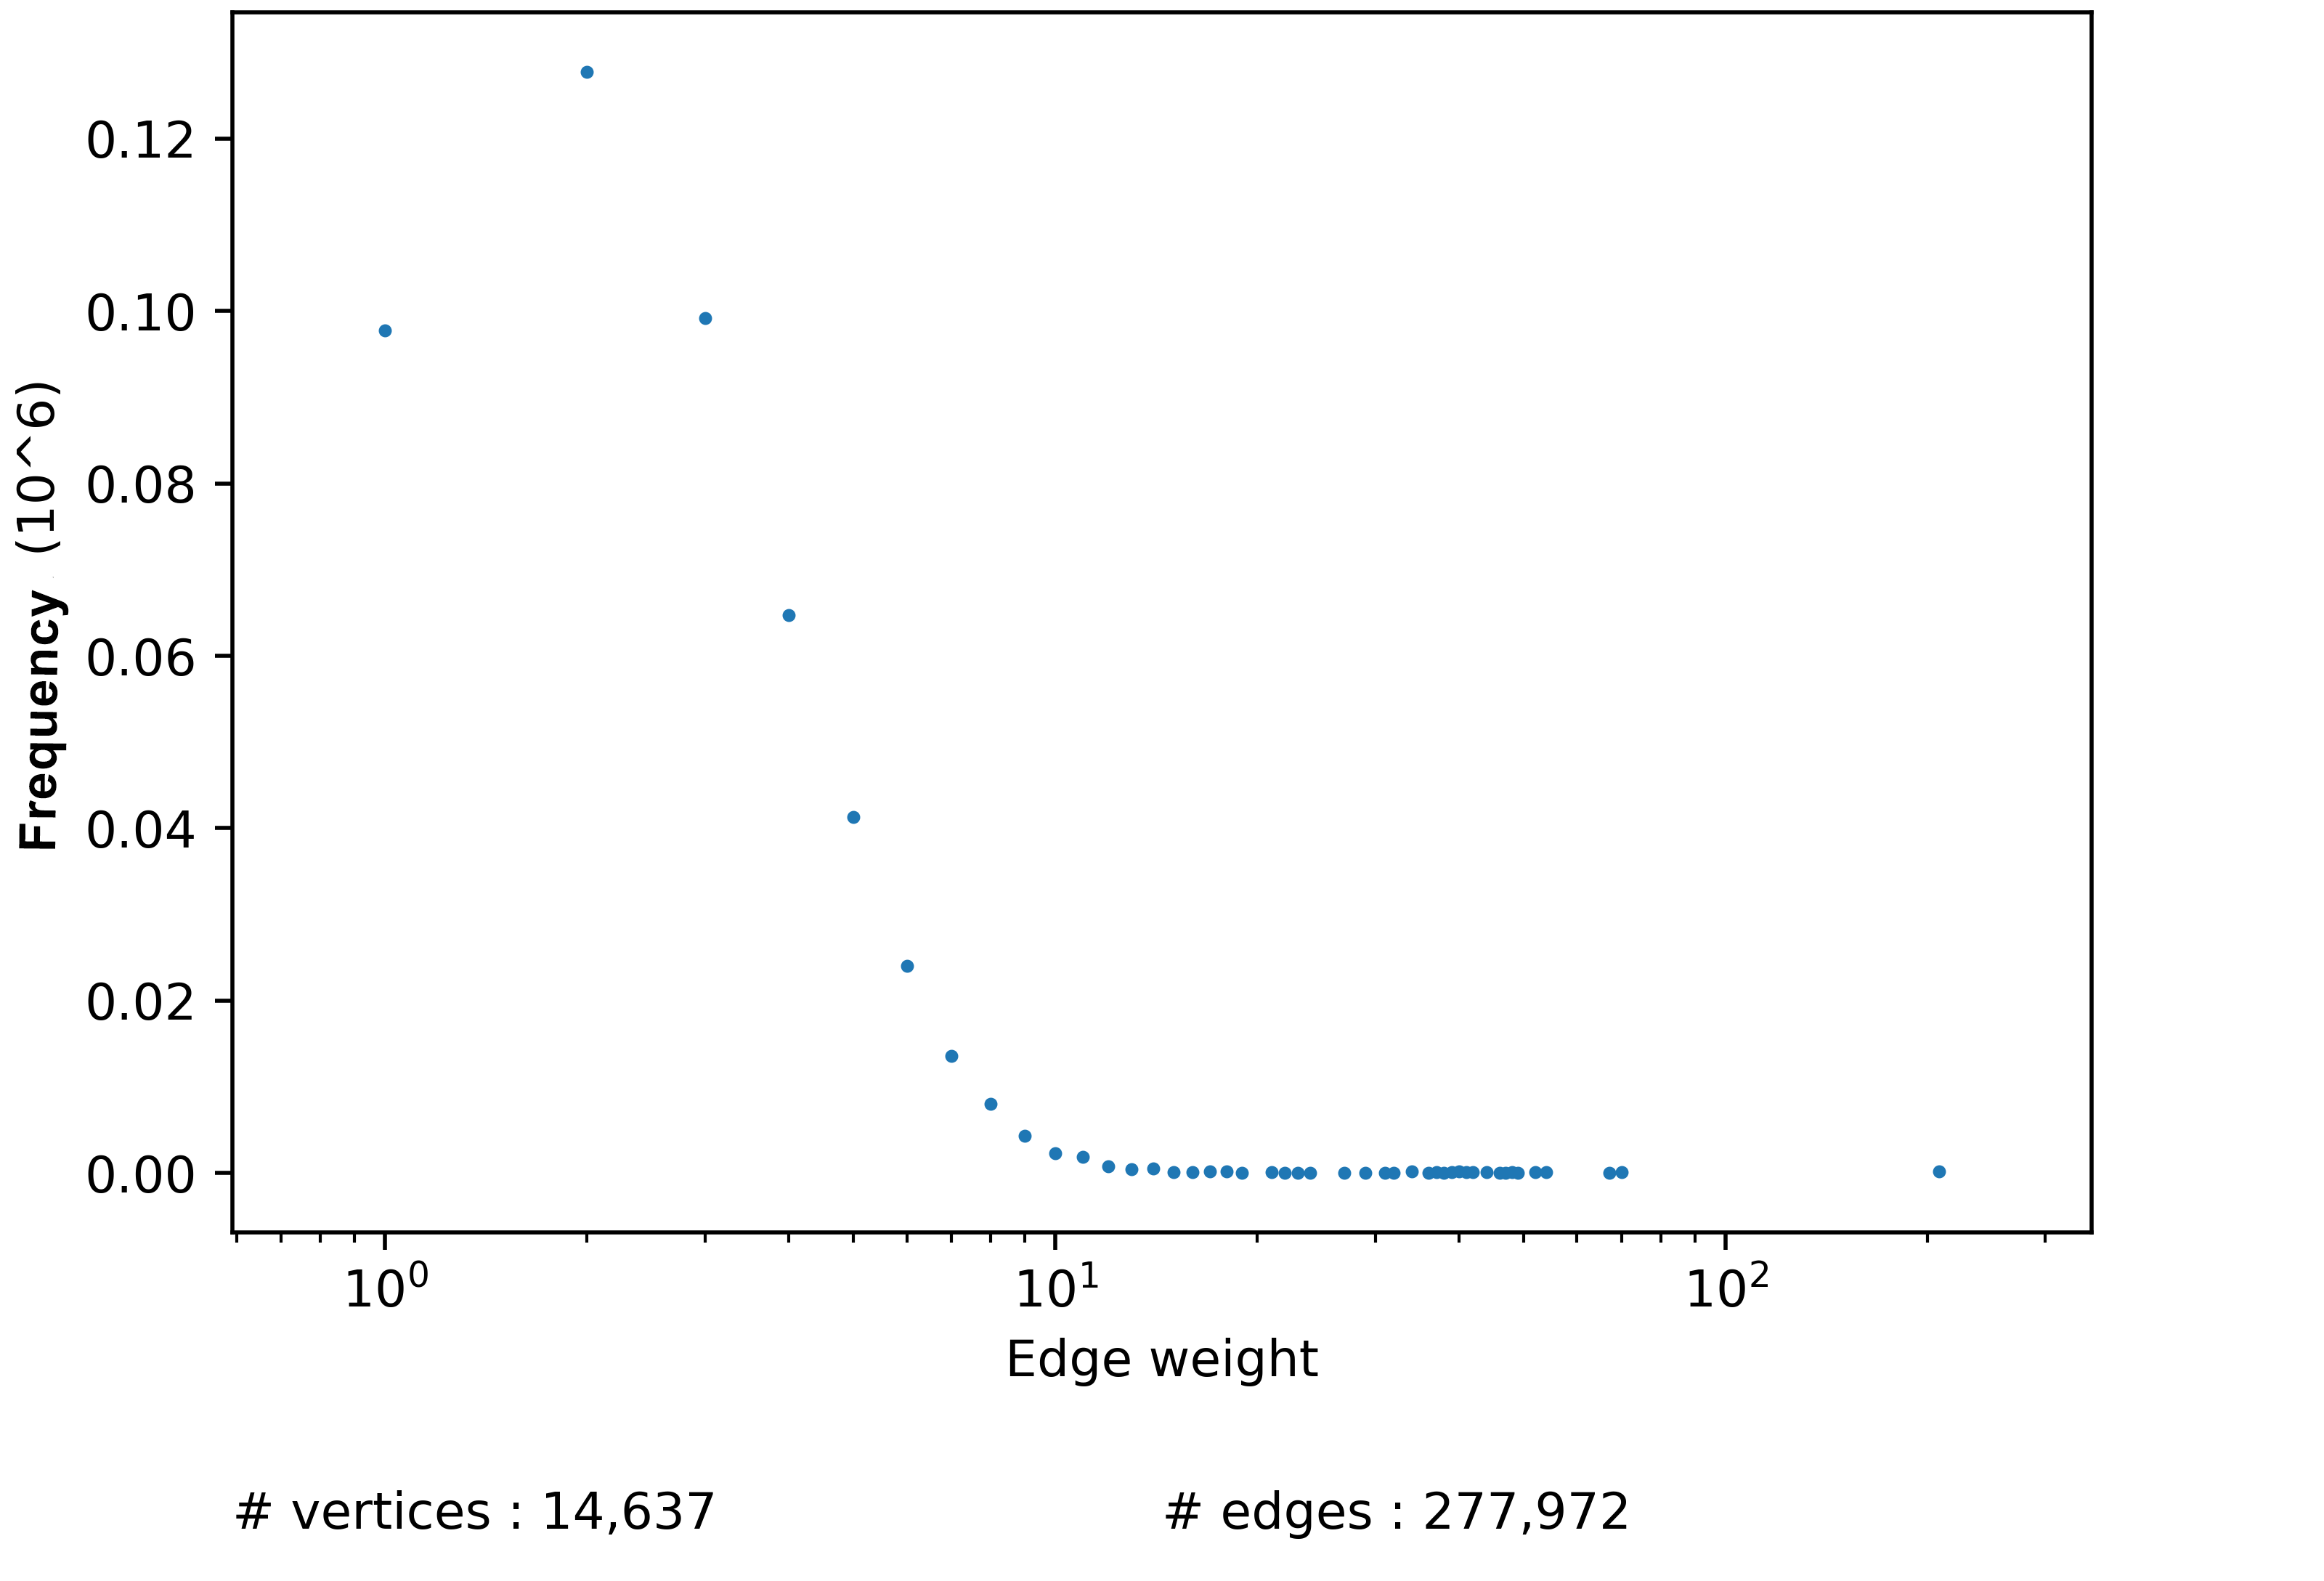
\includegraphics[width=0.85\textwidth]{results/ewd/unicorn-wget-ewd-gsketch_1024}
    \vspace{-0.5cm}
    \caption{Edge weight distribution of gSketch for unicorn-wget dataset}
    \label{fig:unicorn-wget-ewd-gsketch_1024}
\end{figure}

\begin{figure}[H]
    \centering 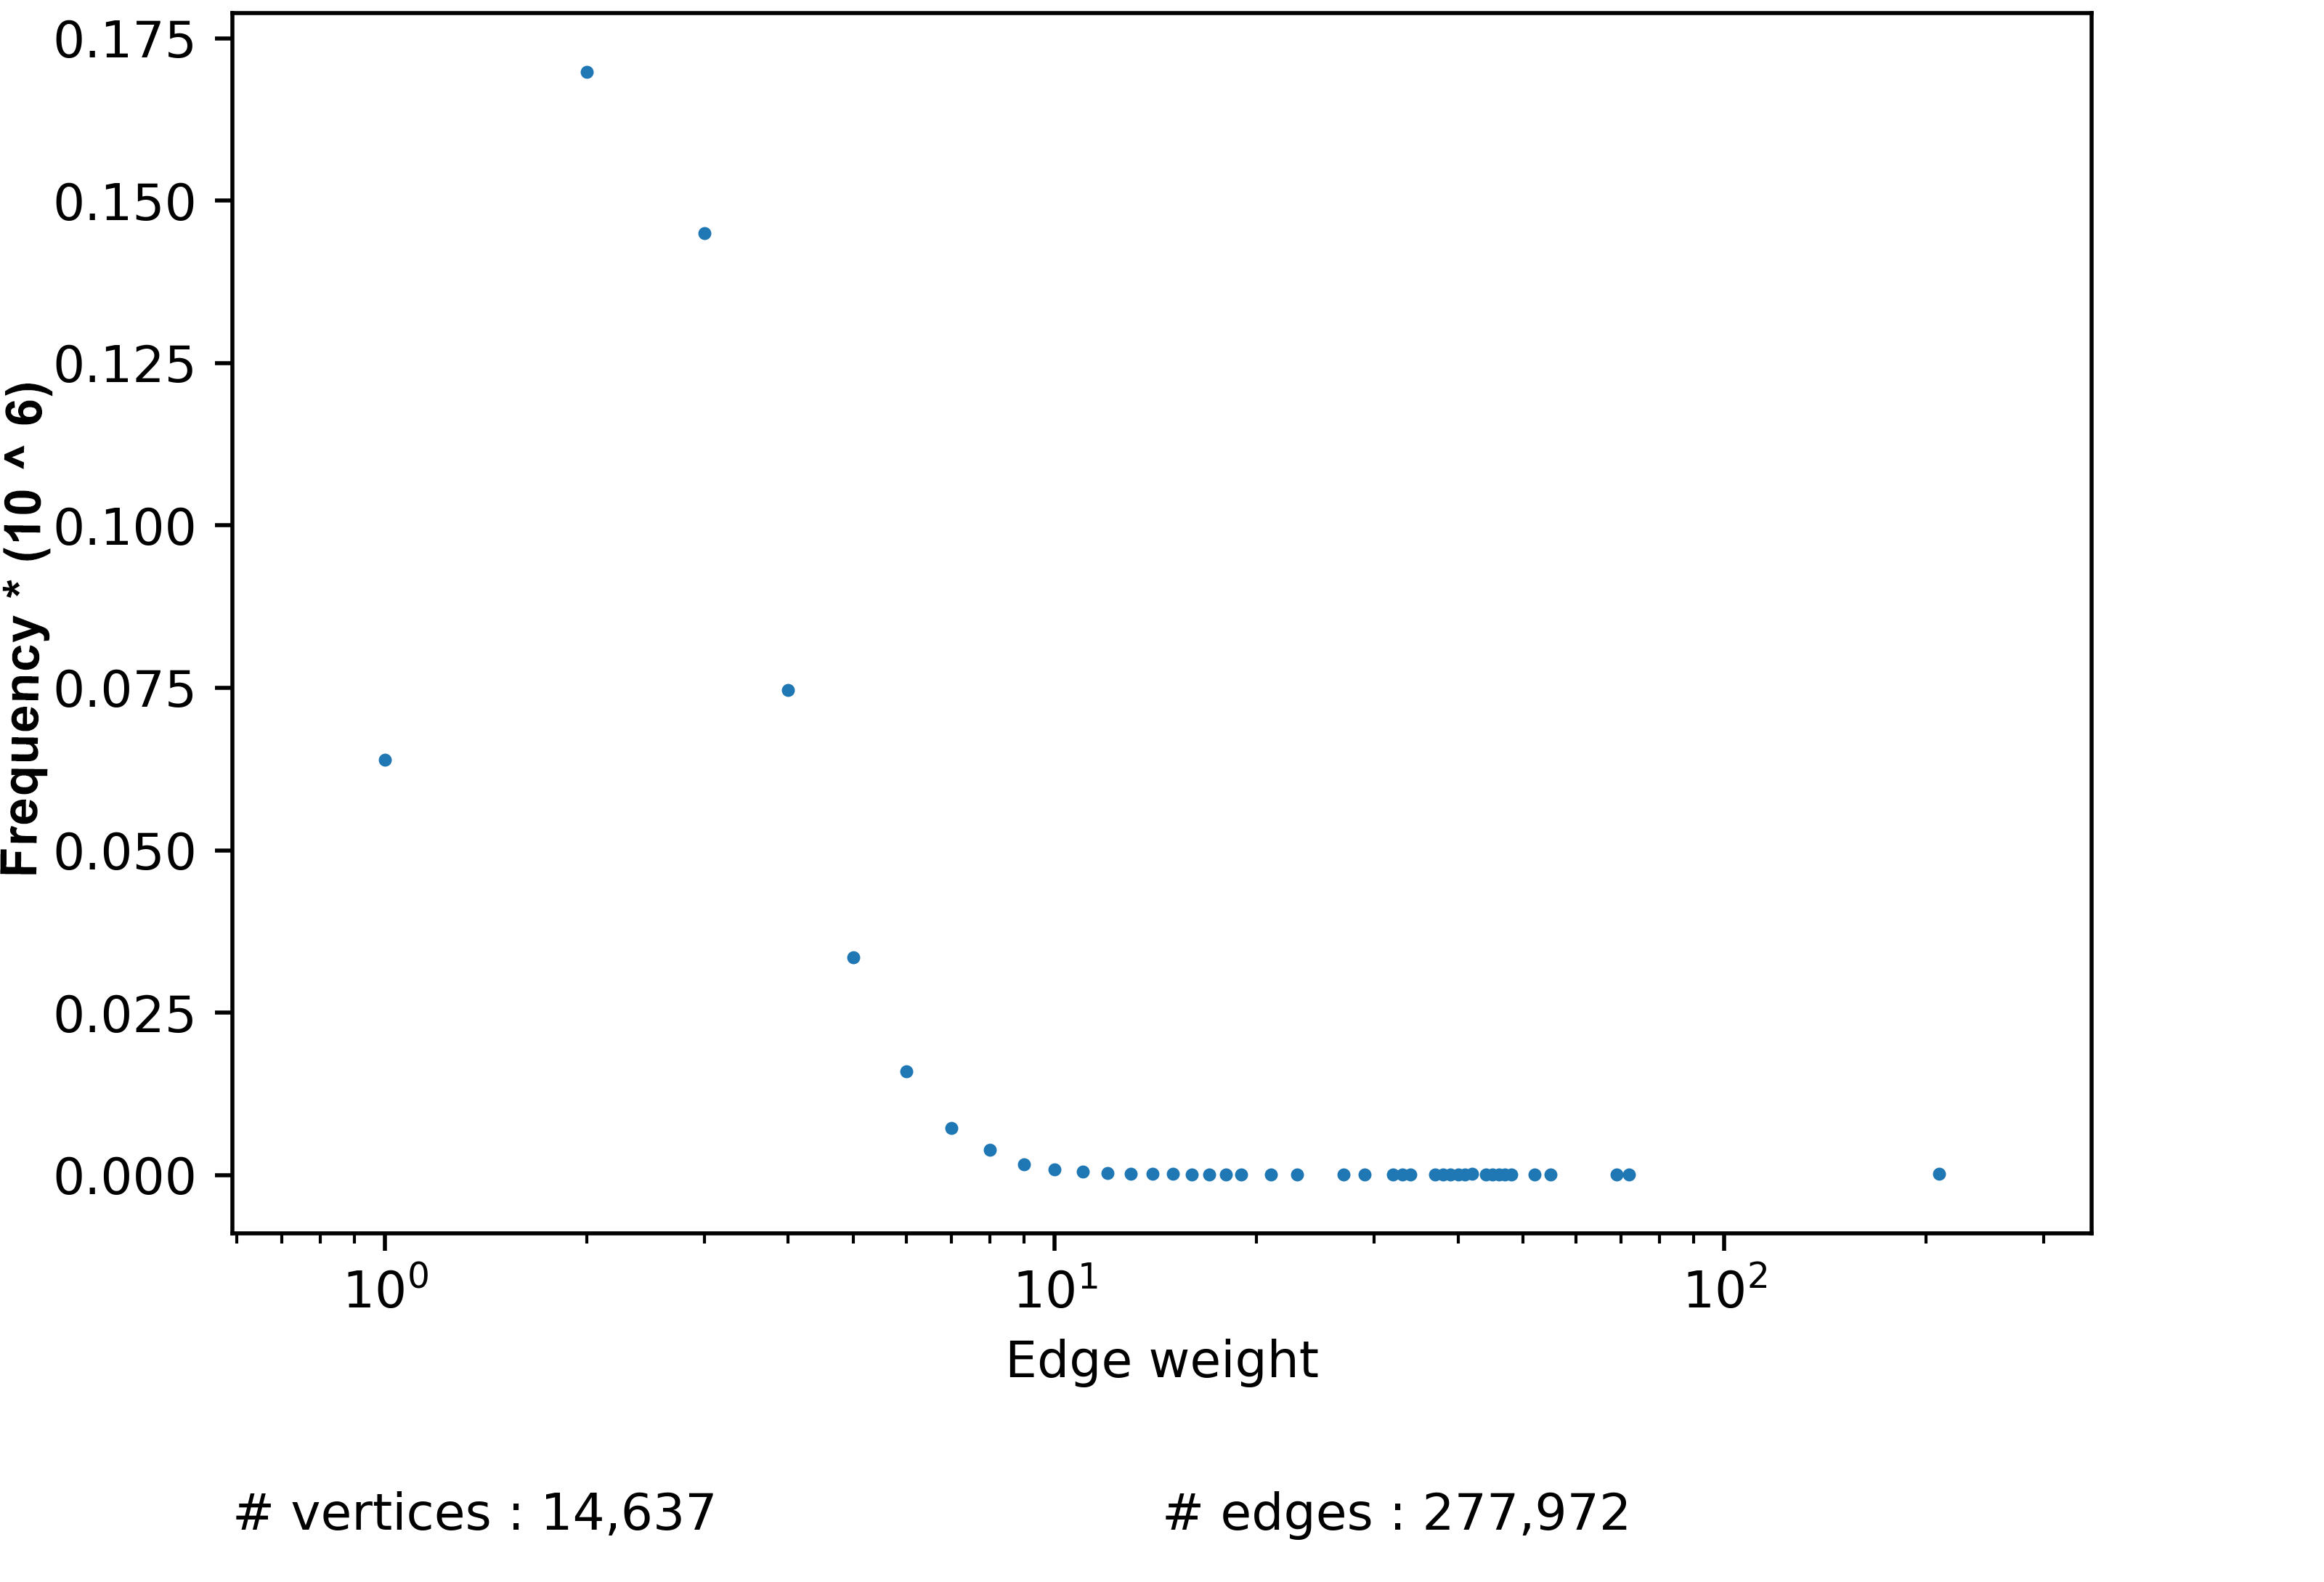
\includegraphics[width=0.85\textwidth]{results/ewd/unicorn-wget-ewd-tcm_1024}
    \vspace{-0.5cm}
    \caption{Edge weight distribution of TCM for unicorn-wget dataset}
    \label{fig:unicorn-wget-ewd-tcm_1024}
\end{figure}

\begin{figure}[H]
    \centering 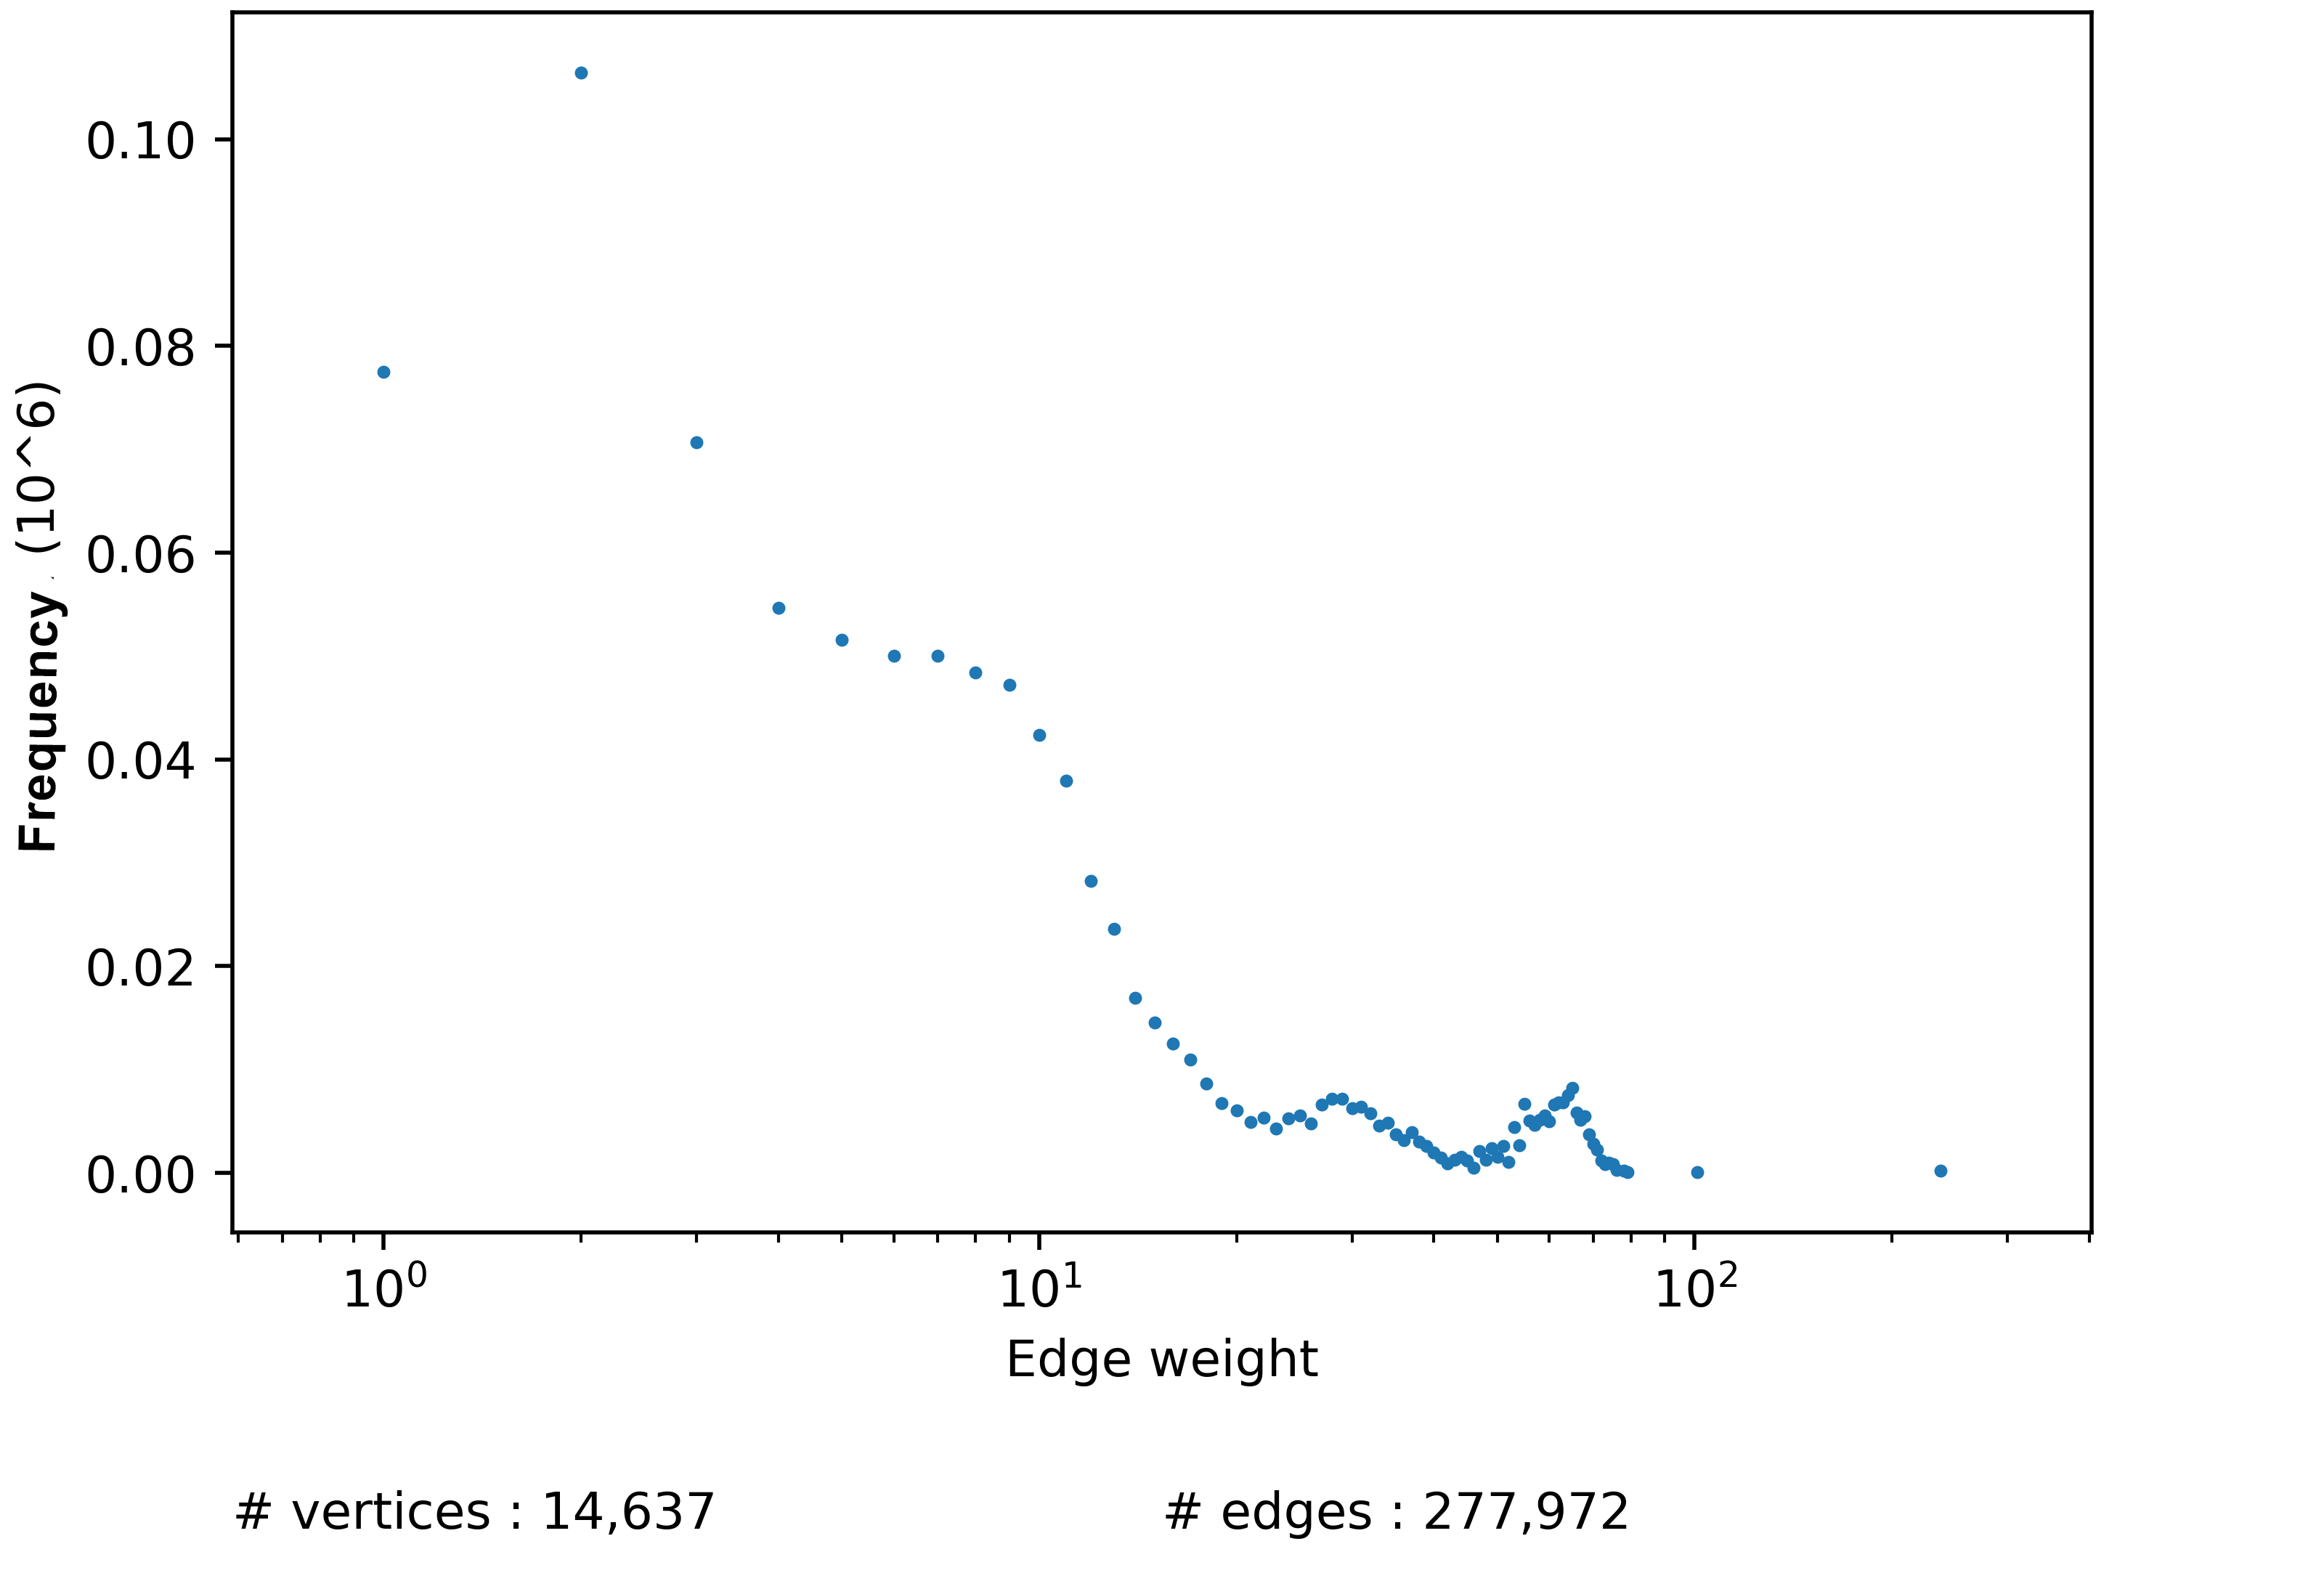
\includegraphics[width=0.85\textwidth]{results/ewd/unicorn-wget-ewd-gmatrix_1024}
    \vspace{-0.5cm}
    \caption{Edge weight distribution of GMatrix for unicorn-wget dataset}
    \label{fig:unicorn-wget-ewd-gmatrix_1024}
\end{figure}

\begin{figure}[H]
    \centering \includegraphics[width=0.85\textwidth]{results/ewd/unicorn-wget-ewd-alpha_1024}
    \vspace{-0.5cm}
    \caption{Edge weight distribution of Alpha for unicorn-wget dataset}
    \label{fig:unicorn-wget-ewd-alpha_1024}
\end{figure}

\subsection*{Observations and inferences}

\paragraph{}
CountMin in \autoref{fig:unicorn-wget-ewd-countmin_1024}, gSketch in \autoref{fig:unicorn-wget-ewd-gsketch_1024} and TCM in \autoref{fig:unicorn-wget-ewd-tcm_1024} have preserved the shape of the original edge weight distribution depicted in \autoref{fig:unicorn-wget-ewd-fullgraph}. However Alpha in \autoref{fig:unicorn-wget-ewd-alpha_1024} has a slightly distorted distribution shape while the GMatrix in \autoref{fig:unicorn-wget-ewd-gmatrix_1024} has some significant changes with respect to the original stream.

\subsection*{Conclusion}

\paragraph{}
The proposed sketch Alpha is not a good candidate for preserving the edge weight distribution of a graph stream.
\section{Edge insertion time}

\paragraph{}
To see the effect of,

\begin{itemize}
    \item Memory allocation
    \item Number of edges already present in the sketch
\end{itemize}

on the speed of the edge operations.

\subsection*{Memory allocation}

\subsubsection{Purpose}

\paragraph{}
To analyze the speed of the edge operations (insertion) with respect to memory allocated for the sketch.

\subsubsection{Results}

\begin{figure}[H]
    \centering \includegraphics[width=0.85\textwidth]{results/insertion/unicorn-wget-insertiontime1}
    \vspace{-0.5cm}
    \caption{Insertion time per edge vs Memory for unicorn-wget dataset}
    \label{fig:unicorn-wget-insertiontime1}
\end{figure}

\begin{figure}[H]
    \centering \includegraphics[width=0.85\textwidth]{results/insertion/email-EuAll-insertiontime1}
    \vspace{-0.5cm}
    \caption{Insertion time per edge vs Memory for email-EuAll dataset}
    \label{fig:email-EuAll-insertiontime1}
\end{figure}

\begin{figure}[H]
    \centering \includegraphics[width=0.85\textwidth]{results/insertion/cit-HepPh-insertiontime1}
    \vspace{-0.5cm}
    \caption{Insertion time per edge vs Memory for cit-HepPh dataset}
    \label{fig:cit-HepPh-insertiontime1}
\end{figure}

\begin{figure}[H]
    \centering \includegraphics[width=0.85\textwidth]{results/insertion/gen-scale-free-insertiontime1}
    \vspace{-0.5cm}
    \caption{Insertion time per edge vs Memory for gen-scale-free dataset}
    \label{fig:gen-scale-free-insertiontime1}
\end{figure}

\begin{figure}[H]
    \centering \includegraphics[width=0.85\textwidth]{results/insertion/gen-small-world-insertiontime1}
    \vspace{-0.5cm}
    \caption{Insertion time per edge vs Memory for gen-small-world dataset}
    \label{fig:gen-small-world-insertiontime1}
\end{figure}

\subsubsection{Observations and inferences}

\paragraph{}
The proposed sketch Alpha shows faster speeds of insertion operations on the datasets, unicorn-wget in \autoref{fig:unicorn-wget-insertiontime1}, cit-HepPh in \autoref{fig:cit-HepPh-insertiontime1} and gen-small-world in \autoref{fig:gen-small-world-insertiontime1}. However this is not the case for email-EuAll in \autoref{fig:email-EuAll-insertiontime1} and gen-scale-free in \autoref{fig:gen-scale-free-insertiontime1}.

\paragraph{}
TCM has yielded the slowest insertion speeds despite the type of the dataset while gSketch has achieved the highest speed for all the datasets.

\subsubsection{Conclusion}

\paragraph{}
gSketch is the suitable type of sketching technique in a scenario where the edge operation speeds are critical.

\subsection*{Number of edges already present in the sketch}

\subsubsection{Purpose}

\paragraph{}
To analyze the speed of the edge operations (insertion) with respect to number of edges that is already present in the sketch.

\subsubsection{Results}

\begin{figure}[H]
    \centering \includegraphics[width=0.85\textwidth]{results/insertion/unicorn-wget-insertiontime2_512}
    \vspace{-0.5cm}
    \caption{Insertion time per edge vs Number of edges in the sketch for unicorn-wget dataset}
    \label{fig:unicorn-wget-insertiontime2_512}
\end{figure}

\begin{figure}[H]
    \centering \includegraphics[width=0.85\textwidth]{results/insertion/email-EuAll-insertiontime2_512}
    \vspace{-0.5cm}
    \caption{Insertion time per edge vs Number of edges in the sketch for email-EuAll dataset}
    \label{fig:email-EuAll-insertiontime2_512}
\end{figure}

\begin{figure}[H]
    \centering \includegraphics[width=0.85\textwidth]{results/insertion/cit-HepPh-insertiontime2_512}
    \vspace{-0.5cm}
    \caption{Insertion time per edge vs Number of edges in the sketch for cit-HepPh dataset}
    \label{fig:cit-HepPh-insertiontime2_512}
\end{figure}

\begin{figure}[H]
    \centering \includegraphics[width=0.85\textwidth]{results/insertion/gen-scale-free-insertiontime2_512}
    \vspace{-0.5cm}
    \caption{Insertion time per edge vs Number of edges in the sketch for gen-scale-free dataset}
    \label{fig:gen-scale-free-insertiontime2_512}
\end{figure}

\begin{figure}[H]
    \centering \includegraphics[width=0.85\textwidth]{results/insertion/gen-small-world-insertiontime2_512}
    \vspace{-0.5cm}
    \caption{Insertion time per edge vs Number of edges in the sketch for gen-small-world dataset}
    \label{fig:gen-small-world-insertiontime2_512}
\end{figure}

\subsubsection{Observations and inferences}

\paragraph{}
The speed of the edge operations (insertions) doesn't show a steady increase nor a decrease with respect to the amount of data in the sketch for the datasets depicted in \autoref{fig:unicorn-wget-insertiontime2_512}, \autoref{fig:cit-HepPh-insertiontime2_512}, \autoref{fig:gen-scale-free-insertiontime2_512} or \autoref{fig:gen-small-world-insertiontime2_512}.

\paragraph{}
\autoref{fig:email-EuAll-insertiontime2_512} of the dataset email-EuAll shows a steady increase of the insertion time per edge for the Alpha and gSketch sketches. We can infer that this is a result of the specific partitioning structure created for that particular dataset with the given parameters.

\paragraph{}
There is no direct correlation between the time per insertion operation and the number of edges present in the sketch. Thus we can conclude that there is no causation between the aforementioned properties as well.
\section{Summary}

\paragraph{}
This chapter gives an introduction to the most relevant related work for this research. Throughout this chapter, the representations of graphs in computers, real world graphs, graph summarization had been explained giving much focus to streaming graph summarization. The dissertation will address the research design in the next chapter.

% \section{Clustering}

\todo

\subsection*{Purpose}

\todo

\subsection*{Results}

\todo

\subsection*{Observations and inferences}

\todo

\subsection*{Conclusion}

\todo
% \section{PageRank}

\subsubsection{Purpose}

\todo

\subsubsection{Results}

\todo

\subsubsection{Observations and inferences}

\todo

\subsubsection{Conclusion}

\todo
\chapter{Conclusions}

\section{Introduction}

\paragraph{}
This chapter will discuss the conclusion of the research in \autoref{section:conclusion_rq} and \autoref{section:conclusion_rp}. Limitations of the carried out work will be discussed in \autoref{section:conclusion_limitations}. The chapter will conclude after discussing the future work of the research in brief in \autoref{section:conclusion_future}.

\section{Conclusion about research questions}
\label{section:conclusion_rq}

\paragraph{}
The first research question in \autoref{section:research_questions} is, \textit{‘What are the tradeoffs of existing graph summarization techniques?’}. The tradeoffs of existing graph summarization techniques have been discussed thoroughly in \autoref{section:results_n_evaluation} with respect to different graph properties.

\paragraph{}
The second research question in \autoref{section:research_questions} is, \textit{‘How to improve upon existing streaming graph summarization sketches in order to increase the accuracy of the queries answered through these sketches while keeping the memory constant?’}. The Alpha sketch has been proposed through this research as an extension for the GMatrix sketch using the sketch partitioning technique. It is able to answer queries with a significantly lower average relative error with the same amount of memory in comparison to the existing state-of-the-art sketching technique, TCM, as indicated in \autoref{section:results_are}. Thus Alpha answers the second research question on a way to improve the accuracy of the queries over the existing sketching techniques.

\section{Conclusion about research problem}
\label{section:conclusion_rp}

\paragraph{}
There are many streaming graph summarization algorithms. However, there doesn’t exist a proper survey on streaming graph summarization, benchmarking all these algorithms against each other. We have achieved this during our research and produced a test suit that could be used to run the benchmarking tasks in the future. Furthermore, we have produced Alpha, an improved sketch over the existing sketching techniques which utilizes partitioning to reduce the average relative error of the queries.

\section{Limitations}
\label{section:conclusion_limitations}

\paragraph{}
A major limitation of the work that was carried out is the fact that the test suite was implemented in Python. This helped in reducing the implementation time of the test suite. However, as Python is an interpreted language, it is much slower than a low-level language than C or C++. Therefore the testing procedure took considerable time in running the sketching algorithms against the selected datasets. This was a clear hindrance on testing much larger datasets.

\section{Implications for further research}
\label{section:conclusion_future}

\paragraph{}
This is an embarrassingly parallel query framework model, therefore the model should be evaluated on top of a parallel framework. Furthermore, there are many aspects that could be considered before the Alpha sketch is to be used in a practical scenario such as sliding windows and data partitioning across multiple machines.

% References
\renewcommand\bibname{References}
\bibliographystyle{unsrt}
\bibliography{references}

\appendix

% Variables
\def\titlename{Realtime Property Evaluation of Large Streaming Graphs}
\def\authorname{O.I. Mudannayake}
\def\authorindexno{15000893}
\def\supervisorname{Dr. D.N. Ranasinghe}
\def\titledate{February 2020}
\def\signaturedate{18/02/2020}
\def\headertopright{Final Year Project in CS}
\def\headertopleft{Thesis}
\def\companyname{University of Colombo School of Computing}

\def\todo{{\color{purple}\# To be completed!}}

\chapter{Code Listings}
\label{appendix:codes}

\section{Preprocessor}
\label{appendix:preprocessor}
\pythonexternal{code_listings/preprocessor.py}

\section{timeit function}
\label{appendix:timeit}
\pythonexternal{code_listings/utils.py}

\section{CountMin}
\label{appendix:countmin}
\pythonexternal{code_listings/countmin.py}

\section{gSketch}
\label{appendix:gsketch}
\pythonexternal{code_listings/gsketch.py}

\section{TCM}
\label{appendix:tcm}
\pythonexternal{code_listings/tcm.py}

\section{GMatrix}
\label{appendix:gmatrix}
\pythonexternal{code_listings/gmatrix.py}

\section{Alpha}
\label{appendix:alpha}
\pythonexternal{code_listings/alpha.py}

\end{document}